\documentclass[a4paper]{amsart}
\usepackage[margin=3cm, marginpar=3cm]{geometry}

\title[The Heisenberg algebra of a vector space and Hochschild
homology]{The Heisenberg algebra of a vector space \\ and Hochschild homology}

\author{\'Ad\'am Gyenge}
\address{Budapest University of Technology and Economics, Department of Algebra and Geometry, M\H{u}egyetem rakpart 3-9., 1111, Budapest, Hungary}
\email{Gyenge.Adam@ttk.bme.hu}

\author{Timothy Logvinenko}
\address{School of Mathematics, Cardiff University, Senghennydd Road, CF24 4AG, Cardiff UK}
\email{LogvinenkoT@cardiff.ac.uk}

%%%%%%%%%%%%%%%%%%
% Packages
%%%%%%%%%%%%%%%%%%

\usepackage[T1]{fontenc}
\usepackage[utf8]{inputenc}
\usepackage{amsmath,amsfonts,amssymb,amsthm,stackrel,leftidx}
\usepackage{mathtools,bbold}
\usepackage{lmodern,microtype,csquotes}
\usepackage{graphicx}
\usepackage{mleftright}
% \usepackage{euflag}

\usepackage{tikz, tikz-cd}
\usetikzlibrary{decorations.markings}
\usetikzlibrary{shapes.geometric}
\usetikzlibrary{decorations.pathmorphing}
\usetikzlibrary{calc}

\usepackage{comment}

\usepackage{enumitem}
\setlist[enumerate,1]{label=(\arabic*)}

\usepackage[colorlinks=true, pdfpagemode=none, pdfmenubar=false, pdfstartview=FitH, linkcolor=blue, citecolor=blue, urlcolor=blue, bookmarksdepth =2]{hyperref}

%%%%%%%%%%%%%%%%%%
% Theorem-likes
%%%%%%%%%%%%%%%%%%

\theoremstyle{plain}

% Unnumbered and alphabetically numbered environments for the intro
\newtheorem*{Theorem*}{Theorem}
\newtheorem*{Conjecture*}{Conjecture}
\newtheorem{IntroTheorem}{Theorem}
\renewcommand{\theIntroTheorem}{\Alph{IntroTheorem}}


\newtheorem{Theorem}{Theorem}[section]
\newtheorem{Fact}[Theorem]{Fact}
\newtheorem{Claim}[Theorem]{Claim}
\newtheorem{Proposition}[Theorem]{Proposition}
\newtheorem{Corollary}[Theorem]{Corollary}
\newtheorem{Lemma}[Theorem]{Lemma}
\newtheorem{Conjecture}[Theorem]{Conjecture}

\theoremstyle{definition}
\newtheorem{Definition}[Theorem]{Definition}
\newtheorem{Assumption}[Theorem]{Assumption}
\newtheorem*{Notation}{Notation}

\theoremstyle{remark}
\newtheorem{Remark}[Theorem]{Remark}
\newtheorem{Remarks}[Theorem]{Remarks}
\newtheorem{Example}[Theorem]{Example}
\newtheorem{Examples}[Theorem]{Examples}
\newtheorem{Warning}[Theorem]{Warning}

%%%%%%%%%%%%%%%%%%%%%%%%%%%%
% Set up numbering system
%%%%%%%%%%%%%%%%%%%%%%%%%%%%

% Equation numbered in sections
\numberwithin{equation}{section}
% Equations and theorem-likes numbered with the same counter

%%%%%%%%%%%%%%%%%%%%%%%%%%%%
% Macros
%%%%%%%%%%%%%%%%%%%%%%%%%%%%

% Citations to the stacks project
\newcommand{\stackcite}[1]{\cite[\href{http://stacks.math.columbia.edu/tag/#1}{Tag~#1}]{stacks-project}}

% All the math macros
%%%%%%%%%%%%%%%%%%%%%%%%%%%%%%%%%
%%%     SPECIFIC COMMANDS     %%%
%%%%%%%%%%%%%%%%%%%%%%%%%%%%%%%%%

\newcommand{\projrel}{\mathbin{\dot\sim}}

\newcommand{\inprod}{\mathbin{\lrcorner}}

\newcommand{\starop}{\mathbin{\star}}

\usepackage{manfnt}
\newcommand*\cube{\reflectbox{\mbox{\mancube}}}

\newcommand{\sF}{\mathsf{F}}
\newcommand{\sE}{\mathsf{E}}

% WEBS AND FOAMS
\newcommand{\web}{\mathbf{Web}}

\newcommand{\prefoam}{{\widetilde{\mathbf{Foam}}}}
\newcommand{\presfoam}{{\widetilde{\mathbf{SFoam}}}}
\newcommand{\pregfoam}{{\widetilde{\mathbf{GFoam}}}}

\newcommand{\foam}{{\mathbf{Foam}}}
\newcommand{\sfoam}{{\mathbf{SFoam}}}
\newcommand{\gfoam}{{\mathbf{GFoam}}}

\DeclareMathOperator{\qdeg}{qdeg}

\newcommand{\undcomp}{\mathfrak{sl}}

\newcommand{\markedweb}[1][d]{\web^{\greenmarking}_{#1}}
\newcommand{\markedfoam}[1][d]{\foam^{\greenmarking}_{#1}}
\newcommand{\markedsfoam}[1][d]{\sfoam^{\greenmarking}_{#1}}
\newcommand{\markedgfoam}[1][d]{\gfoam^{\greenmarking}_{#1}}

\newcommand{\greenmarking}[1][1.5]{{\mathrel{\tikz \node[green_mark={#1 pt}]{};}}}
\newcommand{\roundmarking}[1][1.5]{{\mathrel{\tikz \node[round_mark={#1 pt}]{};}}}
\newcommand{\textdot}[1][1]{{\mathrel{\tikz \fdot[0][0][#1];}}}


% GENERIC CATEGORIES
\newcommand{\gMod}{\fg\md\mathrm{Mod}}

\DeclareMathOperator{\uHom}{\underline{\Hom}}
\DeclareMathOperator{\uEnd}{\underline{\End}}
\DeclareMathOperator{\uMod}{\underline{\Mod}}
\DeclareMathOperator{\ugMod}{\fg\md\underline{\Mod}}

\DeclareMathOperator{\Ch}{Ch}


% STRUCTURE
\newcommand{\ring}{\Bbbk}
\newcommand{\grp}{G}
\newcommand{\bil}{\mu}

\newcommand{\ringfoam}{\Bbbk^\mathfrak{f}}
\newcommand{\grpfoam}{\mathbb{Z}^2}
\newcommand{\bilfoam}{\mu^\mathfrak{f}}

% LIE 
\newcommand{\grsl}{\mathfrak{csl}}
\newcommand{\grgl}{\mathfrak{cgl}}

\newcommand{\slt}{{\mathfrak{sl}_{2}}}
\newcommand{\glt}{{\mathfrak{gl}_{2}}}
\newcommand{\sloo}{{\mathfrak{sl}_{1|1}}}
\newcommand{\gloo}{{\mathfrak{gl}_{1|1}}}

\newcommand{\varf}{\lambda_\mathsf{f}}
\newcommand{\vare}{\lambda_\mathsf{e}}
\newcommand{\varh}{\lambda_\mathsf{h}}
\newcommand{\delh}{\delta_\mathsf{h}}

\newcommand{\lief}{f}
\newcommand{\liee}{e}
\newcommand{\lieh}{h}

\newcommand{\sff}{\mathsf{f}}
\newcommand{\sfe}{\mathsf{e}}
\newcommand{\sfh}{\mathsf{h}}

\newcommand{\Der}{\mathrm{Der}}

% HOMOLOGIES
\newcommand{\Kom}{\mathrm{Kom}}
\newcommand{\slKom}{\Kom_{\slt}}
\newcommand{\glKom}{\Kom_{\glt}}

\newcommand{\Kh}{\mathrm{Kh}}
\newcommand{\OKh}{\mathrm{OKh}}
\newcommand{\CKh}{\mathrm{CKh}}

\newcommand{\slKh}{\Kh_{\slt}}
\newcommand{\slOKh}{\OKh_{\slt}}
\newcommand{\slCKh}{\CKh_{\slt}}
\newcommand{\glKh}{\Kh_{\glt}}
\newcommand{\glOKh}{\OKh_{\glt}}
\newcommand{\glCKh}{\CKh_{\glt}}

\newcommand{\redslKh}{\widetilde{\Kh}_{\slt}}
\newcommand{\redslOKh}{\widetilde{\OKh}_{\slt}}
\newcommand{\redslCKh}{\widetilde{\CKh}_{\slt}}

\newcommand{\redOKh}{\widetilde{\OKh}}
\newcommand{\redKom}{\widetilde{\Kom}}


%%%%%%%%%%%%%%%%%%%%%%%%%%%%%%%%%
%%%     EVERYDAY COMMANDS     %%%
%%%%%%%%%%%%%%%%%%%%%%%%%%%%%%%%%
% everyday maths
\newcommand{\abs}[1]{\left\lvert#1\right\lvert}
\newcommand{\brak}[1]{\langle #1\rangle}
\newcommand{\Id}{\mathrm{Id}}
\newcommand{\id}{\mathrm{id}}

\DeclareMathOperator{\tr}{tr}
\DeclareMathOperator{\rank}{rank}
\DeclareMathOperator{\im}{im}

\DeclareMathOperator{\End}{End}
\DeclareMathOperator{\Hom}{Hom}
\DeclareMathOperator{\HOM}{HOM}
\DeclareMathOperator{\END}{END}
\DeclareMathOperator{\twoHom}{2Hom}
\DeclareMathOperator{\twoEnd}{2End}
\DeclareMathOperator{\colim}{colim}
\DeclareMathOperator{\ob}{ob}
\DeclareMathOperator{\Fun}{Fun}
\DeclareMathOperator{\Cone}{Cone}

\DeclareMathOperator{\Mod}{Mod}
\DeclareMathOperator{\op}{op}
\DeclareMathOperator{\MOD}{MOD}

% require amsmath. still need to write the dash after: \nbd-  
\newcommand{\nbd}{\nobreakdash}

% LIE ALGEBRAS
\newcommand{\fg}{\mathfrak{g}}
\newcommand{\fh}{\mathfrak{h}}
\newcommand{\fsl}{\mathfrak{sl}}
\newcommand{\fgl}{\mathfrak{gl}}

% UTILITIES
\newcommand{\an}{\text{ and }}
\newcommand{\md}{\text{-}}
\newcommand{\ov}[1]{{\overline{#1}}}
\newcommand{\ul}[1]{{\underline{#1}}}

% diamond qed
\newcommand\xqed[1]{%
  \leavevmode\unskip\penalty9999 \hbox{}\nobreak\hfill
  \quad\hbox{#1}}
\newcommand\diamondqed{\xqed{$\diamond$}}

% technical commands
\newcommand{\ra}{\rightarrow}
\newcommand{\xra}[1]{\xrightarrow{#1}}

\newcommand{\me}[1]{
    \relax\ifmmode\mathbf{\textcolor{blue}{PV: #1}}\else\textbf{\textcolor{blue}{ME: #1}}\fi%
}
\newcommand{\ls}[1]{
    \relax\ifmmode\mathbf{\textcolor{orange}{LS: #1}}\else\textbf{\textcolor{orange}{LS: #1}}\fi%
}
\newcommand{\todo}[1]{
    \relax\ifmmode\mathbf{\textcolor{red}{TODO: #1}}\else\textbf{\textcolor{red}{TODO: #1}}\fi%
}


%%%%%%%%%%%%%%%%%%%%%%%%%%%%%%
%%%     FONT SHORTCUTS     %%%
%%%%%%%%%%%%%%%%%%%%%%%%%%%%%%
\newcommand{\cA}{\mathcal{A}}
\newcommand{\cB}{\mathcal{B}}
\newcommand{\cC}{\mathcal{C}}
\newcommand{\cD}{\mathcal{D}}
\newcommand{\cE}{\mathcal{E}}
\newcommand{\cF}{\mathcal{F}}
\newcommand{\cG}{\mathcal{G}}
\newcommand{\cH}{\mathcal{H}}
\newcommand{\cI}{\mathcal{I}}
\newcommand{\cJ}{\mathcal{J}}
\newcommand{\cK}{\mathcal{K}}
\newcommand{\cL}{\mathcal{L}}
\newcommand{\cM}{\mathcal{M}}
\newcommand{\cN}{\mathcal{N}}
\newcommand{\cO}{\mathcal{O}}
\newcommand{\cP}{\mathcal{P}}
\newcommand{\cQ}{\mathcal{Q}}
\newcommand{\cR}{\mathcal{R}}
\newcommand{\cS}{\mathcal{S}}
\newcommand{\cT}{\mathcal{T}}
\newcommand{\cU}{\mathcal{U}}
\newcommand{\cV}{\mathcal{V}}
\newcommand{\cW}{\mathcal{W}}

\newcommand{\bA}{\mathbb{A}}
\newcommand{\bB}{\mathbb{B}}
\newcommand{\bC}{\mathbb{C}}
\newcommand{\bD}{\mathbb{D}}
\newcommand{\bE}{\mathbb{E}}
\newcommand{\bF}{\mathbb{F}}
\newcommand{\bG}{\mathbb{G}}
\newcommand{\bH}{\mathbb{H}}
\newcommand{\bI}{\mathbb{I}}
\newcommand{\bJ}{\mathbb{J}}
\newcommand{\bK}{\mathbb{K}}
\newcommand{\bL}{\mathbb{L}}
\newcommand{\bM}{\mathbb{M}}
\newcommand{\bN}{\mathbb{N}}
\newcommand{\bO}{\mathbb{O}}
\newcommand{\bP}{\mathbb{P}}
\newcommand{\bQ}{\mathbb{Q}}
\newcommand{\bR}{\mathbb{R}}
\newcommand{\bS}{\mathbb{S}}
\newcommand{\bT}{\mathbb{T}}
\newcommand{\bU}{\mathbb{U}}
% \newcommand{\bV}{\mathbb{V}}
\newcommand{\bW}{\mathbb{W}}
\newcommand{\bX}{\mathbb{X}}
\newcommand{\bY}{\mathbb{Y}}
\newcommand{\bZ}{\mathbb{Z}}

\newcommand{\rA}{\mathrm{A}}
\newcommand{\rB}{\mathrm{B}}
\newcommand{\rC}{\mathrm{C}}
\newcommand{\rD}{\mathrm{D}}
\newcommand{\rE}{\mathrm{E}}
\newcommand{\rF}{\mathrm{F}}
\newcommand{\rG}{\mathrm{G}}
\newcommand{\rH}{\mathrm{H}}
\newcommand{\rI}{\mathrm{I}}
\newcommand{\rJ}{\mathrm{J}}
\newcommand{\rK}{\mathrm{K}}
\newcommand{\rL}{\mathrm{L}}
\newcommand{\rM}{\mathrm{M}}
\newcommand{\rN}{\mathrm{N}}
\newcommand{\rO}{\mathrm{O}}
\newcommand{\rP}{\mathrm{P}}
\newcommand{\rQ}{\mathrm{Q}}
\newcommand{\rR}{\mathrm{R}}
\newcommand{\rS}{\mathrm{S}}
\newcommand{\rT}{\mathrm{T}}
\newcommand{\rU}{\mathrm{U}}
\newcommand{\rV}{\mathrm{V}}
\newcommand{\rW}{\mathrm{W}}
\newcommand{\rX}{\mathrm{X}}
\newcommand{\rY}{\mathrm{Y}}
\newcommand{\rZ}{\mathrm{Z}}

\newcommand{\fA}{\mathfrak{A}}
\newcommand{\fB}{\mathfrak{B}}
\newcommand{\fC}{\mathfrak{C}}
\newcommand{\fD}{\mathfrak{D}}
\newcommand{\fE}{\mathfrak{E}}
\newcommand{\fF}{\mathfrak{F}}
\newcommand{\fG}{\mathfrak{G}}
\newcommand{\fH}{\mathfrak{H}}
\newcommand{\fI}{\mathfrak{I}}
\newcommand{\fJ}{\mathfrak{J}}
\newcommand{\fK}{\mathfrak{K}}
\newcommand{\fL}{\mathfrak{L}}
\newcommand{\fM}{\mathfrak{M}}
\newcommand{\fN}{\mathfrak{N}}
\newcommand{\fO}{\mathfrak{O}}
\newcommand{\fQ}{\mathfrak{Q}}
\newcommand{\fR}{\mathfrak{R}}
\newcommand{\fS}{\mathfrak{S}}
\newcommand{\fT}{\mathfrak{T}}
\newcommand{\fU}{\mathfrak{U}}
\newcommand{\fV}{\mathfrak{V}}
\newcommand{\fW}{\mathfrak{W}}


% Macros for adding notes
\newcommand\adam{\color{red} }
\newcommand\clemens{\color{green!80!black} Clemens:\ }
\definecolor{purple}{rgb}{0.5, 0.0, 0.5}
\newcommand\timothy{\color{purple} }
\usepackage{mparhack}

\begin{document}

\begin{abstract}
We decategorify the Heisenberg $2$-category 
of Gyenge-Koppensteiner-Logvinenko using 
Hochschild homology. We use this to generalise the Heisenberg 
algebra action of Grojnowski and Nakajima to all smooth and proper 
noncommutative varieties in the noncommutative geometry setting 
proposed by Kontsevich and Soibelman. For ordinary commutative 
varieties, we compute the resulting action on Chen-Ruan orbifold 
cohomology. As tools, we prove results about Heisenberg algebras 
of a graded vector space which might be of independent interest. 
\end{abstract}

\maketitle

\setcounter{tocdepth}{1}
\tableofcontents

\section{Introduction}
\label{sec:intro}

The Heisenberg algebra originated in quantum mechanics to describe
the commutation relations between position and momentum
operators. The $\infty$-dimensional Heisenberg algebra $\chalg{\kk}$
has the generators $\left\{ a(n) \right\}_{ n \in \ZZ \setminus \{0\}}$ 
and the relation $[a(m),\, a(n)] = m\delta_{m,-n}$. It is 
important in many areas of mathematics and physics such as 
conformal field theory, string theory, and representation theory. 

In algebraic geometry, much of its relevance is due to the following
celebrated result obtained independently by Grojnowski and Nakajima in
the 1990s:
\begin{Theorem*}[see
\cite{nakajima1997heisenberg}, Theorem 3.1, \cite{grojnowski1995instantons},
Theorem 7, and \cite{nakajima1999lectures}, Theorem 8.13]
Let $X$ be a smooth projective surface over $\mathbb{C}$. 
Let $X^{[n]}$ be the Hilbert scheme of $n$ points on $X$. Let $\chi$ 
be the pairing on $H^\bullet(X,\mathbb{Q})$ given 
by the cup product and then the direct image along 
$X \rightarrow \text{pt}$. 

For each $\alpha \in H^*(X,\mathbb{Q})$ and $n > 0$, there are
operators 
$A_\alpha(-n)$ and $A_\alpha(n)$ on 
$\bigoplus_{n=0}^{\infty} H^\bullet(X^{[n]}, \mathbb{Q})$
defined by certain correspondences on $X^{[\ho]} \times X^{[\ho-n]}$ and 
$X^{[\ho]} \times X^{[\ho+n]}$ for $\ho \geq 0$. These satisfy 
\begin{equation}
\label{eqn-intro-symmetric-heisenberg-relation}
A_{\alpha}(m) A_{\beta}(n) = (-1)^{\deg(\alpha)\deg(\beta)}
A_{\beta}(n)  A_{\alpha}(m) + 
\delta_{m,-n}m\langle \alpha,\, \beta\rangle_\chi
\end{equation}
and thus define an action of the 
Heisenberg algebra $\chalg{H^\bullet(X,\mathbb{Q}), \chi}$ on the
total cohomology $\bigoplus_{n=0}^{\infty} H^\bullet(X^{[n]},
\mathbb{Q})$. This action 
identifies $\bigoplus_{n=0}^{\infty} H^\bullet(X^{[n]}, \mathbb{Q})$ 
with the Fock space of $\chalg{H^\bullet(X,\mathbb{Q}), \chi}$. 
\end{Theorem*}

Here, the \em Heisenberg algebra $\chalg{V, \chi}$ of a graded 
vector space $V$ with a symmetric bilinear form $\chi$ \rm
is a generalisation introduced in 
\cite{grojnowski1995instantons, nakajima1999lectures}. It has
the generators 
$\left\{ a_{v}(n) \right\}_{v \in V,\; n \in \ZZ \setminus \{0\}}$, 
the relations of linearity in $v$ and the Heisenberg relation
\eqref{eqn-intro-symmetric-heisenberg-relation}. 
The elements $a_{v}(n)$ are sometimes called the \em creation \rm ($n > 0$) 
and \em annihilation \rm ($n < 0$) operators. In the theorem above, 
these act by correspondences which add or remove, respectively, $n$ points 
belonging to the prescribed cohomology class. 
 
If $\dim X \geq 3$, $X^{[n]}$ is not well-behaved.
Grojnowski conjectured in his paper 
\cite[Footnote 3]{grojnowski1995instantons} that 
the result should hold for any smooth projective variety $X$ 
if one replaces $X^{[n]}$ by the symmetric quotient orbifold 
$X^n/S_n$ and uses equivariant K-theory. This was later proved
in \cite{Segal-EquivariantKTheoryAndSymmetricProducts}\cite{Wang-EquivariantKTheoryWreathProductsAndHeisenbergAlgebra}. 

In this paper, we generalise this to all smooth and proper \em
noncommutative \rm varieties: 

\begin{Theorem}[see Theorem 
\ref{theorem-noncommutative-grojnowski-nakajima-action}]
\label{theorem-intro-noncommutative-grojnowski-nakajima-action}
Let $\basecat$ be a smooth and proper DG category over an
algebraically closed field $\kk$ of characteristic $0$.  Let $\chi$ be
the Euler pairing on the Hochschild homology $\hochhom_\bullet(\basecat)$.

For each $\alpha \in \hochhom_\bullet(\basecat)$ and $n > 0$,
define operators $A_\alpha(-n)$ and $A_\alpha(n)$ on 
$\bigoplus_{n=0}^{\infty} HH_\bullet(\symbc{n})$ by
\begin{scriptsize}
\begin{equation}
\label{eqn-intro-heisenberg-a-commutation-relation}
A_\alpha(-n) \colon 
\hochhom_\bullet \left(\sym^{\ho + n} \basecat\right) 
\xrightarrow{\Res^{S_{\ho + n}}_{S_{\ho} \times S_n}}
\hochhom_\bullet \left(\sym^{\ho} \basecat \otimes \sym^{n} \basecat\right) 
\simeq 
\hochhom_\bullet \left(\sym^{\ho} \basecat \right) \otimes 
\hochhom_\bullet\left( \sym^{n} \basecat\right) 
\xrightarrow{\left<\psi_n(\alpha), -\right>}
\hochhom_\bullet \left(\sym^{\ho} \basecat \right),
\end{equation}
\begin{equation}
\label{eqn-intro-heisenberg-a-heisenberg-relation}
A_\alpha(n) \colon 
\hochhom_\bullet \left(\sym^{\ho} \basecat \right)
\xrightarrow{(-) \otimes \psi_n(\alpha)}
\hochhom_\bullet \left(\sym^{\ho} \basecat \right)
\otimes 
\hochhom_\bullet \left(\sym^{n} \basecat \right)
\simeq 
\hochhom_\bullet \left(\sym^{\ho} \basecat 
\otimes \sym^{n} \basecat \right)
\xrightarrow{\Ind^{S_{\ho + n}}_{S_{\ho} \times S_n}}
\hochhom_\bullet \left(\sym^{\ho + n} \basecat \right), 
\end{equation}
\end{scriptsize}
where $\psi_n$ are the maps
\eqref{eqn-linear-map-psi-n} defined explicitly in 
\S\ref{section-noncommutative-baranovsky-decomposition}. 
These operators satisfy 
\begin{equation}
A_{\alpha}(m) A_{\beta}(n) - (-1)^{\deg(\alpha)\deg(\beta)}
A_{\beta}(n)  A_{\alpha}(m) 
= 0  \quad \quad \quad \quad \quad \quad \quad\;\;\; m,n > 0 \; \text{ or } \; m,n < 0, 
\end{equation}
\begin{equation}
A_{\alpha}(-m) A_{\beta}(n) - (-1)^{\deg(\alpha)\deg(\beta)}
A_{\beta}(n)  A_{\alpha}(-m)  = 
 \delta_{m,n} m \langle \alpha,\, \beta\rangle_\chi,
\quad \quad \quad \quad \quad \quad  m,n > 0 
\end{equation}
and thus define an action of the 
Heisenberg algebra $H_{HH_\bullet(\basecat), \chi}$ 
on 
$\bigoplus_{n=0}^{\infty} HH_\bullet(\symbc{n})$.  This action
identifies $\bigoplus_{n=0}^{\infty} HH_\bullet(\symbc{n})$ with the
Fock space of $H_{HH_\bullet(\basecat), \chi}$. 
\end{Theorem}

Comparing our operators $A_\alpha(\pm n)$ to those in
\cite{Segal-EquivariantKTheoryAndSymmetricProducts}\cite{Wang-EquivariantKTheoryWreathProductsAndHeisenbergAlgebra},
shows Theorem 
\ref{theorem-intro-noncommutative-grojnowski-nakajima-action} to be a
noncommutative analogue of their $K$-theoretic action. 
For commutative varieties, Baranovsky decomposition
\cite{Baranovsky-OrbifoldCohomologyAsPeriodicCyclicHomology}
gives an isomorphism from the Hochschild homology of their symmetric powers
to the Chen-Ruan cohomology \cite{ChenRuan-ANewCohomologyTheoryofOrbifold}
\cite{FantechiGottsche-OrbifoldCohomologyForGlobalQuotients}
of the corresponding orbifold quotients, allowing us to prove:
\begin{Theorem}[see Theorem \ref{theorem-generalised-nakajima-grojnowski-heisenberg-action}]
\label{theorem-intro-commutative-grojnowski-nakajima-action}
Let $X$ be a smooth projective variety over $\mathbb{C}$ and $\chi$ 
be the pairing 
\begin{equation}
\label{eqn-intro-ramadoss-pairing}
\left<\alpha, \beta\right>_\chi = \int_X K(\alpha) \wedge \beta
\wedge \mathrm{td}_X
\end{equation}
defined on $H^\bullet(X,\mathbb{C})$ in 
\cite{Ramadoss-TheRelativeRiemannRochTheoremFromHochschildHomology}. 
Here $K$ sign twists each $H^{p,q}$ by $(-1)^q$ and 
$\mathrm{td}_X$ is the Todd class. 

For each $\alpha \in \hochhom_\bullet(\basecat)$ and $n > 0$,
there are certain (see below) operators $A_\alpha(-n)$ and $A_\alpha(n)$ on 
the total orbifold cohomology 
$\bigoplus_{n=0}^{\infty}
H_{orb}^\bullet\left(X^n/S_n,\mathbb{C}\right)$. These satisfy
relations
\eqref{eqn-intro-heisenberg-a-commutation-relation}
and
\eqref{eqn-intro-heisenberg-a-heisenberg-relation}
and thus define an action of the 
Heisenberg algebra $H_{H^\bullet(X,\mathbb{C}), \chi}$
on $\bigoplus_{n=0}^{\infty}
H_{orb}^\bullet\left(X^n/S_n,\mathbb{C}\right)$. 
This action identifies $\bigoplus_{n=0}^{\infty}
H_{orb}^\bullet\left(X^n/S_n,\mathbb{C}\right)$ 
with the Fock space of $H_{H^\bullet(X,\mathbb{C}), \chi}$. 
\end{Theorem}

Noncommutative geometry comes in many flavors. Here we follow 
\cite{KontsevichSoibelman-NotesOnAInftyAlgebrasAInftyCategoriesAndNoncommutativeGeometry,KatzarkovKontsevichPantev-HodgeTheoreticAspectsOfMirrorSymmetry, 
Kaledin-HomologicalMethodsInNoncommutativeGeometry, 
Orlov-SmoothAndProperNoncommutativeSchemesAndGluingofDGcategories,
Efimov-HomotopyFinitenessOfSomeDGCategoriesFromAlgebraicGeometry}
where a noncommutative scheme is a small DG (or $\Ainfty$-) category $\A$ 
considered up to Morita equivalence. Such $\A$ can be viewed as a DG enhanced 
triangulated category
\cite{BondalKapranov-EnhancedTriangulatedCategories,
Toen-TheHomotopyTheoryOfDGCategoriesAndDerivedMoritaTheory,
Tabuada-InvariantsAdditifsDeDGCategories,
LuntsOrlov-UniquenessOfEnhancementForTriangulatedCategories}.
The triangulated category enhanced by $\A$ is $D_c(\A)$, the compact derived 
category of $\A$-modules. If $\A$ is a commutative algebra viewed as 
a DG category, then this is the compact derived category
$D_c(\Spec\A)$ of quasi-coherent 
sheaves on the scheme $\Spec\A$. On the other hand,
the compact derived category of 
any quasi-compact quasi-separated scheme $X$ can be enhanced by 
a (noncommutative) DG
algebra \cite{BondalVanDenBergh-GeneratorsAndRepresentabilityOfFunctorsInCommutativeAndNoncommutativeGeometry}.

The point of this approach is that we take any enhanced triangulated 
category $\A$ and treat as if it were the compact derived category of a
``noncommutative'' scheme. A number of geometrical features can be
read off at this abstract level
\cite{KontsevichSoibelman-NotesOnAInftyAlgebrasAInftyCategoriesAndNoncommutativeGeometry}: smoothness, properness, polyvector fields, differential forms, 
Hodge and de Rham cohomologies, Hodge-to-de-Rham spectral sequence, etc. 
By this we mean that it is possible to define on the noncommutative
level, in terms of $\A$, the notions which become the usual geometric
notions listed above when $\A$ is the derived category of a
nice (commutative) scheme $X$. A beautiful summary is given in
\cite{Kaledin-HomologicalMethodsInNoncommutativeGeometry,
Kaledin-NonCommutativeGeometryFromTheHomologicalPointOfView}. 
One might be tempted to work with more sophisticated enhancements, 
but for the present paper this simple approach suffices.  

When $\A$ is the derived category of a smooth
projective scheme $X$, by 
the global version
\cite{Kontsevich-DeformationQuantizationOfPoissonManifolds,
Swan-HochschildCohomologyOfQuasiprojectiveSchemes,Caldararu-TheMukaiPairingIITheHochschildKostantRosenbergIsomorphism}
of the Hochschild-Kostant-Rosenberg (HKR) isomorphism 
\cite{HochschildKostantRosenberg-DifferentialFormsOnRegularAffineAlgebras}
the Hochschild homology $\hochhom_\bullet(\A)$ is isomorphic to the
Hodge cohomology $H^{\bullet, \bullet}_{Hodge}(X)$. In $\chr = 0$, 
the Hodge-to-de-Rham spectral sequence degenerates and 
this is also isomorphic to the de Rham cohomology 
$H^{\bullet}_{dR}(X)$. When $\kk = \mathbb{C}$, by Poincare
lemma $H^{\bullet}_{dR}(X) \simeq H^\bullet(X,\mathbb{C})$. 
Finally, the resulting isomorphism of $\hochhom_\bullet(\A)$
and $H^\bullet(X,\mathbb{C})$ identifies the Euler pairing
on the former with the pairing \eqref{eqn-intro-ramadoss-pairing} on 
the latter \cite{Ramadoss-TheRelativeRiemannRochTheoremFromHochschildHomology}. 

It remains to do a similar translation for the symmetric powers 
$\sym^n \A$ enhancing the derived categories $D([X^n/S_n])$. In 
\cite{Baranovsky-OrbifoldCohomologyAsPeriodicCyclicHomology},
for any finite group $G$ acting on a smooth quasi-projective variety $Y$
Baranovsky contructed a decomposition identifying 
the Hochschild homology $\hochhom_\bullet([Y/G])$ of the smooth stack 
$[Y/G]$ and the Chen-Ruan orbifold cohomology
$H_{orb}^\bullet\left(Y/G,\mathbb{C}\right)$. In our case, this gives 
\begin{equation}
\label{eqn-intro-commutative-baranovsky-decomposition}
\hochhom_\bullet(\sym^n \A) \simeq 
H_{orb}^\bullet\left(X^n/S_n,\mathbb{C}\right) \simeq 
\bigoplus_{\underline{n} \vdash n}
\Sym^{r_1(\underline{n})} H^{\bullet}(X,\mathbb{C})
\otimes \dots \otimes 
\Sym^{r_n(\underline{n})} H^{\bullet}(X,\mathbb{C})
\end{equation}
where $\underline{n}$ is an unordered partition of $n$, 
$r_i(\underline{n})$ is its number of parts of size $i$,
and $r(\underline{n}) = \sum r_i(\underline{n})$. 
In \cite{annobaranovskylogvinenko2023orbifold}, Anno, 
Baranovsky, and the second author show 
that for any small DG category $\A$ 
\begin{equation}
\label{eqn-intro-noncommutative-baranovsky-decomposition}
\hochhom_\bullet(\sym^n \A) \simeq 
\bigoplus_{\underline{n} \vdash n}
\Sym^{r_1(\underline{n})} \hochhom_\bullet(\A)
\otimes \dots \otimes 
\Sym^{r_n(\underline{n})} \hochhom_\bullet(\A). 
\end{equation}
by writing down two mutually inverse quasi-isomorphisms 
on the level of Hochschild complexes, see 
\S\ref{section-noncommutative-baranovsky-decomposition} for more
detail.
In the commutative case, applying the HKR
isomorphism $\hochhom_\bullet(\A) \simeq H^{\bullet}(X,\mathbb{C})$ 
to the noncommutative Baranovsky decomposition 
\eqref{eqn-intro-noncommutative-baranovsky-decomposition}
recovers \eqref{eqn-intro-commutative-baranovsky-decomposition}.

The induction and restriction functors
$\Ind^{S_{m + n}}_{S_{m} \times S_n}$ and
$\Res^{S_{m + n}}_{S_{m} \times S_n}$ give a Hopf algebra
structure on $\bigoplus_{n \geq 0} \hochhom_\bullet(\sym^n \A)$. 
In \cite{annobaranovskylogvinenko2023orbifold}, this structure
is computed in terms of the decomposition
\eqref{eqn-intro-noncommutative-baranovsky-decomposition}. This
gives a description of the operators $A_\alpha(\pm{n})$ 
of Theorem
\ref{theorem-intro-noncommutative-grojnowski-nakajima-action}
in terms of the decomposition \eqref{eqn-intro-noncommutative-baranovsky-decomposition}. In the commutative case, this description
defines the operators 
$A_\alpha(-n)$ and $A_\alpha(n)$ of Theorem 
\ref{theorem-intro-commutative-grojnowski-nakajima-action}
via the identification of the decompositions
\eqref{eqn-intro-noncommutative-baranovsky-decomposition}
and 
\eqref{eqn-intro-commutative-baranovsky-decomposition}
provided by the HKR isomorphism. 

Circumstances forced the authors to post this preprint to arXiv
earlier than they would have wanted. In a future update, 
we will write down explicit formulas for the operators 
$A_\alpha(\pm n)$ of Theorem 
\ref{theorem-intro-commutative-grojnowski-nakajima-action}
in terms of the decomposition 
\eqref{eqn-intro-commutative-baranovsky-decomposition}. 

Thus  
Theorem \ref{theorem-intro-noncommutative-grojnowski-nakajima-action} 
implies
Theorem \ref{theorem-intro-commutative-grojnowski-nakajima-action}
via the HKR isomorphism and the noncommutative Baranovsky decomposition. 
To prove Theorem \ref{theorem-intro-noncommutative-grojnowski-nakajima-action}
we decategorify our Heisenberg algebra categorification of 
\cite{gyenge2021heisenberg} using the Hochschild homology. 
In \cite{gyenge2021heisenberg}, for any smooth and proper DG 
category $\basecat$ we constructed the \em Heisenberg DG 
$2$-category $\hcat\basecat$ of $\basecat$. \rm In the language above, 
$\hcat\basecat$ is a noncommutative scheme version of 
the Heisenberg algebra of $\basecat$. We also 
constructed its action $\Phi_\basecat$ on 
the $2$-category of the symmetric powers 
$\sym^n \basecat$, the \em categorical Fock space \rm of
$\basecat$. The idea is that instead of having to prove 
Theorem \ref{theorem-intro-commutative-grojnowski-nakajima-action}
for the Heisenberg algebra action on each given additive invariant 
of the stacks $[X^n/S_n]$ 
(K-theory, orbifold cohomology, Hochschild homology, etc) 
we would construct the (noncommutative) Heisenberg scheme of $X$ and 
its action on $[X^n/S_n]$ themselves. This universal 
action could be decategorified with any additive invariant 
to produce an analogue of 
Theorem \ref{theorem-intro-commutative-grojnowski-nakajima-action}.   

The decategorification process is far from automatic. 
In \cite{gyenge2021heisenberg}
we decategorified using the numerical Grothendieck 
group $K_0^{\text{num}}$. That meant constructing an injective algebra map 
\begin{equation*}
\pi\colon \chalg{\numGgp{\basecat}} \hookrightarrow \numGgp{\hcat\basecat}.
\end{equation*}
Ideally, one wants $\pi$ to be an isomorphism, but injectivity is
enough for any action of $\hcat\basecat$ on any
$2$-category $\C$ induce an action of $\chalg{\numGgp{\basecat}}$
on $\numGgp{\C}$. Our universal action $\Phi_\basecat$
induced an action of $\chalg{\numGgp{\basecat}}$ on $\bigoplus_{n
\geq 0} \numGgp{\sym^n \basecat}$. This induced an embedding
of the Fock space of $\chalg{\numGgp{\basecat}}$
$$ \phi\colon \falg{\numGgp{\basecat}} \hookrightarrow 
\bigoplus_{n \geq 0} \numGgp{\sym^n \basecat}. $$
Here it turned out that $K_0^{\text{num}}$ was not the best 
invariant to use: it fails the K{\"u}nneth formula. This led to 
an example where the rank of 
$\bigoplus_{n \geq 0} \numGgp{\sym^n \basecat}$ was strictly greater
than that of $\falg{\numGgp{\basecat}}$. So $\phi$ was not surjective,
and for general reasons \cite[Theorem 8.13]{gyenge2021heisenberg} 
$\pi$ couldn't be surjective either. 

The referees of \cite{gyenge2021heisenberg} pointed out that 
to claim our $2$-categorical constructions to be a universal version 
of Theorem \ref{theorem-intro-commutative-grojnowski-nakajima-action} 
we best show that they can be decategorified with other additive
invariants. We agree and in this paper we prove: 
\begin{Theorem}[Theorem
\ref{theorem-construction-of-the-decategorification-map} and
Prop.~\ref{prps-decategorification-map-pi-is-injective}]
\label{theorem-intro-decategorification-map-pi}
Let $\basecat$ be a smooth and proper DG category over $\kk$. 
There exists an injective algebra homomorphism 
\begin{equation}
\label{eqn-intro-decategorification-map-pi}
\pi\colon \chalg{\hochhom_\bullet(\basecat)} \hookrightarrow 
\hochhom_\bullet\left(\hcat\basecat\right). 
\end{equation}
\end{Theorem}
Roughly, this extends our previous decategorification 
from $\hochhom_0$ to the whole Hochschild homology. 
The composition of $\pi$ with $\hochhom_\bullet(\Phi_{\basecat})$
gives an action of $\chalg{\hochhom_\bullet(\basecat)}$ on  
$\bigoplus_{n=0}^{\infty} \hochhom_\bullet(\symbc{n})$. In 
Prop.~\ref{prps-decategorification-map-pi-is-injective}
we show that this action induces an injective morphism of
$\chalg{\hochhom_\bullet(\basecat)}$-modules
$$ \phi\colon \falg{\hochhom_\bullet(\basecat}) \hookrightarrow 
\bigoplus_{n \geq 0} \hochhom_\bullet(\sym^n \basecat). $$
The noncommutative Baranovsky decomposition
\eqref{eqn-intro-noncommutative-baranovsky-decomposition}
shows by dimension count that $\phi$ is an isomorphism. 
This completes the proof of Theorem
\ref{theorem-intro-noncommutative-grojnowski-nakajima-action}, and encourages us to conjecture:
\begin{Conjecture}
The injective algebra homomorphism
\eqref{eqn-intro-decategorification-map-pi} is always an isomorphism. 
\end{Conjecture}

In proving Theorem 
\ref{theorem-intro-noncommutative-grojnowski-nakajima-action}, 
we were encouraged by recent results of Belmans, Fu, and Krug 
\cite{BelmansFuKrug-HochschildCohomologyOfHilbertSchemesOfPointsOnSurfaces}.
For $\basecat$ a commutative smooth and proper variety, they computed 
$\dim \bigoplus_{n=0}^{\infty} \hochhom_\bullet\left(\sym^n\basecat\right)$
and showed that it matches the dimension of the Fock space
of $\chalg{\hochhom_\bullet\left(\basecat\right)}$. They conjectured
\cite[Conj.~3.24]{BelmansFuKrug-HochschildCohomologyOfHilbertSchemesOfPointsOnSurfaces} that the same holds in the noncommutative case and gave partial
evidence. This matched our own expectations 
\cite[Cor.~8.6]{gyenge2021heisenberg} and led 
Anno, Baranovsky and the second author to prove it in 
\cite{annobaranovskylogvinenko2023orbifold}. 
Apparently,
\cite[Conj.~3.24]{BelmansFuKrug-HochschildCohomologyOfHilbertSchemesOfPointsOnSurfaces}
was also independently proved by Nordstrom via general 
considerations which do not yield explicit maps on the 
level of Hochschild
complexes \cite{Nordstrom-HochschildHomologyOfSymmetricPowersOfDGcategories}. 

It remains to sum up our proof of Theorem 
\ref{theorem-intro-decategorification-map-pi}. We define 
$\pi$ by defining for each $\alpha \in \hochhom_\bullet(\basecat)$ and 
$n \neq 0$ the class $\hAA_\alpha(n) \in \hochhom_\bullet(\hcat\basecat)$.  
The decomposition \eqref{eqn-intro-noncommutative-baranovsky-decomposition}
defines the linear map 
\begin{equation}
\label{eqn-linear-map-psi-n}
\psi_n\colon \hochhom_\bullet(\basecat) \rightarrow
\hochhom_\bullet(\sym^n \basecat)
\end{equation}
as the inclusion of the summand indexed by the 
single part partition $(n)$ of $n$.
We apply the maps induced by the 
functors $\Xi_\PP$ and $\Xi_\QQ$ of \cite[\S6.1]{gyenge2021heisenberg}
to $\psi_n(\alpha)$ 
to obtain $\hAA_\alpha(n)$ and $\hAA_\alpha(-n)$. 
For these, we prove the commutation relation
\eqref{eqn-intro-heisenberg-a-commutation-relation}
and the Heisenberg relation
\eqref{eqn-intro-heisenberg-a-heisenberg-relation}. 
The commutation relation is easy
because it holds tautologically for the classes $\psi_n(\alpha)$ which 
live in the graded commutative algebra $\bigoplus_{n \geq 0}
\hochhom_\bullet(\sym^n\basecat)$. Proving the Heisenberg relation
was, techically, the hardest step. Some $1$-morphism identities 
we need only hold up to homotopy in $\hcat\basecat$. 
This makes explicit computations with Hochschild chains difficult. 
To sidestep this, we construct two functors $\Xi_{\QQ\PP}$ and $\bigoplus_k
\Xi_{\QQ\PP}(\hat{k})$ from $\sym^n \basecat^{\opp} \otimes \sym^m
\basecat$ to $\hcat\basecat$ and show that 
for any $\alpha, \beta \in \hochhom_\bullet(\basecat)$ 
the images of $\psi_n(\alpha) \otimes \psi_m(\beta)$ under these two
functors are the LHS and the RHS of the Heisenberg relation
for $\hAA_\alpha(-n)$ and $\hAA_\beta(m)$. 
Homotopy equivalent functors induce the same map on Hochshchild homology 
\cite[Lemma 3.4]{Keller-OnTheCyclicHomologyOfExactCategories}, so
we complete the argument by constructing in Theorem 
\ref{theorem-functorial-categorification-of-the-PQ-Heisenberg-relation}
a functorial homotopy equivalence 
\begin{equation}
\label{eqn-intro-functorial-categorification-of-the-PQ-Heisenberg-relation}
\bigoplus_k \Xi_{\PP\QQ}(\hat{k})
\longrightarrow 
\Xi_{\QQ\PP}. 
\end{equation}

To facilitate defining actions via generators and relations, 
we do some minor foundational work on Heisenberg
algebras. In the literature, there is the \em $A$-generators \rm 
definition \cite{grojnowski1995instantons, nakajima1999lectures}
of $H_{V, \chi}$ in terms of 
generators $\left\{ a_{v}(n) \right\}_{v \in V,\; n \in \ZZ
\setminus \{0\}}$ for a graded vector space $V$ with a symmetric form 
$\chi$. There is also the \em $PQ$-generators \rm
definition \cite{cautis2012heisenberg, krug2018symmetric,
gyenge2021heisenberg} in terms of generators
$\{p_v^{(n)}, q_v^{(n)} \}_{v \in V,\; n \geq 0}$ 
for a lattice $V$ with any form $\chi$. The $A$-generators are
linear in $v$, so for any basis $e_1, \dots e_n$ of $V$, 
$H_{V, \chi}$ is generated by $a_{e_i}(n)$
modulo only the Heisenberg relation. The $PQ$-generators are not
linear in $v$ and a similar basis reduction is a
non-trivial result missing from the literature. 
In \cite[Lemma 1.2]{krug2018symmetric} Krug proved a result
which would imply the equivalence of $A$- and $PQ$-definitions 
for symmetric $\chi$ if this basis reduction
was known for $PQ$-generators. In the present paper, we
prove that:
\begin{Theorem}[see
Defns.~\ref{defn-the-heisenberg-algebra-of-a-graded-vector-space-a-gen}, 
\ref{defn-the-heisenberg-algebra-of-a-graded-vector-space-pq-gen}, 
Prop.~\ref{theorem-basis-reduction-for-heisenberg-algebra-graded-vector-space-pq-gen},
and Theorems
\ref{theorem-basis-reduction-for-graded-vector-space-heisenberg-algebra}, 
\ref{theorem-A-and-PQ-generator-definition-equivalence-graded}, 
\ref{theorem-independence-of-chi-for-nondegenerate-chi-graded}]
Let $V$ be a graded vector space with a bilinear form $\chi$. Let 
$e_1, \dots, e_n$ be a basis of $V$. Then:
\begin{enumerate}
\item There is a definition of the Heisenberg algebra $\chalga{V,\chi}$ 
with generators $\left\{ a_{v}(n) \right\}_{v \in V,\; n
\in \ZZ \setminus \{0\}}$ which reduces to  \cite{grojnowski1995instantons,
nakajima1999lectures} when $\chi$ is symmetric and
a definition of the Heisenberg algebra $\chalgpq{V,\chi}$
with generators 
$\{p_v^{(n)}, q_v^{(n)} \}_{v \in V,\; n \geq 0}$ 
which reduces to \cite{cautis2012heisenberg, krug2018symmetric,
gyenge2021heisenberg} when $V$ is a lattice.  
\item $\chalga{V,\chi}$ is generated by $a_{e_i}(n)$ modulo the
relations \eqref{eq:vectheisrel1-a-gen-graded} and 
\eqref{eq:vectheisrel3-a-gen-graded}. 
\item $\chalgpq{V,\chi}$ is generated by $p_{e_i}^{(n)}, q_{e_i}^{(n)}$
modulo the relations \eqref{eq:vectheisrel1-graded} and 
\eqref{eq:vectheisrel3-graded}. 
\item $\chalgpq{V,\chi}$ is isomorphic to $\chalga{V,\chi}$. 
\item For non-degenerate $\chi$, the algebra
$\chalga{V,\chi}$ does not depend on $\chi$.  
\end{enumerate}
\end{Theorem}

The functorial homotopy equivalence
\eqref{eqn-intro-functorial-categorification-of-the-PQ-Heisenberg-relation}
can be viewed as a functorial categorification of both
the A-generator Heisenberg relation \eqref{eq:vectheisrel3-a-gen-graded}
and the PQ-generator Heisenberg relation
\eqref{eq:vectheisrel3-graded}. A non-functorial categorification 
of \eqref{eq:vectheisrel3-graded} appeared in 
\cite[Theorem 6.3]{gyenge2021heisenberg}. There was no hope
of making it functorial directly as it related
the symmetrised elements $\PP_a^{(n)}$ and $\QQ_b^{(m)}$ which are 
not functorial in $a,b \in \basecat$ for $n,m > 1$. 
Instead, we use its case $n = m = 1$ to iteratively construct
the present, functorial categorification
\eqref{eqn-intro-functorial-categorification-of-the-PQ-Heisenberg-relation}. 
Applying \eqref{eqn-intro-functorial-categorification-of-the-PQ-Heisenberg-relation} to $\psi_n(\alpha) \otimes \psi_m(\beta)$ yields 
the A-generator Heisenberg relation \eqref{eq:vectheisrel3-a-gen-graded}
for $\hAA_\alpha(\pm n)$ we prove in Theorem
\ref{theorem-heisenberg-relation-for-the-assignments-of-pi},
while applying it to the product of the symmetrised powers 
$a^{(n)} \in \sym^{n}\basecat^{\opp} $ and $b^{(m)} \in
\sym^{m}\basecat$ recovers the
categorified PQ-generator Heisenberg relation in 
\cite[Theorem 6.3]{gyenge2021heisenberg}. 

\subsection*{Acknowledgments}
We would like to thank Rina Anno, Alexey Bondal, Ian Grojnowski,
Bernhard Keller, and Hiraku Nakajima for useful discussions in the 
course of writing this paper. We would like to thank the anonymous
referees of \cite{gyenge2021heisenberg} for their many invaluable
comments and for pushing us to investigate 
other additive invariants and, in particular, Hochschild homology. 
Without them, this paper would have never been written. 
We would also like to thank Alexey Bondal for pointing out a silly mistake 
with $\hochhom_0$ in an earlier version of this paper.  
Á.Gy.~was supported by the János Bolyai Research Scholarship of the
Hungarian Academy of Sciences. T.L. would like to thank the organisers 
of the conferences ``Representations, Moduli and Duality'' in 
Lausanne and ``Corti60: A Tour through Algebraic
Geometry'' in Cortona for a stimulating environment in which some of the 
final technical breakthroughs in this project were made. 

\section{Preliminaries}
\label{sec:prelim}

Throughout the paper $\kk$ denotes an algebraically closed field of
characteristic $0$. 

\subsection{Generalised binomial coefficients}
\label{section-binomial-coefficients}

Recall the definition of $\kk$-valued binomial coefficients:

\begin{Definition}
\label{defn-binomial-coefficient}
For any $z \in \kk$ and any $k \in \mathbb{Z}_{\geq 0}$ define
\begin{equation}
\label{eqn-binomial-coefficient}
\binom{z}{k} := 
\frac{z(z-1)\dots(z-k+1)}{k!}.
\end{equation}
\end{Definition}
The expression in the numerator of \eqref{eqn-binomial-coefficient}
has $k$ factors, and when $k = 0$ it is taken to be $1$. 
\begin{Remark}
In the combinatorial case, i.e. when $z$ is an integer $n \geq 0$, 
$\binom{n}{k}$ enumerates the number of ways to choose a $k$ out 
of the total of $n$ objects. In particular, in $\mathbb{C}[x,y]$ we have 
$$ (x+y)^n = \sum_{k=0}^n \binom{n}{k} x^k y^{n-k}. $$
\end{Remark}

Of particular interest to us is the following special case:
\begin{Definition}
For any $z \in \kk$ and any $k \in \mathbb{Z}_{\geq 0}$ define 
\[ 
s^k z \coloneqq \binom{z+k-1}{k} = \frac{1}{k!}(z+k-1)(z+k-2)\dotsm(z+1)z.
\]
\end{Definition}
\begin{Remark}
When $z$ is an integer $n \geq 0$, we have 
$s^k n = \dim (S^k(\CC^n))$ and for $n < 0$ we have 
$s^k n = (-1)^k\dim (\Lambda^k(\CC^{-n}))$.
\end{Remark}

\begin{Remark}
\label{remark-list-of-combinatorial-identities}
Below we give a list of some well-known combinatorial identities which
we make use of in this paper. Since these only involve 
polynomials in finite number of variables $z_1$, \dots, $z_m$
of finite degree, by the Combinatorial Nullstellensatz
\cite[Theorem~1.2]{Alon-CombinatorialNullstellensatz}
establishing them in the combinatorial case, i.e. for non-negative
integer $z_i$, means establishing them for all $z_i \in \kk$. 
\begin{itemize}
\item \em ``One set aside'': \rm
For any $z \in \kk$ and $k \in \mathbb{Z}_{\geq 0}$ we have
\begin{equation}
\label{eqn-one-object-set-aside} 
\binom{z}{k} = \binom{z-1}{l} + \binom{z-1}{l-1}.
\end{equation}
In the combinatorial case, we set one of the $z$
objects aside and count first all the ways to choose $k$ objects
not including it and then all the ways including it. 
\item \em Vandermonde's identity: \rm 
For any $z_1, z_2 \in \kk$ and $k \in \mathbb{Z}_{\geq 0}$ we have
\begin{equation}
\label{eqn-vandermonde-identity} 
\binom{z_1 + z_2}{k} = \sum_{i=0}^k \binom{z_1}{i}\binom{z_2}{k-i}.
\end{equation}
In the combinatorial case, we divide $z$ objects into
two groups of $z_1$ and $z_2$ objects and then count all
ways to choose $k$ out of $z$ objects by counting
for each $2$-partition of $k$ into $i$ and $k-i$ objects 
the ways to choose $i$ out of $z_1$ objects and $k-i$ out 
out of $z_2$ objects. Note that the ``one set aside'' identity
is the instance of Vandermonde's identity with $z_1 = 1$. 
\item \em Generalised Vandermonde's identity: \rm 
For any $z_1, \dots, z_m  \in \kk$ and $k \in \mathbb{Z}_{\geq 0}$ we have
\begin{equation}
\label{eqn-generalised-vandermonde-identity} 
\binom{z_1 + \dots + z_m}{k} = \sum_{k_1 + \dots + k_m = k,\; k_i \geq 0} 
\binom{z_1}{k_1}\dots\binom{z_m}{k_m}.
\end{equation}
In the combinatorial case, we divide $z$ objects 
into $m$ groups of $z_1$, \dots, $z_m$ objects and then count
all ways to choose $k$ out of $z$ objects by counting for each
$m$-partition of $k$ into $k_1 + \dots + k_m$ 
the ways to choose $k_i$ out of $z_i$ objects for each 
$1 \leq i \leq m$. 
\item \em Negative binomial identity: \rm For any $z \in \kk$ and $k
\in \mathbb{Z}_{\geq 0}$ we have
\begin{equation}
\label{eqn-negative-binomial-identity} 
\binom{-z}{k} = (-1)^k \binom{z + k - 1}{k}.
\end{equation}
\end{itemize}
\end{Remark}

In this paper we need the following generalisation of the binomial
coefficients. In the combinatorial case, these are sometimes known
as \em multinomial \rm coefficients:

\begin{Definition}
\label{defn-generalised-binomial-coefficient}
For any $z \in \kk$ and any $k_1, \dots, k_m \in \mathbb{Z}_{\geq 0}$
define
\begin{equation}
\label{eqn-defn-of-generalised-binomial-coefficient}
\binom{z}{k_1, \dots, k_m}  
\coloneqq
\frac{z(z-1)\dots(z-(k_1 + \dots + k_m)+1)}{k_1! \dots k_m!}.
\end{equation}
\end{Definition}

For $m = 1$, we get the usual binomial coefficients. 
When $m \geq 1$, we have
\begin{equation}
\label{eqn-mulf-from-binom}
\binom{z}{k_1, \dots, k_m}
= \binom{z}{k_1} \binom{z - k_1}{k_2} \dots \binom{z - (k_1 + \dots +
k_{m-1})}{k_m}.
\end{equation}

\begin{Remark}
\begin{enumerate}
	\item Note that the permuting $k_1,\dots,k_m$ leaves both sides of \eqref{eqn-mulf-from-binom} invariant.

\item In the combinatorial case, when $z = n$ for some $n \in \mathbb{Z}_{\geq 0}$, 
we have
$$ \binom{n}{k_1, \dots, k_m} = \frac{n!}{(n-(k_1 + \dots + k_m))! \;
k_1!\;\dots\;k_m!} $$
which counts the ways to choose an ordered sequence of
$m$ unordered groups of $k_1$, \dots, $k_m$ objects
out of total of $n$ objects. In particular, in $\mathbb{C}[x_1, \dots, x_m]$ 
we have
$$ (x_1 + \dots + x_m)^n = 
\sum_{k_1 + \dots + k_m = n, \; k_i \geq 0} \binom{n}{k_1, \dots, k_m}
x_1^{k_1} \dots x_m^{k_m} $$
whence ``multinomial coefficients''. 

\item Note also that when $k_1 + \dots + k_m > n$ 
there is a zero in the numerator
of \eqref{eqn-defn-of-generalised-binomial-coefficient}. Hence
$$ \binom{n}{k_1, \dots, k_m} = 0.$$
One can not choose several groups adding up  
to $>n$ objects out of the total of $n$ objects. 
\end{enumerate}
\end{Remark}

\begin{Remark}
The binomial coefficient identities listed in Remark 
\ref{remark-list-of-combinatorial-identities}
have generalisations for multinomial coefficients. In 
particular, we need:
\begin{itemize}
\item \em ``One set aside'': \rm For any $z \in \kk$ and 
$k_1, \dots, k_m \in \mathbb{Z}_{\geq 0}$, we have
\begin{equation}
\label{eqn-one-set-aside-identity-for-multinomials} 
\binom{z}{k_1, \dots k_m} = 
\binom{z - 1}{k_1, \dots, k_m} + \sum_{i = 1}^{m}
\binom{z - 1}{k_1, \dots, k_i - 1, \dots, k_m}
\end{equation}
where we use the convention that if $k_i = 0$ then  
$\binom{z - 1}{k_1, \dots, k_i - 1, \dots, k_m} = 0$. In 
the combinatorial case, we set one of 
$z$ objects aside and then first count the ways to choose the
$m$ collections of $k_1$, \dots, $k_m$ objects which do not include it, and 
then counting the ways where it is included in each of the $m$ 
collections in turn. 
\item \em Vandermonde's identity: \rm For any $z_1, z_2 \in \kk$
and $k_1, \dots, k_m \in \mathbb{Z}_{\geq 0}$ we have
\begin{equation}
\label{eqn-vandermonde-identity-for-multinomials} 
\binom{z_1 + z_2}{k_1, \dots, k_m} = 
\sum_{k_i = p_i + q_i, \; p_i, q_i \geq 0} 
\binom{z_1}{p_1, \dots, p_m} \binom{z_2}{q_1, \dots, q_m}. 
\end{equation}
In the combinatorial case, we divide $z$ objects
into two groups of $z_1$ and $z_2$ objects and then
count the ways to choose $k_1, \dots, k_m$ out of $z$ objects
by counting for each $2$-partition of each $k_i$ into $p_i + q_i$
all the ways to choose $p_1$, \dots, $p_m$
out of $z_1$ objects and $q_1, \dots, q_m$ 
out of $z_2$ objects. 
\item \em Generalised Vandermonde's identity: \rm For any $z_1, \dots, z_n \in \kk$
and $k_1, \dots, k_m \in \mathbb{Z}_{\geq 0}$ we have
\begin{equation}
\label{eqn-generalised-vandermonde-identity-for-multinomials} 
\binom{z_1 + \dots + z_n}{k_1, \dots, k_m} = 
\sum_{k_i = k_{i1} +  \dots + k_{in}, \; k_{ij} \geq 0} 
\binom{z_1}{k_{11}, \dots, k_{m1}} \dots \binom{z_n}{k_{1n}, \dots, k_{mn}}. 
\end{equation}
In the combinatorial case, we divide $z$ objects
into $n$ groups of $z_1, \dots, z_n$ objects and then
count the ways to choose $k_1, \dots, k_m$ out of $z$ objects
by counting for each $n$-partition of each $k_i$ into $k_{i1} +
\dots + k_{in}$ all the ways to choose $k_{11}, \dots, k_{m1}$
out of the first group of $z_1$ objects, 
$k_{12}, \dots, k_{m2}$ out of the second group of $z_2$ objects, etc. 
\end{itemize}
\end{Remark}

\subsection{Partitions}
\label{section-partitions}

\begin{Definition}
Let $n \in \mathbb{Z}_{\geq 0}$. An \em (unordered) partition of $n$ \rm 
is an unordered collection 
$\underline{n}\coloneqq \left\{ n_1, \dots, n_m \right\}$ of strictly
positive integers $n_i$ with $\sum_{i=1}^m n_i = n$. We denote this by 
$\underline{n} \vdash n$. 
\end{Definition}

The integers $n_i$ are the \em parts \rm of $\underline{n}$. 
We write $r(\underline{n})$ for the \em length \rm of $\underline{n}$. 
By this we mean the total number of parts in $\underline{n}$, i.e. $m$. 
We write $r_k(\underline{n})$ for
the number of parts of size $k$ in $\underline{n}$, i.e. the number of $i$ such 
that $n_i = k$. Finally, for any $n \in \mathbb{Z}_{\geq 0}$
we write $\partn_n$ to be the set of all partitions of $n$ and
we set $\partn \coloneqq \coprod_{n \in \mathbb{Z}_{\geq 0}} \partn_n$. 

In this paper, we also need the following notion: 
\begin{Definition}
Let $n,m \in \mathbb{Z}_{\geq 0}$. An \em ordered $m$-partition 
$(n_1, n_2, \dots, n_m)$ of $n$ \rm is an ordered $m$-tuple 
of non-negative integers $n_i$ with $\sum_{i=1}^m n_i = n$. 
We denote this by $(n_1, \dots, n_m) \vdash n$. 
\end{Definition}
Note that in these ordered partitions of fixed length we  
allow some parts to be of zero size. 

We write $m\text{-}\ordpartn_{n}$ for the set of all ordered $m$-partitions
of $n$. This set can be viewed as a subset of $\mathbb{Z}^m$ but 
note that there it is neither closed under addition nor multiplication. 
We further set $\ordpartn_{n} \coloneqq \coprod_{m \in \mathbb{Z}_{\geq 0}}
m\text{-}\ordpartn_{n}$ and 
$\ordpartn \coloneqq \coprod_{n \in \mathbb{Z}_{\geq 0} \ordpartn_{n}}$. 

For each $n,m \in \mathbb{Z}_{\geq 0}$ we have a natural forgetful map 
of sets
\begin{equation}
\label{eqn-map-from-m-ordered-to-unordered-partitions-of-n} 
F\colon m\text{-}\ordpartn_n \rightarrow \partn_n 
\end{equation}
which takes an ordered $m$-partition, discards its parts of zero
size, and forgets the ordering on the remaining parts. Its image
in $\partn_n$ are the length $\leq m$ partitions of $n$. Maps 
\eqref{eqn-map-from-m-ordered-to-unordered-partitions-of-n} 
combine into 
\begin{equation}
\label{eqn-map-from-ordered-to-unordered-partitions} 
F\colon \ordpartn \rightarrow \partn.  
\end{equation}

Let $\underline{n} \vdash n$. Then $\bigl(r_1(\underline{n}), \dots, r_n(\underline{n})\bigr)$ is an ordered $n$-partition of $r(\underline{n})$, the length of $\underline{n}$. We
denote by $\underline{r}(\underline{n})$ the resulting unordered partition
$F\bigl(r_1(\underline{n}), \dots, r_n(\underline{n})\bigr)$.  

\begin{Proposition}
Let $n,m \in \mathbb{Z}_{\geq 0}$ and let $\underline{n} \vdash n$ be
a partition of $n$. Let $F^{-1}(\underline{n})$ be the pre-image 
of $\underline{n}$ in $m\text{-}\ordpartn_n$. Then 
$$ |F^{-1}(\underline{n})| = \binom{m}{\underline{r}(\underline{n})}. $$
\end{Proposition}
Note that, by definition, the generalised binomial coefficient
$\binom{z}{k_1, \dots, k_m}$ only depends on the image of $(k_1,
\dots, k_m)$ in $\partn$, and thus we can evaluate it on unordered 
partitions. 
\begin{proof}
A pre-image of $\underline{n}$ is obtained by distributing the parts
of $\underline{n}$ between $m$ ordered positions and filling
the rest with zeroes. As the parts of same size in 
$\underline{n}$ are indistinguishable, the number of such
distributions is the number of ways to choose $r_1(\underline{n})$, 
\dots, $r_n(\underline{n})$ positions out of $m$ available. 
\end{proof}
\begin{Corollary}
\label{cor-ordered-to-undordered-reindexing-in-the-summation}
Let $A$ be an abelian group and let $f\colon \partn_n \rightarrow A$ 
be any maps of sets. Then
$$
\sum_{(n_1, \dots, n_m) \vdash n} f(F(n_1, \dots, n_m))
= 
\sum_{\underline{n} \vdash n} \binom{m}{\underline{r}(\underline{n})}
f(\underline{n}). 
$$
\end{Corollary}

\subsection{The existing definitions of the Heisenberg algebra}
\label{sec:heisenberg_existing}

\begin{Definition}
A \em lattice \rm $(M,\chi)$ is a free abelian group $M$ of finite rank 
with a bilinear form
\[ 
\chi\colon M \times M \to \ZZ, \quad v,w \mapsto \langle v,w \rangle_{\chi}.
\] 
\end{Definition}

Apriori, we do not require the form $\chi$ to be symmetric or antisymmetric. 

\subsubsection{A-generator definition}

This is the original definition in \cite[\S8.1]{nakajima1999lectures} systematising the results of \cite{nakajima1997heisenberg}. It takes the notion of the 
$\infty$-dimensional Heisenberg Lie algebra \cite[\S9.13]{kac1990infinite} and extends it to have the generators parametrised by elements of a vector space with a symmetric bilinear form. 

We prefer to work with usual algebras, rather than Lie algebras. Similar to  \cite{cautis2012heisenberg} and 
 \cite{krug2018symmetric}, by \em the Heiseinberg algebra \rm of a lattice or a vector space we mean the universal enveloping algebra of the corresponding Lie algebra where we identified the central charge with $1$. This yields:
 
 \begin{Definition}
\label{defn-the-heisenberg-algebra-of-a-vector-space-a-gen-sym}
Let $(V,\chi)$ be a vector space with a symmetric bilinear form. 
The \em Heisenberg algebra \rm
$\chalga{V,\chi}$ is
the unital $\kk$-algebra with generators $a_v(n)$ for $v \in V$ and
integers $n \in \mathbb{Z} \setminus \{0\}$ modulo the following relations 
for all $v,w \in V$, $z \in \kk$ and $n,m \in \mathbb{Z} \setminus \{0\}$:
\begin{equation}\label{eq:heisvectrel1-add-a-gen-sym}
	a_{v+w}(n) = a_v(n) + a_w(n),
\end{equation}
\begin{equation}\label{eq:heisvectrel2-mult-a-gen-sym}
	a_{zv}(n) = z a_v(n), 
\end{equation}
\begin{equation}\label{eq:heisvectrel3-a-gen-sym}
	[a_v(n), a_w(m)] = \delta_{m,-n} m \langle v,w \rangle_{\chi},
\end{equation}
where $[-,-]$ denotes the commutator.
\end{Definition}

The relations \eqref{eq:heisvectrel1-add-a-gen-sym}
and \eqref{eq:heisvectrel2-mult-a-gen-sym} are the relations of
linearity in $v \in V$. The relation \eqref{eq:heisvectrel3-a-gen-sym}
is the \em Heisenberg relation\rm. The 
$\infty$-dimensional Heisenberg algebra (the case $V = \kk$ with
$\langle1,1\rangle_\chi = 1$) is isomorphic to the algebra of
differential operators of the polynomial ring $\kk[x_1, x_2, \dots]$
via
\begin{equation}
	a(n) \mapsto 
	\begin{cases}
		n x_n, \quad\quad n > 0, \\
		\frac{\partial}{\partial x_n}, \quad\quad n < 0,
	\end{cases}
\end{equation}  
The Heisenberg relation then corresponds to the identity 
\begin{equation}
	\frac{\partial}{\partial x_n}\left(nx_n f \right) = 
	nx_n \frac{\partial}{\partial x_n}\left(f \right) + 
	nf.
\end{equation}

For a lattice, we use the same definition but without the scalar multiplication relation \eqref{eq:heisvectrel2-mult-a-gen-sym}:
\begin{Definition}
\label{defn-the-heisenberg-algebra-of-a-lattice-gen-sym}
Let $(M,\chi)$ be a lattice with a symmetric bilinear form. 
The \em Heisenberg algebra \rm
$\chalga{M,\chi}$ 
is the unital $\kk$-algebra with generators $a_v(n)$ for $v \in M$ and 
$n \in \mathbb{Z} \setminus \{0\}$ modulo the following relations 
for all $v,w \in M$, $z \in \kk$ and $n,m \in \mathbb{Z} \setminus \{0\}$:
\begin{equation}\label{eq:heisrel2-add-a-gen-sym}
	a_{v+w}(n) = a_v(n) + a_w(n),
\end{equation}
\begin{equation}\label{eq:heisrel3-a-gen-sym}
	[a_v(n), a_w(m)] = \delta_{m,-n} m \langle v,w \rangle_{\chi}.
\end{equation}
\end{Definition}

As the Heisenberg relation is bilinear in $v,w \in V$ we immediately have 
the \em basis reduction \rm result: 

\begin{Proposition}
\label{theorem-basis-reduction-for-heisenberg-algebra-vector-space-a-gen-sym}
Let $(V,\chi)$ be a vector space (or a lattice) with a
symmetric bilinear form and let $e_1, \dots, e_l$ be a basis of $V$.
The Heisenberg algebra $\chalga{V,\chi}$ is isomorphic to the unital
$\kk$-algebra with generators $a_v(n)$ for all $v \in \left\{ e_1,
\dots, e_l \right\}$ and $n \in \mathbb{Z}\setminus\{0\}$ modulo 
the relations \eqref{eq:heisvectrel1-add-a-gen-sym}
and \eqref{eq:heisvectrel3-a-gen-sym} for all $v,w\in \left\{ e_1, \dots, e_l \right\}$ and $n,m\in \mathbb{Z}$.
\end{Proposition}
\begin{proof}
We give the proof for $V$ being a vector space, the proof for the lattice is similar. The relations  \eqref{eq:heisvectrel1-add-a-gen-sym} and
\eqref{eq:heisvectrel2-mult-a-gen-sym} 
are equivalent to the following basis reduction relation 
\begin{equation}
\label{eq:heisvectrel2-basis-red-a-gen-sym}
a_v(n)  = v_1 a_{e_1}(n) + \dots + v_l a_{e_l}(n) 
\quad \quad \quad \quad 
\forall\; v \in V, n \in \mathbb{Z} \setminus \{0\},
\end{equation}  where $v_i \in \kk$ are the unique coefficients such that $v = v_1 e_1 + \dots + v_l e_l$.

We can thus replace relations \eqref{eq:heisvectrel1-add-a-gen-sym}
and \eqref{eq:heisvectrel2-mult-a-gen-sym} by the relation
\eqref{eq:heisvectrel2-basis-red-a-gen-sym}. Next, as the Heisenberg
relation \eqref{eq:heisvectrel3-a-gen-sym} is bilinear in $v,w \in V$,
it is sufficient to only impose it for all $v,w\in \left\{ e_1, \dots,
e_l \right\}$.  Now, for each $v \in V$ and $n \in
\mathbb{Z}\setminus\{0\}$, the element $a_v(n)$ occurs in precisely 
one relation \eqref{eq:heisvectrel2-basis-red-a-gen-sym}. Hence we can
only take the generators $a_v(n)$ for $v \in \left\{ e_1, \dots, e_l
\right\}$ and the relations 
\eqref{eq:heisvectrel2-basis-red-a-gen-sym}, and 
\eqref{eq:heisvectrel3-a-gen-sym}. Finally, 
the relation \eqref{eq:heisvectrel2-basis-red-a-gen-sym} is tautological for $v \in \left\{ e_1, \dots, e_l \right\}$, so we can get rid of it entirely. 
\end{proof}

\subsubsection{PQ-generator definition}
\label{section-existing-definitions-PQ}

Cautis and Licata used in \cite{cautis2012heisenberg} 
a different definition of the
Heisenberg algebra with generators $p^{(n)}$ and
$q^{(n)}$ for $n \geq 0$. For the ADE root lattices, they chose a
basis of simple roots and only used these to parametrise the
generators. Krug extended this definition in \cite{krug2018symmetric}
to work with a basis of any vector space or a lattice with a bilinear form. 
In \cite{gyenge2021heisenberg} we extended this to a basis independent 
definition for lattices by adding the additivity relation \eqref{eq:heisrel1}:
\begin{Definition}
\label{defn-the-heisenberg-algebra-of-a-lattice}
Let $(M,\chi)$ be a lattice. The \em Heisenberg algebra \rm
$\chalgpq{M,\chi}$ is the unital $\kk$-algebra with generators 
$\{p_{a}^{(n)},q_{a}^{(n)}\}_{a \in M, n\geq 0}$
modulo the following relations for $a,b\in M$ and $n,m > 0$:
\begin{small}
\begin{equation}\label{eq:heisrel0}
	p_a^{(0)} = 1 = q_a^{(0)},
\end{equation}
\begin{equation}\label{eq:heisrel1}
	p_{a+b}^{(n)} = \sum_{k=0}^{n} p_{a}^{(k)}p_{b}^{(n-k)}
	\quad\text{and}\quad 
	q_{a+b}^{(n)} = \sum_{k=0}^{n}  q_{a}^{(k)}q_{b}^{(n-k)},
\end{equation}
\begin{equation}\label{eq:heisrel2}
	p_{a}^{(n)}p_{b}^{(m)} = p_{b}^{(m)}p_{a}^{(n)}
	\quad\text{and}\quad
	q_{a}^{(n)}q_{b}^{(m)} = q_{b}^{(m)}q_{a}^{(n)},
\end{equation}
\begin{equation}\label{eq:heisrel3}
	q_{a}^{(n)}p_{b}^{(m)} = 
	\sum_{k = 0}^{\mathclap{\min(m,n)}} s^k \langle a, b \rangle_{\chi}\, p_{b}^{(m-k)}q_{a}^{(n-k)}.
\end{equation}
\end{small}
\end{Definition}

Throughout the paper we use the convention that $p^{(n)}_a = q^{(n)}_b = 0$ for $n <0$.

Neither the $p^{(n)}$ and $q^{(n)}$ generators nor the Heisenberg relation 
\eqref{eq:heisrel3} are linear in $M$, so the basis reduction analogous 
to Theorem 
\ref{theorem-basis-reduction-for-heisenberg-algebra-vector-space-a-gen-sym}
is no longer immediate for
$\chalgpq{M,\chi}$. To our best knowledge, no such result
appeared in the literature. By \cite[Lemma
1.2]{krug2018symmetric},  for symmetric $\chi$ such basis reduction
result would be equivalent to the equivalence of
$A$- and $PQ$-definitions of the Heisenberg algebra. 

\subsubsection{Relation between A- and PQ-generators}
\label{section-relation-between-a-and-pq-generators-existent}

As explained in \cite{cautis2012heisenberg}, the PQ-generators are
obtained from the A-generators by exponentiation. In the Heisenberg
algebra $\chalga{V,\chi}$, set for any $v \in V$ 
\begin{small}
$$ A^+_v(t) = \sum_{n \geq 1} \frac{a_v(n)}{i} t^n \quad \quad \text{ and } \quad \quad 
A^-_v(t) = \sum_{n \geq 1} \frac{a_v(-n)}{n} t^n, $$
\end{small}
and define $p^{(n)}_v$ and $q^{(n)}_v$ by 
\begin{small}
$$ \sum_{n \geq 0} p^{(n)}_v t^n :=
\text{exp} \left (A^+_v(t) \right), 
\quad \text{ and } \quad \quad
 \sum_{n \geq 0} q^{(n)}_v t^n :=
\text{exp} \left (A^-_v(t) \right). $$
\end{small}
Explicitly, this yields:
\begin{small}
\begin{align}
\nonumber
p_v^{(0)} & := 1, \\
\nonumber
p_v^{(1)} & := a_v(1), \\
\nonumber
p_v^{(2)} & := \frac{1}{2} a_v(2) + \frac{1}{2} a_v(1) a_v(1), \\
\nonumber
p_v^{(3)} & := \frac{1}{3} a_v(3) + \frac{1}{2} a_v(1) a_v(2) + \frac{1}{6} a_v(1) a_v(1) a_v (1), \\
\nonumber
p_v^{(4)} & := \frac{1}{4} a_v(4) + \frac{1}{6} a_v(1) a_v(3) + \frac{1}{8} a_v(2)a_v(2) + 
\frac{1}{12} a_v(1)a_v(1)a_v(2) + 
\frac{1}{24} a_v(1) a_v(1) a_v(1) a_v (1), \\
\nonumber
&\dots \dots \dots 
\end{align}
\begin{align}
\label{eqn-formula-explicit-formula-for-p_v^(n)} p_v^{(n)} &:= \sum_{\underline{n}  \vdash n} \frac{1}{r_1(\underline{n})! \dots r_n(\underline{n})!}
\frac{1}{n_1 \dots n_{r(\underline{n})}} a_v(\underline{n}). 
\end{align}
\end{small}
From these, or by logarithmic power series expansion, 
it is clear that the subalgebra of $\chalga{V,\chi}$ 
generated by $p^{(n)}_v$ and $q^{(n)}_v$ contains all $a_v(n)$ 
and hence is the whole of $\chalga{V,\chi}$. 

In \cite[Lemma 1.2]{krug2018symmetric} Krug proved that for
symmetric $\chi$ and any basis $\{e_1, \dots, e_l\}$ of $V$ 
the elements $p^{(n)}_{e_i}, q^{(n)}_{e_i}\in \chalga{V,\chi}$ satisfy the
relations \eqref{eq:heisrel0}, \eqref{eq:heisrel2}, \eqref{eq:heisrel3} 
and no others. This doesn't yet show that for lattices 
$\chalga{M,\chi} \simeq \chalgpq{M,\chi}$, since in
$\chalgpq{M,\chi}$ we also have the additivity relation
\eqref{eq:heisrel1} which apriori might impose new relations 
when reducing to $p^{(n)}_{e_i}$ and $q^{(n)}_{e_i}$.
However, it shows that for symmetric $\chi$ proving
the PQ version of the basis reduction (which amounts
to checking that \eqref{eq:heisrel1} also reduces to the basis) would
be equivalent to showing that $\chalga{M,\chi} \simeq \chalgpq{M,\chi}$. 

\section{Heisenberg algebra of a graded vector space}

In this section, for a graded vector space $V$ with a bilinear form $\chi$
we give $A$- and $PQ$-generator definitions of 
the Heisenberg algebra $\chalg{V,\chi}$.  
We prove these equivalent and prove the basis reduction  
for each. We also prove that for non-degenerate $\chi$ our 
definition is independent of the choice of $\chi$. 

\subsection{Basis reduction for the lattice PQ Heisenberg algebras}
\label{section-reduction-to-a-basis-for-lattice-algebras}
We start by proving:
\begin{Theorem}
\label{theorem-basis-reduction-for-lattice-heisenberg-algebra}
Let $(M,\chi)$ be a lattice and let $e_1, \dots, e_l$ be a basis of $M$.  
Then the Heisenberg algebra $\chalgpq{M}$ is isomorphic to the
unital $\kk$-algebra with generators $p_{a}^{(n)}$, $q_{a}^{(n)}$ for
all $a \in \left\{ e_1, \dots, e_l \right\}$ and $n \geq 0$ modulo 
the relations \eqref{eq:heisrel0}, \eqref{eq:heisrel2}, 
and \eqref{eq:heisrel3} for all $a,b\in \left\{ e_1, \dots, e_l \right\}$ 
and $n,m\geq 0$.
\end{Theorem}

The formulas we get for lattices in this section explain our definitions
for vector spaces in \S\ref{vector-space-definition}. 

\begin{Lemma}
\label{lemma-higher-version-of-the-heisenberg-sum-relation}
In presence of the relations \eqref{eq:heisrel0} and
\eqref{eq:heisrel2}, the relation \eqref{eq:heisrel1} is equivalent to 
\begin{equation}
\label{eq:heisrel1gen}
p^{(n)}_{a_1 + a_2 + \dots + a_k} = 
\sum_{(n_1, \dots, n_k) \vdash n} p^{(n_1)}_{a_1} p^{(n_2)}_{a_2} \dots
p^{(n_k)}_{a_k}
\quad\quad\quad \forall\; n \geq 0, k \geq 1, a_1, \dots, a_k \in M,
\end{equation}
and an analogous relation for $q$'s. 
The sum is over all ordered $k$-partitions $(n_1, \dots, n_k)$, 
see \S\ref{section-partitions}.
\end{Lemma}
\begin{proof}
The relation \eqref{eq:heisrel1} is the case $k = 2$ of the relation 
\eqref{eq:heisrel1gen}, so it suffices to show that the former implies
the latter. 
We show this by induction on $k$. The base is the case $k = 1$ which
is tautologically true. Suppose the relation \eqref{eq:heisrel1gen} 
holds for  $l \leq k - 1$. Then 
\begin{align*}
p^{(n)}_{a_1 + a_2 + \dots + a_k} 
= &\sum_{j = 0}^{n} p^{(n-j)}_{a_1 + a_2 + \dots + a_{k-1}}
p^{(j)}_{a_k} 
= \\
= &\sum_{j = 0}^{n} \left( \sum_{n_1 + \dots + n_{k-1} = n - j} 
p^{(n_1)}_{a_1} p^{(n_2)}_{a_2} \dots p^{(n_{k-1})}_{a_{k-1}} \right) 
p^{(j)}_{a_k} = \sum_{(n_1, \dots, n_k) \vdash n} 
p^{(n_1)}_{a_1} p^{(n_2)}_{a_2} \dots p^{(n_k)}_{a_k},
\end{align*}
where the first equality is by \eqref{eq:heisrel1}, the second
is by the induction assumption, and third is by noting that summing
over all ordered $k$-partitions of $n$ is the same as summing over the size
$j$ of the last part of the partition, and 
then summing over all ordered $(k-1)$-partitions of $n-j$.  
\end{proof}

Setting all $a_i$ in \eqref{eq:heisrel1gen} to be the same 
yields a formula for $p^{(n)}_{ka}$ for $k \geq 0$. We want it 
to work for any $k \in \mathbb{Z}$ and, ultimately, any $k \in \kk$. 
This requires the generalised binomial 
coefficients, see \S\ref{section-binomial-coefficients}. 
 
\begin{Definition}
Let $n \geq 0$ and
$\underline{n} = \left\{ n_1, \dots, n_m\right\}$ be any unordered
partition. We write  
\begin{align*}
p_a^{(\underline{n})} := p_a^{(n_1)} \dots p_a^{(n_m)}  
\quad \quad \quad \text{ and } \quad \quad \quad 
q_a^{(\underline{n})} := q_a^{(n_1)} \dots q_a^{(n_m)}
\quad \quad \quad \forall\; a \in M. 
\end{align*}
\end{Definition}
\begin{Lemma}
\label{lem:integer-multiple-for-p}
In presence of the relations \eqref{eq:heisrel0} and
\eqref{eq:heisrel2}, the relation \eqref{eq:heisrel1} implies the
relation 
\begin{small}
\begin{equation}
\label{eq:heisrel1multip}
p^{(n)}_{ka} = 
\sum_{\underline{n} \vdash n} 
\binom{k}{\underline{r}(\underline{n})} p^{(\underline{n})}_{a}
\quad \quad \quad 
\forall\; k \in \mathbb{Z}, a \in M,
\end{equation}
\end{small}
and an analogous relation for $q$'s. Here 
the sum is taken over all unordered partitions
$\underline{n}$ of $n$.   
\end{Lemma}
\begin{proof}
For $k \geq 1$ this follows from Lemma
\ref{lemma-higher-version-of-the-heisenberg-sum-relation} by setting
$a_i = a$ in \eqref{eq:heisrel1gen} and applying
Cor.~\ref{cor-ordered-to-undordered-reindexing-in-the-summation}
to the map $p^{(-)}_{(a)}\colon \partn \rightarrow \chalg{M}$. 
For general $k$, we proceed by induction on $n$. 
By \eqref{eq:heisrel1}, we have 
\begin{equation}
\label{eqn-induction-generalised-relation-heisrel1}
p^{(n)}_{ka} = p^{(n)}_{(k-1)a + a} = 
\sum_{i = 0}^n p^{(n-i)}_{(k-1)a} p^{(i)}_{a}. 
\end{equation}
We claim that using \eqref{eq:heisrel1multip}
for each term $p^{(n-i)}_{(k-1)a}$ on the RHS to replace it 
by the corresponding sum 
turns \eqref{eqn-induction-generalised-relation-heisrel1} into 
the relation \eqref{eq:heisrel1multip} for $p^{(n)}_{ka}$. 
All the summands on the RHS except for $p^{(n)}_{(k-1)a}$ 
only involve terms $p^{(m)}_{(k-1)a}$ with $m < n$. 
Hence, in presence of the relation $\eqref{eq:heisrel1multip}$ 
for $m < n$ and $k \in \mathbb{Z}$, the relation 
\eqref{eq:heisrel1multip} for $p^{(n)}_{(k-1)a}$ and for $p^{(n)}_{ka}$ 
are equivalent. We can thus do both upwards and downwards induction on $k \in
\mathbb{Z}$ starting for each $n$ with $k = 1$ where the relation 
\eqref{eq:heisrel1multip} holds tautologically. 

For the claim, consider each summand $p^{(n-i)}_{(k-1)a} p^{(i)}_{a}$
on the RHS with $i \geq 1$. Replacing $p^{(n-i)}_{(k-1)a}$
according to the relation \eqref{eq:heisrel1multip}, we obtain a sum 
in which for any partition $\underline{n}\vdash n$ the term
$p^{(\underline{n})}_a$ occurs with the coefficient
$\binom{k-1}{\underline{r}(\underline{n} \setminus \left\{i\right\})}$ if
$\underline{n}$ contains a part of size $i$ and $0$ otherwise. Note 
that $\underline{r}(\underline{n} \setminus \left\{i\right\})$ is
just $\underline{r}(\underline{n})$ with $r_i(\underline{n})$
decreased by $1$. On the other hand, $p^{(n)}_{(k-1)a}$ contributes 
the term $p_a^{(\underline{n})}$ with coefficient 
$\binom{k-1}{\underline{r}(\underline{n})}$. The claim now
follows from the multinomial identity
\eqref{eqn-one-set-aside-identity-for-multinomials}.
\end{proof}

\begin{Corollary}
\label{cor-heisrel1-implies-reduction-relations}
In presence of the relations \eqref{eq:heisrel0} and
\eqref{eq:heisrel2}, the relation \eqref{eq:heisrel1} in the definition 
of $\chalgpq{M, \chi}$ implies the
following relation for any decomposition 
$a = \sum_{i=1}^m  k_i a_i$ with $k_i \in \mathbb{Z}$ and $a_i \in M$ 
\begin{equation}
\label{eq:heisrel1decomposition}
p^{(n)}_{\Sigma k_i a_i} = 
\sum_{(n_1, \dots, n_m) \vdash n}
\quad
\sum_{\underline{n_1} \vdash n_1, \dots,\underline{n_m} \vdash n_m } 
\binom{k_1}{\underline{r}(\underline{n_1})}
\dots 
\binom{k_m}{\underline{r}(\underline{n_m})}
p^{(\underline{n_1})}_{a_1} \dots 
p^{(\underline{n_m})}_{a_m} 
\end{equation}
and a similar relation for $q$'s. 
\end{Corollary}
\begin{proof}
Follows from Lemmas \ref{lemma-higher-version-of-the-heisenberg-sum-relation}
and \ref{lem:integer-multiple-for-p}. 
\end{proof}
\begin{Proposition}
\label{prps-lattice-heisenberg-additivity-relations-are-equivalence-to-basis-reduction}
Let $(M,\chi)$ be a lattice and $e_1, \dots, e_m$ be a basis of $M$. 
In presence of the relations \eqref{eq:heisrel0} and
\eqref{eq:heisrel2}, the relation \eqref{eq:heisrel1} in the definition 
of $\chalgpq{M, \chi}$
is equivalent to having for any $a \in M$
the relation \eqref{eq:heisrel1decomposition} with respect to 
its basis decomposition $a = \sum_{i=1}^m k_i e_i$. 
\end{Proposition}
\begin{proof}
By Cor.~\ref{cor-heisrel1-implies-reduction-relations} relations
\eqref{eq:heisrel1} imply relations \eqref{eq:heisrel1decomposition}
with respect to all decompositions. In particular, the basis ones. 
For the converse, let $a,b \in M$ and 
let $a = \sum k_j e_j$ and $b = \sum l_j e_j$ be
their basis decompositions. We need to prove \eqref{eq:heisrel1}
for $a$ and $b$. Use \eqref{eq:heisrel1decomposition} 
for the basis decompositions of $a$ and $b$ to replace all terms 
on the RHS of $\eqref{eq:heisrel1}$ by 
the corresponding sums. The RHS becomes 
\begin{small}
$$ 
\sum_{n = n_1 + \dots + n_m}
\quad
\sum_{n_i = n_{i1} + n_{i2}}
\quad
\sum_{\underline{n_{ij}} \vdash n_{ij}}
\binom{k_1}{\underline{r}(\underline{n_{11}})}
\binom{l_1}{\underline{r}(\underline{n_{12}})}
\dots 
\binom{k_m}{\underline{r}(\underline{n_{m1}})}
\binom{l_m}{\underline{r}(\underline{n_{m2}})}
p^{(\underline{n_{11}} \cup \underline{n_{12}})}_{e_1} \dots 
p^{(\underline{n_{m1}} \cup \underline{n_{m2}})}_{e_m}. 
$$
\end{small}
We can rewrite this as
\begin{small}
$$
\sum_{n = n_1 + \dots + n_m}
\quad
\sum_{\underline{n_i} \vdash n_i}
\left(
\sum_{\underline{n_1} = \underline{n_{11}} \cup
\underline{n_{12}}}
\binom{k_1}{\underline{r}(\underline{n_{11}})}
\binom{l_1}{\underline{r}(\underline{n_{12}})} 
\right)
\dots
\left(
\sum_{\underline{n_m} = \underline{n_{m1}} \cup
\underline{n_{m2}}}
\binom{k_m}{\underline{r}(\underline{n_{m1}})}
\binom{l_m}{\underline{r}(\underline{n_{m2}})} 
\right)
p^{(\underline{n_1})}_{e_1} \dots 
p^{(\underline{n_m})}_{e_m}. 
$$
\end{small}
By multinomial Vandermonde's identity 
\eqref{eqn-vandermonde-identity-for-multinomials} 
this is the sum in  
\eqref{eq:heisrel1decomposition}
for the basis decomposition of $a + b$.
Thus \eqref{eq:heisrel1} holds for $a$ and $b$ if 
\eqref{eq:heisrel1decomposition} hold
for the basis decompositions of $a$, $b$ and $a+b$. 
\end{proof}

It remains to show that in presence of all the other relations
in the definition of $\chalgpq{M,\chi}$, 
the Heisenberg relation \eqref{eq:heisrel3} for all $a,b \in M$
reduces to having it only for all $a,b$ in a basis of $M$. 
We proceed in two steps: additivity and scalar multiplication. 

\begin{Lemma}
\label{lemma-additivity-of-the-heisenberg-relation-wrt-a-b}
In presence of the relations \eqref{eq:heisrel0}, \eqref{eq:heisrel1} and
\eqref{eq:heisrel2}  
in the definition of the Heisenberg algebra of a lattice $(M, \chi)$,
having the Heisenberg relation \eqref{eq:heisrel3} for pairs $a_1,b \in M$ 
and $a_2,b \in M$ implies having it for the pair $a_1 + a_2, b \in M$. 
Similarly, having \eqref{eq:heisrel3} for pairs $a,b_1 \in M$ 
and $a,b_2 \in M$ implies having it for the pair $a, b_1 + b_2 \in M$. 
\end{Lemma}
\begin{proof}
We only prove the first assertion. The second one is proved similarly. 

Let $x_1 := \left<a_1,b\right>_\chi$ and 
$x_2 := \left< a_2, b \right>$. Let $x := \left< a_1 + a_2, b
\right>_\chi = x_1 + x_2$. We have: 
\begin{align*}
q^{(n)}_{a_1 + a_2} p^{(m)}_{b} 
& =  
\sum_{j = 0}^n q^{(n-j)}_{a_1} q^{(j)}_{a_2} p^{(m)}_{b} 
= 
\sum_{j = 0}^n \sum_{i_2 = 0}^{\min(j,m)}
\binom{x_2 + i_2 - 1}{i_2}
q^{(n-j)}_{a_1} p^{(m-i_2)}_{b} q^{(j-i_2)}_{a_2}  =
\\
& = 
\sum_{j = 0}^n \sum_{i_2 = 0}^{\min(j,m)} \sum_{i_1 = 0}^{\min(n-j,
m-i_2)}
\binom{x_2 + i_2 - 1}{i_2}
\binom{x_1 + i_1 - 1}{i_1}
p^{(m-i_1 - i_2)}_{b} q^{(n-j-i_1)}_{a_1} q^{(j-i_2)}_{a_2}. 
\end{align*}
where the first equality is due to \eqref{eq:heisrel1} 
and the latter two are due to \eqref{eq:heisrel3} for
$a_1,b$ and $a_2,b$.  

We now reindex to sum over $i : = i_1 + i_2$, 
$j' := j - i_2$ and $i_1$. This turns the sum above into: 
\begin{equation}
\label{eqn-additive-Heisenberg-relation-equality-after-reindexing}
\sum_{i = 0}^{\min(n,m)} \sum_{j' = 0}^{n-i} \sum_{i_1 = 0}^{i}
\binom{x_2 + (i-i_1) - 1}{i-i_1}
\binom{x_1 + i_1 - 1}{i_1}
p^{(m-i)}_{b} q^{(n-i-j')}_{a_1} q^{(j')}_{a_2}. 
\end{equation}
By the negative binomial identity \eqref{eqn-negative-binomial-identity} and
Vandermonde's identity \eqref{eqn-vandermonde-identity} we have
\begin{align*}
\sum_{i_1 = 0}^{i}
\binom{x_2 + (i-i_1) - 1}{i-i_1}
\binom{x_1 + i_1 - 1}{i_1}
= 
\sum_{i_1 = 0}^{i}
(-1)^{i} 
\binom{-x_2}{i-i_1}
\binom{-x_1}{i_1}
= (-1)^{i} \binom{-x}{i}
= \binom{x + i - 1}{i}. 
\end{align*}

It follows that 
\eqref{eqn-additive-Heisenberg-relation-equality-after-reindexing}
is further equal to
\begin{equation}
\sum_{i = 0}^{\min(n,m)} \sum_{j' = 0}^{n-i}
\binom{x + i - 1}{i}
p^{(m-i)}_{b} q^{(n-i-j')}_{a_1} q^{(j')}_{a_2}
= 
\sum_{i = 0}^{\min(n,m)} 
\binom{x + i - 1}{i}
p^{(m-i)}_{b} q^{(n-i)}_{a_1+a_2} 
\end{equation}
where the final equality is due to \eqref{eq:heisrel1}. 
This shows \eqref{eq:heisrel3} for the pair $a_1+a_2,b \in
M$, as desired. 
\end{proof}

\begin{Lemma}
\label{lemma-scalar-multiplicativity-of-the-heisenberg-relation-wrt-a-b}
In presence of the relations \eqref{eq:heisrel0}, \eqref{eq:heisrel1} and
\eqref{eq:heisrel2}  
in the definition of the Heisenberg algebra of a lattice $(M, \chi)$,
having the Heisenberg relation \eqref{eq:heisrel3} for pair $a,b \in M$ 
implies having it for the pairs $k a, b \in M$ 
and $a, kb \in M$ for any $k \in \mathbb{Z}$.  
\end{Lemma}

\begin{proof}
We only prove the first assertion. Let $x := \left<a,b\right>_\chi$. By Lemma
\ref{lem:integer-multiple-for-p} the relations  \eqref{eq:heisrel0},
\eqref{eq:heisrel1} and \eqref{eq:heisrel2} imply the relation 
\eqref{eq:heisrel1multip}. Hence for the LHS of 
the relation \eqref{eq:heisrel3} for $ka,b \in M$ we have
\begin{small}
\begin{align}
\label{eqn-lhs-of-heisrel3-after-using-heisrel1mutip}
q^{(n)}_{ka} p^{(m)}_{b} 
 = \;
\sum_{\underline{n} \vdash n} \binom{k}{\underline{r}(\underline{n})}
q^{(\underline{n})}_{a} p^{(m)}_{b} 
= 
\sum_{\underline{n} \vdash n} 
\sum_{i = 0}^{\min(n,m)}
\sum_{\begin{smallmatrix} \underline{i} \leq \underline{n}, \\
\underline{i} \; \vdash i \end{smallmatrix}}
\binom{k}{\underline{r}(\underline{n})}
\left(\prod_{j = 1}^{|\underline{n}|} \binom{x + i_j -1}{i_j}
\right)
p^{(m-i)}_{b}
q^{(\underline{n} - \underline{i})}_{a}  
\end{align}
\end{small}
where the third sum is over all choices $i_j \leq n_j$ 
for each $n_j$ in $\underline{n}$ yielding
a partition $\underline{i} \vdash i$ and where 
$\underline{n} - \underline{i}$ is the complementary partition
of $n-i$ formed by $n_j - i_j$. 
The first equality is due to the relation 
\eqref{eq:heisrel1multip} and the second due to the relation 
\eqref{eq:heisrel3} for $a,b \in M$. 

On the other hand, for the RHS of the Heisenberg relation \eqref{eq:heisrel3} 
for $ka,b \in M$ we have
\begin{small}
\begin{align}
\label{eqn-rhs-of-heisrel3-after-using-heisrel1mutip}
\sum_{i = 0}^{\min(m,n)}
\binom{kx+i-1}{i} p_b^{(m-i)} q_{ka}^{(n-i)} 
= 
\sum_{i = 0}^{\min(m,n)}
\sum_{\underline{n-i} \; \vdash n-i}
\binom{k}{\underline{r}(\underline{n-i})}
\binom{kx+i-1}{i} 
p_b^{(m-i)} q_{a}^{(\underline{n-i})}. 
\end{align}
\end{small}

We need to show that \eqref{eqn-lhs-of-heisrel3-after-using-heisrel1mutip}
equals \eqref{eqn-rhs-of-heisrel3-after-using-heisrel1mutip}. This is
equivalent to the equality of coefficients of each term 
$p_b^{(m-i)} q_{a}^{(\underline{n-i})}$ in both of these expressions. 
Since these coefficients are polynomial expressions of finite degree
in $k$, it suffices to establish the equality of
\eqref{eqn-lhs-of-heisrel3-after-using-heisrel1mutip} and 
\eqref{eqn-rhs-of-heisrel3-after-using-heisrel1mutip} for an infinite
number of $k \in \kk$. Thus, we can assume $k$ to be a non-negative integer. 

When $k \in \mathbb{Z}_{\geq 0}$, we can 
apply Corollary 
\eqref{cor-ordered-to-undordered-reindexing-in-the-summation}
to the following expression in \eqref{eqn-lhs-of-heisrel3-after-using-heisrel1mutip}
$$ \sum_{\begin{smallmatrix} \underline{i} \leq \underline{n}, \\
\underline{i} \; \vdash i \end{smallmatrix}}
\left(\prod_{j = 1}^{|\underline{n}|} \binom{x + i_j -1}{i_j}
\right)
p^{(m-i)}_{b}
q^{(\underline{n} - \underline{i})}_{a} $$
viewed as a map $\partn_n \rightarrow \chalg{M}$. Thus 
\begin{align*}
\eqref{eqn-lhs-of-heisrel3-after-using-heisrel1mutip}
& = 
\sum_{i = 0}^{\min(n,m)}
\;\;
\sum_{n_1 + \dots + n_k = n} 
\;\;
\sum_{0 \leq i_j \leq n_j}
\left(\prod_{j = 1}^{k} \binom{x + i_j -1}{i_j}
\right)
p^{(m-i)}_{b}
q^{(n_1 - i_1)}_{a} \dots 
q^{(n_k - i_k)}_{a}
= 
\\
& =
\sum_{i = 0}^{\min(n,m)}
\;\;
\sum_{k_1 + \dots + k_k = n-i}
\;\;
\sum_{i_1 + \dots + i_k = i} 
\left(\prod_{j = 1}^{k} \binom{x + i_j -1}{i_j}
\right)
p^{(m-i)}_{b}
q^{(k_1)}_{a} \dots 
q^{(k_k)}_{a}
=
\\ 
& =
\sum_{i = 0}^{\min(n,m)}
\;\;
\sum_{\underline{n-i} \; \vdash n-i}
\binom{k}{\underline{r}(\underline{n-i})}
\left(
\sum_{i_1 + \dots + i_k = i} 
\left(\prod_{j = 1}^{k} \binom{x + i_j -1}{i_j}
\right)
\right)
p^{(m-i)}_{b}
q^{(\underline{n-i})}_{a}. 
\end{align*}
The first and third equalities are due to 
Corollary \eqref{cor-ordered-to-undordered-reindexing-in-the-summation}
and the second equality is reindexing. 

By the negative binomial identity \eqref{eqn-negative-binomial-identity} 
and the generalised Vandermonde's identity 
\begin{small}
\eqref{eqn-generalised-vandermonde-identity} 
\begin{equation*}
\sum_{i_1 + \dots + i_k = i} 
\left(\prod_{j = 1}^{k} \binom{x + i_j -1}{i_j}
\right)
= 
(-1)^{i}
\sum_{i_1 + \dots + i_k = i} 
\left(\prod_{j = 1}^{k} \binom{-x}{i_j}\right)
= 
(-1)^{i}
\binom{-kx}{i}
=
\binom{kx + i - 1}{i}. 
\end{equation*}
\end{small}
We conclude that 
\begin{small}
\begin{align*}
& \sum_{i = 0}^{\min(n,m)}
\sum_{\underline{n-i} \; \vdash n-i}
\binom{k}{\underline{r}(\underline{n-i})}
\left(
\sum_{i_1 + \dots + i_k = i} 
\left(\prod_{j = 1}^{k} \binom{x + i_j -1}{i_j}
\right)
\right)
p^{(m-i)}_{b}
q^{(\underline{n-i})}_{a} 
=
\\
= 
& \sum_{i = 0}^{\min(n,m)}
\sum_{\underline{n-i} \; \vdash n-i}
\binom{k}{\underline{r}(\underline{n-i})}
\binom{kx + i - 1}{i}
p^{(m-i)}_{b}
q^{(\underline{n-i})}_{a} 
=
\eqref{eqn-rhs-of-heisrel3-after-using-heisrel1mutip}. 
\end{align*}
\end{small}
\end{proof}

\begin{proof}[Proof of
Theorem~\ref{theorem-basis-reduction-for-lattice-heisenberg-algebra}]

By definition, $\chalg{M,\chi}$ is
the unital $\kk$-algebra with generators 
$p_{a}^{(n)}$, $q_{a}^{(n)}$ for $a \in M$ and $n \geq 0$ modulo 
the relations \eqref{eq:heisrel0}, \eqref{eq:heisrel1}, \eqref{eq:heisrel2}, 
\eqref{eq:heisrel3}. 
By Prop.~\ref{prps-lattice-heisenberg-additivity-relations-are-equivalence-to-basis-reduction},
\eqref{eq:heisrel1} can be replaced
by \eqref{eq:heisrel1decomposition} 
for each $a \in M$. This expresses each $p_{a}^{(n)}$ and $q_{a}^{(n)}$ 
in terms of $p_{e_i}^{(\bullet)}$ and $q_{e_i}^{(\bullet)}$. 
By Lemmas \ref{lemma-additivity-of-the-heisenberg-relation-wrt-a-b}
and \ref{lemma-scalar-multiplicativity-of-the-heisenberg-relation-wrt-a-b}
we only need the Heisenberg relation \eqref{eq:heisrel3} 
for $a,b\in \left\{ e_1, \dots, e_l \right\}$. 
With the relation \eqref{eq:heisrel1decomposition} 
we only need \eqref{eq:heisrel2}
for $a,b\in \left\{ e_1, \dots, e_l \right\}$. 

Thus $\chalg{M,\chi}$ is isomorphic to the
unital $\kk$-algebra with generators $p_{a}^{(n)}$, $q_{a}^{(n)}$ for 
$a \in M$ and $n \geq 0$ modulo 
the relations  \eqref{eq:heisrel2}, \eqref{eq:heisrel3} for $a,b\in \left\{ e_1, \dots, e_l \right\}$
and \eqref{eq:heisrel0}, \eqref{eq:heisrel1decomposition} 
for all $a \in M$. For any $a \notin \left\{ e_1, \dots, e_l \right\}$
generators $p_{a}^{(n)}$ and $q_{a}^{(n)}$ occur in just one of the 
relations \eqref{eq:heisrel0}, \eqref{eq:heisrel1decomposition} 
which express them in terms of $1$, $p_{e_i}^{(\bullet)}$ and 
$q_{e_i}^{(\bullet)}$. For $a \in \left\{ e_1, \dots, e_l \right\}$, the 
relations \eqref{eq:heisrel1decomposition} are tautological. 
We conclude that $\chalgpq{M,\chi}$ is isomorphic to the
unital $\kk$-algebra with generators 
$p_{a}^{(n)}$, $q_{a}^{(n)}$ for all $a \in \left\{ e_1, \dots, e_l \right\}$
and relations \eqref{eq:heisrel0}, \eqref{eq:heisrel2} and
\eqref{eq:heisrel3} as desired. 
\end{proof}

\subsection{Vector space definition}
\label{vector-space-definition}
Let $V$ be a vector space and $\chi$ be a bilinear form on $V$.

\subsubsection{$A$-generator definition}

The existing $A$-generator definition of $\chalga{V,\chi}$
(Defn.~\ref{defn-the-heisenberg-algebra-of-a-vector-space-a-gen-sym})
does not make sense for nonsymmetric forms. 
This can be fixed replacing the Heisenberg relation
\eqref{eq:heisrel3-a-gen-sym} by two relations: one saying
that generators $a_v(n)$ and $a_w(m)$ commute for $m,n > 0$ or $m,n < 0$ 
and the other saying how to commute $a_v(n)$ with $n < 0$ 
past $a_w(m)$ with $m > 0$.

\begin{Definition}
\label{defn-the-heisenberg-algebra-of-a-vector-space-a-gen}
Let $(V,\chi)$ be a vector space with a bilinear form. 
The \em Heisenberg algebra \rm $\chalga{V,\chi}$
is the unital $\kk$-algebra 
with generators $a_v(n)$ for $v \in V$ and $n \in \mathbb{Z}
\setminus \left\{0\right\}$ 
modulo the relations:
\begin{equation}\label{eq:vectheisrel1-a-gen}
	a_v(n)a_w(m) = a_w(m) a_v(n)
\quad \quad \forall\; v,w \in V \text{ and either }  m,n \in
\mathbb{Z}_{> 0} \text{ or } m,n \in \mathbb{Z}_{< 0}
\end{equation}
\begin{equation}\label{eq:vectheisrel2add-a-gen}
	a_{v+w}(n) = a_v(n) + a_w(n)
\quad \quad \quad \forall\; v,w \in V \text{ and } n \in \mathbb{Z} \setminus \{0\}, 
\end{equation}
\begin{equation}\label{eq:vectheisrel2scalmult-a-gen}
a_{zv}(n) = z a_v(n)
\quad \quad \quad \forall\; v \in V, z \in \kk, n \in \mathbb{Z} \setminus \{0\}, 
\end{equation}
\begin{equation}\label{eq:vectheisrel3-a-gen}
	a_v(-n) a_w(m)  = a_w(m) a_v(-n) + \delta_{n,m} 
	m \langle v, w \rangle_{\chi}
\quad \quad \quad \forall\; v,w \in V \text{ and } n,m \in
\mathbb{Z}_{> 0}.
\end{equation}
\end{Definition}

As the new relations
\eqref{eq:vectheisrel1-a-gen} and \eqref{eq:vectheisrel3-a-gen} are
still bilinear in $V$, the basis reduction is still immediate:
\begin{Proposition}
\label{theorem-basis-reduction-for-heisenberg-algebra-vector-space-a-gen}
Let $(V,\chi)$ be a vector space with a bilinear form and $e_1,
\dots, e_l$ be a basis.  The Heisenberg algebra $\chalga{V}$ is
isomorphic to the unital $\kk$-algebra with generators $a_v(n)$ for
$v \in \left\{ e_1, \dots, e_l \right\}$ and $n \in
\mathbb{Z}\setminus\{0\}$
modulo the relations 
\eqref{eq:vectheisrel1-a-gen},
\eqref{eq:vectheisrel3-a-gen} for $v,w\in \left\{ e_1, \dots, e_l
\right\}$ and $n,m\in \mathbb{Z}\setminus\{0\}$.
\end{Proposition}
\begin{proof}
Same as the proof of Proposition~\ref{theorem-basis-reduction-for-heisenberg-algebra-vector-space-a-gen-sym}. 
\end{proof}

\subsubsection{$PQ$-generator definition}

To extend the $PQ$-generator definition from lattices 
(Defn.~\ref{defn-the-heisenberg-algebra-of-a-lattice}) to 
vector spaces we need a new scalar multiplication relation 
compatible with the existing ones. That is, it would add no
new relations when reducing to a basis of $V$.  

For lattices, by Lemma \ref{lem:integer-multiple-for-p} the 
additivity relation \eqref{eq:heisrel1} implies 
the following relation in $\chalgpq{M,\chi}$ 
\begin{equation}
\label{eq:heisrel1multip-vectspace-intro} 
p^{(n)}_{ka} = 
\sum_{\underline{n} \vdash n} 
\binom{k}{\underline{r}(\underline{n})} p^{(\underline{n})}_{a},
\quad \quad \forall\;  a \in M, k \in \mathbb{Z}, n \in \mathbb{Z}_{\geq 0}. 
\end{equation}
It is natural to expect that for vector spaces this must 
hold for each $z \in \kk$, not merely each $k \in \mathbb{Z}$. 
It turns out that this is all we need to do -- 
impose \eqref{eq:heisrel1multip-vectspace-intro} as a
separate relation for all $z \in \kk$: 
\begin{Definition}
\label{defn-the-heisenberg-algebra-of-a-vector-space}
Let $(V,\chi)$ be a vector space with a bilinear form. 
The \em Heisenberg algebra \rm $\chalgpq{V,\chi}$ 
is the unital $\kk$-algebra with generators 
$p_{v}^{(n)}$, $q_{v}^{(n)}$ for $v \in V$ and 
$n \in \mathbb{Z}_{\geq 0}$ modulo the relations:
\begin{equation}\label{eq:vectheisrel0}
	p_v^{(0)} = 1 = q_v^{(0)} \quad \quad \quad \forall\; v \in V, 
\end{equation}
\begin{equation}\label{eq:vectheisrel1}
	p_{v}^{(n)}p_{w}^{(m)} = p_{w}^{(m)}p_{v}^{(n)}
	\quad\text{and}\quad
	q_{v}^{(n)}q_{w}^{(m)} = q_{w}^{(m)}q_{v}^{(n)}
\quad \quad \quad \forall\; v,w \in V \text{ and } m,n \in \mathbb{Z}_{> 0}, 
\end{equation}
\begin{equation}\label{eq:vectheisrel2add}
	p_{v+w}^{(n)} = \sum_{k=0}^{n} p_{v}^{(k)}p_{w}^{(n-k)}
	\quad\text{and}\quad 
	q_{v+w}^{(n)} = \sum_{k=0}^{n}  q_{v}^{(k)}q_{w}^{(n-k)}
\quad \quad \quad \forall\; v,w \in V \text{ and } n \in \mathbb{Z}_{> 0}, 
\end{equation}
\begin{equation}\label{eq:vectheisrel2scalmult}
p^{(n)}_{zv} = 
\sum_{\underline{n} \vdash n} 
\binom{z}{\underline{r}(\underline{n})} p^{(\underline{n})}_{v}
	\quad\text{and}\quad 
q^{(n)}_{zv} = 
\sum_{\underline{n} \vdash n} 
\binom{z}{\underline{r}(\underline{n})} q^{(\underline{n})}_{v}
\quad \quad \quad \forall\; v \in V, z \in \kk, n \in \mathbb{Z}_{> 0}, 
\end{equation}
\begin{equation}\label{eq:vectheisrel3}
	q_{v}^{(n)}p_{w}^{(m)} = 
	\sum_{k = 0}^{\mathclap{\min(m,n)}} s^k \langle a, b \rangle_{\chi}\, p_{w}^{(m-k)}q_{v}^{(n-k)}
\quad \quad \quad \forall\; v,w \in V \text{ and } m,n \in \mathbb{Z}_{> 0}.
\end{equation}
\end{Definition}

We proceed as 
in Section \ref{section-reduction-to-a-basis-for-lattice-algebras} 
to establish the basis reduction for this new definition:

\begin{Lemma}
\label{lemma-vectheisrel2-equivalent-to-basis-decomposition-relation}
Let $(V,\chi)$ be a vector space with a bilinear form and
$\left\{ e_1, \dots, e_l \right\}$ be a basis of $V$. 
In presence of the relations \eqref{eq:vectheisrel0},
\eqref{eq:vectheisrel1}, 
the relations \eqref{eq:vectheisrel2add}, \eqref{eq:vectheisrel2scalmult} 
are equivalent to the following basis decomposition relation for 
each $v \in V$. Let $v = \sum_{i=1}^l  v_i e_i \in V$ for some $v_i
\in \kk$, then:
\begin{equation} \label{eq:vectheisrel2decomposition}
p^{(n)}_{v} = 
\sum_{(n_1, \dots, n_l) \vdash n}
\quad
\sum_{\underline{n_1} \vdash n_1, \dots,\underline{n_l} \vdash n_l} 
\binom{v_1}{\underline{r}(\underline{n_1})}
\dots 
\binom{v_l}{\underline{r}(\underline{n_l})}
p^{(\underline{n_1})}_{e_1} \dots 
p^{(\underline{n_l})}_{e_l} 
\end{equation}
and a similar relation for $q$'s. 
\end{Lemma}
\begin{proof}
Clearly, the relations \eqref{eq:vectheisrel2add} and \eqref{eq:vectheisrel2scalmult} imply \eqref{eq:vectheisrel2decomposition}. For the converse, 
\eqref{eq:vectheisrel2decomposition} implies 
the additivity relation \eqref{eq:vectheisrel2add} by the same argument 
as in the proof of
Prop.~\ref{prps-lattice-heisenberg-additivity-relations-are-equivalence-to-basis-reduction}. 
It remains to show that \eqref{eq:vectheisrel2decomposition} implies 
\eqref{eq:vectheisrel2scalmult}. 
Let $z \in \kk$, $v \in V$ and let $v = \sum_{i=1}^l  v_i e_i$ with $v_i \in \kk$. We need to show that 
\eqref{eq:vectheisrel2scalmult} holds for $z$ and $v$. Use 
\eqref{eq:vectheisrel2decomposition} for $v$ 
on all the terms in the RHS of \eqref{eq:vectheisrel2scalmult}. 
Use \eqref{eq:vectheisrel2decomposition} for $zv$ on 
the single term in the LHS of \eqref{eq:vectheisrel2scalmult}. 
This turns the LHS and RHS of 
\eqref{eq:vectheisrel2scalmult} into sums of monomials of form 
$p_{e_1}^{(\bullet)} \dots p_{e_l}^{(\bullet)}$ with coefficients 
which are polynomials in $z$ of finite degree. To show the equality 
of these coefficients, it suffices show them to be equal on all 
$z \in \mathbb{Z}_{\geq 0}$. 

When $z = k$ for some $k \in \mathbb{Z}_{\geq 0}$, we have for the RHS of the \eqref{eq:vectheisrel2scalmult}:
\begin{align*}
\sum_{\underline{n} \vdash n} 
\binom{k}{\underline{r}(\underline{n})} p^{(\underline{n})}_{v}
& = 
\sum_{(n_1, \dots, n_k) \vdash n} 
p^{(n_1)}_{v}
\dots 
p^{(n_k)}_{v}
= 
\\
& = 
\sum_{(n_1, \dots, n_k) \vdash n} 
\;
\prod_{i=1}^k
\;
\left(
\sum_{(n_{i1}, \dots, n_{il}) \vdash n_i}
\;\;
\sum_{\underline{n_{ij}} \vdash n_{ij}}
\binom{v_1}{\underline{r}(\underline{n_{i1}})}
\dots
\binom{v_l}{\underline{r}(\underline{n_{il}})}
p_{e_1}^{(\underline{n_{i1}})}
\dots
p_{e_l}^{(\underline{n_{il}})}
\right)
=
\\
& = 
\sum_{\begin{smallmatrix}
(n_{ij}) \; \vdash n
\\
1 \leq i \leq k, 1 \leq j \leq l
\end{smallmatrix}
} 
\;\;
\sum_{\underline{n_{ij}} \vdash n_{ij}}
\;
\prod_{i=1}^k
\;
\prod_{j=1}^l
\;
\binom{v_j}{\underline{r}(\underline{n_{ij}})}
p_{e_j}^{(\underline{n_{ij}})}
=
\\
& = 
\sum_{\begin{smallmatrix}
(n_{ij}) \; \vdash n
\\
1 \leq i \leq k, 1 \leq j \leq l
\end{smallmatrix}
} 
\;\;
\sum_{\underline{n_{ij}} \vdash n_{ij}}
\;
\prod_{j=1}^l
\;
\left(
\left(
\prod_{i=1}^k
\;
\binom{v_j}{\underline{r}(\underline{n_{ij}})}
\right)
p_{e_j}^{(\underline{n_{1j}} \cup \dots \cup \underline{n_{kj}})}
\right)
=
\\
& =
\sum_{(n_1, \dots, n_l) \vdash n}
\;
\sum_{\underline{n_{j}} \vdash n_{j}}
\;
\prod_{j=1}^l\;
\left(
\sum_{\underline{n_{1j}} \cup \dots \cup \underline{n_{kj}} = \underline{n_j}}
\;
\prod_{i=1}^k
\;
\binom{v_j}{\underline{r}(\underline{n_{ij}})}
\right)
p_{e_j}^{(\underline{n_{j}})}
=
\\
&=
\sum_{(n_1, \dots, n_l) \vdash n}
\;
\sum_{\underline{n_{j}} \vdash n_{j}}
\;
\prod_{j=1}^l\;
\binom{kv_j}{\underline{r}(\underline{n_{j}})}
p_{e_j}^{(\underline{n_{j}})}
=
\\
&= 
p^{(n)}_{kv},
\end{align*}
as desired. Here the first equality is by Cor.~\eqref{cor-ordered-to-undordered-reindexing-in-the-summation}, the second is 
by \eqref{eq:vectheisrel2decomposition} for $v$, 
the third, fourth, and fifth by regrouping and reindexing, the sixth is by 
the generalised Vandermonde identity for multinomials 
\eqref{eqn-generalised-vandermonde-identity-for-multinomials}, 
and the last is by \eqref{eq:vectheisrel2decomposition} for $kv$. 
\end{proof}

The next two results shows that in presence of all the other relations
in the definition of $\chalgpq{V, \chi}$, 
the Heisenberg relation \eqref{eq:vectheisrel3} reduces to a basis: 

\begin{Lemma}
\label{lemma-vect-additivity-of-the-heisenberg-relation-wrt-a-b} 
In presence of the relations \eqref{eq:vectheisrel0},
\eqref{eq:vectheisrel1}, \eqref{eq:vectheisrel2add}, and
\eqref{eq:vectheisrel2scalmult}, 
the Heisenberg relation \eqref{eq:heisrel3} for $v_1,w \in V$ 
and $v_2,w \in V$ implies \eqref{eq:heisrel3} 
for $v_1 + v_2, w \in V$. 
Similarly, \eqref{eq:heisrel3} for $v,w_1 \in V$ and $v,w_2 \in V$ 
implies \eqref{eq:heisrel3} for $v, w_1 + w_2 \in V$. 
\end{Lemma}
\begin{proof}
Identical to the proof of Lemma 
\ref{lemma-additivity-of-the-heisenberg-relation-wrt-a-b}. 
\end{proof}

\begin{Lemma}
\label{lemma-vect-scalar-multiplicativity-of-the-heisenberg-relation-wrt-a-b}
In presence of the relations \eqref{eq:vectheisrel0},
\eqref{eq:vectheisrel1}, \eqref{eq:vectheisrel2add}, and
\eqref{eq:vectheisrel2scalmult}, 
the Heisenberg relation \eqref{eq:vectheisrel3} for $v,w \in V$ 
implies \eqref{eq:vectheisrel3} for $z v, w \in V$ and 
$v, zw \in V$ for any $z \in \kk$.  
\end{Lemma}

\begin{proof}
Identical to the proof of Lemma 
\ref{lemma-scalar-multiplicativity-of-the-heisenberg-relation-wrt-a-b}
\end{proof}

We can now prove the basis reduction for the $PQ$-generators of 
the Heisenberg algebra:

\begin{Theorem}
\label{theorem-basis-reduction-for-vector-space-heisenberg-algebra}
Let $(V,\chi)$ be a vector space with a bilinear form and 
$e_1, \dots, e_l$ be a basis of $V$.  
The Heisenberg algebra $\chalgpq{V,\chi}$ 
is isomorphic to the unital $\kk$-algebra with generators $p_{e_i}^{(n)}$, $q_{e_i}^{(n)}$ for  $n \geq 0$ modulo 
the relations \eqref{eq:vectheisrel0}, \eqref{eq:vectheisrel1}, 
and \eqref{eq:vectheisrel3} for all $v,w \in \left\{ e_1, \dots, e_l \right\}$ 
and $n,m\geq 0$.
\end{Theorem}

\begin{proof}
By definition, $\chalgpq{V, \chi}$ is
the unital $\kk$-algebra with generators 
$p_{v}^{(n)}$, $q_{v}^{(n)}$ for all $v \in V$ and $n \geq 0$ modulo 
the relations \eqref{eq:vectheisrel0}, \eqref{eq:vectheisrel1}, 
\eqref{eq:vectheisrel2add}, \eqref{eq:vectheisrel2scalmult}, 
and \eqref{eq:vectheisrel3}.  
By Lemma \ref{lemma-vectheisrel2-equivalent-to-basis-decomposition-relation},
we can replace \eqref{eq:vectheisrel2add} and \eqref{eq:vectheisrel2scalmult} 
by \eqref{eq:vectheisrel2decomposition} 
for all $v \in V$. This expresses each $p_{v}^{(n)}$ and $q_{v}^{(n)}$  
in terms of $p_{e_i}^{(\bullet)}$ and $q_{e_i}^{(\bullet)}$. 
By Lemmas \ref{lemma-vect-additivity-of-the-heisenberg-relation-wrt-a-b}
and \ref{lemma-vect-scalar-multiplicativity-of-the-heisenberg-relation-wrt-a-b}
we only need the Heisenberg relation \eqref{eq:vectheisrel3} 
for $v,w\in \left\{ e_1, \dots, e_l \right\}$. With the relation  
\eqref{eq:vectheisrel2decomposition}, we only need 
\eqref{eq:vectheisrel1} for $v,w\in \left\{ e_1, \dots, e_l \right\}$.

Thus $\chalgpq{V,\chi}$ is isomorphic to the unital $\kk$-algebra with generators $p_{v}^{(n)}$, $q_{v}^{(n)}$ for 
$v \in V$ and $n \geq 0$ modulo 
the relations \eqref{eq:vectheisrel1}, 
\eqref{eq:vectheisrel3} for $v,w\in \left\{ e_1, \dots, e_l \right\}$ 
and \eqref{eq:vectheisrel0}, \eqref{eq:vectheisrel2decomposition} 
for $v \in V$. 
For any $v \notin \left\{ e_1, \dots, e_l \right\}$
generators $p_{v}^{(n)}$ and $q_{v}^{(n)}$ occur in precisely one of the 
relations \eqref{eq:vectheisrel0} or \eqref{eq:vectheisrel2decomposition} which 
expresses them in terms of $1$, 
$p_{e_i}^{(\bullet)}$ and $q_{e_i}^{(\bullet)}$. For 
$v \in \left\{ e_1, \dots, e_l \right\}$, the relation 
\eqref{eq:vectheisrel2decomposition} is tautological. 

We conclude that $\chalgpq{V,\chi}$ is isomorphic to the unital
$\kk$-algebra with generators $p_{e_i}^{(n)}$, $q_{e_i}^{(n)}$ for 
$n \geq 0$ and relations \eqref{eq:vectheisrel0},
\eqref{eq:vectheisrel1}, \eqref{eq:vectheisrel3}, as desired. 
\end{proof}

We also get the compatibility of our PQ-definitions for vector
spaces and for lattices:
\begin{Theorem}
\label{thm:lattice_gen}
Let $(M,\chi)$ be a lattice.  We have an isomorphism of $\kk$-algebras
\begin{equation}
\label{eqn-comparison-of-lattice-and-vector-space-algebras}
	\chalgpq{M,\chi} 
	\simeq \chalgpq{M \otimes_\mathbb{Z} \kk, \chi}.
\end{equation}
\end{Theorem}
\begin{proof}
Let $\left\{e_1, \dots, e_l\right\}$ be a basis of the lattice $M$.
Then it is also a basis of the vector space $M \otimes_{\mathbb{Z}} \kk$.  
By Theorem \ref{theorem-basis-reduction-for-lattice-heisenberg-algebra}
and Theorem \ref{theorem-basis-reduction-for-vector-space-heisenberg-algebra}
both sides of \eqref{eqn-comparison-of-lattice-and-vector-space-algebras}
are isomorphic to the unital $\kk$-algebra with generators 
$p_{a}^{(n)}$, $q_{a}^{(n)}$ for $n \geq 0$ and 
$a \in \left\{ e_1, \dots, e_m \right\}$ and 
relations \eqref{eq:vectheisrel0}, \eqref{eq:vectheisrel1} and 
\eqref{eq:vectheisrel3}. 
\end{proof}

\subsubsection{Equivalence of $A$- and $PQ$-generator definitions}
\label{section-equivalence-of-A-and-PQ-generator-definitions}

The basis reduction results for the $A$- and $PQ$-generator
definitions of the Heisenberg algebra of a vector space let us
prove their equivalence:

\begin{Theorem}
\label{theorem-A-and-PQ-generator-definition-equivalence}
Let $(V,\chi)$ be a vector space with a bilinear form. There is an
isomorphism
\begin{equation}
\label{eqn-pq-to-a-heisenberg-algebra-isomorphism}
\phi\colon \chalgpq{V,\chi} \xrightarrow{\sim} \chalga{V,\chi}.
\end{equation}
\end{Theorem}
\begin{proof}
Choose a basis $\left\{ e_1, \dots, e_l\right\}$ of $V$. By the basis reduction 
for PQ-generators (Theorem
\ref{theorem-basis-reduction-for-vector-space-heisenberg-algebra}), 
$\chalgpq{V,\chi}$ is generated by $p^{(n)}_{e_i}$ and $q^{(n)}_{e_i}$
modulo the relations \eqref{eq:vectheisrel0}, \eqref{eq:vectheisrel1}, 
and \eqref{eq:vectheisrel3}. Define the map 
$$  \chalgpq{V,\chi} \xrightarrow{\sim} \chalga{V,\chi} $$
on $p^{(n)}_{e_i}$ and $q^{(n)}_{e_i}$ via the exponentiation 
formula described in
\S\ref{section-relation-between-a-and-pq-generators-existent}. In
$\chalga{V}$, set for any $v \in V$ 
\begin{small}
$$ A^+_v(t) = \sum_{n \geq 1} \frac{a_v(n)}{n} t^n \quad \quad \text{ and } \quad \quad 
A^-_v(t) = \sum_{n \geq 1} \frac{a_v(-n)}{n} t^n, $$
\end{small}
and define $\phi\left(p^{(n)}_{e_i}\right)$ and
$\phi\left(q^{(n)}_{e_i}\right)$ by 
\begin{small}
$$ \sum_{n \geq 0} \phi\left(p^{(n)}_{e_i}\right) t^n :=
\text{exp} \left (A^+_{e_i}(t) \right), 
\quad \text{ and } \quad \quad
 \sum_{n \geq 0} \phi\left(q^{(n)}_{e_i}\right) t^n :=
\text{exp} \left (A^-_{e_i}(t) \right). $$
\end{small}

We need to show that $\phi\left(p^{(n)}_{e_i}\right)$ and
$\phi\left(q^{(n)}_{e_i}\right)$ satisfy the relations 
\eqref{eq:vectheisrel0}, \eqref{eq:vectheisrel1}, 
and \eqref{eq:vectheisrel3}.
As the constant term of the exponential series is $1$, 
we have $\phi\left(p^{(0)}_{e_i}\right) = 1 =
\phi\left(q^{(0)}_{e_i}\right)$ and so 
\eqref{eq:vectheisrel0} holds. As 
all coefficients of $A^+_{e_i}(t)$ (resp.~$A^-_{e_i}(t)$)  commute with each 
other, so do all the coefficients of $\text{exp}\left(A^+_{e_i}(t)\right)$
(resp.~ $\text{exp}\left(A^-_v(t)\right)$). Thus the commutation relation 
\eqref{eq:vectheisrel1} also holds. 

To show that the Heisenberg relation \eqref{eq:vectheisrel3} holds, we
follow the method of \cite{cautis2012heisenberg} and
\cite{krug2018symmetric} in our more general situation. 
By the Heisenberg relation \eqref{eq:vectheisrel3-a-gen}
we have in $\chalga{V,\chi}$
\begin{small}
$$
[A^-_{e_i}(t), A^+_{e_j}(u)] = \sum_{k \geq 1}
\left<e_i,e_j\right> \frac{t^k u^k}{k} = - \left<e_i,e_j\right>
\log\left( 1 - tu\right). 
$$
\end{small}
In particular, $[A^-_{e_i}(t), A^+_{e_j}(u)]$ commutes with 
$A^-_{e_i}(t)$ and $A^+_{e_j}(u)$, so 
\begin{small}
\begin{equation}
\label{eqn-the-commutation-of-A^(t)-and-A^+(u)}
\exp\left(A^-_{e_j}(t)\right) \exp\left(A^+_{e_k}(u)\right) 
= 
\exp\left([A^-_{e_j}(t), A^+_{e_k}(u)]\right) 
\exp\left(A^+_{e_k}(u)\right)
\exp\left(A^-_{e_j}(t)\right). 
\end{equation}
\end{small}
Since 
\begin{small}
$$ \exp\left([A^-_{e_j}(t), A^+_{e_k}(u)]\right) 
= (1-tu)^{-\left<e_i,e_j\right>}
= \sum_{k \geq 0}\binom{-\left<e_i,e_j\right>}{k} t^k u^k
= 
\sum_{k \geq 0}s^k \left<e_i,e_j\right> t^k u^k,
$$
\end{small}
the relation \eqref{eq:vectheisrel3} follows by
comparing the coefficients of $t^n u^m$ on both sides of
\eqref{eqn-the-commutation-of-A^(t)-and-A^+(u)}. 

Thus  
$\phi\colon \chalgpq{V,\chi} \xrightarrow{\sim} \chalga{V,\chi}$
is well-defined. Inspecting the formula
\eqref{eqn-formula-explicit-formula-for-p_v^(n)} for
$\phi(p_{e_i}^{(n)})$, we see that $\left\{ a_{e_i}(n) \right\}_{n \geq 0}$ 
lie in the image of $\phi$. A similar argument with $\phi(q_{e_i}^{(n)})$
shows that $\left\{ a_{e_i}(n) \right\}_{n \leq 0}$ also lie in the
image of $\phi$. By the basis reduction for $A$-generators, 
we conclude that $\phi$ is surjective. 

For injectivity, define a $\mathbb{Z}$-grading 
on the generators of $\chalgpq{V}$ by $\deg\left(p_{e_i}^{(n)}\right) =
\deg\left(q_{e_i}^{(n)}\right) = n$ and 
on the generators of $\chalga{V}$ by $\deg\left(a_{e_i}(n)\right) = |n|$. 
The relations on generators do not respect these gradings, but
do respect the induced filtrations. We thus get filtrations
on $\chalgpq{V}$ and $\chalga{V}$: $(\chalgpq{V})_n$ 
comprises all linear combinations of products of $p_{e_i}^{(x)}$ and 
$q_{e_j}^{(y)}$ with total degree $\leq n$ and $(\chalga{V})_n$ 
all linear combinations of products of $a_{e_i}(x)$ with total degree $\leq n$. 

The map $\phi$ respects these filtrations and 
for each $n \geq 0$ restricts to a surjective map 
$$ \phi\colon (\chalgpq{V})_n \twoheadrightarrow (\chalga{V})_n. $$
We conclude the argument by observing that
$(\chalgpq{V})_n$ and $(\chalga{V})_n$ 
are finite-dimensional vector spaces of the same dimension: their
bases are given by all the monomials of form 
$$ p_{e_{i_1}}^{(x_1)} \dots p_{e_{i_N}}^{(x_N)}
  q_{e_{j_1}}^{(y_1)} \dots q_{e_{j_M}}^{(y_M)} $$
with $i_\bullet, j_\bullet \in \left\{ 1, \dots, l\right\}$, 
$x_\bullet, y_\bullet \in \mathbb{Z}_{\geq 0}$ and
$\sum x_\bullet + \sum y_\bullet = n$ and all the monomials
of form 
$$ a_{e_{i_1}}(x_1) \dots a_{e_{i_N}}(x_N)
  a_{e_{j_1}}(-y_1) \dots a_{e_{j_M}}(-y_M) $$
with $i_\bullet, j_\bullet \in \left\{ 1, \dots, l\right\}$, 
$x_\bullet, y_\bullet \in \mathbb{Z}_{\geq 0}$ and
$\sum x_\bullet + \sum y_\bullet = n$. 
\end{proof}

For any vector space $V$ with bilinear form $\chi$, we use 
Theorem \ref{theorem-A-and-PQ-generator-definition-equivalence} 
to consider $\chalga{V,\chi}$ and $\chalgpq{V,\chi}$ to be 
the same algebra $\chalg{V,\chi}$ which has two different sets of generators 
related by the formula \eqref{eqn-formula-explicit-formula-for-p_v^(n)}. 

\subsubsection{Independence of $\chi$}
For non-degenerate $\chi$, we show that $\chalg{V, \chi}$ 
doesn't depend on $\chi$.
\begin{Proposition}
\label{prop-heisenberg-algebra-twisting-the-pairing}
Let $(V,\chi)$ be a vector space with a bilinear form 
and let $S, T \in \text{GL}(V)$. Define
the form $S \chi T$ by $\left<v,w\right>_{S \chi T} := \left<Sv,
Tw\right>_{\chi}$. Then 
$$ \chalg{V,\chi} \simeq \chalg{V, S \chi T}. $$
\end{Proposition}
\begin{proof}
Define a map $\chalg{V,\chi} \rightarrow \chalg{V, S \chi T}$ 
on the generators by
\begin{equation}
q_v^{(n)} \mapsto q_{Sv}^{(n)} 
\quad \quad \text{ and } \quad \quad 
p_v^{(n)} \mapsto p_{Tv}^{(n)}.  
\end{equation}
This respects the relations \eqref{eq:vectheisrel0}-\eqref{eq:vectheisrel3}, 
and hence gives a well-defined map 
$\chalg{V,\chi} \rightarrow \chalg{V, S \chi T}$. As $S$ and $T$
are invertible, this map is a bijection on the sets of generators 
and hence an isomorphism. 
\end{proof}

\begin{Theorem}
\label{theorem-independence-of-chi-for-nondegenerate-chi}
Let $(V,\chi)$ be a vector space with a bilinear form. 
If $\chi$ is non-degenerate, then the Heisenberg algebra 
$\chalg{V,\chi}$ is independent of $\chi$. 
\end{Theorem}
\begin{proof}
Choose a basis $e_1, \dots, e_l \in V$. Let $X$ be the matrix of
$\chi$ with respect to this basis and let $\iota$ be the diagonal
form $\left<e_i, e_j\right>_\iota = \delta_{i,j}$. We have 
$$ \left<v,w\right>_\chi = \left<v, X w\right>_\iota. $$ 
If $\chi$ is non-degenerate, $X$ is invertible and by 
Prop.~\ref{prop-heisenberg-algebra-twisting-the-pairing} the algebras
$\chalg{V,\chi}$ and $\chalg{V,\iota}$ are isomorphic. 
\end{proof}

\subsection{Graded vector space definition}
\label{graded-vector-space-definition}

In this section, we extend the results of
\S\ref{vector-space-definition} to graded vector spaces. 
This is straighforward for the $A$-generators, but non-trivial for the
$PQ$-generators. 

Throughout this section, a \em graded vector space \rm means a
vector space $V$ with $\mathbb{Z}$- or $\mathbb{Z}_2$-grading. Our
definitions only use the parity of the degree, 
so the resulting Heisenberg algebra only depends on 
the $\mathbb{Z}_2$-grading. However, for a $\mathbb{Z}$-graded vector space
this algebra will have a natural $\mathbb{Z}$-grading. 

By a \em bilinear form \rm $\chi$ on a graded vector space $V$ we mean 
a map $V \otimes_\kk V \rightarrow \kk$ of \em graded \rm vector
spaces. Note that this means that for homogeneous elements 
$\left<v,w\right>_\chi \neq 0$ if and only $\deg(v) + \deg(w) = 0$. 
As Example \ref{example-why-pairing-has-to-be-Z2-graded}
in Section \ref{section-a-generator-definition-graded}
shows, if any odd degree $v$ pairs non-trivially with any even degree
$w$, then the Heisenberg relation implies that $a_v(n) = 0$ for 
all $n \neq 0$. 

\subsubsection{$A$-generator definition}
\label{section-a-generator-definition-graded}

As the parametrisation of $A$-generators by the elements of $V$ is
linear, it makes sense to set $\deg(a_v(n)) = \deg(v)$ for all $n \neq 0$. 
This agrees with the definition of the Heisenberg super Lie algebra 
in \cite[\S8.1]{nakajima1999lectures}. 
With this in mind, the $A$-generator definition is the same
in the non-graded case, but with the commutation 
up the standard degree-based sign twist:

\begin{Definition}
\label{defn-the-heisenberg-algebra-of-a-graded-vector-space-a-gen}
Let $(V,\chi)$ be a graded vector space $V$ with a bilinear form
$\chi$. The \em Heisenberg algebra \rm $\chalga{V,\chi}$
is the unital graded $\kk$-algebra with generators $a_v(n)$ of degree $\deg(v)$ 
for all homogeneous $v \in V$ and $n \in \mathbb{Z} \setminus \{0\}$ 
modulo the relations:
\begin{equation}\label{eq:vectheisrel1-a-gen-graded}
	a_v(n)a_w(m) = (-1)^{\deg(w)\deg(v)} a_w(m) a_v(n)
\quad \quad v,w \in V \text{ and }  m,n \in \mathbb{Z}_{> 0} \text{ or
} m,n \in \mathbb{Z}_{< 0}
\end{equation}
\begin{equation}\label{eq:vectheisrel2add-a-gen-graded}
	a_{v+w}(n) = a_v(n) + a_w(n)
\quad \quad \quad v,w \in V \text{ and } n \in \mathbb{Z} \setminus \{0\}, 
\end{equation}
\begin{equation}\label{eq:vectheisrel2scalmult-a-gen-graded}
a_{zv}(n) = z a_v(n)
\quad \quad \quad v \in V, z \in \kk, n \in \mathbb{Z} \setminus \{0\}, 
\end{equation}
\begin{equation}\label{eq:vectheisrel3-a-gen-graded}
	a_v(-n) a_w(m)  = (-1)^{\deg(w)\deg(v)} a_w(m) a_v(-n) + \delta_{n,m} 
	m \langle v, w \rangle_{\chi}
\quad v,w \in V \text{ and } n,m \in \mathbb{Z}_{> 0}.
\end{equation}
\end{Definition}

Denote by $V^{odd}$ the sum of all odd degree graded parts of $V$ and
by $V^{even}$ the sum of all even degree ones. We use similar notation
for any graded vector space and, in particular, for $\chalg{V}$. 

By Defn.~\ref{defn-the-heisenberg-algebra-of-a-vector-space-a-gen}, 
the even part 
$(\chalg{V})^{even}$ is the Heisenberg algebra $\chalg{V^{even}}$
in the sense of \S\ref{vector-space-definition}. 
The odd part $(\chalg{V})^{odd}$ is a Clifford algebra
\cite[\S8.1]{nakajima1999lectures}. 
Since $\chi$ is a graded pairing, 
$(\chalg{V})^{even}$ and $(\chalg{V})^{odd}$ commute. 
The following example shows why $\chi$ has to be at least
$\mathbb{Z}_2$-graded:
\begin{Example}
\label{example-why-pairing-has-to-be-Z2-graded}

Let $v \in  (\chalg{V})^{even}$, $w \in (\chalg{V})^{odd}$ and $n \in
\mathbb{Z} \setminus \{0\}$. We have 
\begin{align*}
0 &= a_v(-n) a_w(n) a_w(n) = 
\left( a_w(n) a_v(-n) + n \left<v,w\right>\right) a_w(n)  
= a_w(n) a_v(-n) a_w(n) + n \left<v,w\right> a_w(n) = \\
&= a_w(n)\left( a_w(n) a_v(-n) + n\left<v,w\right> \right) + 
n \left<v,w\right> a_w(n) = 
a_w(n) a_w(n) a_v(-n) + 2n\left<v,w\right> a_w(n) = \\
&= 2n\left<v,w\right> a_w(n). 
\end{align*}
A similar computation with $a_w(-n) a_w(-n) a_v(n)$ shows that 
$2n \left<w,v\right> a_w(n) = 0$. If $\chi$ is graded, 
$\left<w,v\right> = \left<v,w\right> = 0$ 
for any even $v$ and odd $w$. Were $\chi$ not to be graded, 
we must have $a_w(n) = 0$ 
for any odd $w$ which pairs non-trivially, on either side, 
with an even $v$. Thus 
for non-graded $\chi$ the Heisenberg algebra $\chalga{V,\chi}$ 
coincides with $\chalga{V^{even} \oplus K,\chi}$ where $K \subset
V^{odd}$ consists of all elements which pair trivially on both sides
with $V^{even}$. Note that on $V^{even} \oplus K$ the pairing
$\chi$ is $\mathbb{Z}_2$-graded. 
\end{Example}

Since the relations in 
Definition \ref{defn-the-heisenberg-algebra-of-a-vector-space-a-gen}
are still linear, the basis reduction is still immmediate: 

\begin{Proposition}
\label{theorem-basis-reduction-for-heisenberg-algebra-graded-vector-space-pq-gen}
Let $(V,\chi)$ be a graded vector space with bilinear form 
and $\left\{ e_1, \dots, e_l \right\}$ be a homogeneous basis. 
$\chalga{V,\chi}$ is isomorphic to the unital $\kk$-algebra with generators 
$a_{e_i}(n)$ for $n \in \mathbb{Z} \setminus \{0\}$ and the relations 
\eqref{eq:vectheisrel1-a-gen-graded} and  
\eqref{eq:vectheisrel3-a-gen-graded} for $v,w\in \left\{ e_1, \dots,
e_l \right\}$ and $n,m\in \mathbb{Z}\setminus\{0\}$.
\end{Proposition}
\begin{proof}
Same as the proof of Prop.~\ref{theorem-basis-reduction-for-heisenberg-algebra-vector-space-a-gen-sym}. 
\end{proof}

\subsubsection{$PQ$-generator definition}

In the graded vector space case, we obtain our $PQ$-generators
from the $A$-generators by the same exponentiation formulas
detailed in Section
\ref{section-relation-between-a-and-pq-generators-existent}:
\begin{small}
$$ A^+_v(t) := \sum_{n \geq 1} \frac{a_v(n)}{i} t^n \quad \quad \text{ and } \quad \quad 
A^-_v(t) := \sum_{n \geq 1} \frac{a_v(-n)}{n} t^n, $$
$$ \sum_{n \geq 0} p^{(n)}_v t^n :=
\text{exp} \left (A^+_v(t) \right) 
\quad \text{ and } \quad \quad
 \sum_{n \geq 0} q^{(n)}_v t^n :=
\text{exp} \left (A^-_v(t) \right). $$
\end{small}

The formulas for $p_v^{(n)}$ and $q_v^{(n)}$ only
involve exponentiating $a_v(n)$ for $n > 0$ and $n < 0$,
respectively. For $v \in V^{even}$ these commute, so
the explicit formula is the same as in the non-graded case:
\begin{small}
\begin{align}
\label{eqn-formula-explicit-formula-for-p-q-gens-even} 
p_v^{(n)} = \sum_{\underline{n}  \vdash n} \frac{1}{r_1(\underline{n})! \dots r_n(\underline{n})!}
\frac{1}{n_1 \dots n_{r(\underline{n})}} a_v(\underline{n}), 
\quad \quad 
q_v^{(n)} = \sum_{\underline{n}  \vdash n} \frac{1}{r_1(\underline{n})! \dots r_n(\underline{n})!}
\frac{1}{n_1 \dots n_{r(\underline{n})}} a_v(-\underline{n}),
\end{align}
\end{small}
where as before by $a_v(\pm \underline{n})$ we mean $a_v(\pm n_1)\dots
a_v(\pm n_{r(\underline{n})})$.

On the other hand, for $v \in V^{odd}$ the generators $a_v(n)$ for $n
> 0$ and for $n < 0$ anticommute. Hence $A^+_v(t)$ and
$A^-_v(t)$ square to zero. Thus  
$\sum p^{(n)}_v t^n = 1 + A^+_v(t)$
and $\sum q^{(n)}_v t^n =  1 + A^-_v(t)$, so 
\begin{align}
\label{eqn-formula-explicit-formula-for-p-q-gens-odd} 
p_v^{(n)} = a_v(n) 
\quad \text{ and } \quad q_v^{(n)} = a_v(-n). 
\end{align}

Thus for homogeneous $v, w \in V$ and $n,m \geq 0$, the relations between 
$p_v^{(n)}, q_v^{(n)}$ and $p_w^{(m)}, q_w^{(m)}$
should be the non-graded $PQ$ relations 
\eqref{eq:vectheisrel1}, \eqref{eq:vectheisrel3}
when $v,w \in V^{even}$ and the graded $A$ relations
\eqref{eq:vectheisrel1-a-gen-graded},
\eqref{eq:vectheisrel3-a-gen-graded}
when $v,w \in V^{odd}$. When $v \in V^{even}$
and $w \in V^{odd}$ and vice versa, we have $\left<v,w\right> = 0$
and both these sets of relations reduce to 
$p_v^{(n)}, q_v^{(n)}$ commuting with $p_w^{(m)}, q_w^{(m)}$
for all $n, m > 0$. 

It is clear from \eqref{eqn-formula-explicit-formula-for-p-q-gens-even} 
that for $v \in V^{even}$ the elements $p_v^{(n)}$,$q_v^{(n)}$ are 
not homogeneous for $n > 1$. Thus apriori 
$\chalgpq{V}$ only has the structure of a filtered algebra. 
However, the canonical isomorphism $\chalga{V} \simeq \chalgpq{V}$ 
of Theorem
\ref{theorem-A-and-PQ-generator-definition-equivalence-graded}
induces a grading on $\chalgpq{V}$ which agrees with the filtration. 

\begin{Definition}
\label{defn-the-heisenberg-algebra-of-a-graded-vector-space-pq-gen}
Let $(V,\chi)$ be a graded vector space with a bilinear form. 
The \em Heisenberg algebra \rm $\chalgpq{V,\chi}$ 
is the unital filtered $\kk$-algebra with 
generators $p_{v}^{(n)}$, $q_{v}^{(n)}$ of degree $\leq n \deg(v)$ for 
homogeneous $v \in V$ and $n \in \mathbb{Z}_{\geq 0}$ modulo the relations:
\begin{equation}\label{eq:vectheisrel0-graded}
	p_v^{(0)} = 1 = q_v^{(0)} \quad \quad \quad v \in V, 
\end{equation}
\begin{align}\label{eq:vectheisrel1-graded}
	p_{v}^{(n)}p_{w}^{(m)} = (-1)^{\deg{v}\deg{w}} p_{w}^{(m)}p_{v}^{(n)}
\quad \quad \quad  v,w \in V \text{ and } m,n \in \mathbb{Z}_{> 0}, 
\\
\nonumber
	q_{v}^{(n)}q_{w}^{(m)} = (-1)^{\deg{v}\deg{w}} q_{w}^{(m)}q_{v}^{(n)}
\quad \quad \quad  v,w \in V \text{ and } m,n \in \mathbb{Z}_{> 0}, 
\end{align}
\begin{align}\label{eq:vectheisrel2add-graded}
p_{v+w}^{(n)} &= 
\begin{dcases}
p_{v}^{(n)} + p_{w}^{(n)} & \quad \quad v,w, \in V^{odd}
\\
\sum_{k=0}^{n} p_{v}^{(k)}p_{w}^{(n-k)} & \quad \quad v,w \in
V^{even} 
\end{dcases}
\quad \quad n \in \mathbb{Z}_{> 0},
\\
\nonumber
q_{v+w}^{(n)} &= 
\begin{dcases}
q_{v}^{(n)} + q_{w}^{(n)} & \quad \quad v,w, \in V^{odd}
\\
\sum_{k=0}^{n} q_{v}^{(k)}q_{w}^{(n-k)} & \quad \quad v,w \in
V^{even}
\end{dcases}
\quad \quad n \in \mathbb{Z}_{> 0},
\end{align}
\begin{align}\label{eq:vectheisrel2scalmult-graded}
p^{(n)}_{zv} &= 
\begin{dcases}
zp^{(n)}_{v}
& \quad \quad v \in V^{odd}
\\
\sum_{\underline{n} \vdash n} 
\binom{z}{\underline{r}(\underline{n})} p^{(\underline{n})}_{v}
& \quad \quad v \in V^{even} 
\end{dcases}
\quad \quad \quad z \in \kk, n \in \mathbb{Z}_{> 0}, 
\\
\nonumber
q^{(n)}_{zv} &= 
\begin{dcases}
\quad zq^{(n)}_{v}
& \quad \quad v \in V^{odd}  
\\
\sum_{\underline{n} \vdash n} 
\binom{z}{\underline{r}(\underline{n})} q^{(\underline{n})}_{v}
& \quad \quad  v \in V^{even}
\end{dcases}
\quad \quad \quad z \in \kk, n \in \mathbb{Z}_{> 0}, 
\end{align}
\begin{equation}\label{eq:vectheisrel3-graded}
	q_{v}^{(n)}p_{w}^{(m)} = 
\begin{dcases}
-p_{w}^{(m)}q_{v}^{(n)} + \delta_{n,m} m \left<v,w\right>_\chi
& \quad 
v,w \in V^{odd}, \\
\sum_{k = 0}^{\min(m,n)} s^k \langle a, b \rangle_{\chi}\,
p_{w}^{(m-k)}q_{v}^{(n-k)}
& \quad 
\text{ otherwise, }
\end{dcases}
\quad \quad \quad m,n \in \mathbb{Z}_{> 0},
\end{equation}
\end{Definition}

Thus the graded $PQ$-relations are a mix
of the non-graded $PQ$ relations and graded $A$ relations. We  
prove the basis reduction by using the linearity of the
latter and the techniques we already developed for the former in 
the non-graded case:

\begin{Theorem}
\label{theorem-basis-reduction-for-graded-vector-space-heisenberg-algebra}
Let $(V,\chi)$ be a graded vector space with a bilinear form and 
$e_1, \dots, e_l$ be a homogenous basis .  
$\chalgpq{V}$ is isomorphic to the unital $\kk$-algebra with generators 
$p_{e_i}^{(n)}$, $q_{e_i}^{(n)}$ for  $n \geq 0$ 
and the relations \eqref{eq:vectheisrel0-graded}, 
\eqref{eq:vectheisrel1-graded}, and \eqref{eq:vectheisrel3-graded} for
$v,w \in \left\{ e_1, \dots, e_l \right\}$ and $n,m\geq 0$.
\end{Theorem}
\begin{proof}
We proceed as in the proof of Theorem
\ref{theorem-basis-reduction-for-graded-vector-space-heisenberg-algebra}. 
By definition, $\chalg{V}$ is the unital $\kk$-algebra with generators 
$p_{v}^{(n)}$, $q_{v}^{(n)}$ for all homogeneous $v \in V$ and 
$n \geq 0$ modulo 
the relations \eqref{eq:vectheisrel0-graded},
\eqref{eq:vectheisrel1-graded}, 
\eqref{eq:vectheisrel2add-graded},
\eqref{eq:vectheisrel2scalmult-graded}, 
and \eqref{eq:vectheisrel3-graded} for all homogeneous $v,w \in V$. 

First, for $v,w \in V^{even}$ by Lemma 
\ref{lemma-vectheisrel2-equivalent-to-basis-decomposition-relation}
we can replace \eqref{eq:vectheisrel2add-graded}, 
\eqref{eq:vectheisrel2scalmult-graded} by basis decomposition relation
\eqref{eq:vectheisrel2decomposition} for homogeneous $v \in V^{even}$. 
For $v,w \in V^{odd}$, we can replace
\eqref{eq:vectheisrel2add-graded},
\eqref{eq:vectheisrel2scalmult-graded} by the 
linear basis decomposition relation
$p^{(n)}_{\Sigma z_i e_i} = \sum z_i p^{(n)}_{e_i}$
and $q^{(n)}_{\Sigma z_i e_i} = \sum z_i q^{(n)}_{e_i}$
for homogenous $v = \sum z_i e_i$ in $V^{odd}$. 
In both cases, these express each $p_{v}^{(n)}$ and $q_{v}^{(n)}$ 
in terms of $p_{e_i}^{(\bullet)}$ and $q_{e_i}^{(\bullet)}$. 

Next, we only need Heisenberg relation \eqref{eq:vectheisrel3-graded} 
for $v,w\in \left\{ e_1, \dots, e_l \right\}$. For $v,w \in V^{even}$
this is 
by Lemmas \ref{lemma-vect-additivity-of-the-heisenberg-relation-wrt-a-b} and
\ref{lemma-vect-scalar-multiplicativity-of-the-heisenberg-relation-wrt-a-b}. 
For $v,w \in V^{odd}$, the relation \eqref{eq:vectheisrel3-graded} is linear
in $v$ and $w$, so this is immediate from the linear basis decomposition 
relation. Finally, for $v \in V^{odd}$ and
$w \in V^{even}$, or vice versa, we have $\left<v,w\right> = 0$
so \eqref{eq:vectheisrel3-graded} just says 
that $q_v^{(n)}$ and $p_w^{(m)}$ commute. This follows from 
the basis decomposition relation, since we can express
$q_v^{(n)}$ and $p_w^{(m)}$
in terms of $q_{e_i}^{(\bullet)}$ with $e_i \in
V^{odd}$ and in terms of $p_{e_i}^{(\bullet)}$ with $e_i \in
V^{even}$, respectively. By a similar argument, 
we also only need the commutation relations \eqref{eq:vectheisrel1-graded} 
for $v,w\in \left\{ e_1, \dots, e_l \right\}$. 

Thus
$\chalgpq{V}$ is isomorphic to the unital $\kk$-algebra with generators $p_{v}^{(n)}$, $q_{v}^{(n)}$ for 
$v \in V$ and $n \geq 0$ and 
the relations \eqref{eq:vectheisrel1-graded},
\eqref{eq:vectheisrel3-graded} for 
$v,w\in \left\{ e_1, \dots, e_l \right\}$ 
and \eqref{eq:vectheisrel0-graded} and 
the basis decomposition for $v \in V$. 
For any $v \notin \left\{ e_1, \dots, e_l \right\}$
the generators $p_{v}^{(n)}$ and $q_{v}^{(n)}$ occur in precisely one of 
\eqref{eq:vectheisrel0-graded} or
the basis decomposition, expressing 
them in terms of $1$, $p_{e_i}^{(\bullet)}$ and $q_{e_i}^{(\bullet)}$. For 
$v \in \left\{ e_1, \dots, e_l \right\}$, the basis decomposition 
relation is tautological. We conclude that $\chalgpq{V}$ is isomorphic to 
the unital $\kk$-algebra with generators $p_{e_i}^{(n)}$, $q_{e_i}^{(n)}$ 
for all $n \geq 0$ and relations \eqref{eq:vectheisrel0-graded},
\eqref{eq:vectheisrel1-graded}, and
\eqref{eq:vectheisrel3-graded}, as desired. 
\end{proof}

\subsubsection{Equivalence of $A$- and $PQ$- generator definitions}

\begin{Theorem}
\label{theorem-A-and-PQ-generator-definition-equivalence-graded}
Let $(V,\chi)$ be a graded vector space with a bilinear form. There is 
an isomorphism
\begin{equation}
\label{eqn-pq-to-a-heisenberg-algebra-isomorphism-graded}
\phi\colon \chalgpq{V,\chi} \xrightarrow{\sim} \chalga{V,\chi}. 
\end{equation}
\end{Theorem}

\begin{proof}
Choose a homogeneous basis $\left\{ e_1, \dots, e_l\right\}$ of $V$. 
By Theorem 
\ref{theorem-basis-reduction-for-graded-vector-space-heisenberg-algebra}, 
$\chalgpq{V,\chi}$ is generated by $p^{(n)}_{e_i}$ and $q^{(n)}_{e_i}$
modulo the relations \eqref{eq:vectheisrel0-graded},
\eqref{eq:vectheisrel1-graded}, \eqref{eq:vectheisrel3-graded}. 
Define the map $\phi$ on $p^{(n)}_{e_i}$ and $q^{(n)}_{e_i}$ as follows. 
In $\chalga{V}$, set for any $v \in V$ 
$$ A^+_v(t) := \sum_{n \geq 1} \frac{a_v(n)}{n} t^n \quad \quad \text{
and } \quad \quad 
A^-_v(t) := \sum_{n \geq 1} \frac{a_v(-n)}{n} t^n. $$
For any $e_i \in V$ define $\phi\left(p^{(n)}_{e_i}\right)$ and
$\phi\left(q^{(n)}_{e_i}\right)$ by 
$$ \sum_{n \geq 0} \phi\left(p^{(n)}_{e_i}\right) t^n :=
\text{exp} \left (A^+_{e_i}(t) \right), 
\quad \text{ and } \quad \quad
 \sum_{n \geq 0} \phi\left(q^{(n)}_{e_i}\right) t^n :=
\text{exp} \left (A^-_{e_i}(t) \right). $$
Note that for $e_i \in V^{odd}$ this implies
$\phi\left(p^{(n)}_{e_i}\right) = a_{e_i}(n)$
$\phi\left(q^{(n)}_{e_i}\right) = a_{e_i}(-n)$
for all $n > 0$. 

To show that $\phi$ is well-defined, we need to show that 
the images $\phi\left(p^{(n)}_{e_i}\right)$ and
$\phi\left(q^{(n)}_{e_i}\right)$ satisfy the relations 
\eqref{eq:vectheisrel0-graded}, \eqref{eq:vectheisrel1-graded}, 
\eqref{eq:vectheisrel3-graded}. 
As the constant term of the exponential series is $1$, 
\eqref{eq:vectheisrel0-graded} holds. 
For any $e_i$ and $e_j$, as all coefficients of $A^+_{e_i}(t)$ 
skew-commute with all coefficients of $A^+_{e_j}(t)$,
so do all coefficients of $\exp\left(A^+_{e_i}(t)\right)$
and of $\exp\left(A^+_{e_j}(t)\right)$. The same
holds for $\exp\left(A^-_{e_i}(t)\right)$
and $\exp\left(A^-_{e_i}(t)\right)$. 
Thus \eqref{eq:vectheisrel1-graded} holds for 
$\phi\left(p^{(n)}_{e_i}\right)$ and
$\phi\left(q^{(n)}_{e_i}\right)$. 

When $e_i$ and $e_j$ not both in $V^{odd}$, 
the same proof as in
Theorem \ref{theorem-A-and-PQ-generator-definition-equivalence-graded}
shows that \eqref{eq:vectheisrel3-graded} 
holds for $\phi\left(q^{(n)}_{e_i}\right)$ and 
$\phi\left(p^{(m)}_{e_j}\right)$ because we still have
\begin{small}
$$
[A^-_{e_i}(t), A^+_{e_j}(u)] = \sum_{k \geq 1}
\left<e_i,e_j\right> \frac{t^k u^k}{k} = - \left<e_i,e_j\right>
\log\left( 1 - tu\right). 
$$
\end{small}
When $e_i, e_j \in V^{odd}$, 
\eqref{eq:vectheisrel3-graded} is the A-Heisenberg relation. 
Since $\phi\left(q^{(n)}_{e_i}\right) = a_{e_i}(-n)$ 
and $\phi\left(p^{(m)}_{e_j}\right) = a_{e_j}(-m)$, 
this holds trivially. 

Thus $\phi\colon \chalgpq{V} \xrightarrow{\sim} \chalga{V}$
is well-defined. It is surjective because we can invert
the exponentiation formulas and injective by the same 
dimension count argument as in Theorem
\ref{theorem-A-and-PQ-generator-definition-equivalence-graded}. 
\end{proof}

\subsubsection{Independence of $\chi$}

\begin{Theorem}
\label{theorem-independence-of-chi-for-nondegenerate-chi-graded}
Let $(V,\chi)$ be a graded vector space with a bilinear form. 
For non-degenerate $\chi$, $\chalg{V,\chi}$ is independent of $\chi$. 
\end{Theorem}
\begin{proof}
Same as for Theorem 
\ref{theorem-independence-of-chi-for-nondegenerate-chi}. 
\end{proof}

\section{Generalised Grojnowski-Nakajima action}
\label{section-generalised-nakajima-grojnowski-action}

Geometrical relevance of the Heisenberg algebras came to prominence with
the following famous result by Grojnowski and Nakajima:
 
\begin{Theorem}[see \cite{nakajima1997heisenberg}, Theorem 3.1, \cite{grojnowski1995instantons},
Theorem 7, and \cite{nakajima1999lectures}, Theorem 8.13]
\label{theorem-original-nakajima-grojnowski-heisenberg-action}
Let $X$ be a smooth projective surface over $\mathbb{C}$. 
Let $X^{[n]}$ be the Hilbert scheme of $n$ points on $X$. Let $\chi$ 
be the pairing on $H^\bullet(X,\mathbb{Q})$ given 
by taking the cup product and then the direct image along 
$X \rightarrow \text{pt}$. 

The Heisenberg algebra $H_{H^\bullet(X,\mathbb{Q}), \chi}$ acts on the
total cohomology $\bigoplus_{n=0}^{\infty} H^\bullet(X^{[n]},
\mathbb{Q})$ of the Hilbert schemes of points on $X$. This action
identifies $\bigoplus_{n=0}^{\infty} H^\bullet(X^{[n]}, \mathbb{Q})$ 
with the Fock space of $H_{H^\bullet(X,\mathbb{Q}), \chi}$. 
\end{Theorem}
The Hilbert schemes $X^{[n]}$ are smooth and this result tells 
us that their cohomology is determined by the cohomology of $X$ 
in a straightforward way: the Fock space of the Heisenberg algebra 
of a graded vector space $V$ is the sum of its graded symmetric 
powers $\bigoplus_n S^n V$.

When $\dim(X) \geq 3$, $X^{[n]}$ is badly singular and this is 
no longer true. Grojnowski conjectured  
\cite[Footnote 3]{grojnowski1995instantons} that 
Theorem \ref{theorem-original-nakajima-grojnowski-heisenberg-action}
should hold for a smooth projective variety $X$ of any dimension 
if one replaced $X^{[n]}$ by the symmetric quotient orbifold 
$\sym^n X = X^n/S_n$, where $S_n$ is the permutation group 
which acts on $X^n$ by permuting the factors, and replaced
rational cohomology $H^\bullet(-,\mathbb{Q})$ by equivariant
$K$-theory. This conjecture was later proved by 
Segal \cite{Segal-EquivariantKTheoryAndSymmetricProducts}
and Wang
\cite{Wang-EquivariantKTheoryWreathProductsAndHeisenbergAlgebra}. 

Baranovsky decomposition
\cite{Baranovsky-OrbifoldCohomologyAsPeriodicCyclicHomology} allows
to translate our results from Hochschild homology to 
the orbifold cohomology introduced by Chen and Ruan 
\cite{ChenRuan-ANewCohomologyTheoryofOrbifold}. They constructed
a rationally graded ring with a rather intricately defined
product and grading structures, cf.
\cite[\S4]{AdemLeidaRuan-OrbifoldsAndStringyTopology}
\cite[\S2]{FantechiGottsche-OrbifoldCohomologyForGlobalQuotients}. 
We need it as a target of the Heisenberg algebra action, so
the product structure is irrelevant and we are only interested
in its natural $\mathbb{Z}_2$-grading 
\cite[Defn.~1.8]{FantechiGottsche-OrbifoldCohomologyForGlobalQuotients}. 
Thus the following simple definition suffices:

\begin{Definition}[see
\cite{AdemLeidaRuan-OrbifoldsAndStringyTopology}, Remark 4.18, \cite{FantechiGottsche-OrbifoldCohomologyForGlobalQuotients}, Defn.~1.1]
Let $Y$ be a smooth complex variety and $G$ a finite group acting on $Y$. 
The \em orbifold cohomology \rm of $Y/G$ is the vector space
$$ H_{orb}^\bullet(Y/G,\mathbb{C}) := \left( \bigoplus_{g \in G} H^\bullet(Y_g, \mathbb{C})\right)_G, $$
with its natural $\mathbb{Z}/2$-grading. Here 
$Y_g : = \left\{ y \in Y \;\middle|\; g.y = y \right\}$
is the fixed point locus of $g \in G$ and $\left(-\right)_G$ denotes
taking coinvariants under the action of $G$ on the cohomology
induced by each $h \in G$ acting as $X_g \xrightarrow{h.(-)} X_{hgh^{-1}}$. 
\end{Definition}

The following generalises Grojnowski-Nakajima action 
to all smooth projective varieties:

\begin{Theorem}
\label{theorem-generalised-nakajima-grojnowski-heisenberg-action}
Let $X$ be a smooth projective variety over $\mathbb{C}$ and $\chi$ 
be the pairing 
\begin{equation}
\label{eqn-ramadoss-pairing}
\left<\alpha, \beta\right>_\chi = \int_X K(\alpha) \wedge \beta
\wedge \mathrm{td}_X
\end{equation}
defined on $H^\bullet(X,\mathbb{C})$ in 
\cite{Ramadoss-TheRelativeRiemannRochTheoremFromHochschildHomology}. 
Here $K$ sign twists each $H^{p,q}$ by $(-1)^q$ and 
$\mathrm{td}_X$ is the Todd class. 

For each $\alpha \in \hochhom_\bullet(\basecat)$ and $n > 0$,
there are certain operators $A_\alpha(-n)$ and $A_\alpha(n)$ on 
the total orbifold cohomology 
$\bigoplus_{n=0}^{\infty}
H_{orb}^\bullet\left(X^n/S_n,\mathbb{C}\right)$. These satisfy
relations
\eqref{eqn-intro-heisenberg-a-commutation-relation}
and
\eqref{eqn-intro-heisenberg-a-heisenberg-relation}
and thus define an action of the 
Heisenberg algebra $H_{HH_\bullet(\basecat), \chi}$ 
on $\bigoplus_{n=0}^{\infty}
H_{orb}^\bullet\left(X^n/S_n,\mathbb{C}\right)$. 
This action identifies $\bigoplus_{n=0}^{\infty}
H_{orb}^\bullet\left(X^n/S_n,\mathbb{C}\right)$ 
with the Fock space of $H_{H^\bullet(X,\mathbb{C}), \chi}$. 
\end{Theorem}
\begin{proof}
We prove this theorem by deducing it from its noncommutative analogue, 
Theorem \ref{theorem-noncommutative-grojnowski-nakajima-action}. 

Let $\basecat$ be the standard DG enhancement of the derived
category $D(X)$.  
By
\cite[Lemma~4.46]{gyenge2021heisenberg},
the symmetric power $\symbc{n}$ (see \S\ref{section-strong-group-actions-and-DG-cats})
is the DG enhancement of the derived category $D([X^n/S_n])$
of the symmetric quotient stack $[X^n/S_n]$.
By the HKR theorem (see \S\ref{section-hkr-isomorphism}), 
$H^\bullet(X,\mathbb{C})$ is isomorphic as 
a $\mathbb{Z}_2$-graded vector space to the 
Hochschild homology $HH_\bullet(\basecat)$. 
Moreover, since $X$ is a smooth projective variety, 
$\basecat$ is a smooth and proper DG category. 
Thus the Euler pairing exists on $HH_\bullet(\basecat)$
and is non-degenerate 
(see \S\ref{section-euler-pairing-on-hochschild-homology}).
By 
\cite[Prop.~3]{Ramadoss-TheRelativeRiemannRochTheoremFromHochschildHomology}, 
the HKR isomorphism identifies the Euler pairing on $HH_\bullet(\basecat)$
with the pairing \eqref{eqn-ramadoss-pairing} on $H^\bullet(X,\mathbb{C})$. 
By \cite[Theorem 1.1]{Baranovsky-OrbifoldCohomologyAsPeriodicCyclicHomology} 
the orbifold cohomology $H_{orb}^\bullet\left(X^n/S_n,\mathbb{C}\right)$
is isomorphic as a $\mathbb{Z}_2$-graded vector space to the
Hochschild homology $HH_\bullet(\symbc{n})$. 

In view of these identifications, the assertion of the theorem follows
from Theorem \ref{theorem-noncommutative-grojnowski-nakajima-action}. 
\end{proof}

\section{Preliminaries on DG categories and Hochschild homology}

\subsection{DG categories}

A general introduction can be found in 
\cite[Section~2]{AnnoLogvinenko-SphericalDGFunctors}\cite{Toen-LecturesOnDGCategories} and the technicalities relevant to this paper 
in \cite[\S4]{gyenge2021heisenberg}. We 
use freely the concepts and notation introduced therein. 
 
For the convenience of the reader, we summarise some notation below. 
Let $\A$ be a small DG category over $\kk$.  We write $\modA$, $\Amod$, 
and $\AmodA$ to denote 
the DG categories of right and left $\A$-modules and of $\A$-$\A$-bimodules. 
Similarly, we write $\modk$ for the DG category of DG $\kk$-modules. 
We view DG algebras as DG categories with a single object and 
ordinary associative algebras as DG algebras concentrated in degree $0$. 

We view a small DG category as a Morita enhanced triangulated
category. Its underlying triangulated category $D_c(\A)$, 
the derived category of compact DG $\A$-modules. 
When $\A$ is a commutative associative algebra $A$ we 
can equivalently view it as an affine scheme $X = \Spec A$.
The triangulated category $D_c(A)$ is then equivalent to $D_c(X)$, 
the compact derived category of perfect complexes of quasi-coherent 
sheaves on $X$. Following
\cite{KontsevichSoibelman-NotesOnAInftyAlgebrasAInftyCategoriesAndNoncommutativeGeometry}, we also view any small DG category $\A$ as 
a noncommutative scheme whose derived category of perfect complexes 
is $D_c(\A)$. We say that such a noncommutative scheme is
commutative when $D_c(\A) \simeq D_c(X)$ for some scheme $X$ over $\kk$. 

This notion is most meaningful when $\A$ possesses
the following two properties
\cite[\S8.1-8.2]{KontsevichSoibelman-NotesOnAInftyAlgebrasAInftyCategoriesAndNoncommutativeGeometry}: we say that $\A$ is \em smooth \rm if $\A$ is a perfect
object in the category of $\AbimA$-bimodules and that $\A$ is \em proper
\rm when $\A$ is a perfect object in the category of $\kk$-modules, i.e. 
when the total cohomology of any $\homm$-complex in $\A$ is finite dimensional. 
If $\A$ is a commutative scheme $X$, then 
$\A$ is smooth (resp. proper) if and only if $X$ is smooth (resp. proper). 
Thus a smooth and proper noncommutative scheme for us is a smooth 
and proper DG category. These are our main objects of interest 
for which we construct an analogue of
the Grojnowski-Nakajima Heisenberg algera action described  
in \S\ref{section-generalised-nakajima-grojnowski-action}. 

\subsection{Strong group actions and DG categories}
\label{section-strong-group-actions-and-DG-cats}

We need to work with symmetric powers of DG categories. We realise
this technically as follows. 
Let $\A$ be a small \dg category. A \emph{strong} action 
of a finite group $G$ on $\A$ is an embedding of $G$ 
into the group of \dg automorphisms of $\A$.  

\begin{Definition}[\cite{gyenge2021heisenberg}, Defn.~4.45]
\label{defn-equivariant-dg-category}
	The \emph{semi-direct product} $\A \rtimes G$ is the following \dg
	category:
	\begin{itemize}
		\item $\obj \A \rtimes G = \obj \A$,
		\item For any $a,b \in \obj(\A \rtimes G)$ their morphism complex is
		\begin{equation*}
			\homm^i_{\A \rtimes G}(a,b) :=
			\left\{ (\alpha, g) \; \middle| \;
			\alpha \in \homm^i_{\A}(g.a,b), g \in G
			\right\}
		\end{equation*}
		with $\deg_{\A \rtimes G} (\alpha,g) = \deg_{\A} \alpha$ and 
		$d_{\A \rtimes G}(\alpha,g) = (d_\A \alpha,g)$,
		\item The composition in $\A \rtimes G$ is given by 
		\begin{equation*}
			(\alpha_1, g_1) \circ (\alpha_2, g_2) =
			(\alpha_1 \circ g_1.\alpha_2,\, g_1 g_2). 
		\end{equation*}
		\item For any $a \in \obj (\A \rtimes G)$ the identity morphism 
		of $a$ is $(\id_a, 1_G)$. 
	\end{itemize}
\end{Definition}

The point of this definition is that modules over $\A \rtimes G$ 
are $G$-equivariant modules over $\A$:
\begin{Lemma}[\cite{gyenge2021heisenberg}, Lemma 4.49]
	\label{lemma-A-rtimes-G-modules-are-G-equiv-A-modules}
	There are mutually inverse isomorphisms of categories
	\[ \rightmod{(\A \rtimes G)} \leftrightarrows \modd^G\mkern-4mu\mhyphen\A, \]
        \[ \hperf{(\A \rtimes G)} \leftrightarrows \hperf^G\mkern-4mu\mhyphen\A.\]
\end{Lemma}

Each autoequivalence $g\colon \A \xrightarrow{\sim} \A$ with which $G$ acts
on $\A$ extends to an autoequivalence $\A \rtimes G$:
\begin{Definition}
\label{defn-group-element-as-autoequivalence-of-the-equivariant-category}
Let $\A$ be a small DG category and $G$ be a group acting strongly on
$\A$. For any $g \in G$ define the autoequivalence 
$$ g\colon \A \rtimes G \xrightarrow{\sim} \A \rtimes G $$
to have the same action on objects as
$g\colon \A \xrightarrow{\sim} \A$ and to act on morphisms 
by $g(\alpha, f) = (g(\alpha), gfg^{-1})$. 
\end{Definition}

In $\A \rtimes G$ the autoequivalence $g$ is
isomorphic to the identity functor. The natural isomorphism 
$\id_{\A \times G} \rightarrow g$ is given for $a \in \A$ by 
the isomorphism $g \colon a \rightarrow g.a$.  
Further technical aspects of semi-direct products $\A \times G$
can be found in \cite[\S4.8]{gyenge2021heisenberg}.
We also need one more technical result:

\begin{Definition}
\label{defn-the-set-of-left-cosets-of-a-subgroup}
Let $G$ be a group and $H \leq G$ be a subgroup. 
Write $Q$ for the set of left cosets of $H$ in $G$. 
The group $G$ acts on $Q$ by left multiplication. For any $g \in G$
and $q \in Q$ write $g.q \in Q$ to denote this action.
For any $g \in G$ write $\fix(g)$ for the fixed point set 
of the action of $g$ on $Q$. 

For every $q \in Q$ choose a representative $r_q \in G$ of 
the corresponding coset. Then for every $g \in G$ and $q \in Q$
write $h_{g,q}$ for the unique element of $H$ such that $g r_q =
r_{g.q} h_{g,q}$. 

\end{Definition}
\begin{Lemma}
\label{lemma-descripton-of-res-G-to-H-functor}
Let $\A$ be a small DG category, $G$ be a group acting strongly on
$\A$, and $H \leq G$ be a subgroup. 
Let $Q$, $\fix(g)$, $r_q$, and $h_{g,q}$ be 
as in Definition \ref{defn-the-set-of-left-cosets-of-a-subgroup}. Let 
$$\Res^G_H\colon \modd(\A \rtimes G) \rightarrow \modd(\A \rtimes H) $$
to be the restriction of scalars functor. Then 
\begin{equation}
\Res^G_H(a) \simeq \bigoplus_{q \in Q}
r_q^{-1}.a
\quad \quad \quad  
\forall\; a \in \A. 
\end{equation}
\begin{equation}
\Res^G_H(\alpha) \colon \bigoplus_{q \in G / H}
r_q^{-1}.a \rightarrow \bigoplus_{q \in G / H}
r_q^{-1}.b
\quad \quad \quad  
\forall\; \alpha \in \homm_\A(a,b),
\end{equation}
is the sum of morphisms $r_q^{-1}(\beta) \colon r_q^{-1}.a \rightarrow
r_q^{-1}.b$ over all $q \in Q$. 
\begin{equation}
\Res^G_H(g) \colon \bigoplus_{q \in Q}
r_q^{-1}.a \rightarrow \bigoplus_{q \in Q} r_q^{-1}.(g.a)
\quad \quad \quad  
\forall\; g \in G
\end{equation}
is the sum of morphisms 
$h_{g,q} \colon 
r_q^{-1}.a \rightarrow r_{g.q}^{-1}.(g.a)$
over all $q \in Q$. 
\end{Lemma}
\begin{proof}
Let $a \in \A$. We have
$ \Res^G_H(a) = \leftidx{_a}{\left(\A \rtimes G\right)} \in
\modd\text{-}\left(\A \rtimes H\right)$.
By \cite[Eq.(4.48)]{gyenge2021heisenberg}, this decomposes as 
$\leftidx{_a}{\left(\A \rtimes G\right)} \simeq \bigoplus_{g \in G}
\leftidx{_a}{\A}{_g}$.
Right action of $h \in H$ sends each $\leftidx{_a}{\A}{_g}$ to $\leftidx{_a}{\A}{_{gh}}$ by precomposing with $h$, so we can regroup this direct sum into a direct sum of $\left(\A \rtimes H\right)$-modules as
$$
\bigoplus_{g \in G} \leftidx{_a}{\A}{_g} \simeq 
\bigoplus_{q \in Q} \left(\bigoplus_{h \in H}
\leftidx{_a}{\A}{_{r_qh}}\right). $$
Since $\homm_{\A}(r_qh.(-),a) \simeq \homm_{\A}(h.(-), r_q^{-1}.a)$, we further have 
$$
\bigoplus_{q \in Q} \left(\bigoplus_{h \in H}
\leftidx{_a}{\A}{_{r_qh}}\right)
\simeq  
\bigoplus_{q \in Q} \left(\bigoplus_{h \in H}
\leftidx{_{r_q^{-1}.a}}{\A}{_h} \right)
 \simeq 
\bigoplus_{q \in Q} 
\leftidx{_{r_q^{-1}.a}}{\left(\A \rtimes H\right)}, 
$$
where the second isomorphism is by \cite[Eq.(4.48)]{gyenge2021heisenberg} again. 

This establishes the first assertion. The remaining assertions are established by chasing 
$$ \id_{\bigoplus r_q^{-1}.a}  = \sum 
\id_{r_q^{-1}.a} \in 
\bigoplus_{q \in Q} 
\leftidx{_{r_q^{-1}.a}}{\left(\A \rtimes H\right)} $$
through the isomorphisms above and the maps 
$\leftidx{_a}{\left(\A \rtimes G\right)}
\rightarrow  \leftidx{_b}{\left(\A \rtimes G\right)}$
and 
$\leftidx{_a}{\left(\A \rtimes G\right)}
\rightarrow  \leftidx{_{g.a}}{\left(\A \rtimes G\right)}$ given by postcompositions with $\alpha$ and 
$g$, respectively. 
\end{proof}

Let $\A$ be a small DG category. For any $n \geq 1$ the permutation group $S_n$ strongly acts on the DG category $\A^{\otimes n}$ by permuting factors of objects and of morphisms:  for any 
$a_1, \dots, a_n \in \A$ 
\begin{equation}
\sigma(a_1 \otimes \dots \otimes a_n) = a_{\sigma^{-1}(1)} \otimes 
\dots a_{\sigma^{-1}(1)}. 
\end{equation}
It is necessary to invert $\sigma$ to ensure that we get a left action 
of $S_n$ and thus an embedding of $S_n$ into the group of 
automorphisms of $\A$.  Similarly, 
given $\alpha_i \in \homm_\A(a_i, a'_i)$ for $1 \leq i \leq n$
we have 
\begin{equation}
\sigma(\alpha_1 \otimes \dots \otimes \alpha_n) 
= 
\alpha_{\sigma^{-1}(1)} 
\otimes \dots \otimes 
\alpha_{\sigma^{-1}(n)}. 
\end{equation}

\begin{Definition}
Let $\A$ be a small DG category. For any $n > 0$ define 
the \em $n$-th symmetric power \rm $\sym^{n}\A$ of the enhanced triangulated category $\A$ to be the semi-direct product $\A \rtimes S_n$. 
\end{Definition}

By Lemma \ref{lemma-A-rtimes-G-modules-are-G-equiv-A-modules}, the underlying triangulated category
$D_c(\sym^{n} \A) = 
H^0 \hperf(\sym^{n} \A)$ of $\sym^{n}\A$ 
coincides with other definitions of $n$-th
symmetrical powers for $DG$ categories \cite[Section~2.2.7]{SymCat}.   

\subsection{Hochschild homology}
\label{section-hochschild-homology}

\begin{Definition}
Let $\A$ be a small DG category. Its \em Hochschild homology \rm is 
\begin{equation}
\hochhom_\bullet(\A) := H^\bullet(\A \ldertimes_{\AbimA} \A),
\end{equation}
\end{Definition}
where $\A \ldertimes_{\AbimA} \A \in D(\kk)$ and 
$\ldertimes_{\A\text{-}\A}$ is the derived functor of the DG functor
\begin{equation}
\label{eqn-bimodule-left-right-tensor}
\otimes_{\A\text{-}\A}\colon \AmodA \otimes_k \AmodA \rightarrow \modk 
\end{equation}
where we tensor the left $\A$-action with the right $\A$-action and vice
versa. More precisely, $\A$-$\A$-bimodules are, equivalently, right
$\Aopp \otimes_{\kk} \A$-modules or left $\A \otimes_\kk \Aopp$-modules . 
We can view them as both left and right $\Aopp \otimes_{\kk} \A$-modules 
via the canonical isomorphism
\begin{align*}
\A \otimes_\kk \Aopp & \xrightarrow{\sim} \Aopp \otimes_\kk \A,
\\
a \otimes b \quad & \mapsto \quad  b \otimes a
\end{align*}
and \eqref{eqn-bimodule-left-right-tensor} is the functor of tensoring 
over this module structure. Explicitly, it sends any pair $E, F \in
\AmodA$ to the complex of $\kk$-modules
\begin{equation}
E \otimes_{\AbimA} F \coloneqq E \otimes_\kk F /
\left\{ e \otimes a.f.b - b.e.a \otimes f \;\middle|\; \forall\; e \in E, f \in
F, \text{ and } a,b \in \A \right\}. 
\end{equation}

We compute $\ldertimes_{\A\text{-}\A}$ by taking an h-projective
resolution in either variable. Using the bar-resolution $\barA$ of the diagonal bimodule $\A$, see e.g. 
\cite[Section~2.11]{AnnoLogvinenko-BarCategoryOfModulesAndHomotopyAdjunctionForTensorFunctors},
we see that $\hochhom_\bullet(\A)$ are isomorphic to the cohomologies
of the convolution of the \em Hochschild complex \rm $\hochcx_\bullet(\A)$ 
over $\modk$:
\begin{scriptsize}
\begin{equation}
\label{eqn-hochschild-complex-of-a-category}
\dots
\rightarrow 
\bigoplus_{a,b,c \in \A} 
\homm^\bullet_\A(c,a)
\otimes_k
\homm^\bullet_\A(b,c) 
\otimes_k
\homm^\bullet_\A(a,b)
\rightarrow 
\bigoplus_{a,b \in \A} 
\homm^\bullet_\A(b,a) \otimes_k
\homm^\bullet_\A(a,b)
\rightarrow 
\bigoplus_{a \in \A} \homm^\bullet_\A(a,a), 
\end{equation}
\end{scriptsize}
with the differentials defined by 
\begin{align*}
\alpha_0 \otimes \alpha_1 \otimes \dots \otimes \alpha_n 
& \quad \mapsto \quad 
\sum_{i = 0}^{n-1} (-1)^i \alpha_0 \otimes \dots \otimes \alpha_{i} \alpha_{i+1}
\otimes \dots \otimes \alpha_n + \\ 
& \quad \quad \quad \quad \quad + (-1)^{n + |\alpha_n|(|\alpha_0| + \dots +
|\alpha_{n-1}|)} \alpha_n \alpha_0 \otimes \alpha_1 \otimes \dots
\otimes \alpha_{n-1}
\end{align*}
For example, $\alpha_0 \otimes \alpha_1 \otimes \alpha_2 \mapsto 
\alpha_0 \alpha_1 \otimes \alpha_2 - \alpha_0 \otimes \alpha_1 \alpha_2
+ (-1)^{|\alpha_3|(|\alpha_1||\alpha_2|)}\alpha_2 \alpha_0 \otimes \alpha_1$. 


\begin{Example}
Let $A$ be an associative algebra. Then each term of 
\eqref{eqn-hochschild-complex-of-a-category} is also concentrated in degree $0$. 
Thus \eqref{eqn-hochschild-complex-of-a-category} is a complex of 
$\kk$-modules.
In particular, since \eqref{eqn-hochschild-complex-of-a-category} is
concentrated in non-positive degress, so is $\hochhom_\bullet(A)$. We
also have $\hochhom_0(A) = A / [A,A]$. This is a vector
space quotient and $[A,A]$ is the subspace of commutators, and not 
the ideal generated by them.  

This recovers the original definition of the Hochschild complex 
\cite[\S{IX.4}]{CartanEilenberg-HomologicalAlgebra}
\cite{HochschildKostantRosenberg-DifferentialFormsOnRegularAffineAlgebras} 
with a minor difference. Originally the $i$-th Hochschild homology 
$HH_i(A)$ was defined as $\tor^i_{\AbimA}(A,A)$ and 
\eqref{eqn-hochschild-complex-of-a-category} was  
a \em chain \rm complex with $A^{\otimes i}$ in degree $i$. In DG setup
this is unnatural, so we follow Shklyarov
\cite{Shklyarov-HirzebruchRiemannRochTypeFormulaForDGAlgebras} and
others in our present conventions. Thus, $\hochhom_{i}(A)$ in 
the original definition for associative algebras is $\hochhom_{-i}(A)$
in our conventions, matching the fact that $\tor^i_{\AbimA}(A,A)$
is $H^{-i}(A \ldertimes_{\AbimA} A)$. 
\end{Example}

The key properties of Hochschild homology are:
\begin{itemize}
\item \em Self-opposite: \rm 
$\hochhom_\bullet(\A) \simeq \hochhom_\bullet(\Aopp)$.
\item \em Functoriality: \rm 
a DG functor $F\colon \A \rightarrow \B$ induces a map 
$F^{\hochhom}\colon \hochhom_\bullet(\A) \rightarrow
\hochhom_\bullet(\B)$. 
\item \em Homotopy invariance: \rm 
If $F\colon \A \rightarrow \B$ is a quasi-equivalence, 
then $F^{\hochhom}$ is an isomorphism
and if functors $F,G \colon \A \rightarrow \B$ are homotopy
equivalent, then $F^{\hochhom} = G^{\hochhom}$ 
\cite[Lemma 3.4]{Keller-OnTheCyclicHomologyOfExactCategories}. 
\item \em K{\"u}nneth formula: \rm 
\begin{equation}
\label{eqn-kunneth-formula-isomorhism}
\hochhom_{\bullet}(A \otimes_\kk B) \simeq \hochhom_{\bullet}(A) \otimes_\kk
\hochhom_{\bullet}(B). 
\end{equation}
\item \em Morita invariance: \rm 
the Yoneda embedding $\A \hookrightarrow \perfA$ into 
the DG category of perfect $\A$-modules induces an isomorphism 
$\hochhom_\bullet(\A) \simeq \hochhom_\bullet(\perfA)$. 
\end{itemize}

\subsection{Opposite category}
\label{section-hochschild-homology-of-the-opposite-category}

Let $\A$ be a DG category. The isomorphism $\hochhom_\bullet(\A)
\simeq \hochhom_\bullet(\Aopp)$ is induced by the isomorphism of Hochschild
complexes 
\begin{equation}
\label{eqn-category-to-opposite-category-hh-map}
\hochcx_\bullet(\A) 
\xrightarrow{\sim}
\hochcx_\bullet(\Aopp)
\end{equation}
defined for any 
$$ \alpha_0 \otimes \alpha_1 \otimes \dots \otimes \alpha_n 
\in \homm_\A(a_1, a_0) \otimes \homm_\A(a_2, a_1) \otimes \dots
\otimes \homm_\A(a_0, a_n) \in \hochcx_n(\A) $$
by
$\alpha_0 \otimes \alpha_1 \otimes \dots \otimes \alpha_n
\mapsto 
(-1)^{\sum_{i < j} \deg(\alpha_i)\deg(\alpha_j)}
\alpha_n \otimes \alpha_{n-1} \otimes \dots \otimes \alpha_0$.
Note that the image lies in 
\begin{align*}
\homm_\Aopp(a_n, a_0) \otimes \homm_\Aopp(a_{n-1}, a_{n}) \otimes 
\dots \otimes \homm_\Aopp(a_0, a_1) = \hochcx_n(\Aopp). 
\end{align*}


\subsection{Functoriality} 
\label{section-hochschild-homology-functoriality}

Let $F\colon \A \rightarrow \B$ be a DG functor between two DG categories. 
The map $F^\hochhom\colon \hochhom_\bullet(\A) \rightarrow
\hochhom_\bullet(\B)$ is induced by the closed degree zero map 
of Hochschild complexes 
\begin{equation}
\label{eqn-hochschild-homology-functoriality-map}
F\colon \hochcx_\bullet(\A) 
\rightarrow 
\hochcx_\bullet(\B)
\end{equation}
defined for any $\alpha_0 \otimes \alpha_1 \otimes \dots \otimes \alpha_n 
\in \hochcx_n(\A)$ 
by
$\alpha_0 \otimes \alpha_1 \otimes \dots \otimes \alpha_n
\mapsto 
F(\alpha_0) \otimes F(\alpha_1) \otimes \dots \otimes F(\alpha_n)$. 

\subsection{K{\"u}nneth isomorphism}
\label{section-kunneth-isomorphism}

Let $\A$ and $\B$ be two DG categories. The K{\"u}nneth formula isomorphism 
\eqref{eqn-kunneth-formula-isomorhism} is induced by the closed degree
zero map of Hochschild complexes 
\begin{equation}
\label{eqn-kunneth-map}
K\colon \hochcx_\bullet(\A) \otimes_{\kk}  \hochcx_\bullet(\B)
\xrightarrow{\sim}
\hochcx_\bullet(\A \otimes_{\kk} \B)
\end{equation}
defined using the shuffle product as follows. For any Hochschild chains
$$\alpha = \alpha_0 \otimes \dots \otimes \alpha_n \in \hochcx_n(\A)
\quad \text{ and } \beta = \beta_0 \otimes \dots \otimes \beta_m \in \hochcx_m(\A)$$
we have
\begin{small}
\begin{equation}
\label{eqn-explicit-formula-for-kunneth-map}
K\left(\alpha \otimes \beta\right)
= 
\sum_{\sigma \in S_{n,m}} (-1)^{\sigma}
(-1)^{\deg_\sigma(\alpha,\beta)}
(\alpha_0 \otimes \beta_0) \otimes \dots \otimes (\alpha_i \otimes \id)
\otimes \dots (\id \otimes \beta_j) \otimes \dots
\end{equation}
\end{small}
where in the summand indexed by the shuffle $\sigma \in S_{n,m}$ the
factors $(\alpha_i \otimes \id)$  and $(\id \otimes \beta_j)$ occur
in the positions $\sigma(i)$ and $\sigma(n+j)$, respectively. The 
second sign is computed by setting 
$d_\sigma(\alpha,\beta)$ to be the sum of 
$\deg(\alpha_i) \deg(\beta_j)$ for all $0 \leq i \leq n$ and 
$0 \leq j \leq m$ such that the factor containing $\alpha_i$ occurs to 
the right of the factor containing $\beta_j$. 

The K{\"u}nneth map \eqref{eqn-kunneth-map}
is a homotopy equivalence of twisted complexes
over $\modk$
\cite[\S2.4]{Shklyarov-HirzebruchRiemannRochTypeFormulaForDGAlgebras}.
In particular, its induced map on cohomologies is 
an isomorphism, establishing \eqref{eqn-kunneth-formula-isomorhism}.

\subsection{Hochschild homology and direct sums} 
\label{section-hochschild-homology-idempotents-direct-sums}

In this paper, we need to work with Hochschild chains of morphisms 
whose objects decompose as direct sums:

\begin{Definition}
\label{definition-single-component-and-continuous-chains}
Let $\A$ be a small DG category. For every $a \in \A$ fix a direct sum 
decomposition
$$ a \simeq s(a)_{1} \oplus \dots \oplus s(a)_{m(a)}, $$
which may be trivial, i.e. $m(a) = 1$ and $s(a)_1 = a$. 
For each $1 \leq i \leq m(a)$, let $\iota_i\colon s(a)_i \rightarrow a$
and $\pi_i\colon a \rightarrow s(a)_i$ be the inclusion and projection
morphisms. Let $p_i \colon a \rightarrow a$ 
be the idempotent $\pi_i \circ \iota_i$. 

Every $\homm$-complex of $\A$ decomposes as:
\begin{align*}
\homm_\A(a,b) & = \bigoplus_{i,j} p_i \homm_\A(a,b) p_j. 
\end{align*}
The elements of each $p_i \homm_\A(a,b) p_j$ are said to be
\em single component \rm morphisms as they each go from 
a single summand of $a$ to a single summand of $b$. 
Correspondingly, each term of the Hochschild complex $\hochcx_\bullet(\A)$ 
decomposes further into a direct sum of tensor products of 
$p_i \homm_\A(a,b) p_j$'s:
\begin{small}
\begin{equation}
\label{eqn-decomposition-into-single-component-chains}
\hochcx_{n}(\A) =  
\bigoplus_{
\begin{smallmatrix}
a_0, a_1, \dots, a_n \in \A \\
1 \leq s_j,t_j \leq m(a_j)
\end{smallmatrix}
}
p_{t_0} \homm^\bullet_\A(a_1,a_0) p_{s_1}
\otimes
p_{t_1} \homm^\bullet_\A(a_2,a_1) p_{s_2}
\otimes
\dots
\otimes
p_{t_n} \homm^\bullet_\A(a_0,a_n) p_{s_0}. 
\end{equation}
\end{small}
This a \em single component chain \rm decomposition of the terms of
$\hochcx_\bullet(\A)$ and the elements of the summands in
\eqref{eqn-decomposition-into-single-component-chains} are \em single
component chains \rm consisting of single component morphisms. 

For each summand in  
\eqref{eqn-decomposition-into-single-component-chains} we say 
that it is \em continuous \rm if $s_0 = t_0$, \dots, $s_n = t_n$
and \em discontinous \rm otherwise. Its elements are,
correspondingly, \em continuous \rm and \em discontinuous \rm single 
component chains. The Hochschild differential preserves continuity or
discontinuity of a chain and therefore we obtain a decomposition of
the Hochschild twisted complex $\hochcx_\bullet(\A)$ 
into a direct sum of twisted complexes
\begin{equation}
\label{eqn-decomposition-into-continuous-and-discontinuous-chains}
\hochcx_\bullet(\A) = \hochcx_\bullet(\A)_{\text{cts}} \oplus
\hochcx_\bullet(\A)_{\text{dis}}, 
\end{equation}
its continuous and discontinuous components.  

Finally, define a closed, degree zero twisted complex map 
\begin{equation}
\redcts\colon \hochcx_\bullet(\A) \rightarrow \hochcx_\bullet(\A) 
\end{equation}
by setting its action on each summand in 
\eqref{eqn-decomposition-into-single-component-chains} to send each 
$\alpha_0 \otimes \dots \otimes \alpha_n$ with 
$\alpha_i = p_{t_i} \alpha_i p_{s_{i+1}}$ to 
$$ \quad \pi_{t_0} \alpha_0 \iota_{t_1} \otimes \dots \otimes 
   \pi_{t_i} \alpha_i \iota_{t_{i+1}}
\otimes
\dots
\otimes 
\pi_{t_n} \alpha_n \iota_{t_0}. $$
\end{Definition}

In other words, the map $\redcts$ kills the discontinuous chains
and discards the redundant summands in the continuous chains. 
A continuous single component Hochshild chain is a chain 
of morphisms between objects going 
from a single direct summand to a single direct summand, and 
with each morphism starting at the direct summand where the
previous morphism ended. 
The map $\redcts$ discards all the summands not involved 
and reduces a chain to the chain of morphisms between the single
direct summands which are involved. 

\begin{Theorem}
\label{theorem-reduction-to-continuous-subchains-and-direct-summands}
Let $\A$ be a small DG category. For every $a \in \A$ fix its decomposition 
into direct summands as in Definition 
\ref{definition-single-component-and-continuous-chains}.
 
The map 
$\redcts\colon \hochcx_\bullet(\A) \rightarrow \hochcx_\bullet(\A)$
is homotopic to the identity map of twisted complexes. In particular, 
for any chain $\alpha \in \hochcx_\bullet(\A)$ which defines
a class $[\alpha] \in \hochhom_\bullet(\A)$ we have 
$[\alpha] = [\redcts(\alpha)]$. 
\end{Theorem}
\begin{proof}
The desired homotopy between $\id_{\hochcx_{\bullet}}$ and $\redcts$
is the degree $-1$ twisted complex map
$$ h: \hochcx_\bullet(\A) \rightarrow \hochcx_\bullet(\A) $$
whose action on each summand in 
\eqref{eqn-decomposition-into-single-component-chains} sends each 
$ \alpha_0 \otimes \dots \otimes \alpha_n$
with $\alpha_i = p_{t_i} \alpha_i p_{s_{i+1}}$ to
$$ 
\sum_{i=0}^n
(-1)^i
\pi_{t_0} \alpha_0 \otimes \alpha_1 \otimes
\dots
\otimes
\alpha_i \otimes 
\iota_{t_{i+1}}
\otimes 
\pi_{t_{i+1}} \alpha_{i+1} \iota_{t_{i+2}}
\otimes 
\dots
\otimes
\dots
\otimes \pi_{t_n} \alpha_n \iota_{s_0}.
$$
\end{proof}

\subsection{Hochschild homology, DG bicategories and enhanced
triangulated categories}
\label{section-hochschild-homology-bicategories}

Functoriality of Hochschild homology implies that we have a $1$-functor:
\begin{equation}
\label{eqn-1-functor-HH-from-dgcat-to-grvect}
\hochhom\colon \DGCatone \rightarrow \catgrVect,
\end{equation}
sending any small DG category $\A$ to $\hochhom_\bullet(\A)$ 
and any DG functor $\A \rightarrow \B$ to 
the induced map $\hochhom_\bullet(\A) \rightarrow \hochhom_\bullet(\B)$. 
As quasi-equivalences induce isomorphisms on
$\hochhom_\bullet$ we further have a $1$-functor 
\begin{equation}
\label{eqn-1-functor-HH-from-hodgcat-to-grvect}
\hochhom\colon \HoDGCatone \rightarrow \catgrVect.
\end{equation}
This and the K{\"u}nneth formula allow us to define:

\begin{Definition}
\label{defn-hochschild-homology-1-cat-of-a-dg-bicategory}
Let $\bicat M$ be any $\HoDGCat$-enriched bicategory. Define
$\hochhom_\bullet(\bicat M)$ to be a graded $\kk$-linear $1$-category 
with the same objects as $\bicat M$ and morphism spaces 
$$ \homm_{\hochhom_\bullet(\bicat M)}(N,N') = 
\hochhom_\bullet\left(\homm_{\bicat M}(N,N')\right). $$
The composition in $\hochhom_\bullet(\bicat M)$ is induced by the
composition in $\bicat M$ as follows
\begin{align*}
& \hochhom_\bullet\left(\homm_{\bicat M}(N',N'')\right) \otimes
\hochhom_\bullet\left(\homm_{\bicat M}(N,N')\right) \xrightarrow{\sim} 
\\
\xrightarrow{\sim} \quad
&
\hochhom_\bullet\left(\homm_{\bicat M}(N',N'') \otimes \homm_{\bicat M}(N,N')\right) \xrightarrow{\text{1-composition in } \bicat M}
\\
\xrightarrow{\text{1-composition in } \bicat M} \quad
&
\hochhom_\bullet\left(\homm_{\bicat M}(N,N'')\right).
\end{align*}
Identity morphisms are given by the classes of identity $1$-morphisms in 
$\bicat M$. 
\end{Definition}

There is a natural $1$-functor 
$$ \DGCatone \rightarrow \hochhom_\bullet(\DGCatdg) $$
which is identity on objects and sends each DG functor 
$\A \rightarrow \B$ to its Euler character in $HH_0(\DGFun(\A,\B))$. The $1$-functor \eqref{eqn-1-functor-HH-from-dgcat-to-grvect} lifts to a $1$-functor
\begin{equation}
\label{eqn-1-functor-from-HH-dgcat-to-grvect}
\hochhom\colon \hochhom_\bullet (\DGCatdg) \rightarrow \catgrVect,
\end{equation}
which sends any small DG category $\A$ to $\hochhom_\bullet(\A)$ and whose
action on the morphism spaces
$$ \hochhom_{\bullet}(\DGFun(\A,\B)) \rightarrow
\homm_\kk(\hochhom_\bullet(\A), \hochhom_\bullet(\B)) $$
is adjoint to the composite map 
$$ \hochhom_{\bullet}\left(\DGFun(\A,\B)\right) 
\otimes_\kk \hochhom_\bullet(\A) 
\xrightarrow{K}
\hochhom_{\bullet}\left(\DGFun(\A,\B) \otimes_\kk \A\right) 
\xrightarrow{\hochhom_{\bullet}(\eval)}
\hochhom_\bullet(\B). $$

To construct a similar lift of \eqref{eqn-1-functor-HH-from-hodgcat-to-grvect}
it is best to restrict to the full subcategory $\HoDGCatone$ 
consisting of all DG categories of the form $\hperf(\A)$.
This subcategory is equivalent to the $1$-categorical truncation 
$\MoDGCatone$ of the strict $2$-category 
$\EnhCatKC$ of Morita enhanced triangulated categories, and 
$\EnhCatKC$ lifts to the DG bicategory $\EnhCatKCdg$ of 
Morita enhanced triangulated categories, 
cf.~\cite[\S4.4]{gyenge2021heisenberg}. The objects of $\EnhCatKCdg$
are small DG categories viewed as enhanced triangulated categories
and its $1$-morphisms categories are
$$ \homm_{\EnhCatKCdg}(\A,\B) := (\AmodbarB)_{\Bperf}, $$ 
where $\AmodbarB$ is the bar-category of $\A$-$\B$-bimodules, cf. 
\cite[\S3.2]{AnnoLogvinenko-BarCategoryOfModulesAndHomotopyAdjunctionForTensorFunctors}. 
We similarly have a $1$-functor
$$ \MoDGCatone \rightarrow \hochhom_\bullet(\EnhCatKCdg) $$
which is identity on objects and sends any Morita quasifunctor
$F\colon \A \rightarrow \B$ to 
the Euler class of any bimodule $M \in \AmodbarB$ representing it. 
This lifts to a $1$-functor 
\begin{equation}
\label{eqn-1-functor-from-HH-enhcatkc-to-grvect}
\hochhom\colon \hochhom_\bullet (\EnhCatKCdg) \rightarrow \catgrVect
\end{equation}
which sends any small DG category $\A$ to 
$$\hochhom_\bullet(\A) \simeq \hochhom_\bullet(\hperfA) \simeq 
\hochhom_\bullet(\barperfA)$$
and whose action on the morphism spaces 
$$ \hochhom_{\bullet}((\AmodbarB)_{\Bperf}) \rightarrow
\homm_\kk(\hochhom_\bullet(\A), \hochhom_\bullet(\B)) $$
is adjoint to the composite map
$$ \hochhom_{\bullet}(\barperfA) 
\otimes_\kk \hochhom_{\bullet}(\AmodbarB)_{\Bperf}  
\xrightarrow{K}
\hochhom_{\bullet}(\barperfA \otimes_\kk 
(\AmodbarB)_{\Bperf})
\xrightarrow{\hochhom_{\bullet}(\bartimes)}
\hochhom_\bullet(\barperfB). $$

\subsection{Hochschild homology with coefficients in a bimodule}
\label{section-twisted-hochschild-homology}

We need the following:
\begin{Definition}
Let $\A$ be a small DG-category and let $M \in \AmodA$. 
The \em Hochschild homology of $\A$ with coefficients in $M$ \rm is 
\begin{equation}
\hochhom_\bullet(\A;M) := H^\bullet(M \ldertimes_{\A\text{-}\A} \A).  
\end{equation}
\end{Definition}
See \cite[\S1.1.3]{Loday-CyclicHomology}
\cite[\S3, Step
4]{Baranovsky-OrbifoldCohomologyAsPeriodicCyclicHomology}\cite[\S3.2]{Nordstrom-FiniteGroupActionsOnDGCategoriesAndHochschildHomology}
for other variations of this notion. 

As before, using the bar-resolution $\barA$ of $\A$ 
we see that $\hochhom_\bullet(\A;M)$ are isomorphic to the cohomologies
of the convolution of the \em Hochschild complex 
$\hochcx_\bullet(\A;M)$ with coefficients in $M$\rm:
\begin{small}
\begin{equation}
\label{eqn-hochschild-complex-of-a-category-with-coefficients-in-bimod}
\dots
\rightarrow 
\bigoplus_{a,b,c \in \A} 
\leftidx{_a}{M}{_c}
\otimes_k
\homm^\bullet_\A(b,c) 
\otimes_k
\homm^\bullet_\A(a,b)
\rightarrow 
\bigoplus_{a,b \in \A} 
\leftidx{_a}{M}{_b}
\otimes_k
\homm^\bullet_\A(a,b)
\rightarrow 
\bigoplus_{a \in \A} 
\leftidx{_a}{M}{_a}
\end{equation}
\end{small}
with the differentials defined by 
\begin{align*}
m_0 \otimes \alpha_1 \otimes \dots \otimes \alpha_n 
& \quad \mapsto \quad 
\quad \quad \quad  m_0.\alpha_1 \otimes \dots
\otimes \alpha_{n-1}\; +
\\
& \quad \quad \quad \quad \quad + \sum_{i = 1}^{n-1} (-1)^i \; m_0 \otimes \dots \otimes \alpha_{i} \alpha_{i+1}
\otimes \dots \otimes \alpha_n\; + \\ 
& \quad \quad \quad \quad \quad + (-1)^{n + |\alpha_n|(|m_0| + \dots +
|\alpha_{n-1}|)} \alpha_n.m_0 \otimes \alpha_1 \otimes \dots
\otimes \alpha_{n-1}
\end{align*}

Let $F\colon \A \rightarrow \A$ be a DG functor. Define the bimodule
$\leftidx{_F}{\A} \in \AmodA$ by setting 
$$ \leftidx{_a}{\left(\leftidx{_F}{\A}\right)}{_b} := 
\homm_{\A}(b,Fa), $$
and letting $\A$ act naturally on the right and via $F$ on the left: 
$$ \alpha.(\beta).\gamma = F(\alpha) \beta \gamma \quad \quad \quad 
\forall \beta \in \homm_{\A}(b,Fa), \alpha \in \homm_{\A}(a,c), \gamma
\in \homm_{\A}(d,b). $$

\begin{Definition}
Let $\A$ be a small DG category and $F\colon \A \rightarrow \A$ be
a DG functor. The 
\em $F$-twisted Hochschild complex $\hochcx_\bullet(\A;F)$ \rm 
and the \em $F$-twisted Hochschild homology $\hochhom_\bullet(\A;F)$ \rm
are the Hochschild complex $\hochhom_\bullet(\A;\leftidx{_F}{\A})$
and the Hochschild homology $\hochhom_\bullet(\A;\leftidx{_F}{\A})$. 
\end{Definition}
\begin{Definition}
\label{defn-map-induced-by-functor-between-twisted-hochschild-homologies}
Let $\A, \B$ be small DG categories and
$F\colon \A \rightarrow \A$, $G\colon \B \rightarrow \B$ be
DG functors. Let $H\colon \A \rightarrow \B$ be a DG functor and 
$\eta\colon HF \rightarrow GH$ be a natural transformation. 
Define the map 
\begin{equation}
(H,\eta)\colon \hochhom_\bullet(\A;F) \rightarrow \hochhom(\B;G) 
\end{equation}
by setting
$$
\alpha_0 \otimes \alpha_1 \otimes \dots \otimes \alpha_n 
\mapsto 
(\eta \circ H\alpha_0) \otimes H\alpha_1 \otimes \dots \otimes
H\alpha_n.  
$$ 
We similarly denote by $(H,\eta)$ the induced map on Hochschild
homologies. If $HF = GH$ and $\eta = \id$, we write $H$ for the map
$(H,\eta)$. It is simply termwise application of $H$ to 
the chains of $\hochhom_\bullet(\A;F)$. 
\end{Definition}

\subsection{Hochschild homology and strong group actions}
\label{section-hochschild-homology-and-strong-group-actions}

We need the following observation: 
\begin{Lemma}
\label{lemma-group-acts-on-equivarant-category-via-hochschild-quasi-isos}
Let $\A$ be a DG category with a strong action of a group $G$. 
For any $g \in G$ the map 
$$ g\colon \hochhom_\bullet(\A \rtimes G) \rightarrow 
\hochhom_\bullet(\A \rtimes G) $$
induced by the autoequivalence $g$ of $\A \rtimes G$ of
Definition 
\ref{defn-group-element-as-autoequivalence-of-the-equivariant-category}
is the identity map. 
\end{Lemma}
\begin{proof}
This follows from  
\cite[Lemma 3.4]{Keller-OnTheCyclicHomologyOfExactCategories}
since the autoequivalence $g$ is isomorphic to the identity functor,
cf.~\S\ref{section-strong-group-actions-and-DG-cats}. 
\end{proof}

The notion of a functor twisted Hochschild homology detailed
in \S\ref{section-twisted-hochschild-homology} is
useful in the context of strong categorical group actions. 
Let $\A$ be a DG category and $G$ a finite group acting strongly on $\A$. 
For any $g,h \in G$ we have $hg = (hgh^{-1}) h$, and so by
Definition 
\ref{defn-map-induced-by-functor-between-twisted-hochschild-homologies}
we get an isomorphism 
\begin{equation}
\label{eqn-group-element-induced-map-on-group-element-twisted-hh}
h\colon \hochcx_\bullet(\A;g) \rightarrow
\hochcx_\bullet(\A;hgh^{-1}). 
\end{equation}

\begin{Definition}
Let $\A$ be a DG category with a strong action of a group $G$
For any $g \in G$ define 
\begin{equation}
\label{eqn-g-twisted-hcx-to-the-regular-hcx-hh}
\xi_g\colon \hochcx_\bullet(\A;g) \rightarrow \hochcx_\bullet(\A \rtimes G),
\end{equation}
by setting
\begin{equation*}
\alpha_0 \otimes \dots \otimes \alpha_m
\mapsto 
(g^{-1}(\alpha_0), g^{-1}) \otimes (\alpha_1, \id) \otimes \dots \otimes
(\alpha_{m-1},\id) \otimes  (\alpha_m,\id). 
\end{equation*}
\end{Definition}

The maps $\xi_\bullet$ are compatible 
with the shuffle product $K$ detailed in Section
\ref{section-kunneth-isomorphism}:
\begin{Lemma}
\label{lemma-compatibility-of-the-map-xi-with-shuffle-product}
Let $\A$ and $\B$ be DG categories and $G$ and $H$ be  
groups acting strongly on them. Then $G \times H$ acts strongly
on $\A \times \B$, and for any $g \in G$ and $h \in H$
the following square commutes:
\begin{equation}
\begin{tikzcd}
\hochcx^\bullet(\A;g) 
\otimes 
\hochcx^\bullet(\B;h) 
\ar{r}{K}
\ar{d}{\xi_g \otimes \xi_h}
&
\hochcx^\bullet(\A \otimes \B;g \times h) 
\ar{d}{\xi_{g \times h}}
\\
\hochcx^\bullet(\A \rtimes G) 
\otimes 
\hochcx^\bullet(\B \rtimes H) 
\ar{r}{K}
&
\hochcx^\bullet\left((\A \otimes \B) \rtimes (G \times H)\right). 
\end{tikzcd}
\end{equation}
\end{Lemma}
\begin{proof}
A straightforward verification. The key point is that  
$\xi_g$ and $\xi_h$ insert $g$ and $h$ into the first element
of each basic chain, while $K$ tensors the first
elements of the two basic chains and makes this the first element
of each summand of their shuffle product. 
\end{proof}

The following unassuming technical fact lies at the heart of the proof
of Theorem \ref{theorem-heisenberg-relation-for-the-assignments-of-pi}:

\begin{Lemma}
\label{lemma-restriction-functor-composed-with-the-twisted-part}
Let $\A$ be a DG category with a strong action of a group $G$. 
Let $H \leq G$ be a subgroup and let $Q$, $\fix(g)$, $r_q$, and $h_{g,q}$ 
be as in Defn.~\ref{defn-the-set-of-left-cosets-of-a-subgroup}. 
For every $g \in G$ the following diagram commutes:
\begin{equation}
\label{eqn-res-G-H-circ-xi_g-square-for-HH}
\begin{tikzcd}[column sep = 2cm]
\hochhom_\bullet(\A;g)
\ar{r}{\sum_{q \in \fix(g)} r^{-1}_q}
\ar{d}{\xi_g}
&   
\displaystyle
\bigoplus_{q \in \fix(g)} \hochhom_\bullet(\A;h_{g,q})
\ar{d}{\sum_{q \in \fix(g)} \xi_{h_{g,q}}}
\\
\hochhom_\bullet(\A \rtimes G)
\ar{r}{\Res^G_H}
&
\hochhom_\bullet(\A \rtimes H). 
\end{tikzcd}
\end{equation}
where $\xi_g$ and $\xi_{h_{g,q}}$ are morphisms
\eqref{eqn-g-twisted-hcx-to-the-regular-hcx-hh}. 
\end{Lemma}

\begin{proof}
Let $\underline{\alpha} \in \hochhom_\bullet(\A;g)$ and lift it to a chain 
$\underline{\alpha} \in \hochcx_\bullet(\A;g)$. Write
$\underline{\alpha}$ as a sum $\sum_i \underline{\alpha}_i$ of 
\begin{equation*}
\underline{\alpha}_i := \alpha_{i0} \otimes \dots \otimes
\alpha_{in_i},  
\quad \quad \quad 
\text{ where }
\alpha_{ij} \text{ is a morphism }
\begin{cases}
a_{i1} \rightarrow g.a_{i0}     & j = 0, \\
a_{i(j+1)} \rightarrow a_{ij}     & j = 1,\dots, n_i-1, \\
a_{i0} \rightarrow a_{in_i}     & j = n_i,
\end{cases}
\end{equation*}
for some objects $a_{ij} \in \A$. 
By Definition \ref{eqn-g-twisted-hcx-to-the-regular-hcx-hh}, we have
\begin{equation}
\label{eqn-xi-g-of-alpha}
\xi_g\left(\underline{\alpha}_i\right)
= \left((\id,g^{-1}) \circ (\alpha_{i0}, \id)\right) \otimes (\alpha_{i1}, \id) 
\otimes \dots \otimes (\alpha_{in_i}, \id).  
\end{equation}

We now apply $Res^G_H$ to the chain on the RHS of \eqref{eqn-xi-g-of-alpha}. 
By Lemma \ref{lemma-descripton-of-res-G-to-H-functor}, we have
$$ \Res^G_H(a_{ij}) = \bigoplus_{q \in Q} r_{q}^{-1}.a_{ij},
\quad \quad \quad \text{ and } \quad \quad \quad  
\Res^G_H(\alpha_{ij}, \id) = \sum_{q \in Q} r_{q}^{-1}(\alpha_{ij}). $$
Finally, $\Res^G_H(\id, g^{-1})$ sends each $r_q^{-1}.(g.a_{i0})$, the 
summand indexed by $q \in Q$ in $\Res^G_H(g.a_{i0})$, to 
$r^{-1}_{g^{-1}.q}.(a_{i0})$, the summand indexed by $g^{-1}.q$ in 
$\Res^G_H(a_{i0})$, via the morphism $h^{-1}_{g,g^{-1}.q}$. 
By definition $g r_{g^{-1}.q} = r_{q} h_{g,g^{-1}.q}$, so 
$h^{-1}_{g,g^{-1}.q} = r^{-1}_{g^{-1}.q} g^{-1} r_q$. 
Writing $Q = \left\{q_1, \dots, q_N \right\}$, we can depict 
the way the morphisms of the chain $\Res^G_H(\xi_g(\underline{\alpha}_i))$ act
on the direct summands of its objects as follows 
\begin{equation*}
\begin{tikzcd}[column sep = 0.5em]
\hspace{3cm} & (q_1) & \oplus & (q_2) & \oplus & \dots & \oplus &
(q_{N}) & \hspace{3cm} \\
\ar[phantom]{u}{\sum_{q \in Q} h^{-1}_{g,g^{-1}.q}}
&   \ar{urrrr} & & \ar{urr} & & 
\dots \ar{ullll} \ar{ull} \ar{urr} & & \ar{ull} &
\ar[phantom]{u}{(q_i) \mapsto (g^{-1}.q_i)}
\\
\ar[phantom]{u}{\sum_{q \in Q} r^{-1}_q (\alpha_{i1})} 
& (q_1) \ar{u} & \oplus  & (q_2) \ar{u} & \oplus  &  \dots & \oplus & (q_{N}) \ar{u} & 
\\
\ar[phantom]{u}{\sum_{q \in Q} r^{-1}_q (\alpha_{i2})} \
& \dots \ar{u} & \dots  & \dots \ar{u} & \dots & \dots & \dots & \dots
\ar{u} & \\
\ar[phantom]{u}{\sum_{q \in Q} r^{-1}_q (\alpha_{i(n_i-2)})}
& (q_1) \ar{u} & \oplus & (q_2) \ar{u} & \oplus & \dots & \oplus &
(q_{N}) \ar{u} & \\
\ar[phantom]{u}{\sum_{q \in Q} r^{-1}_q (\alpha_{i(n_i-1)})}
& (q_1) \ar{u} & \oplus & (q_2) \ar{u} & \oplus & \dots & \oplus &
(q_{N}) \ar{u} &\\
\ar[phantom]{u}{\sum_{q \in Q} r^{-1}_q (\alpha_{in_i})}
& (q_1) \ar{u} & \oplus & (q_2) \ar{u} & \oplus & \dots & \oplus &
(q_{N}), \ar{u} &
\end{tikzcd}
\end{equation*}
Each $(q_i)$ represents the $q_i$-indexed summand of the corresponding 
direct sum and each arrow represents a non-zero component of the  
morphism between the corresponding direct sums.  

Decompose, as described in 
\S\ref{section-hochschild-homology-idempotents-direct-sums}, 
the chain $\Res^G_H(\xi_g(\underline{\alpha}_i))$ into a sum of single 
component chains of Defn.~\ref{definition-single-component-and-continuous-chains}. By above, 
the continuous chains correspond 
bijectively to $\fix(g) \subseteq Q$, the elements fixed by $g$. 
For each $q \in \fix(g)$, the corresponding chain goes
through all $q$-indexed summands: 
\begin{equation}
\bigl((h^{-1}_{g,q},\id) \circ (r_q^{-1}(\alpha_{i1}), \id)\bigr) \otimes  
(r_q^{-1}(\alpha_{i2}), \id) \otimes \dots \otimes 
(r_q^{-1}(\alpha_{in_i}), \id). 
\end{equation}
This equals the image of $r^{-1}_{q}(\underline{\alpha}_i)$ under 
the map $\xi_{h_{g,q}}$. 

Repeating this for each
$\Res^G_H(\xi_g(\underline{\alpha}_i))$, 
we see that the continous part of $\Res^G_H(\xi_g(\underline{\alpha}))$ is
$$ \Res^G_H(\xi_g(\underline{\alpha}))_{\cts} = 
\sum_{i} \sum_{q \in \fix{g}} \xi_{h_{g,q}}r^{-1}_{q}(\underline{\alpha}_i)
= \sum_{q \in \fix{g}} \xi_{h_{g,q}}r^{-1}_{q}(\underline{\alpha}). $$
This is the image of $\underline{\alpha}$ under  
$(\sum_{q \in \fix(g)} \xi_{h_{g,q}}) \circ 
(\sum_{q \in \fix(g)} r^{-1}_q)$ going around the upper right half 
of \eqref{eqn-res-G-H-circ-xi_g-square-for-HH} on the level of
Hochschild complexes. 
By Theorem  
\ref{theorem-reduction-to-continuous-subchains-and-direct-summands}, 
the classes of $\Res^G_H(\xi_g(\underline{\alpha}))$
and $\Res^G_H(\xi_g(\underline{\alpha}))_{\cts}$ 
are equal in the Hochschild homology. It follows
that the square \eqref{eqn-res-G-H-circ-xi_g-square-for-HH} commutes. 
\end{proof}

\subsection{Hochschild-Kostant-Rosenberg isomorphism}
\label{section-hkr-isomorphism}

The famous HKR (Hochschild-Kostant-Rosenberg) theorem interprets the Hochschild
homology as a non-commutative analogue of the Hodge cohomology of a smooth 
algebraic variety. Its original, local version
\cite[Theorem~5.2]{HochschildKostantRosenberg-DifferentialFormsOnRegularAffineAlgebras} 
states that for a smooth and commutative associative algebra $A$ we have 
$$ HH_{-n}(A) \simeq \Omega^{n}_A, $$
where $\Omega^i_A$ is the $A$-module of $\kk$-linear K{\"a}hler
differential $i$-forms. Viewing $A$ as a smooth affine variety $X = \Spec A$, 
this means that 
$$ HH_{-n}(A) \simeq H^0_X(\Omega^{n}_X), $$
where $\Omega^i_X$ is the sheaf of differential $i$-forms on $X$. 
The global version of the HKR theorem 
\cite[Theorem 4.6.2]{Kontsevich-DeformationQuantizationOfPoissonManifolds} \cite[Cor.~2.6]{Swan-HochschildCohomologyOfQuasiprojectiveSchemes} \cite[Theorem 4.9]{Caldararu-TheMukaiPairingIITheHochschildKostantRosenbergIsomorphism}
states that for any 
DG algebra or category $A$ which Morita enhances a smooth, 
quasi-projective variety $X$ we have  
$$ HH_{-n}(A) \simeq \bigoplus_{i-j = n} H^i_X(\Omega^{j}_X). $$
By Morita enhancement we mean $A$ such that $D_c(A) \simeq D_c(X)$. 

Thus, the total Hochschild homology of $A$ is 
isomorphic as $\mathbb{Z}_2$-graded vector space to the total algebraic 
Hodge cohomology of $X$. Since the Hodge-to-de-Rham spectral sequence
degenerates in characteristic $0$, this is further isomorphic
to the total algebraic de Rham cohomology of $X$:
$$ HH_\bullet(A) \simeq H^{\bullet, \bullet}_{Hodge}(X) 
\simeq H^{\bullet}_{dR}(X). $$
When $\kk = \mathbb{C}$ by Poincaré Lemma this is further 
isomorphic to the topological cohomology $H^\bullet(X,\mathbb{C})$. 

\subsection{Euler pairing on Hochschild homology}
\label{section-euler-pairing-on-hochschild-homology}

If $A$ is proper, then its Hochschild homology carries a graded bilinear form 
$$ \chi: HH_{\bullet}(\A) \otimes_{\kk} HH_{\bullet}(\A) \to \kk, $$
called the \em Euler pairing\rm, see
\cite{Shklyarov-HirzebruchRiemannRochTypeFormulaForDGAlgebras}.
We briefly summarise its cosntruction. 

For a smooth and proper \dg category $\A$, the standard $\homm$-pairing on $\A$
\begin{align*}
        \A \otimes_{\kk} \Aopp \quad & \rightarrow \quad \modk \\
        (a,b) \quad & \mapsto \quad \homm_{\A}(a,b)
\end{align*}
restricts to 
$\A \otimes_\kk \Aopp \longrightarrow \hperf(k)$
and therefore induces a map 
$$ \hochhom_{\bullet}(\A \otimes_\kk \Aopp) \rightarrow
\hochhom_{\bullet}(\hperf(k))$$
which the canonical isomorphisms 
$$ \hochhom_{\bullet}(\A) \otimes_\kk \hochhom_{\bullet}(\A) \simeq  
\hochhom_{\bullet}(\A) \otimes_\kk \hochhom_{\bullet}(\Aopp) \simeq 
\hochhom_{\bullet}(\A \otimes_\kk \Aopp) $$
$$ \hochhom_{\bullet}(\hperf(\kk)) \simeq \hochhom_{\bullet}(\kk) \simeq \kk $$
turn into a $\kk$-bilinear pairing on $\hochhom_{\bullet}(\A)$
known as the \em Euler pairing\rm:
\begin{equation}
        \label{eqn-euler-pairing-on-hh_0-A}
        \chi^H: \hochhom_{\bullet}(\A) \otimes_\kk
\hochhom_{\bullet}(\A) \rightarrow \kk 
\end{equation}
For a smooth and proper $\A$
it is shown in \cite[Theorem 4]{Shklyarov-HirzebruchRiemannRochTypeFormulaForDGAlgebras} that this pairing is non-degenerate. 

\subsection{Euler character}

\begin{Definition}
Let $\A$ be a small DG category. For any $a \in \A$ the \em Euler
character \rm $\euler(a) \in \hochhom_0(\A)$ is the class of 
$\id_a \in \homm^\bullet_\A(a,a)$. 
\end{Definition}

$\hochhom_\bullet$ is stable under Morita equivalences
\cite{Keller-OnTheCyclicHomologyOfExactCategories}. 
Hence $\hochhom_\bullet(\A) \simeq \hochhom_\bullet(\hperfA)$, 
so any element of $\hperfA$ has a class in $\hochhom_0(\A)$. 
An explicit formula for this class was given 
in \cite[Theorem 1]{Shklyarov-HirzebruchRiemannRochTypeFormulaForDGAlgebras} 
and is as follows. Any $F \in \hperfA$ is homotopy equivalent
to a homotopy direct summand of an element of $\pretriag(\A)$. It
thus suffices, for any twisted complex $(a_i, \alpha_{ij}) \in
\pretriag(\A)$ and any homotopy idempotent 
$\pi\colon (a_i, \alpha_{ij}) \rightarrow (a_i, \alpha_{ij})$ 
to give a formula for the class of $\pi$ in $\hochhom_0(\A)$:
\begin{equation}
\euler(\pi) = \sum_{l = 0}^{\infty} (-1)^l \strace(\pi \otimes 
(\alpha_{\bullet \bullet})^{\otimes l}),
\end{equation}
where 
$\strace\colon \hochhom(\pretriag \A) \rightarrow \hochhom(\A)$
is the supertrace map
$$ \beta^1_{\bullet\bullet} \otimes \beta^2_{\bullet\bullet} \otimes \dots \otimes \beta^n_{\bullet\bullet} 
\quad \mapsto \quad \sum_{j \in \mathbb{Z}} (-1)^? \beta^1_{ji_1} \otimes \beta^2_{i_1i_2}
\otimes \dots \otimes \beta^n_{i_n j}, 
$$
where the sign is as described in
\cite[\S3.2]{Shklyarov-HirzebruchRiemannRochTypeFormulaForDGAlgebras}. 

Assignment of the Euler character gives a functorial map  
$$ \euler\colon\quad \hperfA \rightarrow \hochhom_0(\A) $$
which is a non-commutative analogue of the Chern character map
in the following sense. For any $\alpha\colon E \rightarrow F$ in $\hperfA$, 
$\cone(\alpha)$ is the convolution of the twisted complex 
$$ E \xrightarrow{\alpha} \underset{\degzero}{F}. $$
Applying the formula above to this twisted complex we see that
$$ \euler(\cone(\alpha)) = \euler(F) - \euler(E). $$
It follows that the Euler character map induces $\kk$-module morphism 
\begin{equation}
\label{eqn-euler-character-map-from-k(a)-to-hh_0(a)}
\euler\colon \quad \mathrm{K}_0(\A)  \rightarrow \hochhom_0(\A)
\end{equation}
where $\mathrm{K}_0(\A) : = \mathrm{K}_0(H^0(\hperf(\A))$. 
For a scheme $X$, set $\A$ to be the DG category of perfect
complexes of injective sheaves on $X$, then $\mathrm{K}_0(X) \simeq \mathrm{K}_0(\A)$. 
On a smooth variety $X$, the Hochschild-Kostant-Rosenberg theorem identifies 
$HH_0(X)$ with its Hodge cohomology $\bigoplus_{i} H^{i,i}(X)$. The map \eqref{eqn-euler-character-map-from-k(a)-to-hh_0(a)}
is then identified with the Chern character map 
$$ \mathrm{K}_0(X) \rightarrow \bigoplus_{i} H^{i,i}(X). $$ 

The Euler pairing \eqref{eqn-euler-pairing-on-hh_0-A} on $\hochhom_0(\A)$
was defined via the $\homm$-pairing on $\A$, so its composition with 
the Euler character map \eqref{eqn-euler-character-map-from-k(a)-to-hh_0(a)}
gives the usual Euler pairing on $\mathrm{K}_0(\A)$.
As the pairing on $\hochhom_0(\A)$ is non-degenerate, 
the map \eqref{eqn-euler-character-map-from-k(a)-to-hh_0(a)}
kills the kernel of the Euler pairing on $\mathrm{K}_0(\A)$. It 
therefore factors through the projection 
to the numerical Grothendieck group:
\begin{equation}
\label{eqn-euler-character-map-from-knum(a)-to-hh_0(a)}
\euler\colon \numGgp{\A} \rightarrow \hochhom_0(\A). 
\end{equation}

\subsection{Noncommutative Baranovsky decomposition}
\label{section-noncommutative-baranovsky-decomposition}

In \cite{Baranovsky-OrbifoldCohomologyAsPeriodicCyclicHomology}
Baranovsky gave a decomposition of the Hochschild homology of 
the orbifold stack $[X/G]$ where a finite
group $G$ acts on a smooth, quasi-projective variety $X$ with 
generically trivial stabilisers. In 
\cite{annobaranovskylogvinenko2023orbifold}, Anno, Baranovsky, and 
the second author give a non-commutative version of this result
for symmetric quotient stacks:
\begin{equation}
\hochhom_\bullet(\sym^{n}\A) \simeq
\bigoplus_{\underline{n} \vdash n}
\hochhom_\bullet\left(\A^{r(\underline{n})}\right)_{S_{r_1(\underline{n})}
\times \dots \times S_{r_n(\underline{n})}}, 
\end{equation}
where $\underline{n}$ is an unordered partition of $n$, 
$r_i(\underline{n})$ is its number of parts of size $i$,
and $r(\underline{n})$ is the total number of parts. 
The subscript denotes taking 
the coinvariants of the action induced by the action of 
$S_{r_1(\underline{n})} \times \dots \times S_{r_n(\underline{n})}$
on $\A^{r(\underline{n})} \simeq \A^{r_1(\underline{n})}
\otimes \dots \otimes \A^{r_1(\underline{n})}$. 
By the K{\"u}nneth formula, it follows that 
\begin{equation}
\label{eqn-noncommutative-baranovski-decomposition-for-sn-v}
\hochhom_\bullet(\sym^{n}\A) \simeq
\bigoplus_{\underline{n} \vdash n}
\Sym^{r_1(\underline{n})} \hochhom_\bullet (\A)
\otimes \dots \otimes 
\Sym^{r_n(\underline{n})} \hochhom_\bullet (\A). 
\end{equation}

The decomposition 
\eqref{eqn-noncommutative-baranovski-decomposition-for-sn-v}
has two steps. The first is a pair of quasi-inverse 
quasi-isomorphisms
\begin{equation}
\label{eqn-decomposition-of-orbifold-hh-into-the-sum-of-twisted-hhs}
\begin{tikzcd}
\hochcx_\bullet(\sym^{n}\A)
\ar[shift left = 1ex]{r}
&
\left(\bigoplus_{\sigma \in S_n}
\hochcx_{\bullet}(\A^n;\sigma)\right)_{S_n} 
\ar[shift left = 1ex]{l}
\end{tikzcd}
\end{equation}
where the subscript denotes the coinvariants under the 
action of $S_n$ by the maps
$$ \tau\colon 
\hochcx_{\bullet}(\A^n;\sigma) 
\xrightarrow{
\eqref{eqn-group-element-induced-map-on-group-element-twisted-hh}
}
\hochcx_{\bullet}\left(\A^n;\tau \sigma \tau^{-1}\right)
\quad \quad \quad \quad \tau \in S_n. $$
The rightward quasi-isomorphism
\eqref{eqn-decomposition-of-orbifold-hh-into-the-sum-of-twisted-hhs}
sends 
\begin{small}
\begin{equation*}
(\alpha_0, \sigma_0) \otimes \dots \otimes (\alpha_m, \sigma_m)
\mapsto \alpha_0 \otimes \sigma_0(\alpha_1) \otimes
\sigma_0\sigma_1(\alpha_2) \otimes \dots \otimes 
\sigma_0\dots\sigma_{m-1}(\alpha_m)
\in \hochcx_{m}(\A^n;(\sigma_0 \dots \sigma_m)^{-1}). 
\end{equation*}
\end{small}
It is a straightforward generalisation of 
\cite[Proposition 3.5]{Baranovsky-OrbifoldCohomologyAsPeriodicCyclicHomology}
and it works identically for the strong action of any 
finite group $G$ on any DG category $\A$.
In the language of $G$-equivariant objects in $\hperf\A$, it appeared also in  
\cite[Theorem 4.3]{Nordstrom-FiniteGroupActionsOnDGCategoriesAndHochschildHomology}. 
The letftward quasi-isomorphism
\eqref{eqn-decomposition-of-orbifold-hh-into-the-sum-of-twisted-hhs}
is the roof 
$$
\left(\bigoplus_{\sigma \in S_n}
\hochcx_{\bullet}(\A^n;\sigma)\right)_{S_n} 
\xrightarrow{\sum_{\sigma \in S_n} \xi_\sigma}
\bigl( \hochcx_\bullet(\sym^{n}\A) \bigr)_{S_n}
\xleftarrow{\quad{q}\quad}
\left( \hochcx_\bullet(\sym^{n}\A) \right), 
$$
where the maps $\xi_\sigma$ are as in Definition 
\ref{eqn-g-twisted-hcx-to-the-regular-hcx-hh}, the group
$S_n$ acts on $\sym^{n}\A$ as in Definition
\ref{defn-group-element-as-autoequivalence-of-the-equivariant-category}, 
and $q$ is the quotient map. Note that $q$ is a quasi-isomorphism 
by Lemma 
\ref{lemma-group-acts-on-equivarant-category-via-hochschild-quasi-isos}. 

For each conjugacy class $\underline{n} \vdash n$ of $S_n$,
choose a representative $\sigma_{\underline{n}}$. 
Taking the coinvariants of the action of $S_n$ on $\bigoplus_{\sigma \in S_n}
\hochcx_{\bullet}(\A^n;\sigma)$ reduces it to
$\bigoplus_{\underline{n} \vdash n} \hochcx_{\bullet}(\A^n;\sigma_{\underline{n}})_{C(\sigma_{\underline{n}})}$, 
where $C(\sigma_{\underline{n}})$ is the centraliser of
${\underline{n}}$. The second step of the
\eqref{eqn-noncommutative-baranovski-decomposition-for-sn-v} is 
a pair of quasi-inverse quasi-isomorphisms
\begin{equation}
\label{eqn-reduction-of-the-twisted-hh-to-the-inertia-stack} 
\begin{tikzcd}
\hochcx_{\bullet}(\A^n;\sigma_{\underline{n}})_{C(\sigma_{\underline{n}})}
\ar[shift left = 1ex]{r}{f}
&
\hochcx_{\bullet}(\A^{r(\underline{n})})_
{S_{r_1(\underline{n})} \times \dots \times S_{r_n(\underline{n})}}. 
\ar[shift left = 1ex]{l}{g}
\end{tikzcd}
\end{equation}
These quasi-isomorphisms are the key result of 
\cite{annobaranovskylogvinenko2023orbifold}. Below, we give 
the explicit formulas for them in the specific case 
of $\underline{n} = (n)$ which we need in this paper. 
General formulas in 
\cite{annobaranovskylogvinenko2023orbifold}
are similar, but involve more cumbersome
notation. We introduce the notation we need.  Let 
$t = (1 \dots n) \in S_n$ and assume without loss 
of generality that $\sigma_{(n)} = t$. 
The long cycle $t$ acts on $\basecat^n$ by sending
$$ a_1 \otimes a_2 \otimes \dots \otimes a_n \rightarrow a_n \otimes a_1 \otimes
\dots a_{n-1} $$
on objects and correspondingly on the morphisms. 
The centraliser $C(t)$ is the cyclic subgroup generated by $t$, 
so for the partition $(n)$ we can rewrite  
\eqref{eqn-reduction-of-the-twisted-hh-to-the-inertia-stack} 
as
\begin{equation}
\label{eqn-reduction-of-the-twisted-hh-to-the-inertia-stack-long-cycle} 
\begin{tikzcd}
\hochcx_{\bullet}(\A^n;t)_{t}
\ar[shift left = 1ex]{r}{f}
&
\hochcx_{\bullet}(\A) 
\ar[shift left = 1ex]{l}{g}
\end{tikzcd}
\end{equation}

Let $m \geq 1$ and let 
$$ \underline{\alpha}_0 \otimes \dots \otimes
\underline{\alpha}_{m-1} \in \hochcx_{m-1}(\A^n;t). $$
By definition of $\hochcx_{m-1}(\A^n;t)$, for $0 \leq i \leq m-1$ 
the morphism $\underline{\alpha}_i$ can be postcomposed with 
$\underline{\alpha}_{i+1}$ in $\A^n$ and $t(\underline{\alpha}_m)$
can be postcomposed with $\underline{\alpha}_0$. 

Every chain in $\hochcx_{m-1}(\A^n;t)$ can be decomposed as
a sum of basic chains where
$$ \underline{\alpha}_i = \alpha_{(i+1)1} \otimes \dots \otimes
\alpha_{(i+1)n} \quad \quad \alpha_{(i+1)j} \in \A. $$
The index shift is because we want to use the matrix notation: 
the chain above can be visualised as 
\begin{small}
\begin{equation}
\begin{tikzcd}[row sep = 0.15cm, column sep = 0.15cm]
(\alpha_{11} 
& \otimes &
\alpha_{12}
& \otimes &
...
& \otimes &
\alpha_{1n})
\\
& & & \bigotimes & & & 
\\
(\alpha_{21} 
& \otimes &
\alpha_{22}
& \otimes &
...
& \otimes &
\alpha_{2n})
\\
& & & \bigotimes & & & 
\\
& & & \dots & & & 
\\
& & & \bigotimes & & & 
\\
(\alpha_{m1} 
& \otimes &
\alpha_{m2}
& \otimes &
...
& \otimes &
\alpha_{mn}). 
\end{tikzcd}
\end{equation}
\end{small}
and we denote it simply by $m \times n$ matrix
\begin{small}
\begin{equation}
\begin{pmatrix}
\alpha_{11} & \alpha_{12} & \dots & \alpha_{1n}  
\\
\alpha_{21} & \alpha_{22} & \dots & \alpha_{2n}  
\\
& & \dots & 
\\
\alpha_{m1} & \alpha_{m2} & \dots & \alpha_{mn}. 
\end{pmatrix}
\end{equation}
\end{small}
For any $1 \leq i \leq m$ and 
$1 \leq j \leq n$ the morphism $\alpha_{ij}$ can be postcomposed
with $\alpha_{(i+1)j}$. The morphism $\alpha_{mj}$ can be
postcomposed with $\alpha_{1(j+1)}$ for $1 \leq j \leq n-1$ and with 
$\alpha_{11}$ for $j = n$.  

Note that for $n = 1$ we simply have 
$\hochcx_{\bullet}(\A^n;t) = \hochcx_{\bullet}(\A)$,
so the chain
$\alpha_1 \otimes \dots \otimes \alpha_{m} \in \hochcx_{m-1}(\A)$
is represented in the above notation by the column vector
\begin{small}
\begin{equation}
\begin{pmatrix}
\alpha_{1} \\
\alpha_{2} \\
\dots
\\
\alpha_{m}. 
\end{pmatrix}
\end{equation}
\end{small}
We thus switch from denoting chains by 
$\alpha_0 \otimes \dots \otimes \alpha_{m-1}$ to denoting
them by $\alpha_1 \otimes \dots \otimes \alpha_{m}$. 
\begin{Definition}
The quasi-isomorphism $f$ in 
\eqref{eqn-reduction-of-the-twisted-hh-to-the-inertia-stack-long-cycle} 
is the map 
\begin{equation}
\label{eqn-quasi-iso-f-long-cycle}
\begin{pmatrix}
\alpha_{11} & \alpha_{12} & \dots & \alpha_{1n}  
\\
\alpha_{21} & \alpha_{22} & \dots & \alpha_{2n}  
\\
& & \dots & 
\\
\alpha_{m1} & \alpha_{m2} & \dots & \alpha_{mn}. 
\end{pmatrix} 
\quad \mapsto \quad 
\frac{1}{n}
\sum_{i = 1}^n
\begin{pmatrix}
\alpha_{1(i+1)} \dots \alpha_{m{i-1}}\alpha_{1i} \\
\alpha_{2i} \\
\dots
\\
\alpha_{mi} 
\end{pmatrix}
\end{equation}
\end{Definition}
\begin{Definition}
\label{defn-quasi-iso-g-in-baranovsky-decomposition-long-cycle} 
The quasi-isomorphism $g$ in 
\eqref{eqn-reduction-of-the-twisted-hh-to-the-inertia-stack-long-cycle} 
is the quotient of the map 
\begin{equation}
\label{eqn-quasi-iso-g-long-cycle}
g\colon \hochcx_\bullet(\A) \rightarrow \hochcx_\bullet(\A^n;t),
\end{equation}
given by
\begin{equation}
\label{eqn-quasi-iso-g-long-cycle-formula}
\begin{pmatrix}
\alpha_{1} \\
\alpha_{2} \\
\dots
\\
\alpha_{m} 
\end{pmatrix}
\quad \mapsto \quad 
\sum_{c \in \left\{1,\dots,n\right\}^{n}
\\
\text{ with } c_1 = 1
}
(-1)^{\sigma_{c}}
\begin{pmatrix}
\beta_{11} & \beta_{12} & \dots & \beta_{1n}  
\\
\beta_{21} & \beta_{22} & \dots & \beta_{2n}  
\\
& & \dots & 
\\
\beta_{m1} & \beta_{m2} & \dots & \beta_{mn}.
\end{pmatrix}
\end{equation}
Here: 
\begin{itemize}
\item The summation is taken over all $c = (c_1, \dots, c_n)$ with 
$c_i \in \left\{1, \dots, n\right\}$ and $c_1 = 1$.
We think of each $c_i$ as a choice of a column position in the $i$-th row 
of the matrix $(\beta_{ij})$ and we always choose 
the first position in the first row.
\item Define $\sigma_c \in S_m$ to send each $i$ to the number of $c_k$ with 
$c_k < c_i$ or with $c_k = c_i$ and $k \leq i$. 
\item Define $\beta_{ij}$ to be $\alpha_{\sigma_c(i)}$ if $j = c_i$
and the identity map otherwise. 
\end{itemize}
In other words, we take the matrix
$(\beta_{ij})$, start at $\beta_{11}$, and follow the composable
order of its entries (down each column and then to the top of 
the column to its right), placing $\alpha_1, \dots, \alpha_n$, 
in that order, in the chosen column position in each row. The remaining
entries are filled with the identity maps. We obtain a matrix 
each whose row contains exactly one $\alpha_i$. 
The permutation $\sigma_{c}$ corresponds to the 
new ordering on $\alpha_i$'s given by counting from the top to the bottom row. 
\end{Definition}
\begin{Example}
For $n = 1$ and $m = 3$ the quasi-isomorphism $g$ is the identity map 
\begin{small}
\begin{equation}
\begin{pmatrix}
\alpha_1
\\
\alpha_2
\\
\alpha_3 
\end{pmatrix}
\mapsto 
\begin{pmatrix}
\alpha_1
\\
\alpha_2
\\
\alpha_3 
\end{pmatrix}.
\end{equation}
\end{small}

For $n = 2$ and $m = 3$ the quasi-isomorphism $g$ is the map 
\begin{small}
\begin{equation}
\begin{pmatrix}
\alpha_1
\\
\alpha_2
\\
\alpha_3 
\end{pmatrix}
\mapsto 
\begin{pmatrix}
\alpha_1 & \id
\\
\alpha_2 & \id
\\
\alpha_3 & \id
\end{pmatrix}
+
\begin{pmatrix}
\alpha_1 & \id
\\
\id & \alpha_2 
\\
\id & \alpha_3 
\end{pmatrix}
+
\begin{pmatrix}
\alpha_1 & \id
\\
\alpha_2 & \id
\\
\id & \alpha_3 
\end{pmatrix}
-
\begin{pmatrix}
\alpha_1 & \id
\\
\id & \alpha_3 
\\
\alpha_2 & \id
\end{pmatrix}. 
\end{equation}
\end{small}

For $n = 3$ and $m = 3$ the quasi-isomorphism $g$ is the map 
\begin{small}
\begin{align*}
\begin{pmatrix}
\alpha_1
\\
\alpha_2
\\
\alpha_3 
\end{pmatrix}
\mapsto 
\quad &
\begin{pmatrix}
\alpha_1 & \id & \id
\\
\alpha_2 & \id & \id
\\
\alpha_3 & \id & \id
\end{pmatrix}
+
\begin{pmatrix}
\alpha_1 & \id & \id
\\
\alpha_2 & \id & \id
\\
\id  & \alpha_3 & \id
\end{pmatrix}
+
\begin{pmatrix}
\alpha_1 & \id & \id
\\
\alpha_2 & \id & \id
\\
\id  & \id & \alpha_3
\end{pmatrix}
-
\begin{pmatrix}
\alpha_1 & \id & \id
\\
\id & \alpha_3 & \id
\\
\alpha_2 & \id & \id 
\end{pmatrix}
+
\\
+ 
& 
\begin{pmatrix}
\alpha_1 & \id & \id
\\
\id & \alpha_2 & \id
\\
\id & \alpha_3 & \id 
\end{pmatrix}
+
\begin{pmatrix}
\alpha_1 & \id & \id
\\
\id & \alpha_2 & \id
\\
\id & \id & \alpha_3  
\end{pmatrix}
-
\begin{pmatrix}
\alpha_1 & \id & \id
\\
\id & \id & \alpha_3
\\
\alpha_2 & \id & \id
\end{pmatrix}
-
\begin{pmatrix}
\alpha_1 & \id & \id
\\
\id & \id & \alpha_3
\\
\id & \alpha_2 & \id
\end{pmatrix}
+
\begin{pmatrix}
\alpha_1 & \id & \id
\\
\id & \id & \alpha_2
\\
\id & \id & \alpha_3 
\end{pmatrix}
\end{align*}
\end{small}
\end{Example}

Map $g$ in \eqref{eqn-quasi-iso-g-long-cycle} is 
compatible with the shuffle product $K$ detailed in Section
\ref{section-kunneth-isomorphism}:
\begin{Lemma}
\label{lemma-compatibility-of-the-map-g-with-shuffle-product}
Let $\A$ and $\B$ be DG categories and let $n \geq 1$. The following
square commutes:
\begin{equation}
\label{eqn-compatibility-of-the-map-g-with-shuffle-product}
\begin{tikzcd}
\hochcx_\bullet(\A) \otimes \hochcx_\bullet(\B) 
\ar{r}{K}
\ar{d}{g \otimes g}
&
\hochcx_\bullet(\A \otimes \B)
\ar{d}{g}
\\
\hochcx_\bullet(\A^{n}; t_n) \otimes \hochcx_\bullet(\B^{n}; t_n) 
\ar{r}{K}
&
\hochcx_\bullet(\A^n \otimes \B^n; t_n \times t_n) 
\simeq 
\hochcx_\bullet((\A \otimes\B)^{n}; t_n),
\end{tikzcd}
\end{equation}
where $t_n \in S_n$ is the long cycle $(1 \dots n)$. 
\end{Lemma}
\begin{proof}
Let $\alpha \in \hochcx_\bullet(\A)$ and $\beta \in \hochcx_\bullet(\B)$ 
be two basic chains of lengths $p$ and $q$. Going around the lower left half of
\eqref{eqn-compatibility-of-the-map-g-with-shuffle-product} sends 
$\alpha \otimes \beta$ to a sum with the following summands. 
We choose one position in each non-first row of a $p \times n$ matrix 
and of a $q \times n$ matrix, place $\alpha_i$ and $\beta_i$ into 
these chosen positions as described in the definition of $g$, and set 
the remaining entries to be $\id$.  Finally, we choose a shuffle 
$\sigma \in S_{p-1,q-1}$ to shuffle the two matrices together
into a $(p+q-1) \times n$ matrix. 

The upper right half of
\eqref{eqn-compatibility-of-the-map-g-with-shuffle-product} 
yields a sum with the following summands. 
Choose a shuffle $\sigma \in S_{p-1, q-1}$ to shuffle $\alpha$ and
$\beta$ together. Choose one position in each non-first
row of a $(p+q-1) \times n$ matrix, place the elements of 
the shuffled chain into them, and set the remaining entries to $\id$. 

These two sets of choices are naturally bijective, and the summands
produced by corresponding choices are equal. We conclude that 
\eqref{eqn-compatibility-of-the-map-g-with-shuffle-product}
commutes on $\alpha \otimes \beta$. 
\end{proof}

\section{Hochschild homology decategorification of the Heisenberg 2-category}
\label{section-hochschild-homology-and-heisenberg-2-category}

In this section, we decategorify the Heisenberg categorification 
of \cite{gyenge2021heisenberg} via Hochschild homology. 

\subsection{Decategorification map for the Heisenberg $2$-category $\hcat\basecat$}
\label{section-decategorification-map}

Let $\basecat$ be a smooth and proper \dg category.
In \cite{gyenge2021heisenberg}, we constructed for any such $\basecat$:
\begin{enumerate}
\item the $\HoDGCat$-enriched bicategory $\hcat\basecat$, called 
the \em Heisenberg $2$-category \rm of $\basecat$
\cite[\S5]{gyenge2021heisenberg},
\item the $\HoDGCat$-enriched bicategory $\fcat\basecat$, called 
the \em categorical Fock space \rm of $\basecat$
\cite[\S7.2]{gyenge2021heisenberg},
\item the homotopy strong $2$-functor 
$\Phi_{\basecat}\colon \hcat\basecat \rightarrow \fcat\basecat$
which gives categorical action of $\hcat\basecat$ on $\fcat\basecat$
\cite[\S7.3-7.5, Theorem 7.38]{gyenge2021heisenberg}. 
\end{enumerate}
As the first step in these constructions, we replace
$\basecat$ by $\hperf(\basecat)$, the category of its $h$-projective perfect modules. This does not change its underlying triangulated
category $D_c(\basecat)$. Hence we can assume that $\basecat$
has a homotopy Serre functor and is homotopy Karoubi complete. 

In \cite[\S8]{gyenge2021heisenberg} we decategorified these constructions using the numerical Grothendieck group $\numGgp{-}$. 
Here we decategorify them using the Hochschild homology $\hochhom_\bullet(-)$. 
This offers significant simplifications compared to working with 
the numerical Grothendieck groups. There, lack of $\homm$-finiteness of
$K_0(\hcat\basecat, \kk)$ prevented us from passing to 
$\numGgp{\hcat\basecat, \kk}$ by factoring out the kernel of the Euler pairing
\cite[\S6.4]{gyenge2021heisenberg}. 
Instead we had to artificially reproduce that by taking the
further factorisation of $K_0(\hcat\basecat, \kk)$
by the ad-hoc ideal described in \cite[Defn.~6.26]{gyenge2021heisenberg}. 

Here, we decategorify by first applying $\hochhom_\bullet(-)$ to a DG bicategory
to get a graded $\kk$-linear $1$-category  as per Definition \ref{defn-hochschild-homology-1-cat-of-a-dg-bicategory}. We then flatten this $1$-category into an algebra as follows:
\begin{Definition}
\label{defn-unital-algebra-of-a-k-linear-1-category}
Let $\C$ be a $\kk$-linear $1$-category. Define the unital $\kk$-algebra $\algcat(\C)$ to be 
$$ \algcat(\C) := 
\left\{ (f_{ab}) \in \prod_{a,b \in \C} \homm_{\C}(a,b) \;\middle|\; 
\forall\; a\in \C \text{ we have } f_{ab} \neq 0 \text { for only finite number of } b \in \C
\right\}
$$
with the addition given by the $\kk$-linearity of $\C$ and the multiplication by the composition in $\C$.  Note that this algebra is unital with the identity element $1 = (\id_{aa})_{a \in \C}$. 
\end{Definition}

The analogue of \cite[Cor.~8.8]{gyenge2021heisenberg} is now automatic. The 
$2$-functor $\Phi_{\basecat}\colon \hcat\basecat \rightarrow \fcat\basecat$ 
induces a $1$-functor
$$ \hochhom_\bullet(\hcat\basecat) \rightarrow 
\hochhom_\bullet(\fcat\basecat).$$
By definition, $\fcat\basecat$ is the $1$-full subcategory of $\EnhCatKCdg$ supported at $\symbcn$ for $N \geq 0$.  We can therefore compose 
the above with the $1$-functor \eqref{eqn-1-functor-from-HH-enhcatkc-to-grvect} to get a $1$-functor
$$  
\hochhom_\bullet(\hcat\basecat) 
\rightarrow
\catgrVect
$$
whose image lies in the full subcategory of $\catgrVect$ supported at $\hochhom_\bullet(\symbcn)$ for $N \geq 0$. Hence, applying the flattening $\algcat$ of Definition \ref{defn-unital-algebra-of-a-k-linear-1-category} on this $1$-functor yields an algebra 
homomorphism
$$  
\algcat\left(\hochhom_\bullet(\hcat\basecat) \right)
\rightarrow
\End \left( \bigoplus_{\ho} \hochhom_\bullet(\symbcn) \right).
$$
For brevity we write $\hochhom_{alg}$ for the composition of $\algcat$
and $\hochhom_\bullet$, so the above can be rewritten as 
\begin{equation}
\label{eqn-decategorigication-of-phi-basecat}
\hochhom_{alg}(\Phi_{\basecat})\colon 
\hochhom_{alg}(\hcat\basecat) 
\rightarrow
\End \left( \bigoplus_{\ho} \hochhom_\bullet(\symbcn) \right).
\end{equation}

The main goal of this section is to construct an injective
decategorification map  
\begin{equation}
\label{eqn-injective-decategorification-map-into-the-flattening}
\chalg{\hochhom_\bullet(\basecat)} 
\rightarrow
\hochhom_{alg}(\hcat\basecat),  
\end{equation}
where $\chalg{\hochhom_\bullet(\basecat)}$ is
the Heisenberg algebra of $\hochhom_\bullet(\basecat)$
with the Euler pairing 
described in \S\ref{section-euler-pairing-on-hochschild-homology}. 

\subsection{Reduction to $\alghh_{\hcat\basecat}$ and idempotent modification}
\label{section-reduction-to-alghh}

Applying Defn.~\ref{defn-unital-algebra-of-a-k-linear-1-category} to a
$1$-category $\C$ whose set of objects is $\mathbb{Z}$ we obtain a
$\kk$-algebra $\algcat(\C)$ which has a natural $\mathbb{Z}$-grading:
$$
\algcat(\C) = \bigoplus_{n \in \mathbb{Z}} \left( \prod_{i \in \mathbb{Z}} \homm_{\C}(i,i+n) \right). 
$$
We get a functor $\algcat$ from the category whose objects are 
the $1$-categories with the object set $\mathbb{Z}$ and whose morphisms 
are the functors which are identity on objects to the category of $\mathbb{Z}$-graded $\kk$-algebras. This admits a left adjoint:
\begin{Definition}
Let $A$ be a $\mathbb{Z}$-graded algebra. Define 
$\catalg(A)$ to be the $1$-category with:
\begin{itemize}
        \item the set of objects $\mathbb{Z}$, 
        \item $\homm_{\catalg(A)}(i,j) = (A)_{j-i}$,
        \item the composition given by multiplication in $A$,
        \item the identity morphisms given by $1 \in A_0$. 
\end{itemize}
\end{Definition}

The adjunction unit 
\begin{equation}
\label{eqn-adjunction-unit-cat-alg}
A \rightarrow \algcat(\catalg(A))
\end{equation}
sends any $a \in A_n$ for $n \in \mathbb{Z}$ to $(\alpha_{ij})
\in \prod_{i,j \in \mathbb{Z}} A_{i-j}$ with $\alpha_{ij} = a$ if
$j - i = n$ and $\alpha_{ij} = 0$ otherwise. The adjunction counit
\begin{equation}
\label{eqn-adjunction-counit-cat-alg}
\catalg(\algcat(\C)) \rightarrow \C  
\end{equation}
is the functor which on objects is the identity map and 
on morphisms is the map 
$$ \prod_{k \in \mathbb{Z}} \homm_{C}(k,k+j-i)
\rightarrow \homm_{\C}(i,j) $$
which is the projection to the $k = i$ factor. 

\begin{Definition}
Let $\basecat$ be any smooth and proper DG category. 
Define the $\mathbb{Z}$-graded $\kk$-algebra
$$ \alghh_{\hcat\basecat} := \bigoplus_{n \in \mathbb{Z}}
\hochhom_\bullet(\homm_{\hcat\basecat}(0,n)) $$
whose multiplication 
$$ 
\hochhom_\bullet(\homm_{\hcat\basecat}(0,n))
\otimes_\kk
\hochhom_\bullet(\homm_{\hcat\basecat}(0,m))
\rightarrow 
\hochhom_\bullet(\homm_{\hcat\basecat}(0,n+m))
$$
is the corresponding composition map in
$\hochhom_\bullet(\hcat\basecat)$
$$ 
\hochhom_\bullet(\homm_{\hcat\basecat}(0,n))
\otimes_\kk
\hochhom_\bullet(\homm_{\hcat\basecat}(n,n+m))
\rightarrow 
\hochhom_\bullet(\homm_{\hcat\basecat}(0,n+m))
$$
and whose identity element is the Euler class of the identity $1$-morphism 
$\mathbb{1}_0 \in \homm_{\hcat\basecat}(0,0)$. 
\end{Definition}

\begin{Lemma}  
$\hochhom_\bullet(\basecat)$ is isomorphic to $\catalg\left(\alghh_{\hcat\basecat}\right)$. 
\end{Lemma}
\begin{proof}
We observe that, by construction, we have
        $$ \homm_{\hcat\basecat}(i,j) = \homm_{\hcat\basecat}(0,j-i)
        \quad \quad \quad \forall\; i,j \in \mathbb{Z} $$
        for $1$-morphisms categories of $\hcat\basecat$.
\end{proof}

Define a $\mathbb{Z}$-grading on $\chalg{\hochhom_\bullet(\basecat)}$ 
by setting $\deg(a_{\alpha}(n)) = n$ for all $n \in \mathbb{Z}
\setminus \{ 0 \}$ and $\alpha \in \hochhom_\bullet(\basecat)$. 
By adjunction of $\catalg$ and $\algcat$, constructing 
\eqref{eqn-injective-decategorification-map-into-the-flattening}
is equivalent to constructing a $1$-functor
\begin{equation}
        \label{eqn-decategorification-1-functor}
        \catalg(\chalg{\hochhom_\bullet(\basecat)})
        \rightarrow
        \hochhom_\bullet(\hcat\basecat). 
\end{equation}

Thus to construct \eqref{eqn-decategorification-1-functor},
and hence 
\eqref{eqn-injective-decategorification-map-into-the-flattening},
it suffices to construct an algebra homomorphism 
\begin{equation}
\label{eqn-decategorification-map-pi}
\pi \colon 
\chalg{\hochhom_\bullet(\basecat)} \rightarrow \alghh_{\hcat\basecat}. 
\end{equation}
which we also call the decategorification map.  
In the rest of this section, we proceed to construct $\pi$. 
Once constructed, the homomorphism 
\eqref{eqn-injective-decategorification-map-into-the-flattening}
is obtained from $\pi$ as the composition 
\begin{equation}
\label{eqn-injective-decategorification-map-into-the-flattening-via-pi}
\chalg{\hochhom_\bullet(\basecat)}
\xrightarrow{\text{adj.~unit}}
\algcat(\catalg(\chalg{\hochhom_\bullet(\basecat)}))
\xrightarrow{\algcat(\catalg(\pi))}
\algcat(\catalg(\alghh_{\hcat\basecat}))
\simeq \hochhom_{alg}(\hcat\basecat).
\end{equation}
Thus \eqref{eqn-injective-decategorification-map-into-the-flattening} 
is injective if and only if $\pi$ is injective. In 
\S\ref{section-injectivity-of-the-decategorification-map-pi} 
we show that $\pi$ is injective, and the main conjecture of this paper
is that $\pi$ is also surjective. 

On the other hand, 
\eqref{eqn-injective-decategorification-map-into-the-flattening} 
sends $a_{\alpha}(n) \in \chalg{\hochhom_\bullet(\basecat)}$ to 
the element of $\prod_{i \in \mathbb{Z}}
\hochhom_\bullet(\homm_{\hcat\basecat}(i,i+n))$ consisting of 
$\pi(a_{\alpha}(n))$ in every factor. This is clearly never surjective –-
in $\hochhom_{alg}(\hcat\basecat)$ we have $1 = \sum_{n \in
\mathbb{Z}} 1_n$ where $1_n$ are the orthogonal idempotents 
given by the Euler classes of the identity $1$-morphisms
$\mathbb{1}_n \in \homm_{\hcat\basecat}(0,n)$. These idempotents 
never lie in the image of  
\eqref{eqn-injective-decategorification-map-into-the-flattening}. 

This led us in \cite{gyenge2021heisenberg}
to consider the idempotent-modified non-unital version
$\halg{\numGgp\basecat}$ of the Heisenberg algebra
$\chalg{\numGgp\basecat}$.  
In present terms, the idempotent modified $\halg{\hochhom_\bullet(\basecat)}$ 
is the subalgebra
$$ 
\halg{\hochhom_\bullet(\basecat)} :=
\bigoplus_{i,j \in \mathbb{Z}} (\chalg{\hochhom_\bullet(\basecat)})_{j-i} 
\subset \algcat(\catalg(\chalg{\hochhom_\bullet(\basecat)})). 
$$
It is a flattening of the 
$1$-category $\catalg(\chalg{\hochhom_\bullet(\basecat)})$ different
from $\algcat$: we take a direct sum of the $\homm$-spaces 
instead of the direct product with a finiteness condition. The
resulting algebra is not unital as the identity element would
have to be an infinite sum of the identity elements of
$\homm_{\catalg(\chalg{\hochhom_\bullet(\basecat)})}(n,n)$ for all $n
\in \mathbb{Z}$ and this lies outside the direct sum flattening
$\halg{\hochhom_\bullet(\basecat)}$. More generally,
$\halg{\hochhom_\bullet(\basecat)}$ doesn't naturally contain the 
original algebra $\chalg{\hochhom_\bullet(\basecat)}$. 

Enlarging the direct sum flattening to the $\algcat$-flattening
solves this. The adjunction unit embeds 
$\chalg{\hochhom_\bullet(\basecat)}$ as a subalgebra into  
$\algcat(\catalg(\chalg{\hochhom_\bullet(\basecat)}))$.
By above, $\algcat(\catalg(\chalg{\hochhom_\bullet(\basecat)}))$ 
contains $\halg{\hochhom_\bullet(\basecat)}$. 
Constructing the decategorification map $\pi$ as in
$\eqref{eqn-decategorification-map-pi}$, and thus the
$\algcat$-flattening homomorphism 
\begin{equation}
\label{eqn-algcat-flattened-decategorification-map}
\algcat(\catalg(\chalg{\hochhom_\bullet(\basecat)}))
\xrightarrow{\algcat(\catalg(\pi))}
\hochhom_{alg}(\hcat\basecat), 
\end{equation}
we construct homomorphisms from both  
$\chalg{\hochhom_\bullet(\basecat)}$ and its
idempotent-modified version $\halg{\hochhom_\bullet(\basecat)}$ into 
$\hochhom_{alg}(\hcat\basecat)$. Neither would ever be surjective, 
however \eqref{eqn-algcat-flattened-decategorification-map} is
injective if and only $\pi$ is. 

\subsection{Construction of the map $\pi$}
\label{section-overview-of-decategorification-map-pi}

Our Hochschild homology decategorification map 
\begin{equation*}
\pi \colon 
\chalg{\hochhom_\bullet(\basecat)} \rightarrow \alghh_{\hcat\basecat}. 
\end{equation*}
must agree with the numerical Grothendieck group decategorification
map $\pi$ \cite[\S6.1-6.4]{gyenge2021heisenberg}. When it is necessary
to differentiate between the two, we write
$\pi_\hochhom$ for the former and $\pi_{K}$ for the latter. 
The two maps must agree as follows: 
for any $a \in \numGgp\basecat$ and $n
\geq 1$ the Euler classes of the images of $p^{(n)}_{a}$ and
$q^{(n)}_{a}$ under $\pi_{K}$ must coincide with the images of
$p^{(n)}_{\euler(a)}$ and $q^{(n)}_{\euler(a)}$ under $\pi_\hochhom$:
\begin{equation}
\label{eqn-the-agreement-of-two-decategorification-maps}
\begin{tikzcd}
\numGgp{\basecat} 
\ar{d}{\euler}
\ar[shift left = 1ex]{r}{p_{\bullet}^{(n)}}
\ar[shift right = 1ex]{r}[']{q_{\bullet}^{(n)}}
&
\chalg{\numGgp{\basecat}}
\ar{r}{\pi_K}
&
\displaystyle
\bigoplus_{n \in \mathbb{Z}}
\numGgp{\homm_{\hcat\basecat}(0,n)}
\ar{d}{\euler}
\\
\hochhom_\bullet(\basecat)
\ar[shift left = 1ex]{r}{p_{\bullet}^{(n)}}
\ar[shift right = 1ex]{r}[']{q_{\bullet}^{(n)}}
&
\chalg{\hochhom_\bullet(\basecat)}
\ar{r}{\pi_{\hochhom}}
&
\displaystyle
\bigoplus_{n \in \mathbb{Z}}
\hochhom_\bullet(\homm_{\hcat\basecat}(0,n)). 
\end{tikzcd}
\end{equation}

Recall the construction of the map $\pi_{K}$ from 
\cite[\S6.1-6.4]{gyenge2021heisenberg}. For each $n \geq 1$ and each 
$a \in \basecat$, we assign to $a$ a class 
$\psi_n(a) \in \numGgp{\hperf(\symbc{n})}$ which is the class
of the twisted complex which homotopy splits the symmetrising idempotent 
$$ e := \frac{1}{n!}\sum_{\sigma \in S_{n}} \sigma
\quad\in\quad \homm_{\symbc{n}}\left(a^{\otimes n}, a^{\otimes
n}\right). 
$$

We then use the homomorphisms
defined by the $2$-functors 
$\Xi^{\PP}, \Xi^{\QQ}\colon \bihperf(\bicat{Sym}_\basecat) \to \hcat\basecat$
constructed in \cite[\S6.1-6.4]{gyenge2021heisenberg} to obtain 
the classes $\PP^{(n)}_{a}$
and $\QQ^{(n)}_{a}$:
\begin{equation}
\begin{tikzcd}[row sep = 0.5cm]
\label{eqn-k0num-assignment-of-pi(pn)-and-pi(qn)}
a \in \numGgp{\basecat} 
\ar[dashed]{r}{\psi_n}
\ar{d}{\sim}
&
\numGgp{\symbc{n}}
\ar{r}{\Xi^{\PP}}
&
\numGgp{\homm_{\hcat\basecat}(0,n)} \ni \PP^{(n)}_{a}
\\
\quad\quad\quad\numGgp{\basecat^{\opp}} 
\ar[dashed]{r}{\psi_n}
& 
\numGgp{\sym^{n} \basecat^{\opp}}
\ar{r}{\Xi^{\QQ}}
& \numGgp{\homm_{\hcat\basecat}(0,-n)} \ni \QQ^{(n)}_{a}.
\end{tikzcd}
\end{equation}
We choose objects $\left\{a_1, \dots, a_n\right\} \subset \basecat$ 
whose classes give a basis of $\numGgp\basecat$. We can do this
as we replaced $\basecat$ by $\hperf\basecat$ at the outset. 
By Theorem
\ref{theorem-basis-reduction-for-lattice-heisenberg-algebra}, 
$\chalg{\numGgp\basecat}$ is generated by $p_{a_i}^{(n)}$ and
$q_{a_i}^{(n)}$
subject to relations \eqref{eq:heisrel2},\eqref{eq:heisrel3}. 
In \cite[Theorem 6.3]{gyenge2021heisenberg} 
we verify that these hold for $\PP^{(n)}_{a}$ and $\QQ^{(n)}_{a}$ 
and thus \eqref{eqn-k0num-assignment-of-pi(pn)-and-pi(qn)} 
extends to an algebra homomorphism 
$\pi_{K}\colon \chalg{\numGgp\basecat} \rightarrow 
\bigoplus_{n \in \mathbb{Z}} \numGgp{\homm_{\hcat\basecat}(0,n)}$. 

There is no hope of extending $\psi_n$ in 
\eqref{eqn-k0num-assignment-of-pi(pn)-and-pi(qn)} from a set-theoretic 
assignment defined on the classes of objects of $\basecat$ to an additive 
map: in the Heisenberg algebra $\chalg{\numGgp\basecat}$
the parametrisation of the generators $p^{(n)}_v$ and $q^{(n)}_v$
is not additive in $v \in \numGgp\basecat$. The parametrisation 
is additive for $a_\bullet(n)$ and $a_\bullet(-n)$ generators, 
but for them the definition of $\psi_n$ would be very complicated. 

This is another aspect where working with the Hochschild homology
offers a simplification: working with $a_\bullet(n)$ and $a_\bullet(-n)$ 
generators is easy enough. To construct the decategorification map $\pi$, 
we construct below in 
\S\ref{section-maps-psi_n} for any $n \geq 1$ $\kk$-linear maps
\begin{equation}
\psi_n\colon \hochhom_\bullet(\basecat) \rightarrow
\hochhom_\bullet(\symbc{n})
\quad \text{ and } \quad 
\psi_n\colon \hochhom_\bullet(\basecat^{\opp}) \rightarrow
\hochhom_\bullet(\sym^{n}\basecat^{\opp}),
\end{equation}
We then define the following assignment:
\begin{Definition}
For any $\alpha \in \hochhom_\bullet(\basecat)$ and $n \geq 1$,
we use the compositions 
\begin{equation}
\label{eqn-hochhom-assignment-of-pi(a(n))-pi(a(-n))}
\begin{tikzcd}[row sep = 0.5cm]
\hochhom_\bullet(\basecat) 
\ar{r}{\psi_n}
\ar{d}{\eqref{eqn-category-to-opposite-category-hh-map}}[']{\sim}
&
\hochhom_\bullet(\symbc{n})
\ar{r}{\Xi^{\PP}}
&
\hochhom_\bullet(\homm_{\hcat\basecat}(0,n)). 
\\
\hochhom_\bullet(\basecat^{\opp}) 
\ar{r}{\psi_n}
& 
\hochhom_\bullet(\sym^{n} \basecat^{\opp})
\ar{r}{\Xi^{\QQ}}
& 
\hochhom_\bullet(\homm_{\hcat\basecat}(0,-n)) 
\end{tikzcd}
\end{equation}
and the isomorphism \eqref{eqn-category-to-opposite-category-hh-map} 
to define 
$$ \hAA_\alpha(n) := \Xi^{\PP}\left(\psi_n(\alpha)\right) \in 
\hochhom_\bullet\left(\homm_{\hcat\basecat}(0,n)\right), $$
$$ \hAA_\alpha(-n) := \Xi^{\QQ}\left(\psi_n(\alpha)\right) \in 
\hochhom_\bullet\left(\homm_{\hcat\basecat}(0,-n)\right), $$
\end{Definition}

We then have:
\begin{Theorem}
\label{theorem-construction-of-the-decategorification-map}
There exists the unique algebra homomorphism
$$\pi_{\hochhom} \colon 
\chalg{\hochhom_\bullet(\basecat)} \rightarrow \alghh_{\hcat\basecat}$$
which sends $a_\alpha(n)$ and
$a_\alpha(-n)$ to $\hAA_\alpha(n)$ and $\hAA_\alpha(-n)$ for any 
$\alpha \in \hochhom_\bullet(\basecat)$ and $n \geq 1$. 
\end{Theorem}
As before, we write simply $\pi$ for $\pi_{\hochhom}$ where no
confusion is possible. 

\begin{proof}
By Defn.~\ref{defn-the-heisenberg-algebra-of-a-graded-vector-space-a-gen}, 
$\chalg{\hochhom_\bullet(\basecat)}$ is the unital $\kk$-algebra generated by 
the elements $a_\alpha(n)$ and $a_\alpha(-n)$ subject to the linearity
relations 
\eqref{eq:vectheisrel2add-a-gen-graded},
\eqref{eq:vectheisrel2scalmult-a-gen-graded}, the commutation relation
\eqref{eq:vectheisrel1-a-gen-graded}, and the Heisenberg relation
\eqref{eq:vectheisrel3-a-gen-graded}. For the elements, 
$\hAA_\alpha(n)$ and $\hAA_\alpha(-n)$ the linearity relations
hold by the linearity of \eqref{eqn-hochhom-assignment-of-pi(a(n))-pi(a(-n))}
and in \S\ref{section-commutation-and-heisenberg-relations}
we prove that the commutation and the Heisenberg relations hold as well. 
\end{proof}

\subsection{Linear maps $\psi_n$ }
\label{section-maps-psi_n}

The $\kk$-linear maps
\begin{equation*}
\psi_n\colon \hochhom_\bullet(\basecat) \rightarrow \hochhom_\bullet(\symbc{n})
\end{equation*}
\begin{equation*}
\psi_n\colon \hochhom_\bullet(\basecat^{\opp}) \rightarrow 
\hochhom_\bullet(\sym^{n} \basecat^{\opp})
\end{equation*}
must produce the map $\pi_{\hochhom}$ which makes 
\eqref{eqn-the-agreement-of-two-decategorification-maps}
commute. The maps $\Xi^{\PP}$ and $\Xi^{\QQ}$ 
in \eqref{eqn-k0num-assignment-of-pi(pn)-and-pi(qn)} and 
\eqref{eqn-hochhom-assignment-of-pi(a(n))-pi(a(-n))}
commute with taking the Euler class, so for 
any $a \in \basecat$, the class of the symmetrising idempotent
$e_n$ of $a^{\otimes n}$ in $HH_0(\symbc{n})$ must be related 
in the algebra $\bigoplus_{m \geq 0} \hochhom_\bullet(\symbc{m})$
to $\psi_m(\id_a)$ for $m \leq n$ via the same combinatorial formulas 
which express $p_a^{(n)}$ in terms of $a_a(m)$:
\begin{align}
\label{eqn-formula-for-e_n-in-terms-of-psi_n_i}
[e_n] = \frac{1}{n!} 
\sum_{\underline{n}  \vdash n} |\underline{n}| \psi_{n_1}(\id_a)\dots
\psi_{n_{r(\underline{n})}}(\id_a), 
\end{align}
where $|\underline{n}|$ is the size of the conjugacy class
$\underline{n}$.
 
In $HH_0(\symbc{n})$, the class $[e_n]$ is the sum of the classes
$\frac{1}{n!} [\sigma]$ for each $\sigma \in S_n$. Since $HH_0$ is
commutative, the classes of conjugate $\sigma \in S_n$ are equal and thus
\begin{equation}
\label{eqn-formula-for-e_n-in-terms-of-sigma_n_i}
[e_n] =  \frac{1}{n!} 
\sum_{\underline{n}  \vdash n} |\underline{n}| 
[\sigma_{\underline{n}}],
\end{equation}
where we choose a representative $\sigma_{\underline{n}}$
of every conjugacy class $\underline{n} \in n$.
The first step
\eqref{eqn-decomposition-of-orbifold-hh-into-the-sum-of-twisted-hhs}
of the Baranovsky decomposition 
implies that $[\sigma_{\underline{n}}]$ 
lies in the summand of the decomposition indexed by $\underline{n}$.  
The algebra structure on $\bigoplus_{m \geq 0} \hochhom_\bullet(\symbc{m})$
is induced by the functors $\symbc{m_1} \otimes \symbc{m_2}
\rightarrow \symbc{m_1 + m_2}$ which are in turn induced by 
the inclusion $S_{m_1} \times S_{m_2} \hookrightarrow S_{m_1 + m_2}$. 
For the Baranovsky decomposition, this means that the product
of summands indexed by $\underline{m_1} \vdash m_1$ and 
$\underline{m_2} \vdash m_2$ lies in the summand indexed by 
$\underline{m_1} \cup \underline{m_1} \vdash m_1 + m_2$. 
Comparing \eqref{eqn-formula-for-e_n-in-terms-of-psi_n_i}
with \eqref{eqn-formula-for-e_n-in-terms-of-sigma_n_i}
and keeping the algebra structure in mind, we conclude that we must have 
$\psi_n([\id_a]) = [t]$, where $t := (1 \dots n)$ is the long cycle 
representing the conjugacy class $(n)$, the partition with 1 
part of size $n$. 

In particular, $\psi_a(\id_v)$ lies in the summand of the Baranovsky
decomposition of $\hochhom_\bullet(\symbc{n})$ indexed by $(n)$. This
summand is just $\hochhom_\bullet(\basecat)$. This motivates
the following definition: 
\begin{Definition}
\label{defn-linear-maps-psi-n}
Define the $\kk$-linear maps 
$$\psi_n\colon \hochhom_\bullet(\basecat) \rightarrow
\hochhom_\bullet(\symbc{n})$$
$$\psi_n\colon \hochhom_\bullet(\basecat^{\opp}) \rightarrow
\hochhom_\bullet(\sym^{n}\basecat^{\opp})$$
to be the inclusions of the summand indexed by $(n)$ in the Baranovsky 
decomposition \eqref{eqn-noncommutative-baranovski-decomposition-for-sn-v}. 
\end{Definition}

Explicitly, $\psi_n$ is given for $\basecat$ 
by the composition of the following maps:
\begin{equation}
\label{eqn-linear-maps-psi-n}
\begin{tikzcd}
\hochcx_{\bullet}(\basecat)
\ar{r}{\eqref{eqn-quasi-iso-g-long-cycle}}
&
\hochcx_{\bullet}(\basecat^n;t)
\ar{r}{\xi_t}
&
\hochcx_{\bullet}(\symbc{n}), 
\end{tikzcd}
\end{equation}
and similarly for $\basecat^{\opp}$. 
In particular, on $\hochcx_0$ it is the map
$ \hochcx_0(\basecat)
\rightarrow 
\hochcx_0(\symbc{n}) 
$
given by
$$ 
\alpha \mapsto (\id \otimes \otimes \dots \otimes \id \otimes \alpha, t^{-1})
\quad \quad \forall\; a\in\basecat, \alpha \in \homm_{\basecat}(a,a). 
$$
Thus we have, as desired
$$ \psi_n([\id_a]) = [t^{-1}] = [t]. $$

Note that for any $\sigma \in S_n$, we have $[\sigma] = [\sigma^{-1}]$
in $\hochhom_0(\symbc{n})$. This is because any $\hochhom_0$ is 
a commutative algebra, and if we decompose $\sigma$ as a product of
transpositions, then $\sigma^{-1}$ is the product of the same
transpositions in the reverse order. 
 
\subsection{Commutation and Heisenberg relations}
\label{section-commutation-and-heisenberg-relations}

We now prove the commutation relations
\eqref{eq:vectheisrel1-a-gen-graded} and the Heisenberg relation
\eqref{eq:vectheisrel3-a-gen-graded} for the elements 
$\hAA_{\alpha}(n)$ and $\hAA_{\alpha}(-n)$ defined in 
Definition \ref{eqn-hochhom-assignment-of-pi(a(n))-pi(a(-n))}. 

The commutation relations \eqref{eq:vectheisrel1-a-gen-graded} are
easy to establish because they only involve the images of the elements
$\psi_n(\alpha)$ under one of the functors $\Xi^{\PP}$ and $\Xi^{\QQ}$. 
Since these functors are monoidal, it is enough to verify 
the corresponding relations for the elements $\psi_n(\alpha)$ in
$\bigoplus_{n \geq 0} \hochhom_\bullet(\symbc{n})$:

\begin{Proposition}
For any $n,m \geq 1$ and $\alpha, \beta \in \hochhom_\bullet(\basecat)$
the following relations hold in $\alghh_{\hcat\basecat}$:
\begin{align}
\label{eqn-commutation-relations-for-the-assignments-of-pi}
\hAA_{\alpha}(n) \hAA_{\beta}(m) &= 
(-1)^{\deg(\alpha)\deg(\beta)}
\hAA_{\beta}(m) \hAA_{\alpha}(n), \\
\hAA_{\alpha}(-n) \hAA_{\beta}(-m) &= 
(-1)^{\deg(\alpha)\deg(\beta)}
\hAA_{\beta}(-m) \hAA_{\alpha}(-n). 
\end{align}
\end{Proposition}
\begin{proof}
By the definition of $\hAA_{\alpha}(\pm n)$ and $\hAA_{\beta}(\pm m)$
we need to establish that:
\begin{align*}
\Xi^{\PP}\left(\psi_n(\alpha)\right)
\Xi^{\PP}\left(\psi_m(\beta)\right)
 &= 
(-1)^{\deg(\alpha)\deg(\beta)}
\Xi^{\PP}\left(\psi_m(\beta)\right)
\Xi^{\PP}\left(\psi_n(\alpha)\right),
\\
\Xi^{\QQ}\left(\psi_n(\alpha)\right)
\Xi^{\QQ}\left(\psi_m(\beta)\right)
 &= 
(-1)^{\deg(\alpha)\deg(\beta)}
\Xi^{\QQ}\left(\psi_m(\beta)\right)
\Xi^{\QQ}\left(\psi_n(\alpha)\right),
\end{align*}
where again we use implicitly the isomorphism
$\hochcx_\bullet(\basecat) \simeq \hochcx_\bullet(\basecat^{\opp})$
established in \S\ref{section-hochschild-homology-of-the-opposite-category}

The maps $\Xi^{\PP}$ and $\Xi^{\QQ}$ in 
\eqref{eqn-hochhom-assignment-of-pi(a(n))-pi(a(-n))}
are induced by the DG $2$-functors 
$$ \Xi^{\PP} \colon \bihperf(\bicat{Sym}_\basecat) 
\to \hcat\basecat
\quad \text{ and } \quad 
\Xi^{\QQ} \colon \bihperf(\bicat{Sym}_{\basecat^{\opp}}) 
\to \hcat\basecat
$$
constructed in 
\cite[\S6.1]{gyenge2021heisenberg}. They thus package up
into algebra homomorphisms
$$ \Xi^{\PP} \colon 
\bigoplus_{n \geq 0} \hochhom_{\bullet}(\symbc{n})
\longrightarrow \alghh_{\hcat\basecat}
\quad\text{ and }\quad
\Xi^{\PP} \colon 
\bigoplus_{n \geq 0} \hochhom_{\bullet}(\sym^{n} \basecat^{\opp})
\longrightarrow \alghh_{\hcat\basecat}.
$$
It suffices therefore to establish
in $\bigoplus_{n \geq 0} \hochhom_{\bullet}(\symbc{n})$ 
and 
$\bigoplus_{n \geq 0} \hochhom_{\bullet}(\sym^{n} \basecat^{\opp})$
the relationship 
\begin{equation}
\psi_n(\alpha)
\psi_m(\beta)
= 
(-1)^{\deg(\alpha)\deg(\beta)}
\psi_m(\beta)
\psi_n(\alpha),
\end{equation}

This is trivial, as $\psi_\bullet$ are degree preserving
and the algebra $\bigoplus_{n \geq 0} \hochhom_{\bullet}(\symbc{n})$ 
is super-commutative for any small DG category $\basecat$. 
For super-commutativity, recall that the algebra structure 
$$ \hochhom_{\bullet}(\symbc{n}) \otimes 
\hochhom_{\bullet}(\symbc{m})
\rightarrow 
\hochhom_{\bullet}(\symbc{n+m}) $$
is induced by the functor 
$\symbc{n} \otimes \symbc{n} \rightarrow \symbc{n+m}$
induced by the subgroup inclusion $S_n \times S_m \subset S_{n+m}$. 

Let $\tau \in S_{n+m}$ be the permutation 
$$
\tau(i) := 
\begin{cases}
m + i, \quad \quad 1 \leq i \leq n, \\
i - n, \quad \quad n+1 \leq i \leq n+m, 
\end{cases}
$$
which swaps the first $n$ and the last $m$ elements. 
For any 
$$ a_1 \otimes \dots \otimes a_n \otimes b_1 \otimes \dots \otimes b_m
\in \symbc{n+m} $$
we have in $\symbc{n+m}$ an isomorphism 
$$ a_1 \otimes \dots \otimes a_n \otimes b_1 \otimes \dots \otimes b_m
\xrightarrow{(\id, \tau)}
b_1 \otimes \dots \otimes b_m \otimes a_1 \otimes \dots \otimes a_m. $$
These give an endofunctor 
$T\colon \symbc{n+m} \rightarrow \symbc{n+m}$
naturally isomorphic to $\id_{\symbc{n+m}}$. The induced map 
$$ T\colon \hochhom_\bullet(\symbc{n+m}) \rightarrow
\hochhom_\bullet(\symbc{n+m}) $$
for any $\eta \in \hochhom_{\bullet}(\symbc{n})$ and $\zeta \in 
\hochhom_{\bullet}(\symbc{m})$ sends 
$\eta \zeta \mapsto (-1)^{\deg(\eta)} (-1)^{\deg(\zeta)} \zeta \eta$.
But as the functor $T$ is isomorphic to $\id_{\symbc{n+m}}$ the induced map 
must the identity map.  
\end{proof}

The Heisenberg relation requires more work to establish:
\begin{Theorem}
\label{theorem-heisenberg-relation-for-the-assignments-of-pi}
For any $n,m \geq 1$ and $\alpha, \beta \in \hochhom_\bullet(\basecat)$
the following relation hold in $\alghh_{\hcat\basecat}$:
\begin{align}
\label{eqn-heisenberg-relation-for-the-assignments-of-pi}
\hAA_{\alpha}(-n) \hAA_{\beta}(m) &= 
(-1)^{\deg(\alpha)\deg(\beta)}
\hAA_{\beta}(m) \hAA_{\alpha}(-n)
+ \delta_{n,m} m \left<\alpha, \beta\right>.
\end{align}
\end{Theorem}

Since this relation involves the images of the elements
$\psi_n(\alpha)$ and $\psi_m(\beta)$ under both the functors $\Xi^{\PP}$ and $\Xi^{\QQ}$, 
it can not come from some relation already existing in 
$\hochhom_\bullet(\symbc{n+m})$. Ideally, we would have wanted
to prove it by constructing two homotopy equivalent functors 
$$\basecat^{\opp} \otimes \basecat \rightarrow
\homm_{\hcat\basecat}(0,m-n)$$
whose induced maps on Hochschild homology send $\alpha \otimes \beta
\in \hochhom_\bullet(\basecat^{\opp}) \otimes
\hochhom_\bullet(\basecat)$ to the LHS and the RHS of 
\eqref{eqn-heisenberg-relation-for-the-assignments-of-pi}. 
The Heisenberg relation would 
then follow since homotopy equivalent functors induce the
same map on Hochshchild homology
\cite[Lemma 3.4]{Keller-OnTheCyclicHomologyOfExactCategories}.  
But this is impossible: our construction of
$\pi$, and hence of classes $\hAA_\alpha(-n)$ and $\hAA_\beta(m)$, 
is not functorial. It involves the $\kk$-linear maps 
$\psi_n\colon \hochhom_\bullet(\basecat) \rightarrow
\hochhom_\bullet(\symbc{n})$ which do not come from any functors
$\basecat \rightarrow \symbc{n}$ when $n > 1$. 

However, once we have the classes $\psi_n(\alpha)$ the rest
of $\pi$ is functorial. We get $\hAA_\alpha(-n)$ and 
$\hAA_\alpha(n)$ by applying to $\psi_n(\alpha)$ the maps induced
on the Hochschild homology by the functors $\Xi_{\QQ}$ and
$\Xi_{\PP}$, respectively. To prove the Heisenberg relation
we construct two homotopy equivalent functors 
\begin{equation}
\label{eqn-two-functors-SnSm-H}
\sym^{n}\basecat^{\opp} \otimes \sym^{m}\basecat
\rightarrow 
\homm_{\hcat\basecat}(0,m-n)
\end{equation}
whose induced maps send $\psi_n(\alpha) \otimes \psi_m(\beta)$
for any $\alpha, \beta \in \hochcx_\bullet(\basecat)$ to 
the LHS and the RHS of 
\eqref{eqn-heisenberg-relation-for-the-assignments-of-pi}. 
Here and below we implicitly use the isomorphism 
$\hochcx_\bullet(\basecat) \simeq \hochcx_\bullet(\basecat^{\opp})$
defined in Section
\ref{section-hochschild-homology-of-the-opposite-category}. 

The first functor, $\Xi_{\QQ \PP}$, is straightforward: it is 
a $1$-composition of $2$-functors $\Xi_{\QQ}$ and $\Xi_{\PP}$. 
To be precise, note that our $2$-category $\hcat\basecat$ 
has object set $\mathbb{Z}$, and by construction 
$$ \homm_{\hcat\basecat}(n,m) = \homm_{\hcat\basecat}(0,m-n)
\quad \quad \quad \forall\; n,m \in \mathbb{Z}. $$
It has a natural structure of monoidal $2$-category 
given on the object set $\mathbb{Z}$ by addition 
$n \otimes n' = n + n'$
and on $1$-morphism categories by the $1$-composition functor
\begin{equation*}
\begin{tikzcd}[row sep = 0.25cm]
\homm_{\hcat\basecat}(n,m) \otimes \homm_{\hcat\basecat}(n',m') 
\ar[equals]{d}
\\
\homm_{\hcat\basecat}(n+m',m+m') \otimes
\homm_{\hcat\basecat}(n'+n,m'+n) 
\ar{d}{\quad 1\text{-comp}}
\\
\homm_{\hcat\basecat}(n+n',m+m'). 
\end{tikzcd}
\end{equation*}
We therefore have a $2$-functor
\begin{equation}
\label{eqn-two-functor-QP}
\Xi_{\QQ\PP}\colon 
\bicat{Sym}_{{\basecat}^{\opp}} \otimes \bicat{Sym}_{\basecat}
\xrightarrow{\Xi_{\QQ} \otimes \Xi_{\PP}}
\hcat\basecat \otimes \hcat\basecat
\rightarrow \hcat\basecat.
\end{equation}
\begin{Definition}
For any $n,m \geq 0$ define the DG functor
\begin{equation}
\Xi_{\QQ\PP}\colon 
\sym^{n}\basecat^{\opp} \otimes \sym^{m}\basecat 
\rightarrow 
\homm_{\hcat\basecat}(0,m-n)
\end{equation}
to be the action of the $2$-functor \eqref{eqn-two-functor-QP}
on the $1$-morphism category 
$\homm_{\sym^{n}\basecat^{\opp} \otimes \sym^{m}\basecat}(0 \otimes 0, n
\otimes m)$. 
\end{Definition}
\begin{Example}
Let 
$(a_n \otimes \dots \otimes a_1) \otimes (b_1 \otimes \dots \otimes
b_m) \in \sym^{n}\basecat^{\opp} \otimes \sym^{m}\basecat.$
The functor $\Xi_{\QQ\PP}$ takes it to the $1$-composition of
$\Xi_{\QQ}(a_n \otimes \dots \otimes a_1)$ and 
$\Xi_{\PP}(b_1 \otimes \dots \otimes b_m)$. That is 
$$ 
\Xi_{\QQ\PP}((a_n \otimes \dots \otimes a_1)\otimes 
(b_1 \otimes \dots \otimes b_m)) = 
\QQ_{a_n} \dots \QQ_{a_1} \PP_{b_1} \dots \PP_{b_m} 
\in \homm_{\hcat\basecat}(0,m-n). $$
Similarly, given any morphisms 
$$ \alpha \colon a_n \otimes \dots \otimes a_1 \rightarrow 
a'_n \otimes \dots \otimes a'_1 $$
$$ \beta \colon b_1 \otimes \dots \otimes b_m \rightarrow 
b'_1 \otimes \dots \otimes b'_m $$
in $\sym^{n}\basecat^{\opp}$ and $\sym^{m}\basecat$ we have
$$
\Xi_{\QQ\PP}(\alpha \otimes \beta) = \Xi_{\QQ}(\alpha) \circ_1 
\Xi_{\PP}(\beta). 
$$

Let $\sigma = (1234) \in S_4$, $\tau = (12)(45) \in S_5$.
Let $a_i, a'_i, b_j, b'_j \in \basecat$, 
$\alpha_i \in \homm_\basecat \bigl(a'_i, a_{\sigma^{-1}(i)}\bigr)$
and $\beta_i \in \homm_\basecat  \bigr(b_{\tau^{-1}(i)}, b'_{i}\bigr)$.
Then 
$\Xi_{\QQ\PP}\bigl((\alpha_4 \otimes \alpha_3 \otimes \alpha_2 \otimes
\alpha_1, \sigma) \otimes (\beta_1 \otimes \beta_2 \otimes \beta_3 \otimes
\beta_4 \otimes \beta_5, \tau)\bigr)$
is 
\begin{center}
\includegraphics[width=0.5\textwidth]{Figures/figure-09}.
\end{center}
\end{Example}

Before defining the second functor \eqref{eqn-two-functors-SnSm-H} we  
give some intuition for its construction. It corresponds
to the following iterative procedure:

\begin{Definition}[Commutation-annihilation procedure]
\label{defn-commutation-annihilation-procedure}
Let 
$(a_n \otimes \dots \otimes a_1)\otimes (b_1 \otimes \dots \otimes b_m)
\in \sym^{n}\basecat^{\opp} \otimes \sym^{m}\basecat$ and take
the $1$-morphism the $2$-functor $\Xi_{\QQ\PP}$ sends it to:
\begin{equation}
\label{eqn-QP-word-iterative-procedure-step-1}
\QQ_{a_n} \dots \QQ_{a_1} \PP_{b_1} \dots \PP_{b_m} 
\in \homm_{\hcat\basecat}(0,m-n). 
\end{equation}

We now apply to it the following iterative procedure. Locate the
rightmost $\QQ$ which has $\PP$ to its right. At this first step, 
it is $\QQ_{a_1} \PP_{b_1}$.  Take this pair, 
and apply the homotopy equivalence 
\begin{equation}
\label{eq:dg-baby-Heisenberg-morphism}
        \PP_{b}\QQ_a \oplus \bigl(\Hom(a,b) \otimes_\kk \hunit \bigr) 
        \xrightarrow{
                \left[
                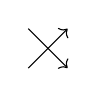
\begin{tikzpicture}[baseline={(0,0.15)}, scale=0.5]
                        \draw[->] (0.5,0) -- (1.5,1);
                        \draw[->] (0.5,1) -- (1.5,0);
                \end{tikzpicture}
                \,,\,
                \,\psi_2
                \right]
        }
        \QQ_a \PP_{b},
\end{equation}
defined in \cite[\S5.4]{gyenge2021heisenberg}. Here, it breaks 
\eqref{eqn-QP-word-iterative-procedure-step-1} into two summands. 
In one $\QQ_{a_1}$ is commuted past $\PP_{b_1}$, while in the other
$\QQ_{a_1}$ and $\PP_{b_1}$ annihilate each other and the rest 
is tensored by $\homm_{\basecat}(a_1, b_1)$:
\begin{equation}
\label{eqn-QP-word-iterative-procedure-step-2}
\begin{tikzcd}[row sep = 0.25cm]
\QQ_{a_n} \dots \QQ_{a_1} \PP_{b_1} \dots \PP_{b_m} 
\\
\QQ_{a_n} \dots \QQ_{a_2} \PP_{b_1}\QQ_{a_1} \PP_{b_2}  \dots \PP_{b_m} 
\oplus 
\QQ_{a_n} \dots \QQ_{a_2} \PP_{b_2}  \dots \PP_{b_m} \otimes
\homm_{\basecat}(a_1, b_1)
\ar{u}
\end{tikzcd}
\end{equation}

We now take each of the newly obtained summands and apply the same
procedure to them. We locate the rightmost $\QQ\PP$ subword, 
if one exists, and apply to it the homotopy equivalence 
\eqref{eq:dg-baby-Heisenberg-morphism}. This replaces the old summand
by two new ones, where the $\QQ\PP$ pair in question is commuted and
is annihilated, respectively. 
We repeat this until none of the summands contain a $\QQ\PP$ subword. 

The result is a homotopy equivalence into 
\eqref{eqn-QP-word-iterative-procedure-step-1} from a direct sum 
whose summands have form 
\begin{small}
\begin{equation}
\label{eqn-the-summands-of-sumPQcheck}
\PP_{b_1} \dots 
\widehat{\PP_{b_{j_1}}} \dots \widehat{\PP_{b_{j_k}}}
\dots \PP_{b_m}
\QQ_{a_n} \dots 
\widehat{\QQ_{a_{i_k}}} \dots \widehat{\QQ_{a_{i_1}}} 
\dots \QQ_{a_1}
\otimes \homm_{\basecat}(a_{i_1}, b_{j_{\sigma(1)}}) \otimes \dots \otimes 
\homm_{\basecat}(a_{i_k}, b_{j_{\sigma(k)}}). 
\end{equation}
\end{small}
where a hat indicates that we skip this element and where $\sigma \in S_k$. 
We obtain each summand by starting at 
\eqref{eqn-QP-word-iterative-procedure-step-1}, 
taking each $\QQ$ (from right to left) and starting to move it 
past all the $\PP$s. At each $\PP$ we choose whether to commute 
the $\QQ$ past it or to annihilate the $\QQ$ against it and start on 
the next $\QQ$. In \eqref{eqn-the-summands-of-sumPQcheck} the elements $\QQ_{a_{i_1}}$, \dots, $\QQ_{a_{i_k}}$ 
were annihilated against the elements $\PP_{b_{j_1}}$, \dots,
$\PP_{b_{j_k}}$ in the order specified by $\sigma$. 
The remaining $\QQ$s were succesfully commuted past all the $\PP$s. 
\end{Definition}


\begin{Example}
\label{exmpl-commutation-annihilation-procedure-for-n-equals-three}
Let $a_1, a_2, a_3, b_1, b_2, b_3 \in \basecat$. 
Write $(a_i,b_j)$ for $\homm_\basecat(a_i,b_j)$. For 
$$ \QQ_{a_3}\QQ_{a_2}\QQ_{a_1} \PP_{b_1}\PP_{b_2}\PP_{b_3} \in
\homm_{\hcat\basecat}(0,0) $$
the first few steps of
the commutation-annihilation procedure described above are 
\begin{tiny}
\begin{equation*}
\begin{tikzcd}[row sep = 0.25cm]
\QQ_{a_3}\QQ_{a_2}\QQ_{a_1} \PP_{b_1}\PP_{b_2}\PP_{b_3}
\\
\left(\QQ_{a_3}\QQ_{a_2}\PP_{b_1}\QQ_{a_1} \PP_{b_2}\PP_{b_3} \right)
\oplus 
\left(
\QQ_{a_3}\QQ_{a_2}\PP_{b_2}\PP_{b_3} \otimes (a_1, b_1)
\right)
\ar{u}
\\
\begin{matrix}
\left( 
\QQ_{a_3}\QQ_{a_2}\PP_{b_1}\PP_{b_2}\QQ_{a_1}\PP_{b_3} 
\right)
\oplus 
\left(
\QQ_{a_3}\QQ_{a_2}\PP_{b_1}\PP_{b_3} \otimes (a_1, b_2)
\right)
\oplus 
\left(
\QQ_{a_3}\PP_{b_2}\QQ_{a_2}\PP_{b_3} \otimes (a_1, b_1)
\right)
\oplus
\left( 
\QQ_{a_3}\PP_{b_3} \otimes (a_1, b_1) \otimes
(a_2, b_2)
\right)
\end{matrix}
\ar{u} 
\\
\begin{matrix}
\left( 
\QQ_{a_3}\QQ_{a_2}\PP_{b_1}\PP_{b_2}\PP_{b_3}\QQ_{a_1} 
\right)
\oplus
\left(
\QQ_{a_3}\QQ_{a_2}\PP_{b_1}\PP_{b_2} \otimes (a_1, b_3) 
\right)
\oplus 
\left(
\QQ_{a_3}\PP_{b_1}\QQ_{a_2}\PP_{b_3} \otimes (a_1, b_2)
\right)
\oplus 
\left(
\QQ_{a_3}\PP_{b_3} \otimes (a_1, b_2) \otimes
(a_2, b_1)
\right)
\oplus
\\
\oplus
\left(
\QQ_{a_3}\PP_{b_2}\PP_{b_3}\QQ_{a_2} \otimes (a_1, b_1)
\right)
\oplus
\left(
\QQ_{a_3}\PP_{b_2}\otimes (a_1, b_1) \otimes
(a_2, b_3)
\right)
\oplus
\left( 
\PP_{b_3}\QQ_{a_3} \otimes (a_1, b_1) \otimes
(a_2, b_2)
\right)
\oplus
\bigl( 
(a_1, b_1) \otimes (a_2, b_2)
\otimes (a_3, b_3)
\bigr)
\end{matrix}
\ar{u} 
\\
\begin{matrix}
\left( 
\QQ_{a_3}\PP_{b_1}\QQ_{a_2}\PP_{b_2}\PP_{b_3}\QQ_{a_1} 
\right)
\oplus
\left( 
\QQ_{a_3}\PP_{b_2}\PP_{b_3}\QQ_{a_1} \otimes (a_2, b_1)
\right)
\oplus
\left(
\QQ_{a_3}\PP_{b_1}\QQ_{a_2}\PP_{b_2} \otimes (a_1, b_3) 
\right)
\oplus
\left(
\QQ_{a_3}\PP_{b_2} \otimes (a_1, b_3) \otimes
(a_2, b_1)
\right)
\oplus 
\\
\oplus
\left(
\QQ_{a_3}\PP_{b_1}\PP_{b_3}\QQ_{a_2} \otimes (a_1, b_2)
\right)
\oplus 
\left(
\QQ_{a_3}\PP_{b_1} \otimes (a_1, b_2) \otimes
(a_2, b_3)
\right)
\oplus
\left(
\PP_{b_3}\QQ_{a_3} \otimes (a_1, b_2) \otimes
(a_2, b_1)
\right)
\oplus
\bigl(
(a_1, b_2) \otimes (a_2, b_1) \otimes (a_3, b_3)
\bigr)
\oplus
\\
\oplus
\left(
\PP_{b_2}\QQ_{a_3}\PP_{b_3}\QQ_{a_2} \otimes (a_1, b_1)
\right)
\oplus
\left(
\PP_{b_3}\QQ_{a_2} \otimes (a_1, b_1) \otimes
(a_3, b_2)
\right)
\oplus
\left(
\PP_{b_2}\QQ_{a_3}\otimes (a_1, b_1) \otimes
(a_2, b_3)
\right)
\oplus
\bigl(
(a_1, b_1) \otimes
(a_2, b_3) \otimes (a_3, b_2)
\bigr)
\oplus
\\
\oplus
\left( 
\PP_{b_3}\QQ_{a_3} \otimes (a_1, b_1) \otimes (a_2, b_2)
\right)
\oplus
\bigl( 
(a_1, b_1) \otimes (a_2, b_2) \otimes (a_3, b_3)
\bigr)
\end{matrix}
\ar{u}
% \\
% \begin{matrix}
% \left( 
% \QQ_{a_3}\PP_{b_1}\PP_{b_2}\QQ_{a_2}\PP_{b_3}\QQ_{a_1} 
% \right)
% \oplus
% \left( 
% \QQ_{a_3}\PP_{b_1}\PP_{b_3}\QQ_{a_1}  \otimes (a_2, b_2)
% \right)
% \oplus
% \left( 
% \PP_{b_2}\QQ_{a_3}\PP_{b_3}\QQ_{a_1} \otimes (a_2, b_1)
% \right)
% \oplus
% \left( 
% \PP_{b_3}\QQ_{a_1} \otimes (a_2, b_1) \otimes
% (a_3, b_2)
% \right)
% \oplus
% \\
% \oplus
% \left(
% \QQ_{a_3}\PP_{b_1}\PP_{b_2}\QQ_{a_2} \otimes (a_1, b_3) 
% \right)
% \oplus
% \left(
% \QQ_{a_3}\PP_{b_1} \otimes (a_1, b_3) \otimes (a_2, b_2)
% \right)
% \oplus
% \left(
% \PP_{b_2}\QQ_{a_3} \otimes (a_1, b_3) \otimes (a_2, b_1)
% \right)
% \oplus
% \bigl(
% (a_1, b_3) \otimes (a_2, b_1) \otimes (a_3, b_2)
% \bigr)
% \oplus 
% \\
% \oplus
% \left(
% \PP_{b_1}\QQ_{a_3}\PP_{b_3}\QQ_{a_2} \otimes (a_1, b_2)
% \right)
% \oplus 
% \left(
% \PP_{b_3}\QQ_{a_2} \otimes (a_1, b_2) \otimes (a_3, b_1)
% \right)
% \oplus 
% \left(
% \PP_{b_1}\QQ_{a_3} \otimes (a_1, b_2) \otimes (a_2, b_3)
% \right)
% \oplus 
% \bigl(
% (a_1, b_2) \otimes (a_2, b_3) \otimes (a_3, b_1)
% \bigr)
% \oplus 
% \\
% \oplus
% \left(
% \PP_{b_3}\QQ_{a_3} \otimes (a_1, b_2) \otimes (a_2, b_1)
% \right)
% \oplus
% \bigl(
% (a_1, b_2) \otimes (a_2, b_1) \otimes (a_3, b_3)
% \bigr)
% \oplus
% \left(
% \PP_{b_2}\PP_{b_3}\QQ_{a_3}\QQ_{a_2} \otimes (a_1, b_1)
% \right)
% \oplus
% \left(
% \PP_{b_2}\QQ_{a_2} \otimes (a_1, b_1) \otimes (a_3, b_3)
% \right)
% \oplus
% \\
% \oplus
% \left(
% \PP_{b_3}\QQ_{a_2} \otimes (a_1, b_1) \otimes (a_3, b_2)
% \right)
% \oplus
% \left(
% \PP_{b_2}\QQ_{a_3}\otimes (a_1, b_1) \otimes (a_2, b_3)
% \right)
% \oplus
% \bigl(
% (a_1, b_1) \otimes (a_2, b_3) \otimes (a_3, b_2)
% \bigr)
% \oplus
% \left( 
% \PP_{b_3}\QQ_{a_3} \otimes (a_1, b_1) \otimes (a_2, b_2)
% \right)
% \oplus
% \\
% \oplus
% \bigl(
% (a_1, b_1) \otimes (a_2, b_2) \otimes (a_3, b_3)
% \bigr)
% \end{matrix}
% \ar{u}
% \\
% \begin{matrix}
% \left( 
% \QQ_{a_3}\PP_{b_1}\PP_{b_2}\PP_{b_3}\QQ_{a_2}\QQ_{a_1} 
% \right)
% \oplus
% \left( 
% \QQ_{a_3}\PP_{b_1}\PP_{b_2}\QQ_{a_1} \otimes (a_2, b_3)
% \right)
% \oplus
% \left( 
% \PP_{b_1}\QQ_{a_3}\PP_{b_3}\QQ_{a_1}  \otimes (a_2, b_2)
% \right)
% \oplus
% \left( 
% \PP_{b_3}\QQ_{a_1}  \otimes (a_2, b_2) \otimes (a_3, b_1)
% \right)
% \oplus
% \\
% \oplus
% \left( 
% \PP_{b_2}\PP_{b_3}\QQ_{a_3}\QQ_{a_1} \otimes (a_2, b_1)
% \right)
% \oplus
% \left( 
% \PP_{b_2}\QQ_{a_1} \otimes (a_2, b_1) \otimes (a_3,b_3)
% \right)
% \oplus
% \left( 
% \PP_{b_3}\QQ_{a_1} \otimes (a_2, b_1) \otimes (a_3, b_2)
% \right)
% \oplus
% \left(
% \PP_{b_1}\QQ_{a_3}\PP_{b_2}\QQ_{a_2} \otimes (a_1, b_3) 
% \right)
% \oplus
% \\
% \oplus
% \left(
% \PP_{b_2}\QQ_{a_2} \otimes (a_1, b_3) \otimes (a_3, b_1)
% \right)
% \oplus
% \left(
% \PP_{b_1}\QQ_{a_3} \otimes (a_1, b_3) \otimes (a_2, b_2)
% \right)
% \oplus
% \bigl(
% (a_1, b_3) \otimes (a_2, b_2) \otimes (a_3, b_1)
% \bigr)
% \oplus
% \left(
% \PP_{b_2}\QQ_{a_3} \otimes (a_1, b_3) \otimes (a_2, b_1)
% \right)
% \oplus
% \\
% \oplus
% \bigl(
% (a_1, b_3) \otimes (a_2, b_1) \otimes (a_3, b_2)
% \bigr)
% \oplus 
% \left(
% \PP_{b_1}\PP_{b_3}\QQ_{a_3}\QQ_{a_2} \otimes (a_1, b_2)
% \right)
% \oplus 
% \left(
% \PP_{b_1}\QQ_{a_2} \otimes (a_1, b_2) \otimes (a_3, b_3)
% \right)
% \oplus
% \left(
% \PP_{b_3}\QQ_{a_2} \otimes (a_1, b_2) \otimes (a_3, b_1)
% \right)
% \oplus 
% \\
% \oplus
% \left(
% \PP_{b_1}\QQ_{a_3} \otimes (a_1, b_2) \otimes (a_2, b_3)
% \right)
% \oplus 
% \bigl(
% (a_1, b_2) \otimes (a_2, b_3) \otimes (a_3, b_1)
% \bigr)
% \oplus 
% \left(
% \PP_{b_3}\QQ_{a_3} \otimes (a_1, b_2) \otimes (a_2, b_1)
% \right)
% \oplus
% \bigl(
% (a_1, b_2) \otimes (a_2, b_1) \otimes (a_3, b_3)
% \bigr)
% \oplus
% \\
% \oplus
% \left(
% \PP_{b_2}\PP_{b_3}\QQ_{a_3}\QQ_{a_2} \otimes (a_1, b_1)
% \right)
% \oplus
% \left(
% \PP_{b_2}\QQ_{a_2} \otimes (a_1, b_1) \otimes (a_3, b_3)
% \right)
% \oplus
% \left(
% \PP_{b_3}\QQ_{a_2} \otimes (a_1, b_1) \otimes (a_3, b_2)
% \right)
% \oplus
% \left(
% \PP_{b_2}\QQ_{a_3}\otimes (a_1, b_1) \otimes (a_2, b_3)
% \right)
% \oplus
% \\
% \oplus
% \bigl(
% (a_1, b_1) \otimes (a_2, b_3) \otimes (a_3, b_2)
% \bigr)
% \oplus
% \left( 
% \PP_{b_3}\QQ_{a_3} \otimes (a_1, b_1) \otimes (a_2, b_2)
% \right)
% \oplus
% \bigl( 
% (a_1, b_1) \otimes (a_2, b_2) \otimes (a_3, b_3)
% \bigr)
% \end{matrix}
% \ar{u}
% \\
% \begin{matrix}
% \left( 
% \PP_{b_1}\QQ_{a_3}\PP_{b_2}\PP_{b_3}\QQ_{a_2}\QQ_{a_1} 
% \right)
% \oplus
% \left( 
% \PP_{b_2}\PP_{b_3}\QQ_{a_2}\QQ_{a_1} \otimes (a_3, b_1)
% \right)
% \oplus
% \left( 
% \PP_{b_1}\QQ_{a_3}\PP_{b_2}\QQ_{a_1} \otimes (a_2, b_3)
% \right)
% \oplus
% \left( 
% \PP_{b_2}\QQ_{a_1} \otimes (a_2, b_3) \otimes (a_3, b_1)
% \right)
% \oplus
% \\
% \oplus
% \left( 
% \PP_{b_1}\PP_{b_3}\QQ_{a_3}\QQ_{a_1}  \otimes (a_2, b_2)
% \right)
% \oplus
% \left( 
% \PP_{b_1}\QQ_{a_1}  \otimes (a_2, b_2) \otimes (a_3, b_3)
% \right)
% \oplus
% \left( 
% \PP_{b_3}\QQ_{a_1}  \otimes (a_2, b_2) \otimes (a_3, b_1)
% \right)
% \oplus
% \left( 
% \PP_{b_2}\PP_{b_3}\QQ_{a_3}\QQ_{a_1} \otimes (a_2, b_1)
% \right)
% \oplus
% \\
% \oplus
% \left( 
% \PP_{b_2}\QQ_{a_1} \otimes (a_2, b_1) \otimes (a_3,b_3)
% \right)
% \oplus
% \left( 
% \PP_{b_3}\QQ_{a_1} \otimes (a_2, b_1) \otimes (a_3, b_2)
% \right)
% \oplus
% \left(
% \PP_{b_1}\PP_{b_2}\QQ_{a_3}\QQ_{a_2} \otimes (a_1, b_3) 
% \right)
% \oplus
% \left(
% \PP_{b_1}\QQ_{a_2} \otimes (a_1, b_3) \otimes (a_3, b_2)
% \right)
% \oplus
% \\
% \oplus
% \left(
% \PP_{b_2}\QQ_{a_2} \otimes (a_1, b_3) \otimes (a_3, b_1)
% \right)
% \oplus
% \left(
% \PP_{b_1}\QQ_{a_3} \otimes (a_1, b_3) \otimes (a_2, b_2)
% \right)
% \oplus
% \bigl(
% (a_1, b_3) \otimes (a_2, b_2) \otimes (a_3,b_1)
% \bigr)
% \oplus
% \left(
% \PP_{b_2}\QQ_{a_3} \otimes (a_1, b_3) \otimes (a_2, b_1)
% \right)
% \oplus
% \\
% \oplus
% \bigl(
% (a_1, b_3) \otimes (a_2, b_1) \otimes (a_3, b_2)
% \bigr)
% \oplus 
% \left(
% \PP_{b_1}\PP_{b_3}\QQ_{a_3}\QQ_{a_2} \otimes (a_1, b_2)
% \right)
% \oplus
% \left(
% \PP_{b_1}\QQ_{a_2} \otimes (a_1, b_2) \otimes (a_3, b_3)
% \right)
% \oplus
% \left(
% \PP_{b_3}\QQ_{a_2} \otimes (a_1, b_2) \otimes (a_3, b_1)
% \right)
% \oplus 
% \\
% \oplus
% \left(
% \PP_{b_1}\QQ_{a_3} \otimes (a_1, b_2) \otimes (a_2, b_3)
% \right)
% \oplus
% \bigl(
% (a_1, b_2) \otimes (a_2, b_3) \otimes (a_3, b_1)
% \bigr)
% \oplus 
% \left(
% \PP_{b_3}\QQ_{a_3} \otimes (a_1, b_2) \otimes (a_2, b_1)
% \right)
% \oplus
% \bigl(
% (a_1, b_2) \otimes (a_2, b_1) \otimes (a_3, b_3)
% \bigr)
% \oplus
% \\
% \oplus
% \left(
% \PP_{b_2}\PP_{b_3}\QQ_{a_3}\QQ_{a_2} \otimes (a_1, b_1)
% \right)
% \oplus
% \left(
% \PP_{b_2}\QQ_{a_2} \otimes (a_1, b_1) \otimes (a_3, b_3)
% \right)
% \oplus
% \left(
% \PP_{b_3}\QQ_{a_2} \otimes (a_1, b_1) \otimes (a_3, b_2)
% \right)
% \oplus
% \left(
% \PP_{b_2}\QQ_{a_3}\otimes (a_1, b_1) \otimes (a_2, b_3)
% \right)
% \oplus
% \\
% \oplus
% \bigl(
% (a_1, b_1) \otimes (a_2, b_3) \otimes (a_3, b_2)
% \bigr)
% \oplus
% \left( 
% \PP_{b_3}\QQ_{a_3} \otimes (a_1, b_1) \otimes (a_2, b_2)
% \right)
% \oplus
% \bigl( 
% (a_1, b_1) \otimes (a_2, b_2) \otimes (a_3, b_3)
% \bigr)
% \end{matrix}
% \ar{u}
% \\
% \begin{matrix}
% \left( 
% \PP_{b_1}\PP_{b_2}\QQ_{a_3}\PP_{b_3}\QQ_{a_2}\QQ_{a_1} 
% \right)
% \oplus
% \left( 
% \PP_{b_1}\PP_{b_3}\QQ_{a_2}\QQ_{a_1} \otimes (a_3, b_2)
% \right)
% \oplus
% \left( 
% \PP_{b_2}\PP_{b_3}\QQ_{a_2}\QQ_{a_1} \otimes (a_3, b_1)
% \right)
% \oplus
% \left( 
% \PP_{b_1}\PP_{b_2}\QQ_{a_3}\QQ_{a_1} \otimes (a_2, b_3)
% \right)
% \oplus
% \\
% \oplus
% \left( 
% \PP_{b_1}\QQ_{a_1} \otimes (a_2, b_3) \otimes (a_3,b_2)
% \right)
% \oplus
% \left( 
% \PP_{b_2}\QQ_{a_1} \otimes (a_2, b_3) \otimes (a_3, b_1)
% \right)
% \oplus
% \left( 
% \PP_{b_1}\PP_{b_3}\QQ_{a_3}\QQ_{a_1}  \otimes (a_2, b_2)
% \right)
% \oplus
% \left( 
% \PP_{b_1}\QQ_{a_1}  \otimes (a_2, b_2) \otimes (a_3, b_3)
% \right)
% \oplus
% \\
% \oplus
% \left( 
% \PP_{b_3}\QQ_{a_1}  \otimes (a_2, b_2) \otimes (a_3, b_1)
% \right)
% \oplus
% \left( 
% \PP_{b_2}\PP_{b_3}\QQ_{a_3}\QQ_{a_1} \otimes (a_2, b_1)
% \right)
% \oplus
% \left( 
% \PP_{b_2}\QQ_{a_1} \otimes (a_2, b_1) \otimes (a_3,b_3)
% \right)
% \oplus
% \left( 
% \PP_{b_3}\QQ_{a_1} \otimes (a_2, b_1) \otimes (a_3, b_2)
% \right)
% \oplus
% \\
% \oplus
% \left(
% \PP_{b_1}\PP_{b_2}\QQ_{a_3}\QQ_{a_2} \otimes (a_1, b_3) 
% \right)
% \oplus
% \left(
% \PP_{b_1}\QQ_{a_2} \otimes (a_1, b_3) \otimes (a_3, b_2)
% \right)
% \oplus
% \left(
% \PP_{b_2}\QQ_{a_2} \otimes (a_1, b_3) \otimes (a_3, b_1)
% \right)
% \oplus
% \left(
% \PP_{b_1}\QQ_{a_3} \otimes (a_1, b_3) \otimes (a_2, b_2)
% \right)
% \oplus
% \\
% \oplus
% \bigl(
% (a_1, b_3) \otimes (a_2, b_2) \otimes (a_3,b_1)
% \bigr)
% \oplus
% \left(
% \PP_{b_2}\QQ_{a_3} \otimes (a_1, b_3) \otimes (a_2, b_1)
% \right)
% \oplus
% \bigl(
% (a_1, b_3) \otimes (a_2, b_1) \otimes (a_3, b_2)
% \bigr)
% \oplus 
% \left(
% \PP_{b_1}\PP_{b_3}\QQ_{a_3}\QQ_{a_2} \otimes (a_1, b_2)
% \right)
% \oplus
% \\
% \oplus
% \left(
% \PP_{b_1}\QQ_{a_2} \otimes (a_1, b_2) \otimes (a_3, b_3)
% \right)
% \oplus
% \left(
% \PP_{b_3}\QQ_{a_2} \otimes (a_1, b_2) \otimes (a_3, b_1)
% \right)
% \oplus
% \left(
% \PP_{b_1}\QQ_{a_3} \otimes (a_1, b_2) \otimes (a_2, b_3)
% \right)
% \oplus
% \bigl(
% (a_1, b_2) \otimes (a_2, b_3) \otimes (a_3, b_1)
% \bigr)
% \oplus 
% \\
% \oplus
% \left(
% \PP_{b_3}\QQ_{a_3} \otimes (a_1, b_2) \otimes (a_2, b_1)
% \right)
% \oplus
% \bigl(
% (a_1, b_2) \otimes (a_2, b_1) \otimes (a_3, b_3)
% \bigr)
% \oplus
% \left(
% \PP_{b_2}\PP_{b_3}\QQ_{a_3}\QQ_{a_2} \otimes (a_1, b_1)
% \right)
% \oplus
% \left(
% \PP_{b_2}\QQ_{a_2} \otimes (a_1, b_1) \otimes (a_3, b_3)
% \right)
% \oplus
% \\
% \oplus
% \left(
% \PP_{b_3}\QQ_{a_2} \otimes (a_1, b_1) \otimes (a_3, b_2)
% \right)
% \oplus
% \left(
% \PP_{b_2}\QQ_{a_3}\otimes (a_1, b_1) \otimes (a_2, b_3)
% \right)
% \oplus
% \bigl(
% (a_1, b_1) \otimes (a_2, b_3) \otimes (a_3, b_2)
% \bigr)
% \oplus
% \left( 
% \PP_{b_3}\QQ_{a_3} \otimes (a_1, b_1) \otimes (a_2, b_2)
% \right)
% \oplus
% \\
% \oplus
% \bigl( 
% (a_1, b_1) \otimes (a_2, b_2) \otimes (a_3, b_3)
% \bigr)
% \end{matrix}
% \ar{u}
% \\
% \begin{matrix}
% \left( 
% \PP_{b_1}\PP_{b_2}\PP_{b_3}\QQ_{a_3}\QQ_{a_2}\QQ_{a_1} 
% \right)
% \oplus
% \left( 
% \PP_{b_1}\PP_{b_2}\QQ_{a_2}\QQ_{a_1} \otimes (a_3, b_3)
% \right)
% \oplus
% \left( 
% \PP_{b_1}\PP_{b_3}\QQ_{a_2}\QQ_{a_1} \otimes (a_3, b_2)
% \right)
% \oplus
% \left( 
% \PP_{b_2}\PP_{b_3}\QQ_{a_2}\QQ_{a_1} \otimes (a_3, b_1)
% \right)
% \oplus
% \\
% \oplus
% \left( 
% \PP_{b_1}\PP_{b_2}\QQ_{a_3}\QQ_{a_1} \otimes (a_2, b_3)
% \right)
% \oplus
% \left( 
% \PP_{b_1}\QQ_{a_1} \otimes (a_2, b_3) \otimes (a_3,b_2)
% \right)
% \oplus
% \left( 
% \PP_{b_2}\QQ_{a_1} \otimes (a_2, b_3) \otimes (a_3, b_1)
% \right)
% \oplus
% \left( 
% \PP_{b_1}\PP_{b_3}\QQ_{a_3}\QQ_{a_1}  \otimes (a_2, b_2)
% \right)
% \oplus
% \\
% \oplus
% \left( 
% \PP_{b_1}\QQ_{a_1}  \otimes (a_2, b_2) \otimes (a_3, b_3)
% \right)
% \oplus
% \left( 
% \PP_{b_3}\QQ_{a_1}  \otimes (a_2, b_2) \otimes (a_3, b_1)
% \right)
% \oplus
% \left( 
% \PP_{b_2}\PP_{b_3}\QQ_{a_3}\QQ_{a_1} \otimes (a_2, b_1)
% \right)
% \oplus
% \left( 
% \PP_{b_2}\QQ_{a_1} \otimes (a_2, b_1) \otimes (a_3,b_3)
% \right)
% \oplus
% \\
% \oplus
% \left( 
% \PP_{b_3}\QQ_{a_1} \otimes (a_2, b_1) \otimes (a_3, b_2)
% \right)
% \oplus
% \left(
% \PP_{b_1}\PP_{b_2}\QQ_{a_3}\QQ_{a_2} \otimes (a_1, b_3) 
% \right)
% \oplus
% \left(
% \PP_{b_1}\QQ_{a_2} \otimes (a_1, b_3) \otimes (a_3, b_2)
% \right)
% \oplus
% \left(
% \PP_{b_2}\QQ_{a_2} \otimes (a_1, b_3) \otimes (a_3, b_1)
% \right)
% \oplus
% \\
% \oplus
% \left(
% \PP_{b_1}\QQ_{a_3} \otimes (a_1, b_3) \otimes (a_2, b_2)
% \right)
% \oplus
% \bigl(
% (a_1, b_3) \otimes (a_2, b_2) \otimes (a_3,b_1)
% \bigr)
% \oplus
% \left(
% \PP_{b_2}\QQ_{a_3} \otimes (a_1, b_3) \otimes (a_2, b_1)
% \right)
% \oplus
% \bigl(
% (a_1, b_3) \otimes (a_2, b_1) \otimes (a_3, b_2)
% \bigr)
% \oplus 
% \\
% \oplus
% \left(
% \PP_{b_1}\PP_{b_3}\QQ_{a_3}\QQ_{a_2} \otimes (a_1, b_2)
% \right)
% \oplus
% \left(
% \PP_{b_1}\QQ_{a_2} \otimes (a_1, b_2) \otimes (a_3, b_3)
% \right)
% \oplus
% \left(
% \PP_{b_3}\QQ_{a_2} \otimes (a_1, b_2) \otimes (a_3, b_1)
% \right)
% \oplus
% \left(
% \PP_{b_1}\QQ_{a_3} \otimes (a_1, b_2) \otimes (a_2, b_3)
% \right)
% \oplus
% \\
% \oplus
% \bigl(
% (a_1, b_2) \otimes (a_2, b_3) \otimes (a_3, b_1)
% \bigr)
% \oplus 
% \left(
% \PP_{b_3}\QQ_{a_3} \otimes (a_1, b_2) \otimes (a_2, b_1)
% \right)
% \oplus
% \bigl(
% (a_1, b_2) \otimes (a_2, b_1) \otimes (a_3, b_3)
% \bigr)
% \oplus
% \left(
% \PP_{b_2}\PP_{b_3}\QQ_{a_3}\QQ_{a_2} \otimes (a_1, b_1)
% \right)
% \oplus
% \\
% \oplus
% \left(
% \PP_{b_2}\QQ_{a_2} \otimes (a_1, b_1) \otimes (a_3, b_3)
% \right)
% \oplus
% \left(
% \PP_{b_3}\QQ_{a_2} \otimes (a_1, b_1) \otimes (a_3, b_2)
% \right)
% \oplus
% \left(
% \PP_{b_2}\QQ_{a_3}\otimes (a_1, b_1) \otimes (a_2, b_3)
% \right)
% \oplus
% \bigl(
% (a_1, b_1) \otimes (a_2, b_3) \otimes (a_3, b_2)
% \bigr)
% \oplus
% \\
% \oplus
% \left( 
% \PP_{b_3}\QQ_{a_3} \otimes (a_1, b_1) \otimes (a_2, b_2)
% \right)
% \oplus
% \bigl( 
% (a_1, b_1) \otimes (a_2, b_2) \otimes (a_3, b_3)
% \bigr)
% \end{matrix}
% \ar{u}
\end{tikzcd}
\end{equation*}
\end{tiny}

Its result is the direct sum whose summands, grouped by 
the number of annihilations, are:
\begin{enumerate}
\item $\;\;\;\PP_{b_1}\PP_{b_2}\PP_{b_3}\QQ_{a_3}\QQ_{a_2}\QQ_{a_1}$, 
\item 
$\;\;\;\bigl(
\PP_{b_2}\PP_{b_3}\QQ_{a_3}\QQ_{a_2} \otimes (a_1, b_1)
\bigr)
\oplus 
\bigl(
\PP_{b_1}\PP_{b_3}\QQ_{a_3}\QQ_{a_2} \otimes (a_1, b_2)
\bigr)
\oplus 
\bigl(
\PP_{b_1}\PP_{b_2}\QQ_{a_3}\QQ_{a_2} \otimes (a_1, b_3)
\bigr)
\oplus$ \\
$\oplus 
\bigl(
\PP_{b_2}\PP_{b_3}\QQ_{a_3}\QQ_{a_1} \otimes (a_2, b_1)
\bigr)
\oplus 
\bigl(
\PP_{b_1}\PP_{b_3}\QQ_{a_3}\QQ_{a_1} \otimes (a_2, b_2)
\bigr)
\oplus 
\bigl(
\PP_{b_1}\PP_{b_2}\QQ_{a_3}\QQ_{a_1} \otimes (a_2, b_3)
\bigr)
\oplus
$\\
$
\oplus
\bigl(
\PP_{b_2}\PP_{b_3}\QQ_{a_2}\QQ_{a_1} \otimes (a_3, b_1)
\bigr)
\oplus
\bigl(
\PP_{b_1}\PP_{b_3}\QQ_{a_2}\QQ_{a_1} \otimes (a_3, b_2)
\bigr)
\oplus
\bigl(
\PP_{b_1}\PP_{b_2}\QQ_{a_2}\QQ_{a_1} \otimes (a_3, b_3),
\bigr)
$ 

\item 
$\;\;\;\bigl
(\PP_{b_3}\QQ_{a_3} \otimes (a_1, b_1) \otimes (a_2, b_2)
\bigr)
\oplus 
\bigl(
\PP_{b_2}\QQ_{a_3} \otimes (a_1, b_1) \otimes (a_2, b_3)
\bigr)
\oplus 
\bigl(
\PP_{b_3}\QQ_{a_2} \otimes (a_1, b_1) \otimes (a_3, b_2)
\bigr)
\oplus$ \\
$\oplus 
\bigl(
\PP_{b_2}\QQ_{a_2} \otimes (a_1, b_1) \otimes (a_3, b_3)
\bigr)
\oplus 
\bigl(
\PP_{b_3}\QQ_{a_3} \otimes (a_1, b_2) \otimes (a_2, b_1)
\oplus 
\bigl(
\PP_{b_1}\QQ_{a_3} \otimes (a_1, b_2) \otimes (a_2, b_3)
\bigr)
\oplus$ \\
$\oplus 
\bigl(
\PP_{b_3}\QQ_{a_2} \otimes (a_1, b_2) \otimes (a_3, b_1)
\bigr)
\oplus 
\bigl(
\PP_{b_1}\QQ_{a_2} \otimes (a_1, b_2) \otimes (a_3, b_3)
\bigr)
\oplus 
\bigl(
\PP_{b_2}\QQ_{a_3} \otimes (a_1, b_3) \otimes (a_2, b_1)
\bigr)
\oplus$ \\
$\oplus 
\bigl(
\PP_{b_1}\QQ_{a_3} \otimes (a_1, b_3) \otimes (a_2, b_2)
\bigr)
\oplus 
\bigl(
\PP_{b_2}\QQ_{a_2} \otimes (a_1, b_3) \otimes (a_3, b_1)
\bigr)
\oplus 
\bigl(
\PP_{b_1}\QQ_{a_2} \otimes (a_1, b_3) \otimes (a_3, b_2)
\bigr)
\oplus$ \\
$\oplus 
\bigl(
\PP_{b_3}\QQ_{a_1} \otimes (a_2, b_1) \otimes (a_3, b_2)
\bigr)
\oplus 
\bigl(
\PP_{b_2}\QQ_{a_1} \otimes (a_2, b_1) \otimes (a_3, b_3)
\bigr)
\oplus 
\bigl(
\PP_{b_3}\QQ_{a_1} \otimes (a_2, b_2) \otimes (a_3, b_1)
\bigr)
\oplus$ \\
$\oplus 
\bigl(
\PP_{b_1}\QQ_{a_1} \otimes (a_2, b_2) \otimes (a_3, b_3)
\bigr)
\oplus 
\bigl(
\PP_{b_2}\QQ_{a_1} \otimes (a_2, b_3) \otimes (a_3, b_1)
\bigr)
\oplus 
\bigl(
\PP_{b_1}\QQ_{a_1} \otimes (a_2, b_3) \otimes (a_3, b_2)
\bigr)$
\item 
$\;\;\; 
\bigl(
(a_1, b_1) \otimes (a_2, b_2) \otimes (a_3, b_3)
\bigr)
\oplus 
\bigl(
(a_1, b_1) \otimes (a_2, b_3) \otimes (a_3, b_2)
\bigr)
\oplus 
\bigl(
(a_1, b_2) \otimes (a_2, b_1) \otimes (a_3, b_3)
\bigr)
\oplus$ \\
$\oplus 
\bigl(
(a_1, b_2) \otimes (a_2, b_3) \otimes (a_3, b_2)
\bigr)
\oplus 
\bigl(
(a_1, b_3) \otimes (a_2, b_1) \otimes (a_3, b_2)
\bigr)
\oplus 
\bigl(
(a_1, b_3) \otimes (a_2, b_2) \otimes (a_3, b_1)
\bigr)
$. 
\end{enumerate}
\end{Example}

We now make this procedure functorial. We begin with the annihilation:
\begin{Definition}
\label{defn-annihilation-functor}
Let $n,m > 0$ and let $\min(n,m) \geq k \geq 0$. Define the DG functor
\begin{equation}
(\hat{k})\colon 
\sym^{n}\basecat^{\opp} \otimes \sym^{m}\basecat
\longrightarrow 
\hperf\left(
\sym^{n-k}\basecat^{\opp} \otimes \sym^{m-k}\basecat \right)
\end{equation}
as the composition 
\begin{align*}
\sym^{n}\basecat^{\opp} \otimes \sym^{m}\basecat
\xrightarrow{
\Res_{S_{n-k} \times S_{k} \times S_{m-k}}^{S_n \times S_m}
}
& \hperf \left(
\sym^{n-k}\basecat^{\opp} 
\otimes 
\left(\left((\basecat^{\opp})^{\otimes k} \otimes \basecat^{\otimes k}\right)
\rtimes S_k\right) 
\otimes 
\sym^{m-k}\basecat
\right)
\simeq 
\\
\simeq 
& \hperf \left(
\sym^{n-k}\basecat^{\opp} 
\otimes 
\sym^k(\basecat^{\opp} \otimes \basecat)
\otimes 
\sym^{m-k}\basecat
\right)
\xrightarrow{\homm_\basecat(-,-)}
\\
\rightarrow 
&
\hperf \left(
\sym^{n-k}\basecat^{\opp} 
\otimes 
\sym^k(\hperf \kk)
\otimes 
\sym^{m-k}\basecat
\right)
\xrightarrow{(-) \otimes \dots \otimes (-)}
\\
\rightarrow 
& \hperf \left(
\sym^{n-k}\basecat^{\opp} 
\otimes 
\hperf \kk
\otimes 
\sym^{m-k}\basecat
\right)
\simeq 
\\
\simeq 
&
\hperf \left(
\sym^{n-k}\basecat^{\opp} 
\otimes 
\sym^{m-k}\basecat
\right).
\end{align*}
The first composant
is the restriction of scalars functors induced by the group embedding 
$$ S_{n-k} \times S_{k} \times S_{m-k} \hookrightarrow 
S_{n-k} \times S_{k} \times S_{k} \times S_{m-k}
\hookrightarrow  S_{n} \times S_{m} $$
where $S_k$ embeds into $S_k \times S_k$ as $\sigma \mapsto (\iota
\sigma \iota, \sigma)$ with $\iota$  the order reversing involution 
$1 \dots n \mapsto n \dots 1$. 

The second composant is induced by the factor permuting isomorphism 
$$ \left(\basecat^{\opp}\right)^{\otimes k} \otimes \basecat^{\otimes k} 
\simeq (\basecat^{\opp} \otimes \basecat)^{\otimes k} $$
which sends $a_k \otimes \dots \otimes a_1 \otimes b_1 \otimes \dots
\otimes b_k$ to $a_1 \otimes b_1 \otimes 
\dots \otimes a_k \otimes b_k$. 

The third composant is induced by the functor 
$$ \homm_\basecat(-,-) \colon \basecat^{\opp} \otimes \basecat
\rightarrow \hperf \kk $$
which sends $a \otimes b \mapsto \homm_{\basecat}(a,b)$. 

The fourth composant is induced by the functor 
$$ 
(-) \otimes \dots \otimes (-) \colon 
\sym^k \hperf \kk \rightarrow \hperf \kk $$
which tensors $k$ complexes of $\kk$-modules together. 

The last composant is the isomorphism given by 
the restriction of scalars along the Yoneda embedding 
$\kk \rightarrow \hperf \kk$. 
\end{Definition}

\begin{Lemma}
\label{lemma-explicit-description-of-the-functor-hatk}
Let $n,m > 0$ and $\min(n,m) \geq k \geq 0$. Let
$a_1, \dots, a_n \in \basecat$ and $b_1, \dots, b_m \in \basecat$. 
Then
$$
(\hat{k})\left((a_n \otimes \dots \otimes a_1) \otimes (b_1 \otimes
\dots \otimes b_m)\right) \simeq
$$
\begin{equation}
\label{eqn-direct-sum-decomposition-of-hatk}
\bigoplus_{
\begin{smallmatrix}
1 \leq i_1 < \dots < i_k \leq n, \\
1 \leq j_1 < \dots < j_k \leq m, \\
\sigma \in S_k
\end{smallmatrix}
}
\begin{matrix}
(a_n \otimes \dots \widehat{a_{i_k}} \dots \widehat{a_{i_1}} \dots \otimes a_1) \otimes 
(b_1 \otimes \dots \widehat{b_{j_1}} \dots \widehat{b_{j_k}} \dots \otimes b_m) \otimes 
\\
\otimes \homm_{\basecat}(a_{i_1}, b_{j_{\sigma(1)}}) 
\otimes 
\dots 
\otimes 
\homm_{\basecat}(a_{i_k}, b_{j_{\sigma(k)}}). 
\end{matrix}
\end{equation}

Furthermore, let $\alpha_i \in \homm_\basecat(a'_i, a_i)$ for $1 \leq i \leq n$ and $\beta_j \in \homm_\basecat(b_j, b'_j)$ for $1 \leq j \leq m$. Then 
in terms of the direct sum decomposition  
\eqref{eqn-direct-sum-decomposition-of-hatk}
$$ (\hat{k})\bigl((\alpha_n \otimes \dots \otimes \alpha_1) \otimes (\beta_1 \otimes
\dots \otimes \beta_m)\bigr) $$
maps the summand indexed by 
$1 \leq i_1 < \dots < i_k \leq n $,
$1 \leq j_1 < \dots < j_k  \leq m$, 
and $\sigma \in S_k$ to the summand with the same index via the map 
$$ (\alpha_m \otimes \dots \widehat{\alpha_{i_k}} \dots \widehat{\alpha_{i_1}} \dots \otimes \alpha_1) \otimes 
(\beta_1 \otimes \dots \widehat{\beta_{j_{\sigma(1)}}} \dots \widehat{\beta_{j_{\sigma(k)}}} 
\dots \otimes \beta_m ) 
\otimes 
(\beta_{j_{\sigma(1)}} \circ \alpha_1) \otimes \dots \otimes (\beta_{j_{\sigma(k)}} \circ \alpha_k).   
$$

Similarly, let $\eta \in S_n$ and $\zeta \in S_m$. Then 
$$ (\hat{k})\bigl(\eta \otimes \zeta \bigr) $$
maps the summand indexed by $1 \leq i_1 < \dots < i_k \leq n$,
$1 \leq j_1 < \dots < j_k  \leq m$, and $\sigma \in S_k$ 
to the one indexed by 
$1 \leq \eta(i_{\tau^{-1}(1)}) < \dots < \eta(i_{\tau^{-1}(k)}) \leq n$, 
$1 \leq \zeta(j_{\upsilon^{-1}(1)}) < \dots <
\zeta(j_{\upsilon^{-1}(k)}) \leq m$, 
and $\upsilon \sigma \tau^{-1} \in S_k$ via the isomorphism
$$ \phi \otimes \tau \otimes \chi $$
where
\begin{itemize}
\item $\tau \in S_k$ reorders  
$\eta(i_1)$, \dots, $\eta(i_k)$ in the increasing order,
\item $\upsilon \in S_k$ reorders 
$\zeta(j_1)$, \dots, $\zeta(j_k)$ in the increasing order, 
\item $\phi \in S_{n-k}$ reorders 
$\eta(n) \dots \widehat{\eta(i_k)} \dots  \widehat{\eta(i_1)} \dots
\eta(1)$ 
in the decreasing order, 
\item $\chi \in S_{m-k}$ reorders
$\zeta(1) \dots \widehat{\zeta(j_1)} \dots  \widehat{\zeta(j_k)} \dots
\zeta(m)$ in the increasing order. 
\end{itemize}
\end{Lemma}
\begin{proof}
For any $p > q > 0$ the left cosets of 
$S_{p-q} \otimes S_q \hookrightarrow S_p$
are enumerated by the partitions of $\left\{1,\dots, p\right\}$ 
into $q$ and $p-q$ elements. This can be viewed as choices of
$1 \leq i_1 < \dots < i_q \leq p$ and as a representative of each coset 
we can take either of the permutations
$$ 1\dots p \mapsto 1\dots \widehat{i_1} \dots  \widehat{i_q} \dots p \;
i_1 \dots i_q, $$
$$ 1\dots p \mapsto p\dots \widehat{i_q} \dots  \widehat{i_1} \dots 1 \;
i_q \dots i_1. $$  
For any $p > 0$ the left cosets of 
$S_p \hookrightarrow S_p \times S_p$
with the embedding as in Definition \ref{defn-annihilation-functor} 
are enumerated by permutations $\sigma \in S_p$. As a representative
of each coset we can take $\id \times \sigma$ or $\sigma \times \id$.  

Hence the left cosets of 
$S_{n-k} \times S_{k} \times S_{m-k} \hookrightarrow  S_{n} \times S_{m}$
are given by choices of $1 \leq i_1 < \dots < i_k \leq n$, 
$1 \leq j_1 < \dots < j_k \leq m$, $\sigma \in S_k$. 
The coset corresponding to $(\underline{i}, \underline{j}, \sigma)$
has the representative 
\begin{equation}
\rho_{\underline{i}, \underline{j}, \sigma}
:= 
\text{ the product of }
\begin{cases}
1\dots n \mapsto n\dots \widehat{i_k} \dots  \widehat{i_1} \dots
1\; i_k \dots i_1 & \quad \in S_n, \\
1\dots m \mapsto j_{\sigma(1)}  \dots j_{\sigma(k)} 
\; 1\dots \widehat{j_1} \dots  \widehat{j_k} \dots m & \quad \in S_m. 
\end{cases}
\end{equation}

The group $S_n \times S_m$ acts on the set of left
cosets of $S_{n-k} \times S_{k} \times S_{m-k}$ by left
multiplication. On the coset representatives $\rho_{\underline{i},
\underline{j}, \sigma}$, for any 
$\eta \times \zeta \in S_n \times S_m$ we have 
$$ (\eta \times \zeta) \rho_{(\underline{i}, \underline{j}, \sigma)} = 
\rho_{(\eta(\underline{i}), \zeta(\underline{j}), \upsilon\sigma\tau^{-1})} 
(\phi \times \tau \times \chi)
\quad \quad \quad 
(\phi \times \tau \times \chi) \in S_{n-k} \times S_k \times S_{m-k}
$$
with $\tau$, $\upsilon$, $\phi$, and $\chi$ as above. 
By Lemma  
\ref{lemma-descripton-of-res-G-to-H-functor}
the first composant
$\Res_{S_{n-k} \times S_{k} \times S_{m-k}}^{S_n \times S_m}$ of
$(\hat{k})$ sends 
$$  (a_n \otimes \dots \otimes a_1) \otimes (b_1 \otimes \dots \otimes b_m) $$
to the direct sum of representable modules
$$ \bigoplus_{
\begin{smallmatrix}
1 \leq i_1 < \dots < i_k \leq n, \\
1 \leq j_1 < \dots < j_k \leq m, \\
\sigma \in S_k
\end{smallmatrix}
}
(a_n \otimes \dots \widehat{a_{i_k}} \dots \widehat{a_{i_1}} \dots
\otimes a_1) \otimes a_{i_k} \otimes \dots \otimes a_{i_1} \otimes 
b_{j_{\sigma(1)}} \otimes \dots \otimes b_{j_{\sigma(k)}} \otimes 
(b_1 \times \dots \widehat{b_{j_1}} \dots \widehat{b_{j_k}} \dots
\otimes b_m). 
$$

The second composant sends each summand to  
$$ 
(a_n \otimes \dots \widehat{a_{i_k}} \dots \widehat{a_{i_1}} \dots
\otimes a_1) \otimes (a_{i_1} \otimes b_{j_{\sigma(1)}}) 
\otimes \dots \otimes (a_{i_k} \otimes b_{j_{\sigma(k)}}) \otimes 
(b_1 \times \dots \widehat{b_{j_1}} \dots \widehat{b_{j_k}} \dots
\otimes b_m). 
$$
The third sends it further to  
$$
(a_n \otimes \dots \widehat{a_{i_k}} \dots \widehat{a_{i_1}} \dots
\otimes a_1) \otimes \homm_{\basecat}(a_{i_1}, b_{j_{\sigma(1)}}) 
\otimes \dots \otimes \homm_{\basecat}(a_{i_k}, b_{j_{\sigma(k)}}) 
\otimes (b_1 \otimes \dots \widehat{b_{j_1}} \dots \widehat{b_{j_k}} \dots
\otimes b_m). 
$$
The fourth views the factor
$$ \homm_{\basecat}(a_{i_1}, b_{j_{\sigma(1)}}) 
\otimes \dots \otimes \homm_{\basecat}(a_{i_k}, b_{j_{\sigma(k)}}) $$
as a representable $(\hperf \kk)$-module instead of a representable 
$\sym^k(\hperf \kk)$-module. Finally the fifth views it as a
perfect $\kk$-module instead of a representable $(\hperf \kk)$-module. 

The remaining assertions 
follow similarly by Lemma \ref{lemma-descripton-of-res-G-to-H-functor}. 
\end{proof}

We now define a $2$-functor corresponding to each group of summands 
with the same number of annihilations in the result of the
commutation-annihilation procedure of
Definition \ref{defn-commutation-annihilation-procedure}. 

\begin{Definition}
\label{defn-two-functor-PQhatk}
For any $k \geq 0$ define a $2$-functor 
\begin{equation}
\label{eqn-two-functor-PQhatk}
\Xi_{\PP\QQ}(\hat{k})\colon 
\bicat{Sym}_{{\basecat}^{\opp}} \otimes \bicat{Sym}_{\basecat}
\rightarrow 
\hcat\basecat \otimes \hcat\basecat
\rightarrow \hcat\basecat
\end{equation}
on objects to be the map $(n,m) \mapsto m - n$ for all $n,m \in \mathbb{Z}$
and on $1$-morphisms to be the functor
$$ \homm_{\bicat{Sym}_{{\basecat}^{\opp}} \otimes
\bicat{Sym}_{\basecat}}\bigl((r,s), (r+n, s+m)\bigr) \rightarrow 
\homm_{\hcat\basecat}\bigl(s-r, (s-r) + (m-n)\bigr) 
\quad \quad \forall\; r,s,n,m \in \mathbb{Z} $$
defined for $k > \min(n,m)$ to be zero and 
for $k \leq \min(n,m)$ to be the composition 
\begin{align*}
\sym^{n}\basecat^{\opp} \otimes \sym^{m}\basecat
\xrightarrow{(\hat{k})}
& \hperf\left(
\sym^{n-k}\basecat^{\opp} \otimes \sym^{m-k}\basecat \right)
\simeq 
\hperf\left( \sym^{n-k}\basecat^{\opp} \right) 
\otimes 
\hperf\left( \sym^{m-k}\basecat \right)\simeq
\\
\simeq 
& \hperf\left( \sym^{m-k}\basecat \right)
\otimes 
\hperf\left( \sym^{n-k}\basecat^{\opp} \right)
\xrightarrow{\Xi_\PP \circ_1 \Xi_\QQ}
\homm_{\hcat\basecat}\bigl(s-r,(s-r)+(m-n)\bigr). 
\end{align*}
\end{Definition}

We finally define the second functor \eqref{eqn-two-functors-SnSm-H}
which we show to be homotopy equivalent to $\Xi_{\QQ\PP}$:

\begin{Definition}
\label{defn-dg-functor-PQhatk}
Define the functor
\begin{equation}
\bigoplus \Xi_{\PP\QQ}(\hat{k})\colon
\sym^{n}\basecat^{\opp} \otimes \sym^{m}\basecat
\rightarrow 
\homm_{\hcat\basecat}(0,m-n)
\end{equation}
to be the action of the $2$-functor 
$\bigoplus_{k=0}^{\infty} \Xi_{PQ}(\hat{k})$
on the $1$-morphism category $\homm_{\bicat{Sym}_{{\basecat}^{\opp}}
\otimes \bicat{Sym}_{\basecat}}((0,0), (n,m))$. 
\end{Definition}

\begin{Corollary}
For any object
$$ (a_n \otimes \dots \otimes a_1) \otimes (b_1 \otimes \dots \otimes
b_m) \in \sym^{n}\basecat^{\opp} \otimes \sym^{m}\basecat $$
the $1$-morphism 
$$ 
\bigoplus \Xi_{\PP\QQ}(\hat{k})\bigl(
(a_n \otimes \dots \otimes a_1) \otimes (b_1 \otimes \dots \otimes
\bigr)
$$
is isomorphic to the result of the commutation-annihilation procedure
of Definition \ref{defn-commutation-annihilation-procedure} applied
to 
$$ 
\Xi_{\QQ\PP}
\bigl( (a_n \otimes \dots \otimes a_1) \otimes (b_1 \otimes \dots
\otimes b_n)
\bigr).
$$
\end{Corollary}
\begin{proof}
This follows from Lemma 
\ref{lemma-explicit-description-of-the-functor-hatk}
and the description of the summands of the result of the
commutation-annihilation procedure given in 
\eqref{eqn-the-summands-of-sumPQcheck}. 
\end{proof}

We need to show that the homotopy equivalence
given by the commutation-annihilation procedure 
$$ \bigoplus \Xi_{\PP\QQ}(\hat{k})\bigl(
(a_n \otimes \dots \otimes a_1) \otimes (b_1 \otimes \dots \otimes b_n
\bigr)
\xrightarrow{\sim}
\Xi_{QP}
\bigl( (a_n \otimes \dots \otimes a_1) \otimes (b_1 \otimes \dots
\otimes b_n)
\bigr)
$$ 
define a natural transformation 
$ \bigoplus \Xi_{\PP\QQ}(\hat{k}) \rightarrow \Xi_{\QQ\PP}$. 
First, we give a direct definition:
\begin{Definition}
\label{defn-natural-transformation-phi-termwise} 
Let 
$$ \underline{a} = (a_n \otimes \dots \otimes a_1) \in
\sym^{n}\basecat^{\opp}, $$
$$ \underline{b} = (b_1 \otimes \dots \otimes b_m) \in  
\otimes \sym^{m}\basecat. $$
Define a $2$-morphism in $\hcat\basecat$ 
\begin{equation}
\label{eqn-natural-transformation-phi-termwise} 
\phi\colon \bigoplus \Xi_{\PP\QQ}(\hat{k})\bigl(\underline{a} \otimes \underline{b} \bigr)
\longrightarrow 
\Xi_{\PP\QQ}\bigl(\underline{a} \otimes \underline{b}\bigr)
\end{equation}
by setting for 
$0 \leq k \leq \min(n,m)$, $1 \leq i_1 < \dots < i_k \leq n$, 
$1 \leq j_1 < \dots < j_k \leq m$, and $\sigma \in S_k$
the component of $\phi$ on the corresponding summand of 
$\Xi_{\PP\QQ}(\hat{k})\bigl(\underline{a} \otimes \underline{b} \bigr)$
to be the adjoint of the morphism
\begin{equation}
\label{eqn-the-adjoint-of-the-natural-transformation-phi}
\begin{tikzcd}[row sep=0.25cm]
\homm_{\basecat}(a_{i_1}, b_{j_{\sigma(1)}}) \otimes \dots \otimes 
\homm_{\basecat}(a_{i_k}, b_{j_{\sigma(k)}})
\ar{d}
\\
\homm_{\hcat\basecat}\left(
\PP_{b_1} \dots 
\widehat{\PP_{b_{j_\bullet}}} 
\dots \PP_{b_m}
\QQ_{a_n} \dots 
\widehat{\QQ_{a_{i_\bullet}}} 
\dots \QQ_{a_1}, \quad 
\QQ_{a_n} \dots \QQ_{a_1} \PP_{b_1} \dots \PP_{b_m}\right)
\end{tikzcd}
\end{equation}
which sends each $\gamma_1 \otimes \dots \otimes \gamma_k$
to the $2$-morphism in $\hcat\basecat$ 
defined by the following planar diagram:
\begin{enumerate}
\item First, draw the annihilation strands. Start at the top of
the diagram, and for each $1 \leq l \leq k$ draw a circular strand 
counterclockwise from $\QQ_{i_l}$ to $\PP_{j_{\sigma(l)}}$ and
decorate it by $\gamma_l$. Draw these
so that each annihilation strand dips below the previous one, i.e. 
the height of the $l$-th strand arc is less than that of the $(l+1)$-st
for all $1 \leq l < k$. 
\begin{center}
\includegraphics[width=0.45\textwidth]{Figures/figure-10a}
\end{center}
\item Next, begin drawing the commutation strands. From each of
the remaining $\QQ$s and $\PP$s draw a vertical line down to some
horizontal level line below all the annihilation strands. 
\begin{center}
\includegraphics[width=0.45\textwidth]{Figures/figure-10b}
\end{center}
\item Finish by starting at that level and joing the commutation strand  
of each $\QQ_{a_i}$ or $\PP_{b_j}$ at the top of the diagram
to the same $\QQ_{a_i}$ or $\PP_{b_j}$ at the bottom of the diagram in a
straight line. 
\begin{center}
\includegraphics[width=0.45\textwidth]{Figures/figure-10c}
\end{center}
\end{enumerate}
\end{Definition}

Denote the component of $\phi$ on each summand of 
$\Xi_{\PP\QQ}(\hat{k})\bigl(\underline{a} \otimes \underline{b} \bigr)$
by the same diagram as its adjoint
\eqref{eqn-the-adjoint-of-the-natural-transformation-phi} only
with each annihilation strand decorated 
by $(a_{i_l}, b_{j_{\sigma(l)}})$ instead of $\gamma_l$:
\begin{center}
\includegraphics[width=0.45\textwidth]{Figures/figure-11}
\end{center}

\begin{Proposition}
\label{prps-natural-transformation-phi-is-homotopy-equivalence}
For any 
$\underline{a} = (a_n \otimes \dots \otimes a_1) \in
\sym^{n}\basecat^{\opp}$ and 
$\underline{b} = (b_1 \otimes \dots \otimes b_m) \in  
\otimes \sym^{m}\basecat$, 
the $2$-morphism 
$\phi\colon \bigoplus \Xi_{\PP\QQ}(\hat{k})\bigl(\underline{a} \otimes \underline{b} \bigr)
\longrightarrow 
\Xi_{\QQ\PP}\bigl(\underline{a} \otimes \underline{b}\bigr)$
of Defn.~\ref{defn-natural-transformation-phi-termwise}
equals in $\hcat\basecat$ 
the one constructed by the commutation-annihilation procedure
of Defn.~\ref{defn-commutation-annihilation-procedure}. In 
particular, it is a homotopy equivalence. 
\end{Proposition}
\begin{proof}
This follows from the pitchfork and triple move relations 
in $\hcat\basecat$ \cite[Lemma 5.5]{gyenge2021heisenberg}. 

We can prove it separately for each summand of 
$\bigoplus \Xi_{\PP\QQ}(\hat{k})\bigl(\underline{a} \otimes \underline{b}
\bigr)$. For a given summand,
the commutation-annihilation procedure construct the following
$2$-morphism into 
$\Xi_{\QQ\PP}\bigl(\underline{a} \otimes \underline{b}\bigr)$. 
We begin at the top of the diagram at $\QQ_{a_1}$ and 
perform rightward crossings 
$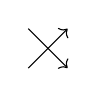
\begin{tikzpicture}[baseline={(0,0.15)}, scale=0.5]
\draw[->] (0.5,0) -- (1.5,1);
\draw[->] (0.5,1) -- (1.5,0);
\end{tikzpicture}$ until: 
\begin{itemize}
\item If the $\QQ_{a_1}$-strand is a commutation strand -- 
until it moves to the right of all $\PP$-strands, 
\item If the $\QQ_{a_1}$-strand is an annihilation strand -- 
until it reaches the $\PP_{b_j}$-strand it is paired with. 
The two strands are then terminated by a cup marked by $(a_1, b_j)$. 
\end{itemize}
We then repeat the same for $\QQ_{a_2}$, etc. 
\begin{equation*}
\begin{minipage}{0.35\textwidth}
\includegraphics[width=\textwidth]{Figures/figure-12a}
\end{minipage}
=
\begin{minipage}{0.45\textwidth}
\includegraphics[width=\textwidth]{Figures/figure-12b}
\end{minipage} 
\end{equation*}

If we take this planar diagram and consider all the annihilation strands
separately and all the commutation strands separately, then 
the two configurations match, possibly up to some pitchfork relations, 
the configurations of the annihilation and of the commutation strands 
in the planar diagram defining the corresponding component of 
the $2$-morphism $\phi$ of Definition 
\ref{defn-natural-transformation-phi-termwise}. 
\begin{equation*}
\begin{minipage}{0.45\textwidth}
\includegraphics[width=\textwidth]{Figures/figure-13a}
\end{minipage}
\;\;
\begin{minipage}{0.45\textwidth}
\includegraphics[width=\textwidth]{Figures/figure-13b}
\end{minipage} 
\end{equation*}

Now taking all the commutation strand crossings in the
commutation-annihilation planar diagram and using triple moves to
commute them downwards past all the annihilation strands produces the
planar diagram in the definition of $\phi$.
\begin{equation*}
\begin{minipage}{0.45\textwidth}
\includegraphics[width=\textwidth]{Figures/figure-14a}
\end{minipage}
=
\begin{minipage}{0.45\textwidth}
\includegraphics[width=\textwidth]{Figures/figure-14b}
\end{minipage} 
\end{equation*}
We conclude that the two planar diagrams define the same $2$-morphism 
in $\hcat\basecat$.  
\end{proof}

The following can be viewed as a functorial 
categorification of the PQ Heisenberg relation
\eqref{eq:vectheisrel3-graded}:

\begin{Theorem}
\label{theorem-functorial-categorification-of-the-PQ-Heisenberg-relation}
The $2$-morphisms $\phi$ of Definition 
\ref{defn-natural-transformation-phi-termwise}
define a DG natural transformation 
\begin{equation}
\label{eqn-functorial-categorification-of-the-PQ-Heisenberg-relation}
\phi\colon \bigoplus \Xi_{\PP\QQ}(\hat{k})
\longrightarrow 
\Xi_{\QQ\PP}
\end{equation}
of DG functors
$\sym^{n}\basecat^{\opp} \otimes \sym^{m}\basecat \rightarrow 
\homm_{\hcat\basecat}(0,m-n)$. By Prps.~\ref{prps-natural-transformation-phi-is-homotopy-equivalence}, 
$\phi$ is a homotopy equivalence. 
\end{Theorem}


A non-functorial categorification of the Heisenberg relation 
appeared in \cite[Theorem 6.3]{gyenge2021heisenberg}. However, it relates
the symmetrised elements $\PP_a^{(n)}$ and $\QQ_b^{(m)}$ and
as these are not functorial in $a,b \in \basecat$ for $n,m > 1$, 
there was little hope of making it functorial directly. Instead, 
we used its basic case $n = m = 1$ to iteratively construct
the present, functorial categorification
\eqref{eqn-functorial-categorification-of-the-PQ-Heisenberg-relation}. 
It is clear that applying  
\eqref{eqn-functorial-categorification-of-the-PQ-Heisenberg-relation}
to the product of the symmetrised powers 
$a^{(n)} \in \sym^{n}\basecat^{\opp} $ and $b^{(m)} \in
\sym^{m}\basecat$, defined via the twisted complexes analogous
to those defining $\PP_a^{(n)}$ and $\QQ_b^{(m)}$ in 
\cite[Definition 6.2]{gyenge2021heisenberg}, recovers the
non-functorial categorification of \cite[Theorem 6.3]{gyenge2021heisenberg}. 

\begin{proof}[Proof of Theorem
\ref{theorem-functorial-categorification-of-the-PQ-Heisenberg-relation}]

We need to show that for all 
$$ \underline{a} = (a_n \otimes \dots \otimes a_1) \text{ and }
\underline{a}' = (a'_n \otimes \dots \otimes a'_1) \in
\sym^{n}\basecat^{\opp}, $$
$$ \underline{b} = (b_1 \otimes \dots \otimes b_m) \text{ and }
\underline{b'} = (b'_1 \otimes \dots \otimes b'_m)
 \in \otimes \sym^{m}\basecat $$
and each morphism 
\begin{equation}
\label{eqn-morphisms-in-S^n-basecatopp-S^m-basecat-for-functoriality-of-phi}
\underline{\alpha} \otimes \underline{\beta} 
\colon \underline{a} \otimes \underline{b}
\rightarrow \underline{a}' \otimes \underline{b}'
\quad \quad \text{ in } \sym^{n}\basecat^{\opp} \otimes
\sym^{m}\basecat
\end{equation}
the corresponding square commutes in
$\homm_{\hcat\basecat}(0,m-n)$:
\begin{equation}
\label{eqn-commutative-square-for-the-functoriality-of-phi}
\begin{tikzcd}[column sep = 3cm]
\Xi_{\QQ\PP}\left(\underline{a} \otimes \underline{b}\right)
\ar{r}{\Xi_{\QQ\PP}(\underline{\alpha} \otimes \underline{\beta})}
&
\Xi_{\QQ\PP}\left(\underline{a}' \otimes \underline{b}' \right)
\\
\bigoplus \Xi_{\PP\QQ}(\hat{k})\left(\underline{a} \otimes \underline{b}\right)
\ar{r}{\bigoplus \Xi_{\PP\QQ}(\hat{k})(\underline{\alpha} \otimes \underline{\beta})}
\ar{u}{\phi_{\underline{a} \otimes \underline{b}}}
&
\bigoplus \Xi_{\PP\QQ}(\hat{k})\left(\underline{a}' \otimes
\underline{b}'\right).
\ar{u}{\phi_{\underline{a}' \otimes \underline{b}'}}
\end{tikzcd}
\end{equation}
The action of $\Xi_{\QQ\PP}$ on the 
morphism spaces of $\sym^{n}\basecat^{\opp} \otimes
\sym^{m}\basecat$ is clear. The functor $\Xi_{\PP\QQ}(\hat{k})$
is defined in terms of the functor $(\hat{k})$ whose
definition is more involved. However, the action of $(\hat{k})$
on the morphism spaces of $\sym^{n}\basecat^{\opp} \otimes
\sym^{m}\basecat$ is described explicitly by Lemma
\ref{lemma-explicit-description-of-the-functor-hatk}. We thus
prove the functoriality of $\phi$ by explicitly verifying for 
each generating morphism of 
$\sym^{n}\basecat^{\opp} \otimes \sym^{m}\basecat$ that 
\eqref{eqn-commutative-square-for-the-functoriality-of-phi}
commutes
in $\homm_{\hcat\basecat}(0,m-n)$. This reduces, once more,
to applying the pitchfork and triple move relations
\cite[Lemma 5.5]{gyenge2021heisenberg} and the dot sliding 
relations \cite[Lemma 5.4]{gyenge2021heisenberg}. 

Indeed, it suffices to prove that
\eqref{eqn-commutative-square-for-the-functoriality-of-phi}
commutes for each direct summand of $\bigoplus
\Xi_{\PP\QQ}(\hat{k})\left(\underline{a} \otimes \underline{b}\right)$. 
Fix $0 \leq k \leq \min(n,m)$. 
By Lemma \ref{lemma-explicit-description-of-the-functor-hatk}, 
each $\Xi_{\PP\QQ}(\hat{k})\left(\underline{a} \otimes
\underline{b}\right)$ is itself a direct sum 
indexed by choices of 
$1 \leq i_1 < \dots < i_k \leq n$, $1 \leq j_1 < \dots < j_k
\leq m$ and $\sigma \in S_k$. Fix any such 
$(\underline{\iota}, \underline{j}, \sigma)$. 

The morphisms 
\eqref{eqn-morphisms-in-S^n-basecatopp-S^m-basecat-for-functoriality-of-phi}
are generated by composition from the following four basic types:
\begin{enumerate}
\item
\label{item-four-basic-morphisms-in-S^nVoppS^mV-Vopp-morphism}
 $\underline{\alpha} \otimes \id$
with $\underline{\alpha} = \id^{\otimes (n-i)} \otimes \alpha_i
\otimes \id^{\otimes(i-1)}$ for some $1 \leq i \leq n$ and
$\alpha_i \in \homm_{\basecat}(a'_i, a_i)$, 
\item 
\label{item-four-basic-morphisms-in-S^nVoppS^mV-V-morphism}
$\id \otimes \underline{\beta}$
with $\underline{\beta} = \id^{\otimes (j-1)} \otimes \beta_j
\otimes \id^{\otimes(m-j)}$ for some $1 \leq j \leq m$ and
$\beta \in \homm_{\basecat}(b_i, b'_i)$, 
\item 
\label{item-four-basic-morphisms-in-S^nVoppS^mV-S_n-element}
$\eta \otimes \id$ with $\eta = (i(i+1)) \in S_n$ for some 
$1 \leq i \leq n-1$, 
\item 
\label{item-four-basic-morphisms-in-S^nVoppS^mV-S_m-element}
$\id \otimes \zeta$ with $\zeta = (j(j+1)) \in S_m$
for some $1 \leq j \leq m-1$. 
\end{enumerate}
We only give the proofs for the types
\ref{item-four-basic-morphisms-in-S^nVoppS^mV-V-morphism}
and 
\ref{item-four-basic-morphisms-in-S^nVoppS^mV-S_m-element}, the
proofs for the other two types are similar. 

\underline{Morphisms of type
\ref{item-four-basic-morphisms-in-S^nVoppS^mV-V-morphism}}:

Consider $\phi_{\underline{a} \otimes \underline{b}}$ restricted
to the $(\underline{\iota}, \underline{j}, \sigma)$ direct summand 
of $\Xi_{\PP\QQ}(\hat{k})\left(\underline{a} \otimes
\underline{b}\right)$. There are two cases:

\begin{enumerate}
\item {\em The strand entering $\PP_{b_j}$ is a commutation strand ($j
\notin \{j_1, \dots, j_k\})$: }

Then on the $(\underline{\iota}, \underline{j}, \sigma)$ direct
summand
$\Xi_{\QQ\PP}(\id \otimes \underline{\beta}) \circ
\phi_{\underline{a} \otimes \underline{b}}$ and
$\phi_{\underline{a}' \otimes \underline{b}'} \circ \bigoplus
\Xi_{\PP\QQ}(\hat{k})(\id \otimes \underline{\beta})$, 
the two compositions around the upper-left and the lower-right
halves of the square 
\eqref{eqn-commutative-square-for-the-functoriality-of-phi}, 
are defined by two planar diagrams which only differ in the followings parts:
\begin{equation*}
\begin{minipage}{0.30\textwidth}
\includegraphics[width=\textwidth]{Figures/figure-15a}
\end{minipage}
\quad \text{ and } \quad 
\begin{minipage}{0.30\textwidth}
\includegraphics[width=\textwidth]{Figures/figure-15b}
\end{minipage} 
\end{equation*}
Sliding the dot down the strand turns the left diagram 
into the right one. The identical remainder of the two diagrams, 
not depicted above, crosses the depicted parts. 
As it slides, the dot travels through these crossings. By 
the dot sliding relations \cite[Lemma 5.4]{gyenge2021heisenberg}, 
this doesn't change the $2$-morphism defined by the diagram. We
conclude that the corresponding $2$-morphisms are equal and thus 
\eqref{eqn-commutative-square-for-the-functoriality-of-phi}
commutes on this direct summand. 

Here and below, we only draw the relevant parts in which the diagrams 
differ nontrivially. For example, here the rest 
is identical since $\Xi_{\QQ\PP}(\id \otimes \underline{\beta})$ and 
$\Xi_{\PP\QQ}(\hat{k})(\id \otimes \underline{\beta})$
both consist of a row of parallel vertical strands one of which is
adorned by $\beta$, while $\phi_{\underline{a} \otimes \underline{b}}$
and $\phi_{\underline{a}' \otimes \underline{b}'}$ are restricted to 
the same indexed summand and hence are defined by the identical
diagrams. Thus, away from the $\beta$-adorned strand,  
we are post-composing the diagram of 
$\phi_{\underline{a} \otimes \underline{b}}$ and 
pre-composing the same diagram of 
$\phi_{\underline{a}' \otimes \underline{b}'}$ 
with a row of unadorned parallel vertical strands: 
\begin{equation*}
\begin{minipage}{0.4\textwidth}
\includegraphics[width=\textwidth]{Figures/figure-16a}
\end{minipage}
\quad \text{ and } \quad 
\begin{minipage}{0.4\textwidth}
\includegraphics[width=\textwidth]{Figures/figure-16b}
\end{minipage} 
\end{equation*}

\item {\em The strand entering $\PP_{b_j}$ is an annihilation strand ($j
\in \underline{j})$: }

Then on the $(\underline{\iota}, \underline{j}, \sigma)$
direct summand 
the two compositions around 
\eqref{eqn-commutative-square-for-the-functoriality-of-phi}
are defined by two planar diagrams which only differ in:
\begin{equation*}
\begin{minipage}{0.4\textwidth}
\includegraphics[width=\textwidth]{Figures/figure-17a}
\end{minipage}
\quad \text{ and } \quad 
\begin{minipage}{0.4\textwidth}
\includegraphics[width=\textwidth]{Figures/figure-17b}
\end{minipage} 
\end{equation*}
Here and below, by abuse of notation, by $\sigma^{-1}(j)$ we 
denote the pre-image of $j$ under the permutation of $\left\{ j_1,
\dots, j_k \right\}$ defined by $\sigma \in S_k$. In other words, 
if $j = j_l$, we mean $j_{\sigma^{-1}(l)}$.  

By definition, these 
$2$-morphisms are the left adjoints of the maps which send
each $\gamma \in \homm_{\basecat}(a_{\sigma^{-1}(j)}, b_j)$ to 
the $2$-morphisms defined by the diagrams only in
\begin{equation*}
\begin{minipage}{0.4\textwidth}
\includegraphics[width=\textwidth]{Figures/figure-18a}
\end{minipage}
\quad \text{ and } \quad 
\begin{minipage}{0.4\textwidth}
\includegraphics[width=\textwidth]{Figures/figure-18b}
\end{minipage} 
\end{equation*}
Slide down the $\beta$-dot down the string and merge it with the
$\gamma$-dot turns the left diagram into the right diagram.  
By the dot sliding relations, the corresponding $2$-morphisms are equal. 
Hence their left adjoints are also equal, 
and \eqref{eqn-commutative-square-for-the-functoriality-of-phi}
commutes on this direct summand. 
\end{enumerate}

\underline{Morphisms of type
\ref{item-four-basic-morphisms-in-S^nVoppS^mV-S_m-element}}:

Consider $\phi_{\underline{a} \otimes \underline{b}}$ restricted
to the $(\underline{\iota}, \underline{j}, \sigma)$ direct summand 
of $\Xi_{\PP\QQ}(\hat{k})\left(\underline{a} \otimes
\underline{b}\right)$. There are five cases:

\begin{enumerate}
\item {\em The strand entering $\PP_{b_j}$ is a commutation strand ($j
\notin \underline{j}$), \\
the strand entering $\PP_{b_{j+1}}$ is a commutation strand ($j + 1
\notin \underline{j}$):}

Then on the $(\underline{\iota}, \underline{j}, \sigma)$
direct summand 
the two compositions around 
\eqref{eqn-commutative-square-for-the-functoriality-of-phi}
are defined by two planar diagrams which only differ in:
\begin{equation*}
\begin{minipage}{0.4\textwidth}
\includegraphics[width=\textwidth]{Figures/figure-19a}
\end{minipage}
\quad \text{ and } \quad 
\begin{minipage}{0.4\textwidth}
\includegraphics[width=\textwidth]{Figures/figure-19b}
\end{minipage} 
\end{equation*}
Sliding the upward crossing down the parallel strands turns
the left diagram into the right one. On its way down, the crossing 
travels through the identical remainder of the two diagrams.
By the triple move relations \cite[Lemma 5.5]{gyenge2021heisenberg}, 
this doesn't change the corresponding $2$-morphism. Thus 
\eqref{eqn-commutative-square-for-the-functoriality-of-phi}
commutes on this direct summand.

\item {\em The strand entering $\PP_{b_j}$ is a commutation strand ($j
\notin \underline{j})$, \\
the strand entering $\PP_{b_{j+1}}$ is an annihilation 
($j + 1 \in \underline{j})$:}

Then on the $(\underline{\iota}, \underline{j}, \sigma)$
direct summand 
the two compositions around 
\eqref{eqn-commutative-square-for-the-functoriality-of-phi}
are defined by two planar diagrams which only differ in:
\begin{equation*}
\begin{minipage}{0.4\textwidth}
\includegraphics[width=\textwidth]{Figures/figure-20a}
\end{minipage}
\quad \text{ and } \quad 
\begin{minipage}{0.35\textwidth}
\includegraphics[width=\textwidth]{Figures/figure-20b}
\end{minipage} 
\end{equation*}
Here for the first time $\id \otimes \zeta$
acts non-trivially on our chosen direct summand. 
We have $\zeta = (j(j+1))$, so by Lemma 
\ref{lemma-explicit-description-of-the-functor-hatk} 
the morphism $\bigoplus \Xi_{\PP\QQ}(\hat{k})(\id \otimes \zeta)$
maps the $(\underline{i}, \underline{j}, \sigma)$ summand
of $\bigoplus \Xi_{\PP\QQ}(\underline{a} \otimes \underline{b})$
to the $(\underline{i}, \zeta(\underline{j}), \zeta(\sigma))$ summand of 
$\bigoplus \Xi_{\PP\QQ}(\underline{a} \otimes \zeta(\underline{b}))$. 
Recall that $\underline{j}$ is a choice of $1 \leq j_1 < \dots < j_k
\leq m$ and $\zeta(\underline{j})$ is $\zeta(j_1)$, \dots,
$\zeta(j_k)$ reordered in the increasing order. As 
$j \notin \underline{j}$ and $j + 1 \in \underline{j}$,   
$\zeta(j_1)$, \dots, $\zeta(j_k)$ is  
$j_1$, \dots, $j_k$ with $j + 1$ replaced by $j$. No reordering
needed, so $\zeta(\sigma) = \sigma$.  Similarly, 
$\zeta(1), \dots, \widehat{\zeta(j_{1})}, \dots, 
\widehat{\zeta(j_k)}, \dots, \zeta(m)$ are  
$1, \dots, \widehat{j_{1}}, \dots, 
\widehat{j_k}, \dots, m$ with $j+1$ replaced by $j$, with 
no reordering needed. Thus, by Lemma
\ref{lemma-explicit-description-of-the-functor-hatk}, 
$\bigoplus \Xi_{\PP\QQ}(\hat{k})(\id \otimes \zeta)$
maps one summand to the other by the identity map.

On the left diagram, slide the lower crossing up until 
it reaches the other crossing. By the triple move relations 
this does not change the corresponding $2$-morphism. 
Once one crossing reaches the other, 
replace their composition by two parallel upward strands to
get the right diagram. By the symmetric group relations for upward 
strands \cite[Lemma 5.5]{gyenge2021heisenberg}, this doesn't change
the $2$-morphism either. Thus 
\eqref{eqn-commutative-square-for-the-functoriality-of-phi}
commutes on this direct summand.

\item {\em The strand entering $\PP_{b_j}$ is an annihilation strand ($j
\in \underline{j})$, \\
the strand entering $\PP_{b_{j+1}}$ is an commutation strand 
($j + 1 \notin \underline{j})$:}

Then on the $(\underline{\iota}, \underline{j}, \sigma)$
direct summand 
the two compositions around 
\eqref{eqn-commutative-square-for-the-functoriality-of-phi}
are defined by two planar diagrams which only differ in:
\begin{equation*}
\begin{minipage}{0.35\textwidth}
\includegraphics[width=\textwidth]{Figures/figure-21a}
\end{minipage}
\quad \text{ and } \quad 
\begin{minipage}{0.4\textwidth}
\includegraphics[width=\textwidth]{Figures/figure-21b}
\end{minipage} 
\end{equation*}
Similarly, $\zeta$ sends $(\underline{i}, \underline{j}, \sigma)$
to $(\underline{i}, \zeta(\underline{j}), \sigma)$ where 
$\zeta(\underline{j})$ is $\underline{j}$ with 
$j$ replaced by $j+1$. Again, 
$\bigoplus \Xi_{\PP\QQ}(\hat{k})(\id \otimes \zeta)$  acts by the identity map. 

Take the left diagram and slide the upward crossing down the parallel strands 
to obtain the right diagram. By the triple move relations, this 
doesn't change the corresponding $2$-morphism. Thus 
\eqref{eqn-commutative-square-for-the-functoriality-of-phi}
commutes on this direct summand.

\item {\em The strand entering $\PP_{b_j}$ is an annihilation strand ($j
\in \underline{j})$, \\
the strand entering $\PP_{b_{j+1}}$ is an annihilation strand 
($j + 1 \in \underline{j})$, \\
and these two strands cross ($\sigma^{-1}(j) > \sigma^{-1}(j+1)$):}

Then on the $(\underline{\iota}, \underline{j}, \sigma)$
direct summand the two compositions around 
\eqref{eqn-commutative-square-for-the-functoriality-of-phi}
are defined by two planar diagrams which only differ in:
\begin{equation*}
\begin{minipage}{0.45\textwidth}
\includegraphics[width=\textwidth]{Figures/figure-22a}
\end{minipage}
\quad \text{ and } \quad 
\begin{minipage}{0.45\textwidth}
\includegraphics[width=\textwidth]{Figures/figure-22b}
\end{minipage} 
\end{equation*}

Here applying $\zeta$ to $\underline{j}$ swaps $j$ and $j+1$, 
and we need to reorder by applying $\zeta$ again. 
Thus $\zeta(\underline{j}) = \underline{j}$, but $\sigma$ becomes 
$\zeta \sigma$. Moreover, applying $\zeta$ to 
$1, \dots, \widehat{j_{1}}, \dots, \widehat{j_k}, \dots, m$
changes nothing. Thus 
$\bigoplus \Xi_{\PP\QQ}(\hat{k})(\id \otimes \zeta)$ maps the $(\underline{i}, \underline{j}, \sigma)$ summand
of $\bigoplus \Xi_{\PP\QQ}(\underline{a} \otimes \underline{b})$
to the $(\underline{i}, \underline{j}, \zeta\sigma)$ summand of 
$\bigoplus \Xi_{\PP\QQ}(\underline{a} \otimes \zeta(\underline{b}))$
by the identity map. 

Take the left diagram, slide the lower crossing up 
until it reaches the other crossing, and then replace the composition
of the two crossings by two upward parallel strands to obtain the
right diagram. 
By the triple move and the symmetric group relations, this doesn't
change the corresponding $2$-morphism.  
Thus \eqref{eqn-commutative-square-for-the-functoriality-of-phi}
commutes on this direct summand.

\item {\em The strand entering $\PP_{b_j}$ is an annihilation strand ($j
\in \underline{j})$, \\
the strand entering $\PP_{b_{j+1}}$ is an annihilation strand 
($j + 1 \in \underline{j})$, \\
and these two strands do not cross ($\sigma^{-1}(j) < \sigma^{-1}(j+1)$):}
\begin{equation*}
\begin{minipage}{0.45\textwidth}
\includegraphics[width=\textwidth]{Figures/figure-23a}
\end{minipage}
\quad \text{ and } \quad 
\begin{minipage}{0.45\textwidth}
\includegraphics[width=\textwidth]{Figures/figure-23b}
\end{minipage} 
\end{equation*}

Again, $\zeta$ sends $(\underline{i},
\underline{j}, \sigma)$ to $(\underline{i}, \underline{j}, \zeta\sigma)$
and $\bigoplus \Xi_{\PP\QQ}(\hat{k})(\id \otimes \zeta)$ acts by the
identity map.  

Take the left diagram and slide the upward crossing down the parallel strands 
to obtain the right diagram. By the triple move relations, 
this doesn't change the corresponding $2$-morphism. Thus 
\eqref{eqn-commutative-square-for-the-functoriality-of-phi}
commutes on this direct summand.

\end{enumerate}
\end{proof}


Its functoriality makes the Heisenberg relation categorification
\eqref{eqn-functorial-categorification-of-the-PQ-Heisenberg-relation}
applicable to Hochschild homology. We now complete the proof 
of the desired Heisenberg relation 
\eqref{eqn-heisenberg-relation-for-the-assignments-of-pi}
by applying 
\eqref{eqn-functorial-categorification-of-the-PQ-Heisenberg-relation}
to the product of the Hochschild homology classes $\psi_n(\alpha)$ and 
$\psi_m(\beta)$:

\begin{proof}[Proof of Theorem
\ref{theorem-heisenberg-relation-for-the-assignments-of-pi}]

Let $\alpha, \beta \in \hochcx_\bullet(\basecat)$. 
Implicitly using 
the isomorphism $\hochcx_\bullet(\basecat) \simeq \hochcx_\bullet(\basecat^{\opp})$
defined in Section
\ref{section-hochschild-homology-of-the-opposite-category}, 
we also denote by $\alpha$ the corresponding element in 
$\hochcx_\bullet(\basecat^{\opp})$. 

By \cite[Lemma 3.4]{Keller-OnTheCyclicHomologyOfExactCategories}, 
it follows from
Theorem \ref{theorem-functorial-categorification-of-the-PQ-Heisenberg-relation}
that in $\hochhom \homm_{\hcat\basecat}(0,m-n)$ we have
$$ 
\Xi_{\QQ\PP}\bigl(K(\psi_n(\alpha) \otimes \psi_m(\beta))\bigr)
= \bigoplus_{k = 0}^{k = \min(n,m)}
\Xi_{\PP\QQ}(\hat{k})\bigl(K(\psi_n(\alpha) \otimes
\psi_m(\beta))\bigr), $$
where $K$ is the shuffle product map 
$$ 
\hochcx_\bullet\left(\sym^{n} \basecat^{\opp}\right) 
\otimes 
\hochcx_\bullet\left(\sym^{m} \basecat\right)
\xrightarrow{\eqref{eqn-explicit-formula-for-kunneth-map}}
\hochcx_\bullet\left(\sym^{n} \basecat^{\opp} \otimes \sym^{m}
\basecat\right). 
$$

It follows from the definition \eqref{eqn-two-functor-QP}
of the functor $\Xi_{\QQ\PP}$ that 
$$
\Xi_{\QQ\PP}\bigl(K(\psi_n(\alpha) \otimes \psi_m(\beta)\bigr))
= \Xi_{\QQ}\bigl(\psi_n(\alpha)\bigr)
\Xi_\PP\bigl(\psi_m(\beta)\bigr) = 
\hAA_{\alpha}(-n) \hAA_{\beta}(m). $$ 
Since $\hat{0}$ is the identity functor, we have 
$\Xi_{\PP\QQ}\bigl(\hat{0}\bigr) = \Xi_{\PP\QQ}$ and similarly
$$
\Xi_{\PP\QQ}
\bigl(K(\psi_n(\alpha) \otimes \psi_m(\beta)) \bigr)
= 
\Xi_{\PP}\bigl(\psi_m(\beta)\bigr) 
\Xi_{\QQ}\bigl(\psi_n(\alpha)\bigr)
= 
\hAA_{\beta}(m) \hAA_{\alpha}(-n). $$ 

It now suffices to establish the following claim: in the Hochschild
homology 
\begin{equation}
\label{eqn-key-claim-for-proving-the-heisenberg-relation} 
\forall\; k \geq 1 \quad \quad \quad  
\Xi_{\PP\QQ}\bigl(\hat{k}\bigr)
\bigl(K(\psi_n(\alpha) \otimes \psi_m(\beta)) \bigr)
= 
\begin{cases}
n \left<\alpha, \beta\right> & \text{ if } k = n = m, 
\\
0 & \text{ otherwise. }
\end{cases}
\end{equation}

By definition, $K\left(\psi_n(\alpha) \otimes \psi_m(\beta)\right)$ is 
the image of $\alpha \otimes \beta$ under the composition 
\begin{align*}
\hochcx_\bullet(\basecat^{\opp}) \otimes \hochcx_\bullet(\basecat)
\xrightarrow{g_n \otimes g_m}
& \hochcx_\bullet\left((\basecat^{\opp})^{\otimes n};t_n\right) 
\otimes 
\hochcx_\bullet\left(\basecat^{\otimes m};t_m\right) 
\xrightarrow{\xi_{t_n} \otimes \xi_{t_m}}
\\
\rightarrow\;
& 
\hochcx_\bullet\left(\sym^n \basecat^{\opp} \right) 
\otimes 
\hochcx_\bullet\left(\sym^m \basecat \right) 
\xrightarrow{K}
\hochcx_\bullet\left(\sym^n \basecat^{\opp} \otimes \sym^m \basecat
\right), 
\end{align*}
where $t_n = (1 \dots n) \in S_n$ and $t_m = (1 \dots m) \in S_m$
are the long cycles. 
By Lemma \ref{lemma-compatibility-of-the-map-g-with-shuffle-product}, 
this equals 
\begin{align*}
\hochcx_\bullet(\basecat^{\opp}) \otimes \hochcx_\bullet(\basecat)
\xrightarrow{g_n \otimes g_m}
& \hochcx_\bullet\left((\basecat^{\opp})^{\otimes n};t_n\right) 
\otimes 
\hochcx_\bullet\left(\basecat^{\otimes m};t_m\right) 
\xrightarrow{K} \\
\rightarrow\;
& \hochcx_\bullet\left((\basecat^{\opp})^{\otimes n} \otimes
\basecat^{\otimes m};t_n \times t_m\right) 
\xrightarrow{\xi_{t_n \times t_m}}
\hochcx_\bullet\left(\sym^n \basecat^{\opp} \otimes \sym^m \basecat
\right), 
\end{align*}
where we implicitly identify 
$\sym^n \basecat^{\opp} \otimes \sym^m \basecat$
with $(\basecat^{\opp})^{\otimes n} \otimes \basecat^{\otimes m})
\rtimes (S_n \times S_m)$. 

By definition, $\Xi_{\PP\QQ}\bigl(\hat{k}\bigr) = (\Xi_{\PP} \circ_1
\Xi_{\QQ}) \circ  \bigl(\hat{k}\bigr)$. The annihilation functor
$\bigl(\hat{k}\bigr)$ was itself defined in Definition 
\ref{defn-annihilation-functor} as a composition of functors
which begins with the functor 
$$ \sym^{n}\basecat^{\opp} \otimes \sym^{m}\basecat
\xrightarrow{
\Res_{S_{n-k} \times S_{k} \times S_{m-k}}^{S_n \times S_m}
}
 \hperf \left(
\sym^{n-k}\basecat^{\opp} 
\otimes 
\left(\left((\basecat^{\opp})^{\otimes k} \otimes \basecat^{\otimes k}\right)
\rtimes S_k\right) 
\otimes 
\sym^{m-k}\basecat
\right), $$
where $S_{n-k} \times S_{k} \times S_{m-k}$ embeds into 
$S^n \times S^m$ as described in Definition \ref{defn-annihilation-functor}. 

We conclude that $\Xi_{\PP\QQ}\bigl(\hat{k}\bigr)
\bigl(K(\psi_n(\alpha) \otimes \psi_m(\beta)) \bigr)$ is the image 
of $\alpha \otimes \beta \in \hochcx_\bullet(\basecat^{\opp}) \otimes
\hochcx_\bullet(\basecat)$ under a composition of maps which includes
\begin{equation}
\label{eqn-composition-xi-and-Res-for-t_n-times-t_m}
\begin{tikzcd}
\hochcx_\bullet\left((\basecat^{\opp})^{\otimes n} \otimes
\basecat^{\otimes m};t_n \times t_m\right) 
\ar{d}{\xi_{t_n \times t_m}}
\\
\hochcx_\bullet\left(\sym^n \basecat^{\opp} \otimes \sym^m \basecat
\right) 
\ar{d}{\Res_{S_{n-k} \times S_{k} \times S_{m-k}}^{S_n \times S_m}}
\\
\hochcx_\bullet
\left(
\sym^{n-k}\basecat^{\opp} 
\otimes 
\left(\left((\basecat^{\opp})^{\otimes k} \otimes \basecat^{\otimes k}\right)
\rtimes S_k\right) 
\otimes 
\sym^{m-k}\basecat
\right).
\end{tikzcd}
\end{equation}
By Lemma
\ref{lemma-restriction-functor-composed-with-the-twisted-part}, 
on $\hochhom_\bullet$ the map 
\eqref{eqn-composition-xi-and-Res-for-t_n-times-t_m}
is a sum indexed by the elements of 
$\fix_Q(t_n \times t_m)$, 
the fixed set of the action of $t_n \times t_m$ on the set 
$Q$ of the left cosets of $S_{n-k} \times S_{k} \times S_{m-k}$ in 
$S_n \times S_m$. 
However, $\fix_Q(t_n \times t_m) = \emptyset$ unless $k = 0$ or $k = n = m$. 
This can be seen from the explicit description of the action of 
$S_n \times S_m$ on $Q$ in the proof of Lemma 
\ref{lemma-explicit-description-of-the-functor-hatk}. Alternatively,
since 
$$ S_{n-k} \times S_{k} \times S_{m-k} 
\leq 
S_{n-k} \times S_{k} \times S_{k} \times S_{m-k} 
\leq 
S_n \times S_m, $$
it suffices to consider the action of $t_n \times t_m$ on 
the cosets of $S_{n-k} \times S_{k} \times S_{k} \times S_{m-k}$. 
We have 
$$ \fix_{S_n \times S_m / S_{n-k} \times S_{k} \times S_{k} \times S_{m-k}}
(t_n \times t_m) = 
\fix_{S_n / S_{n-k} \times S_{k}}(t_n) \times 
\fix_{S_m / S_{k} \times S_{m-k}}(t_m), $$
and unless $k = 0$ or $k = n = m$ one of the two sets in the cartesian
product on the RHS is empty. 

Thus the chain 
$\Xi_{\PP\QQ}\bigl(\hat{k}\bigr)\bigl(K(\psi_n(\alpha) \otimes
\psi_m(\beta)) \bigr)$ vanishes in $\hochhom_\bullet$ 
unless $k = 0$ or $k = n = m$. 
This shows most of
\eqref{eqn-key-claim-for-proving-the-heisenberg-relation}. 
It remains to show that when $n = m$ we have 
\begin{equation}
\Xi_{\PP\QQ}\bigl(\hat{n}\bigr)\bigl(K(\psi_n(\alpha) \otimes
\psi_n(\beta)) \bigr) = \left< \alpha, \beta \right> [\hunit] 
\in \hochhom_\bullet(\homm_{\hcat\basecat}(0,0),
\end{equation}
where $\hunit \in \homm_{\hcat\basecat}(0,0)$ is the identity
$1$-morphism. 
By Definition \ref{defn-dg-functor-PQhatk}, the functor 
$\Xi_{\PP\QQ}\bigl(\hat{n}\bigr)$ is  
\begin{align*}
\sym^{n}\basecat^{\opp} \otimes \sym^{n}\basecat
\xrightarrow{(\hat{n})}
\hperf\left( \kk \right)
\xrightarrow{\sim}
\hperf\left( \kk \right) \otimes \hperf\left( \kk \right)
\xrightarrow{\Xi_\PP \circ_1 \Xi_\QQ}
\homm_{\hcat\basecat}\bigl(0,0)\bigr). 
\end{align*}
Each of $\Xi_\PP$ and $\Xi_\QQ$ send $\kk \in \hperf\left(\kk\right)$
to $\hunit \in \homm_{\hcat\basecat}(0,0)$. Thus the latter
two terms in the composition send $\kk \in \hperf\left(\kk\right)$
to $\hunit \circ_1 \hunit = \hunit \in \homm_{\hcat\basecat}(0,0)$. 
Therefore, on the level of Hochschild homology they become 
the linear map 
$\kk  \rightarrow \hochhom_\bullet\left(\homm_{\hcat\basecat}(0,0)\right)$
which sends $1$ to the $[\hunit]$. 

It remains to show that in $\hochhom_\bullet(\hperf \kk) = \kk$ we have
$$ \bigl(\hat{n}\bigr)\bigl(K(\psi_n(\alpha) \otimes
\psi_n(\beta)) \bigr) = n \left< \alpha, \beta \right>. $$
By Definition \ref{defn-annihilation-functor}, the map induced
by $(\hat{n})$ on the Hochschild homology is 
\begin{align*}
\hochhom_\bullet \left(\sym^{n}\basecat^{\opp} \otimes
\sym^{n}\basecat\right)
\xrightarrow{ \Res_{S_{n}}^{S_n \times S_n}}
& \hochhom_\bullet \left( \sym^n(\basecat^{\opp} \otimes \basecat) \right)
\xrightarrow{\homm_\basecat(-,-)}
\\
\xrightarrow{\quad \quad}\;
& 
\hochhom \left(
\sym^n(\hperf \kk)
\right)
\xrightarrow{(-) \otimes \dots \otimes (-)}
\hochhom_\bullet \left(\hperf \kk\right). 
\end{align*}
Consider the diagram
\begin{equation}
\label{eqn-key-commutative-diagram-for-heisen-rel-n-equals-m}
\begin{tikzcd}[row sep = 1.25cm, column sep = 3cm]
\hochhom_\bullet\left(\basecat^{\opp}\right)
\otimes 
\hochhom_\bullet\left(\basecat \right)
\ar{r}{\psi_n \otimes \psi_n}
\ar{dd}{K}
&
\hochhom_\bullet\left(\sym^n \basecat^{\opp}\right) \otimes 
\hochhom_\bullet\left(\sym^n \basecat \right)
\ar{d}{K}
\\
&
\hochhom_\bullet\left(\sym^n\basecat^{\opp}
\otimes \sym^n \basecat \right)
\ar{d}{\Res_{S_{n}}^{S_n \times S_n}}
\\
\hochhom_\bullet\left(\basecat^{\opp} \otimes \basecat \right)
\ar{r}{\psi_n}
\ar{d}{\homm_\basecat(-,-)}
&
\hochhom_\bullet\left(\sym^n\left(\basecat^{\opp} \otimes \basecat\right)\right)
\ar{d}{\sym^n \homm_\basecat(-,-)}
\\
\hochhom_\bullet\left(\hperf \kk \right)
\ar{r}{\psi_n}
\ar[equals]{rd}
&
\hochhom_\bullet\left(\sym^n\left( \hperf \kk \right)\right)
\ar{d}{(-) \otimes \dots \otimes (-)}
\\
&
\hochhom_\bullet\left(\hperf \kk \right). 
\end{tikzcd}
\end{equation}
If we start with $\alpha \otimes \beta \in
\hochhom_\bullet\left(\basecat^{\opp}\right) \otimes
\hochhom_\bullet\left(\basecat \right)$, then going around the
upper right perimeter of the diagram produces 
$\bigl(\hat{n}\bigr)\bigl(K(\psi_n(\alpha) \otimes \psi_n(\beta))
\bigr)$, 
while going around the lower left perimeter produces the Euler pairing
$\left< \alpha, \beta \right>$, as per its definition in 
\S\ref{section-euler-pairing-on-hochschild-homology}. 

The triangle at the bottom of 
\eqref{eqn-key-commutative-diagram-for-heisen-rel-n-equals-m}
commutes because $\hochhom_\bullet(\hperf) \simeq \kk$, so it suffices
to check that it commutes on $1 \in \kk$, i.e. on the class
$[\id_\kk]$, which is trivial. The middle square in 
\eqref{eqn-key-commutative-diagram-for-heisen-rel-n-equals-m}
commutes because our construction of the map $\psi_n\colon
\hochcx_\bullet(\A) \rightarrow \hochcx_\bullet(\sym^n \A)$
is functorial in $\A$. 

It remains to show that the top square in
\eqref{eqn-key-commutative-diagram-for-heisen-rel-n-equals-m} commutes
up to the factor of $n$. For this, consider its refinement to the diagram
 \begin{small}
\begin{equation*}
\begin{tikzcd}[row sep = 1.25cm, column sep = 1.15cm]
\hochhom_\bullet\left(\basecat^{\opp}\right)
\otimes 
\hochhom_\bullet\left(\basecat \right)
\ar{r}{g_n \otimes g_n}
\ar{dd}{K}
&
\hochhom_\bullet\left(\left(\basecat^{\opp}\right)^{\otimes n}; t \right)
\otimes 
\hochhom_\bullet\left(\basecat^{\otimes n}; t \right)
\ar{r}{\xi_{t} \otimes \xi_{t}}
\ar{d}{K}
&
\hochhom_\bullet\left(\sym^n \basecat^{\opp}\right) \otimes 
\hochhom_\bullet\left(\sym^n \basecat \right)
\ar{d}{K}
\\
&
\hochhom_\bullet\left(\left(\basecat^{\opp}\right)^{\otimes n} \otimes 
\basecat^{\otimes n}; t \times t \right)
\ar{r}{\xi_{t \times t}}
\ar[<->]{d}{\sim}
&
\hochhom_\bullet\left(\sym^n\basecat^{\opp}
\otimes \sym^n \basecat \right)
\ar{d}{\Res_{S_{n}}^{S_n \times S_n}}
\\
\hochhom_\bullet\left(\basecat^{\opp} \otimes \basecat \right)
\ar{r}{g_n}
&
\hochhom_\bullet\left(\left(\basecat^{\opp} \otimes
\basecat\right)^{\otimes n}; t \right)
\ar{r}{\xi_{t}}
&
\hochhom_\bullet\left(\sym^n\left(\basecat^{\opp} \otimes
\basecat\right)\right), 
\end{tikzcd}
\end{equation*}
\end{small}
where $t$ is the long cycle $(1\dots{n}) \in S_n$. 

The left square and the top right square commute by Lemmas
\ref{lemma-compatibility-of-the-map-g-with-shuffle-product} 
and \ref{lemma-compatibility-of-the-map-xi-with-shuffle-product},
respectively. It remains to show that the bottom right square
commutes up to the factor of $n$. For this, we apply Lemma 
\ref{lemma-restriction-functor-composed-with-the-twisted-part} to 
the composition $\Res_{S_{n}}^{S_n \times S_n} \circ \xi_{t \times
t}$.

The set $Q$ of the left cosets of $S_n$ in $S_n \times S_n$ can be
identified with $S_n$. The coset corresponding to each 
$\sigma \in Q$ has 
a representative $r_\sigma = \id \times \sigma \in S_n \times S_n$. 
Moreover, for every $\sigma \in Q$ we have 
$$ (t \times t)(\id \times \sigma) = 
(\id \times t \sigma t^{-1}) (t \times t). $$
Thus the action of $t \times t$ on $Q$ is given by 
$(t \times t).\sigma = t \sigma t^{-1}$ and 
we can set $h_{t \times t, \sigma} = t \times t$ in 
the terminology of Definition
\ref{defn-the-set-of-left-cosets-of-a-subgroup}. 
The fixed set $\fix(t \times t)$ of this action is the 
subset $\left\{\id, t, t^2, \dots, t^{n-1}\right\} \subset Q$. 
The representatives of these fixed cosets are the elements 
\[\id, \id \times t, \id \times t^2, \dots, \id \times t^{n-1} \in S_n
\times S_n.\] These give isomorphisms 
\eqref{eqn-group-element-induced-map-on-group-element-twisted-hh}
on twisted Hochschild complexes
\begin{equation*}
(\id \times t^i)\colon
\hochcx_\bullet
\left(\left(\basecat^{\opp}\right)^{\otimes n} \otimes 
\basecat^{\otimes n}; t \times t \right)
\longrightarrow
\hochcx_\bullet
\left(\left(\basecat^{\opp}\right)^{\otimes n} \otimes 
\basecat^{\otimes n}; t \times t \right)
\end{equation*}
whose induced maps on the Hochschild homology are the identity maps. 
 
Therefore, applying
Lemma \ref{lemma-restriction-functor-composed-with-the-twisted-part} we
get that on the Hochschild homology 
$$ 
\Res_{S_{n}}^{S_n \times S_n} \circ \xi_{t \times t}
= \sum_{i = 0}^{n-1} \xi_t \circ (1 \times t^{i})^{-1} = 
\sum_{i = 0}^{n-1} \xi_t = n \xi_t, $$ as desired. 
\end{proof}

\subsection{Injectivity of $\pi$}
\label{section-injectivity-of-the-decategorification-map-pi}

Having proved for $\hAA_\bullet(n) \in \chalg{\hochhom_\bullet(\basecat)}$ 
the commutation and the Heisenberg relations, we 
obtain by Theorem \ref{theorem-construction-of-the-decategorification-map}
the desired Hochschild homology categorification map. 
It is injective for the same tautological reason as its 
numerical Grothendieck group counterpat in \cite{gyenge2021heisenberg}:
\begin{Proposition}
\label{prps-decategorification-map-pi-is-injective}
The decategorification map 
$$
\pi \colon \chalg{\hochhom_\bullet(\basecat)} 
\rightarrow
\alghh_{\hcat\basecat}
$$
constructed in
\S\ref{section-overview-of-decategorification-map-pi}-\ref{section-commutation-and-heisenberg-relations} is injective. 	
 \end{Proposition}
 \begin{proof}
The $2$-functor $\Phi_{\basecat}$ of 
\cite[Theorem 7.30]{gyenge2021heisenberg} sends each 
object $n \in \mathbb{Z}$ of $\hcat\basecat$ to the object 
$\symbc{n}$ of $\fcat\basecat$. Since for $n < 0$ these are zero 
categories, $\Phi_{\basecat}$ sends all
$\homm_{\hcat\basecat}(n,n-m)$ to zero for $m > n$. 
It particular, it kills $\homm_{\hcat\basecat}(0,-n)$ for $n > 0$. 
Let $I_{-}$ be the left ideal in $\chalg{\hochhom_\bullet(\basecat)}$
generated by $a_{\alpha}(-n)$
for $n > 0$ and any $\alpha \in \hochhom_\bullet(\basecat)$.
By construction, $\pi$ maps each $a_{\alpha}(-n)$ to
$\hAA_{\alpha}(-n) \in
\hochhom_\bullet\left(\homm_{\hcat\basecat}(0,-n)\right)$. 
It follows that the image of $I_{-}$ under the $\kk$-algebra homomorphism  
\begin{equation}
\label{eqn-rep-of-H-on-fock-space-hochschild}
\chalg{\hochhom_\bullet(\basecat)}
\xrightarrow{
\eqref{eqn-injective-decategorification-map-into-the-flattening}
}
\hochhom_{alg}(\hcat\basecat) 
\xrightarrow{\hochhom_{alg}\left(\Phi_{\basecat}\right)}
\End \left( \bigoplus_{n \geq 0} \hochhom_{\bullet}(\symbc{n}) \right)
\end{equation}
kills $1 \in \kk \simeq \hochhom_\bullet(\symbc{0})$. Since the quotient  
$\chalg{\hochhom_\bullet(\basecat)}/I_{-}$ is the Fock space representation $\falg{\hochhom_\bullet(\basecat)}$, 
the action of $\chalg{\hochhom_\bullet(\basecat)}$ on $1 \in \kk \simeq \hochhom_\bullet(\symbc{0})$
induces a map of $\chalg{\hochhom_\bullet(\basecat)}$ representations
\begin{equation}
\phi\colon \falg{\hochhom_\bullet(\basecat)} \rightarrow
\bigoplus_{n \geq 0}
\hochhom_{\bullet}(\symbc{n}).
\end{equation}
The map $\phi$ is non-zero since
\eqref{eqn-rep-of-H-on-fock-space-hochschild} is a unital algebra
homomorphism, so $1 \in \chalg{\hochhom_\bullet(\basecat)}$ acts as
the identity map. By irreducibility of the Fock space representation,
$\phi$ is injective. By faithfulness of the Fock space space
representation, 
the morphism \eqref{eqn-rep-of-H-on-fock-space-hochschild} is injective, 
and hence so is the morphism 
\eqref{eqn-injective-decategorification-map-into-the-flattening}.
Since
\eqref{eqn-injective-decategorification-map-into-the-flattening}
is the composition
\eqref{eqn-injective-decategorification-map-into-the-flattening-via-pi}, 
it follows that $\pi$ is also injective. 
\end{proof}

\section{Noncommutative generalised Grojnowski-Nakajima action}

In this section, we use the Hochschild homology decategorification 
constructed in \S\ref{section-hochschild-homology-and-heisenberg-2-category}
to prove:
\begin{Theorem}
\label{theorem-noncommutative-grojnowski-nakajima-action}
Let $\basecat$ be a smooth and proper DG category over an
algebraically closed field $\kk$ of characteristic $0$.  Let $\chi$ be
the Euler pairing on the Hochschild homology $\hochhom_\bullet(\basecat)$.

For each $\alpha \in \hochhom_\bullet(\basecat)$ and $n > 0$,
define operators $A_\alpha(-n)$ and $A_\alpha(n)$ on 
$\bigoplus_{n=0}^{\infty} HH_\bullet(\symbc{n})$ by
\begin{scriptsize}
\begin{equation}
\label{eqn-noncommutative-operator-A-alpha-(-n)}
A_\alpha(-n) \colon 
\hochhom_\bullet \left(\sym^{\ho + n} \basecat\right) 
\xrightarrow{\Res^{S_{\ho + n}}_{S_{\ho} \times S_n}}
\hochhom_\bullet \left(\sym^{\ho} \basecat \otimes \sym^{n} \basecat\right) 
\simeq 
\hochhom_\bullet \left(\sym^{\ho} \basecat \right) \otimes 
\hochhom_\bullet\left( \sym^{n} \basecat\right) 
\xrightarrow{\left<\psi_n(\alpha), -\right>}
\hochhom_\bullet \left(\sym^{\ho} \basecat \right),
\end{equation}
\begin{equation}
\label{eqn-noncommutative-operator-A-alpha-(n)}
A_\alpha(n) \colon 
\hochhom_\bullet \left(\sym^{\ho} \basecat \right)
\xrightarrow{(-) \otimes \psi_n(\alpha)}
\hochhom_\bullet \left(\sym^{\ho} \basecat \right)
\otimes 
\hochhom_\bullet \left(\sym^{n} \basecat \right)
\simeq 
\hochhom_\bullet \left(\sym^{\ho} \basecat 
\otimes \sym^{n} \basecat \right)
\xrightarrow{\Ind^{S_{\ho + n}}_{S_{\ho} \times S_n}}
\hochhom_\bullet \left(\sym^{\ho + n} \basecat \right). 
\end{equation}
\end{scriptsize}
These operators satisfy 
\begin{equation}
A_{\alpha}(m) A_{\beta}(n) - (-1)^{\deg(\alpha)\deg(\beta)}
A_{\beta}(n)  A_{\alpha}(m) 
= 0  \quad \quad \quad \quad \quad \quad \quad\;\;\; m,n > 0 \; \text{ or } \; m,n < 0, 
\end{equation}
\begin{equation}
A_{\alpha}(-m) A_{\beta}(n) - (-1)^{\deg(\alpha)\deg(\beta)}
A_{\beta}(n)  A_{\alpha}(-m)  = 
 \delta_{m,n} m \langle \alpha,\, \beta\rangle_\chi,
\quad \quad \quad \quad \quad \quad  m,n > 0 
\end{equation}
and thus define an action of the 
Heisenberg algebra $H_{HH_\bullet(\basecat), \chi}$ on 
$\bigoplus_{n=0}^{\infty} HH_\bullet(\symbc{n})$.  This action
identifies $\bigoplus_{n=0}^{\infty} HH_\bullet(\symbc{n})$ with the
Fock space of $H_{HH_\bullet(\basecat), \chi}$. 
\end{Theorem}

\begin{proof}
In \cite{gyenge2021heisenberg}, we constructed 
for any smooth and proper $\basecat$ its 
Heisenberg $2$-category $\hcat\basecat$, its $2$-categorical Fock space 
$\fcat\basecat$, and the $2$-categorical action $\Phi_\basecat$ of 
$\hcat\basecat$ on $\fcat\basecat$. 
In \S\ref{section-decategorification-map}, we defined the functor 
$\hochhom_{alg}$ of taking the Hochschild homology of a $2$-category 
and flattening it into an algebra. We also demonstrated that applying it 
to $\Phi_\basecat$ yields an algebra homomorphism 
\begin{equation*}
\hochhom_{alg}(\hcat\basecat) 
\xrightarrow{\eqref{eqn-decategorigication-of-phi-basecat}}
\End \left( \bigoplus_{n \geq 0} \hochhom_{\bullet}(\symbc{n}) \right). 
\end{equation*}
In \S\ref{section-reduction-to-alghh} we constructed from the
decategorification map $\pi$ (see
\S\ref{section-overview-of-decategorification-map-pi}-\ref{section-commutation-and-heisenberg-relations})
an algebra homomorphism 
\begin{equation}
\chalg{\hochhom_\bullet(\basecat), \chi}
\xrightarrow{\eqref{eqn-injective-decategorification-map-into-the-flattening-via-pi}}
\hochhom_{alg}(\hcat\basecat). 
\end{equation}
The composition of 
\eqref{eqn-injective-decategorification-map-into-the-flattening-via-pi}
and \eqref{eqn-decategorigication-of-phi-basecat} gives the action 
of $\chalg{\hochhom_\bullet(\basecat), \chi}$  on 
$\bigoplus_{\ho=0}^{\infty} \hochhom_\bullet(\symbc\ho)$. 

We need to show that this identifies 
$\bigoplus_{\ho=0}^{\infty} \hochhom_\bullet(\symbc\ho)$
with the Fock space $\falg{\hochhom_\bullet(\basecat)}$
of $\chalg{\hochhom_\bullet(\basecat), \chi}$. In the proof of Proposition
\ref{prps-decategorification-map-pi-is-injective},
we constructed an injective map 
$\phi\colon 
\falg{\hochhom_\bullet(\basecat)} \rightarrow 
\bigoplus_{n \geq 0} \hochhom_{\bullet}(\symbc{n})$
of $\chalg{\hochhom_\bullet(\basecat), \chi}$-representations. 
By the decomposition 
\eqref{eqn-noncommutative-baranovski-decomposition-for-sn-v}, 
the dimensions of $\falg{\hochhom_\bullet(\basecat)}$
and $\bigoplus_{n \geq 0} \hochhom_\bullet(\symbc{n})$ are equal. 
Since $\phi$ is injective, it must therefore also be an isomorphism. 

It remains to show that for any  
$\alpha \in \hochhom_\bullet(\basecat)$ and $n > 0$
the images of the generators $a_\alpha(-n)$ and $a_{\alpha}(n)$
of $\chalg{\hochhom_\bullet(\basecat), \chi}$ under the composition 
of \eqref{eqn-decategorigication-of-phi-basecat} and
\eqref{eqn-injective-decategorification-map-into-the-flattening-via-pi}
are the operators $A_\alpha(-n)$ and $A_\alpha(n)$ defined in
\eqref{eqn-noncommutative-operator-A-alpha-(-n)}
and
\eqref{eqn-noncommutative-operator-A-alpha-(n)}. 
By construction, these images are
$\Phi_\basecat(\Xi_\QQ(\psi_n(\alpha))$ and 
$\Phi_\basecat(\Xi_\PP(\psi_n(\alpha))$. 
By \cite[Lemma 8.4]{gyenge2021heisenberg}, the composition
$\Phi_\basecat \circ \Xi_\PP$ is homotopy equivalent to
the functor 
\begin{small}
\begin{align}
\label{eqn-filtering-phi-through-yoneda-embedding}
\begin{tikzcd}[row sep=0.5cm]
\hperf(\symbc{n})
\ar{d}{\text{unit}}
\\
\DGFun\left(\hperf(\symbc{\ho}),\, \hperf(\symbc{n}) \otimes \hperf(\symbc{\ho})\right)
\ar{d}{\otimes_\kk \circ (-)}
\\
\DGFun\left(\hperf(\symbc{\ho}),\, \hperf(\symbc{n} \otimes \symbc{\ho})\right)
\ar{d}{\Ind_{n,\ho}^{n+\ho} \circ (-)}
\\
\DGFun\left(\hperf(\symbc{\ho}),\, \hperf(\symbc{\ho+n})\right). 
\end{tikzcd}
\end{align}
\end{small}

By its definition in \S\ref{section-hochschild-homology-bicategories}, 
it follows that the corresponding map 
\begin{equation}
\hochhom_\bullet(\symbc{n})
\rightarrow 
\homm_\kk\left(\hochhom_\bullet(\symbc{\ho}),
\hochhom_\bullet(\symbc{\ho+n})\right)
\end{equation}
sends $\psi_n(\alpha)$ to the operator $A_\alpha(n)$
defined in \eqref{eqn-noncommutative-operator-A-alpha-(n)}. 
By construction
of $\Phi_\basecat$ in \cite[\S7]{gyenge2021heisenberg}, for 
any $E \in \hperf(\symbc{n})$ the composition 
$\Phi_\basecat \circ \Xi_\QQ(E)$ is the right adjoint of 
$\Phi_\basecat \circ \Xi_\PP(E)$. It follows that 
$\Phi_\basecat \circ \Xi_\QQ$ sends 
$\psi_n(\alpha)$ to the operator $A_\alpha(-n)$
defined in \eqref{eqn-noncommutative-operator-A-alpha-(-n)}. 
\end{proof} 


\bibliographystyle{amsplain}
\bibliography{references}

\end{document}
